
\documentclass[a4paper,11pt]{article}
\usepackage[a4paper, margin=8em]{geometry}

% usa i pacchetti per la scrittura in italiano
\usepackage[french,italian]{babel}
\usepackage[T1]{fontenc}
\usepackage[utf8]{inputenc}
\frenchspacing 

% usa i pacchetti per la formattazione matematica
\usepackage{amsmath, amssymb, amsthm, amsfonts}

% usa altri pacchetti
\usepackage{gensymb}
\usepackage{hyperref}
\usepackage{standalone}

% cose fluttuanti
\usepackage{float}

% imposta il titolo
\title{Appunti Calcolo Numerico}
\author{Luca Seggiani}
\date{2025}

% disegni
\usepackage{pgfplots}
\pgfplotsset{width=10cm,compat=1.9}

% imposta lo stile
% usa helvetica
\usepackage[scaled]{helvet}
% usa palatino
\usepackage{palatino}
% usa un font monospazio guardabile
\usepackage{lmodern}

% tikz in sans
\tikzset{every picture/.style={/utils/exec={\sffamily}}}

\renewcommand{\rmdefault}{ppl}
\renewcommand{\sfdefault}{phv}
\renewcommand{\ttdefault}{lmtt}

% circuiti
\usepackage{circuitikz}
\usetikzlibrary{babel}

% disponi il titolo
\makeatletter
\renewcommand{\maketitle} {
	\begin{center} 
		\begin{minipage}[t]{.8\textwidth}
			\textsf{\huge\bfseries \@title} 
		\end{minipage}%
		\begin{minipage}[t]{.2\textwidth}
			\raggedleft \vspace{-1.65em}
			\textsf{\small \@author} \vfill
			\textsf{\small \@date}
		\end{minipage}
		\par
	\end{center}

	\thispagestyle{empty}
	\pagestyle{fancy}
}
\makeatother

% disponi teoremi
\usepackage{tcolorbox}
\newtcolorbox[auto counter, number within=section]{theorem}[2][]{%
	colback=blue!10, 
	colframe=blue!40!black, 
	sharp corners=northwest,
	fonttitle=\sffamily\bfseries, 
	title=Teorema~\thetcbcounter: #2, 
	#1
}

% disponi definizioni
\newtcolorbox[auto counter, number within=section]{definition}[2][]{%
	colback=red!10,
	colframe=red!40!black,
	sharp corners=northwest,
	fonttitle=\sffamily\bfseries,
	title=Definizione~\thetcbcounter: #2,
	#1
}

% disponi problemi
\newtcolorbox[auto counter, number within=section]{problem}[2][]{%
	colback=green!10,
	colframe=green!40!black,
	sharp corners=northwest,
	fonttitle=\sffamily\bfseries,
	title=Problema~\thetcbcounter: #2,
	#1
}

% disponi codice
\usepackage{listings}
\usepackage[table]{xcolor}

\definecolor{codegreen}{rgb}{0,0.6,0}
\definecolor{codegray}{rgb}{0.5,0.5,0.5}
\definecolor{codepurple}{rgb}{0.58,0,0.82}
\definecolor{backcolour}{rgb}{0.95,0.95,0.92}

\lstdefinestyle{codestyle}{
		backgroundcolor=\color{black!5}, 
		commentstyle=\color{codegreen},
		keywordstyle=\bfseries\color{magenta},
		numberstyle=\sffamily\tiny\color{black!60},
		stringstyle=\color{green!50!black},
		basicstyle=\ttfamily\footnotesize,
		breakatwhitespace=false,         
		breaklines=true,                 
		captionpos=b,                    
		keepspaces=true,                 
		numbers=left,                    
		numbersep=5pt,                  
		showspaces=false,                
		showstringspaces=false,
		showtabs=false,                  
		tabsize=2
}

\lstdefinestyle{shellstyle}{
		backgroundcolor=\color{black!5}, 
		basicstyle=\ttfamily\footnotesize\color{black}, 
		commentstyle=\color{black}, 
		keywordstyle=\color{black},
		numberstyle=\color{black!5},
		stringstyle=\color{black}, 
		showspaces=false,
		showstringspaces=false, 
		showtabs=false, 
		tabsize=2, 
		numbers=none, 
		breaklines=true
}

\lstdefinelanguage{javascript}{
	keywords={typeof, new, true, false, catch, function, return, null, catch, switch, var, if, in, while, do, else, case, break},
	keywordstyle=\color{blue}\bfseries,
	ndkeywords={class, export, boolean, throw, implements, import, this},
	ndkeywordstyle=\color{darkgray}\bfseries,
	identifierstyle=\color{black},
	sensitive=false,
	comment=[l]{//},
	morecomment=[s]{/*}{*/},
	commentstyle=\color{purple}\ttfamily,
	stringstyle=\color{red}\ttfamily,
	morestring=[b]',
	morestring=[b]"
}

% disponi sezioni
\usepackage{titlesec}

\titleformat{\section}
	{\sffamily\Large\bfseries} 
	{\thesection}{1em}{} 
\titleformat{\subsection}
	{\sffamily\large\bfseries}   
	{\thesubsection}{1em}{} 
\titleformat{\subsubsection}
	{\sffamily\normalsize\bfseries} 
	{\thesubsubsection}{1em}{}

% disponi alberi
\usepackage{forest}

\forestset{
	rectstyle/.style={
		for tree={rectangle,draw,font=\large\sffamily}
	},
	roundstyle/.style={
		for tree={circle,draw,font=\large}
	}
}

% disponi algoritmi
\usepackage{algorithm}
\usepackage{algorithmic}
\makeatletter
\renewcommand{\ALG@name}{Algoritmo}
\makeatother

% disponi numeri di pagina
\usepackage{fancyhdr}
\fancyhf{} 
\fancyfoot[L]{\sffamily{\thepage}}

\makeatletter
\fancyhead[L]{\raisebox{1ex}[0pt][0pt]{\sffamily{\@title \ \@date}}} 
\fancyhead[R]{\raisebox{1ex}[0pt][0pt]{\sffamily{\@author}}}
\makeatother

\begin{document}

\pagestyle{fancy}
\thispagestyle{empty}
\renewcommand{\thispagestyle}[1]{}

\maketitle

\documentclass[a4paper,11pt]{article}
\usepackage[a4paper, margin=8em]{geometry}

% usa i pacchetti per la scrittura in italiano
\usepackage[french,italian]{babel}
\usepackage[T1]{fontenc}
\usepackage[utf8]{inputenc}
\frenchspacing 

% usa i pacchetti per la formattazione matematica
\usepackage{amsmath, amssymb, amsthm, amsfonts}

% usa altri pacchetti
\usepackage{gensymb}
\usepackage{hyperref}
\usepackage{standalone}

% imposta il titolo
\title{Appunti Calcolo Numerico}
\author{Luca Seggiani}
\date{2025}

% disegni
\usepackage{pgfplots}
\pgfplotsset{width=10cm,compat=1.9}

% imposta lo stile
% usa helvetica
\usepackage[scaled]{helvet}
% usa palatino
\usepackage{palatino}
% usa un font monospazio guardabile
\usepackage{lmodern}

\renewcommand{\rmdefault}{ppl}
\renewcommand{\sfdefault}{phv}
\renewcommand{\ttdefault}{lmtt}

% disponi il titolo
\makeatletter
\renewcommand{\maketitle} {
	\begin{center} 
		\begin{minipage}[t]{.8\textwidth}
			\textsf{\huge\bfseries \@title} 
		\end{minipage}%
		\begin{minipage}[t]{.2\textwidth}
			\raggedleft \vspace{-1.65em}
			\textsf{\small \@author} \vfill
			\textsf{\small \@date}
		\end{minipage}
		\par
	\end{center}

	\thispagestyle{empty}
	\pagestyle{fancy}
}
\makeatother

% disponi teoremi
\usepackage{tcolorbox}
\newtcolorbox[auto counter, number within=section]{theorem}[2][]{%
	colback=blue!10, 
	colframe=blue!40!black, 
	sharp corners=northwest,
	fonttitle=\sffamily\bfseries, 
	title=Teorema~\thetcbcounter: #2, 
	#1
}

% disponi definizioni
\newtcolorbox[auto counter, number within=section]{definition}[2][]{%
	colback=red!10,
	colframe=red!40!black,
	sharp corners=northwest,
	fonttitle=\sffamily\bfseries,
	title=Definizione~\thetcbcounter: #2,
	#1
}

% disponi problemi
\newtcolorbox[auto counter, number within=section]{problem}[2][]{%
	colback=green!10,
	colframe=green!40!black,
	sharp corners=northwest,
	fonttitle=\sffamily\bfseries,
	title=Problema~\thetcbcounter: #2,
	#1
}

% disponi codice
\usepackage{listings}
\usepackage[table]{xcolor}

\lstdefinestyle{codestyle}{
		backgroundcolor=\color{black!5}, 
		commentstyle=\color{codegreen},
		keywordstyle=\bfseries\color{magenta},
		numberstyle=\sffamily\tiny\color{black!60},
		stringstyle=\color{green!50!black},
		basicstyle=\ttfamily\footnotesize,
		breakatwhitespace=false,         
		breaklines=true,                 
		captionpos=b,                    
		keepspaces=true,                 
		numbers=left,                    
		numbersep=5pt,                  
		showspaces=false,                
		showstringspaces=false,
		showtabs=false,                  
		tabsize=2
}

\lstdefinestyle{shellstyle}{
		backgroundcolor=\color{black!5}, 
		basicstyle=\ttfamily\footnotesize\color{black}, 
		commentstyle=\color{black}, 
		keywordstyle=\color{black},
		numberstyle=\color{black!5},
		stringstyle=\color{black}, 
		showspaces=false,
		showstringspaces=false, 
		showtabs=false, 
		tabsize=2, 
		numbers=none, 
		breaklines=true
}

\lstdefinelanguage{javascript}{
	keywords={typeof, new, true, false, catch, function, return, null, catch, switch, var, if, in, while, do, else, case, break},
	keywordstyle=\color{blue}\bfseries,
	ndkeywords={class, export, boolean, throw, implements, import, this},
	ndkeywordstyle=\color{darkgray}\bfseries,
	identifierstyle=\color{black},
	sensitive=false,
	comment=[l]{//},
	morecomment=[s]{/*}{*/},
	commentstyle=\color{purple}\ttfamily,
	stringstyle=\color{red}\ttfamily,
	morestring=[b]',
	morestring=[b]"
}

% disponi sezioni
\usepackage{titlesec}

\titleformat{\section}
	{\sffamily\Large\bfseries} 
	{\thesection}{1em}{} 
\titleformat{\subsection}
	{\sffamily\large\bfseries}   
	{\thesubsection}{1em}{} 
\titleformat{\subsubsection}
	{\sffamily\normalsize\bfseries} 
	{\thesubsubsection}{1em}{}

% disponi alberi
\usepackage{forest}

\forestset{
	rectstyle/.style={
		for tree={rectangle,draw,font=\large\sffamily}
	},
	roundstyle/.style={
		for tree={circle,draw,font=\large}
	}
}

% disponi algoritmi
\usepackage{algorithm}
\usepackage{algorithmic}
\makeatletter
\renewcommand{\ALG@name}{Algoritmo}
\makeatother

% disponi numeri di pagina
\usepackage{fancyhdr}
\fancyhf{}
\fancyfoot[L]{\sffamily{\thepage}}

\makeatletter
\fancyhead[L]{\raisebox{1ex}[0pt][0pt]{\sffamily{\@title \ \@date}}} 
\fancyhead[R]{\raisebox{1ex}[0pt][0pt]{\sffamily{\@author}}}
\makeatother

\begin{document}

% sezione (data)
\section{Lezione del 24-02-25}

% stili pagina
\thispagestyle{empty}
\pagestyle{fancy}

% testo
\subsection{Introduzione al corso}
Il corso di \textbf{calcolo numerico}, o come viene definito oggi \textit{analisi numerica}, tratta lo studio degli algoritmi per problemi in campi continui (incognite in $\mathbb{R}$, siano queste numeri o funzioni, ecc...) o su grandi moli di dati.

Il programma del corso è così suddiviso:
\begin{enumerate}
	\item Analisi dell'errore per funzioni scalari;
	\item Richiami di algebra lineare (calcolo vettoriale e matriciale, ecc...);
	\item Risoluzione di sistemi lineari, cioè forme $A\mathbf{x} = b$;
	\item Interpolazione e approssimazione di funzioni nel senso dei minimi quadrati;
	\item Metodi per l'integrazione, cioè per forme $\int_a^b f(x) \, dx$;
	\item Equazioni non lineari, cioè ricerca dei punti $g(x) = 0$ per $g(x)$ non lineari;
	\item Problemi agli autovalori, cioè date matrici $A \in \mathbb{C}^{m \times n}$, trovare $(\lambda, \mathbf{x})$ tali che $A\mathbf{x} = \lambda \mathbf{x}$.
\end{enumerate}

\subsubsection{Matematica del continuo}
Abbiamo detto che i valori trattati sono continui, che intendiamo per appartenenti ad $\mathbb{R}$.
Un problema apparente dei numeri reali è che richiedono teoricamente un numero infinito di cifre per la loro rappresentazione.
Si rende quindi necessaria un'approssimazione in modo da ovviare ai problemi:
\begin{itemize}
	\item Rappresentare oggetti matematici con un numero infinito di parametri;
	\item Risolvere problemi che non hanno formule chiuse per la soluzione, ma richiedono approcci iterativi (discesa a gradiente, ecc...) e quindi che richiedono un approssimazione data dall'impossibilità di effettuare infiniti passi.
\end{itemize}

\subsubsection{Errori}
Avremo quindi bisogno di valutare degli \textbf{errori}, che saranno gli \textit{errori di approssimazione} come riportata sopra, uniti agli \textit{errori nei dati} già presenti nella nostra mole di dati.

Una domanda che potremo porci è come questi errori influiscono sul risultato che ci interessa.
Una prima distinzione può essere fra algoritmi \textbf{instabili} e \textbf{stabili}, cioè che \textit{amplificano} l'errore o lo mantengono costante.
Una seconda distinzione può essere sul \textbf{condizionamento} del problema, cioè la tendenza del problema a reagire in maniera drastica a piccole variazioni delle condizioni iniziali.

\subsubsection{Efficienza}
Un'altra considerazione importante è quella dell'\textbf{efficienza} degli algoritmi, cioè il tempo che questi richiedono per convergere ad una soluzione valida (non ottima, in quanto abbiamo visto dobbiamo troncare il numero di passi nel caso di approcci iterativi, che altrimenti potrebbe tendere ad infinito).
Questo viene stimato attraverso il \textit{costo computazionale}, tenendo conto di una certa \textit{accuratezza} che vogliamo stabilire.

\subsection{Rappresentazione dei reali}
Introduciamo la classe dei \textbf{numeri reali in virgola mobile}, atta a rappresentare numeri $x \in \mathbb{R}$ usando parametri che stanno in $\mathbb{N}$, o al limite in $\mathbb{Z}$, in quanto abbiamo visto possiamo gestire numeri di questo tipo in modo esatto nei calcolatori.

\begin{theorem}{Rappresentazione dei reali in virgola mobile}	
Fissata una base $\beta > 1$, con $\beta \in \mathbb{N}$, si può sempre trovare un esponente $e \in \mathbb{Z}$ e una successione di cifre $\{\alpha_j\}_{j = 1,2, ...}$ tali per cui:
$$
x = \mathrm{sgn}(x) \cdot \beta^e \cdot \sum_{j=1}^\infty \alpha_j \beta^{-j}
$$
\end{theorem}

Osserviamo che scelte tipiche per $\beta$ sono 10 (decimale), 2 (binario) e 16 (esadecimale).

Un problema di questa rappresentazione è che non è propriamente \textbf{unica}: ad esempio, potremo scrivere un approssimazione di $\pi$ come $3.14$, o come $0.314 \cdot 10$, equivalentemente.
Inoltre, possono esistere casi di numeri periodici, come $2.\overline{9}$, che sono effettivamente uguali ad altri (in questo caso $3$).

Sfruttiamo allora il seguente teorema, dato senza dimostrazione:
\begin{theorem}{Teorema di rappresentazione}
	Dati $\beta \in \mathbb{N}, \beta > 1$ base e $x \in \mathbb{R}, x \neq 0$, allora esiste ed è unica la rappresentazione $x = \mathrm{sgn}(x) \cdot \beta^e \cdot \sum_{j=1}^\infty \alpha_j \beta^{-j}$ (dal Teorema 1.1) tale che:
	\begin{itemize}
		\item $\alpha_1 \neq 0$;
		\item $!\exists k \in \mathbb{N} : \alpha_j = \beta - 1 \ \forall j > k$.
	\end{itemize}
\end{theorem}

Introducendo queste due limitazioni possiamo quindi ovviare al problema dell'unicità.

Diamo quindi alcune definizioni, riguardo alla rappresentazione appena vista:

\begin{definition}{Rappresentazione in virgola mobile normalizzata}
	L'unica rappresentazione che verifica il Teorema 1.2 si dice \textbf{rappresentazione in virgola mobile normalizzata}.
\end{definition}

e riguardo alla successione $\{\alpha_j\}$:

\begin{definition}{Mantissa}
	Prende il nome di \textbf{mantissa} la serie $\sum_{j=1}^\infty \alpha_j \beta^{-j}$.
\end{definition}

Notiamo che vale:
$$
\frac{1}{\beta} \leq \sum_{j=1}^\infty \alpha_j \beta^{-j} < 1
$$

In quanto:
\begin{itemize}
	\item Per il limite inferiore: 
		$$
			\sum_{j=1}^\infty \alpha_j \beta^{-j} \geq \beta^{-1} = \frac{1}{\beta}
		$$
	\item Per il limite superiore:
		$$
		\sum_{j=1}^\infty \alpha_j \beta^{-j} < (\beta - 1) \sum_{j=1}^\infty \beta^{-j} = (\beta - 1) \left( \frac{1}{1 - \beta^{-1}} - 1 \right) 
		$$ 
		$$
		= (\beta - 1) \frac{\beta^{-1}}{1-\beta^{-1}} = (\beta - 1) \frac{1}{\beta - 1} = 1
		$$
\end{itemize}

Vediamo che la mantissa non è effettivamente rappresentabile nella sua interezza in un calcolatore, in quanto richiederebbe un numero infinito di cifre. 
Si tronca quindi la mantissa, e si considera un range limitato per l'esponente.
Si definisce quindi un sottinsieme:
\begin{definition}{Numeri di macchina}
	Dati:
	$\beta \in \mathbb{N}$, $m \in \mathbb{N}$, $L, U \in \mathbb{Z}$ tali che $L \leq U$, si definisce $F(\beta, m, L, U)$ come:
			$$
			F =\{ x \in \mathbb{R} : x = \mathrm{sgn}(x) \cdot \beta^e \cdot \sum_{j=1}^m \alpha_j \beta^{-j}, \ L \leq e \leq U, \ \alpha_j = \{ 0, ..., \beta - 1 \}, \ \alpha_1 \neq 0 \} \, \cup \, \{0\}
			$$
			detto \textbf{numero di macchina}.
\end{definition}

L'inclusione dello zero è necessario in quanto questo non è compreso nel primo insieme dato.

Notiamo che l'insieme dei numeri di macchina non è equispaziato (ci sono più numeri vicino allo zero).
Presi intervalli $[\beta^{e - 1}, \beta^e)$, questi risulterebbero equispaziati se venissero considerati su una scala logaritmica base $\beta$.
All'interno di questi intervalli, invece, si hanno effettivamente numeri equispaziati, con periodo $\beta^e \cdot \beta^{-m} = \beta^{e - m}$.

\subsubsection{Limiti inferiori e superiori}

Potremmo chiederci quali sono i numeri \textbf{minimi} e \textbf{massimi} rappresentabili.

Osservando la definizione di $F$ si ha che il numero più piccolo possibile è quello che si ha prendendo $\beta =L$, e $\alpha_j = 0$ per ogni $j > 1,$ e $\alpha_1 =1$, quindi:
$$
\beta^L \cdot 1 \cdot \beta^{-1} = \beta^{L - 1}
$$

Il numero più grande si ha invece prendendo $\beta = U$ e $\alpha_j = \beta - 1$, e quindi:
$$
\beta^U (\beta - 1) \sum_{j=1}^m \beta^{-j} = \beta^U \left( \frac{1-\beta^{-m-1}}{1-\beta^{-1}} - 1\right) (\beta - 1)
$$
$$
= \beta^U \left( \frac{1-\beta^{-m}}{\beta - 1} \right) (\beta - 1) = \beta^U (1 - \beta^{-m}) 
$$

Potremmo poi chiederci quanti numeri macchina esistono fissati $\beta, m, L$ e $U$. 
Si hanno intanto due scelte di segno, $(U - L  + 1)$ scelte di esponenti e $(\beta^m - \beta^{m - 1})$ scelte di mantisse (tutti i numeri rappresentabili su $m$ cifre base $\beta$ meno quelli con prima cifra nulla) più lo zero, da cui:
$$
2 \cdot (U - L  + 1) \cdot (\beta^m - \beta^{m - 1}) + 1
$$

Le rappresentazioni più comuni dei numeri macchina sono definite dallo standard IEEE 754, che definisce:

\begin{table}[h!]
	\center \rowcolors{2}{white}{black!10}
	\begin{tabular} { c | c | c | c | c | c }
		\bfseries Precisione & \bfseries $\beta$ & \bfseries $m$ & \bfseries $L$ & \bfseries $U$ & \bfseries Dimensione \\ 
		\hline
		Singola & 2 & 24 & -126 & 127 & 4 byte (32 bit) \\ 
		Doppia & 2 & 53 & -1022 & 1023 & 8 byte (64 bit) \\ 
		Quadrupla & 2 & 113 & -16382 & 16383 & 16 byte (128 bit) \\ 
	\end{tabular}
\end{table}

Casi particolari potrebbero richiedere precisioni più grandi o più lasche.
Ultimamente, in particolare, si sono diffuse rappresentazioni a precisione più bassa (su 16 o addirittura 8 bit), in particolare nel campo delle reti neurali.

Il pacchetto MATLAB utilizza di default la precisione \textbf{doppia} come definita dallo standard IEEE 754.

\subsection{Arrotondamento}
Abbiamo visto come ci stiamo spostando dalla matematica esatta a una serie di approssimazioni.
In generale, vorremo partire da un certo numero reale $x \in \mathbb{R}$, ma non appartenente all'insieme dei numeri macchina ($x \not \in F(\beta, m, L ,U)$).
L'obiettivo è quello di riportare $x$ ad una sua \textit{approssimazione} appartenente ad $F(\beta, m, L, U)$.

Esistono 3 possibili situazioni:
\begin{itemize}
	\item $|x| > \beta^U (1 - \beta^{-m})$, cioè $x$ maggiore del massimo rappresentabile (\textbf{overflow});
	\item $|x| < \beta^{L - 1}$, cioè $x$ minore del minimo rappresentabile (\textbf{underflow});
	\item $\beta^{L - 1} \leq x \leq \beta^U (1 - \beta^{-m})$. Se nei casi precedenti si poteva scegliere, rispettivamente, un $M$ molto grande, o  $\infty$, e $0$, qui si può effettivamente procedere con l'arrotondamento.
\end{itemize}

\begin{definition}{Arrotondamento}
	Un arrotondamento è una funzione $RD: \mathbb{R} \rightarrow F(\beta, m, L, U)$, con $RD(x)$ uno dei numeri di macchina in $F(\beta, m, L, U)$ "vicini" ad $x$.
\end{definition}

Preso un certo reale $x$, avremo un numero di macchina a sinistra è uno a destra, cioè il primo più piccolo e il primo più grande.
Possiamo allora definire i seguenti arrotondamenti:
\begin{itemize}
	\item \textbf{Troncamento} (\textit{round down}): $$ Tr(x) = \lfloor x \rfloor $$
	\item \textbf{Round-up:} $$ Ru(x) = \lceil x \rceil$$
	\item \textbf{Round-to-nearest:} 
		$$
		Rn(x) =
			\begin{cases}
				\lceil x \rceil, \quad \alpha_{m + 1} \geq \frac{\beta}{2} \\ 
				\lfloor x \rfloor, \quad \alpha_{m + 1} < \frac{\beta}{2} \\ 
			\end{cases}
		$$
		con $\alpha_{m + 1}$ la prima cifra che viene scartata dall'arrotondamento. 
\end{itemize}

Notiamo poi che preso il troncamento: 
$$
Tr(x) = \mathrm{sgn}(x) \beta^e \sum_{j = 1}^{m} \alpha_j \beta^{-j}
$$ 
il round up corrispondente sarà: 
$$
Ru(x) = \mathrm{sgn}(x) \beta^e \left( \sum_{j = 1}^{m} \alpha_j \beta^{-j} + \beta^{-m}\right)
$$

\subsubsection{Errore di arrotondamento}
Valgono le disuguaglianze:
\begin{itemize}
	\item $ |Tr(x) - x| \leq \beta^{e - m} $ \\ 
	\item $ |Rn(x) - x| \leq \frac{\beta^{e - m}}{2} $, che è il minimo errore possibile cioè:
		$$
			|Rn(x) - x| = \mathrm{min}_{RD(x)}(RD(x) - x)
		$$
	Per questo motivo da qui in poi assumeremo quindi di prendere sempre $Rn(x)$.
\end{itemize}

\begin{definition}{Errori di arrotondamento}
	Definiamo:
	\begin{itemize}
		\item \textbf{Errore assoluto di arrotondamento:} $x - Rn(x) = \sigma_x$
		\item \textbf{Errore relativo di arrotondamento:} $\frac{x - Rn(x)}{x} = \epsilon_x$
	\end{itemize}
\end{definition}

La definizione di errore relativo è utile per avere un errore pressochè costante su tutta la retta dei reali.
Si ha quindi che:

\begin{itemize}
	\item Riguardo all'errore assoluto: $$|\sigma_x| \leq \frac{\beta^{e - m}}{2}$$
	\item Riguardo all'errore relativo: $$|\epsilon_x| \leq \frac{\beta^{e - m}}{2\beta^{e - 1}} = \frac{1}{2}\beta^{1 - m}$$ visto che $|x| > \beta^{e - 1}$. Notiamo che questo errore non dipende dall'esponente $e$, che è quello che desideravamo.
\end{itemize}

Abbiamo quindi che l'insieme dei numeri in virgola mobile garantiscono un errore relativo limitato in modo uniforme, se non si incombe in overflow o underflow.

\begin{definition}{Precisione}
	La quantità $U = \beta^{1-m}$  viene detta \textbf{precisione di macchina} di una certa rappresentazione a virgola mobile.	
\end{definition}

Ad esempio, nella precisioni doppia e singola, $U \approx 10^{-16}$ e $U \approx 10^{-8}$, che significa rispettivamente prime 15 o prime 7 cifre esatte.

\subsubsection{Dettagli di implementazione}
Prendiamo ad esempio la doppia precisione.
Avremo:
\begin{itemize}
	\item 1 bit di segno;
	\item 52 bit di mantissa (con 1 bit implicito impostato ad 1, per $\alpha_1 = 1$);
	\item 11 bit di esponente in rappresentazione con offset.
\end{itemize}

Riguardo agli altri formati si ha:

\begin{table}[h!]
	\center \rowcolors{2}{white}{black!10}
	\begin{tabular} { c | c | c | c | c}
		\bfseries Precisione & \bfseries Segno & \bfseries Esponente & \bfseries Mantissa & \bfseries U \\ 
		\hline
		Singola & 1 & 8 & 23 & $\approx 10^{-8}$ \\
		Doppia & 1 & 11 & 52 & $\approx 10^{-16}$ \\
		Quadrupla & 1 & 15 & 112 & $\approx 10^{-34}$ \\
	\end{tabular}
\end{table}

\subsection{Numeri sottonormalizzati}
Vediamo una tecnica per la rappresentazione di numeri più piccoli di $\beta^{L - 1}$, implementata nella maggior parte dei pacchetti software moderni (e nelle implementazioni degli standard a virgola mobile disponibili nei processori moderni).
Si ha che se $x \in [0, \beta^{L - 1}]$, allora si assume come prima cifra della mantissa $0$, con esponente fisso ad $L$. 
Questo ci permette di rappresentare più numeri vicino allo zero. 

Si avranno quindi numeri equispaziati fra 0 e $\beta^{L - 1}$ con distanza $\beta^{L - m}$.
Inoltre, sui numeri sottonormalizzati si avrà un errore relativo non limitato da $\frac{1}{2} \beta^{1 - m}$, ma che invece aumenta avvicinandosi a 0. 

I numeri sottonormalizzati sono indicati da un \textbf{valore speciale dell'esponente}, cosa che accade anche per:
\begin{itemize}
	\item I valori $+\infty$ e $-\infty$;
	\item I valori NaN (Not a Number) con relativi codici di errore in mantissa.
\end{itemize}

La presenza di questi valori rende necessaria l'approssimazione delle precisioni per i numeri in virgola mobile.

\end{document}


\documentclass[a4paper,11pt]{article}
\usepackage[a4paper, margin=8em]{geometry}

% usa i pacchetti per la scrittura in italiano
\usepackage[french,italian]{babel}
\usepackage[T1]{fontenc}
\usepackage[utf8]{inputenc}
\frenchspacing 

% usa i pacchetti per la formattazione matematica
\usepackage{amsmath, amssymb, amsthm, amsfonts}

% usa altri pacchetti
\usepackage{gensymb}
\usepackage{hyperref}
\usepackage{standalone}

% imposta il titolo
\title{Appunti Calcolo Numerico}
\author{Luca Seggiani}
\date{2025}

% disegni
\usepackage{pgfplots}
\pgfplotsset{width=10cm,compat=1.9}

% imposta lo stile
% usa helvetica
\usepackage[scaled]{helvet}
% usa palatino
\usepackage{palatino}
% usa un font monospazio guardabile
\usepackage{lmodern}

\renewcommand{\rmdefault}{ppl}
\renewcommand{\sfdefault}{phv}
\renewcommand{\ttdefault}{lmtt}

% disponi il titolo
\makeatletter
\renewcommand{\maketitle} {
	\begin{center} 
		\begin{minipage}[t]{.8\textwidth}
			\textsf{\huge\bfseries \@title} 
		\end{minipage}%
		\begin{minipage}[t]{.2\textwidth}
			\raggedleft \vspace{-1.65em}
			\textsf{\small \@author} \vfill
			\textsf{\small \@date}
		\end{minipage}
		\par
	\end{center}

	\thispagestyle{empty}
	\pagestyle{fancy}
}
\makeatother

% disponi teoremi
\usepackage{tcolorbox}
\newtcolorbox[auto counter, number within=section]{theorem}[2][]{%
	colback=blue!10, 
	colframe=blue!40!black, 
	sharp corners=northwest,
	fonttitle=\sffamily\bfseries, 
	title=Teorema~\thetcbcounter: #2, 
	#1
}

% disponi definizioni
\newtcolorbox[auto counter, number within=section]{definition}[2][]{%
	colback=red!10,
	colframe=red!40!black,
	sharp corners=northwest,
	fonttitle=\sffamily\bfseries,
	title=Definizione~\thetcbcounter: #2,
	#1
}

% disponi problemi
\newtcolorbox[auto counter, number within=section]{problem}[2][]{%
	colback=green!10,
	colframe=green!40!black,
	sharp corners=northwest,
	fonttitle=\sffamily\bfseries,
	title=Problema~\thetcbcounter: #2,
	#1
}

% disponi codice
\usepackage{listings}
\usepackage[table]{xcolor}

\lstdefinestyle{codestyle}{
		backgroundcolor=\color{black!5}, 
		commentstyle=\color{codegreen},
		keywordstyle=\bfseries\color{magenta},
		numberstyle=\sffamily\tiny\color{black!60},
		stringstyle=\color{green!50!black},
		basicstyle=\ttfamily\footnotesize,
		breakatwhitespace=false,         
		breaklines=true,                 
		captionpos=b,                    
		keepspaces=true,                 
		numbers=left,                    
		numbersep=5pt,                  
		showspaces=false,                
		showstringspaces=false,
		showtabs=false,                  
		tabsize=2
}

\lstdefinestyle{shellstyle}{
		backgroundcolor=\color{black!5}, 
		basicstyle=\ttfamily\footnotesize\color{black}, 
		commentstyle=\color{black}, 
		keywordstyle=\color{black},
		numberstyle=\color{black!5},
		stringstyle=\color{black}, 
		showspaces=false,
		showstringspaces=false, 
		showtabs=false, 
		tabsize=2, 
		numbers=none, 
		breaklines=true
}

\lstdefinelanguage{javascript}{
	keywords={typeof, new, true, false, catch, function, return, null, catch, switch, var, if, in, while, do, else, case, break},
	keywordstyle=\color{blue}\bfseries,
	ndkeywords={class, export, boolean, throw, implements, import, this},
	ndkeywordstyle=\color{darkgray}\bfseries,
	identifierstyle=\color{black},
	sensitive=false,
	comment=[l]{//},
	morecomment=[s]{/*}{*/},
	commentstyle=\color{purple}\ttfamily,
	stringstyle=\color{red}\ttfamily,
	morestring=[b]',
	morestring=[b]"
}

% disponi sezioni
\usepackage{titlesec}

\titleformat{\section}
	{\sffamily\Large\bfseries} 
	{\thesection}{1em}{} 
\titleformat{\subsection}
	{\sffamily\large\bfseries}   
	{\thesubsection}{1em}{} 
\titleformat{\subsubsection}
	{\sffamily\normalsize\bfseries} 
	{\thesubsubsection}{1em}{}

% disponi alberi
\usepackage{forest}

\forestset{
	rectstyle/.style={
		for tree={rectangle,draw,font=\large\sffamily}
	},
	roundstyle/.style={
		for tree={circle,draw,font=\large}
	}
}

% disponi algoritmi
\usepackage{algorithm}
\usepackage{algorithmic}
\makeatletter
\renewcommand{\ALG@name}{Algoritmo}
\makeatother

% disponi numeri di pagina
\usepackage{fancyhdr}
\fancyhf{} 
\fancyfoot[L]{\sffamily{\thepage}}

\makeatletter
\fancyhead[L]{\raisebox{1ex}[0pt][0pt]{\sffamily{\@title \ \@date}}} 
\fancyhead[R]{\raisebox{1ex}[0pt][0pt]{\sffamily{\@author}}}
\makeatother

\begin{document}

% sezione (data)
\section{Lezione del 28-02-25}

% stili pagina
\thispagestyle{empty}
\pagestyle{fancy}

% testo
\subsection{Operazioni sui numeri macchina}
Abbiamo introdotto l'insieme dei numeri macchina.
Vediamo adesso come eseguire \textbf{operazioni} fra elementi di questi insiemi.

Notiamo che, di base, dati $x, y \in F(\beta, m, L, U)$, non necessariamente $x \circ y \in F(\beta, m, L, U)$ per le comuni operazioni aritmetiche $+, -, \times, \div$.

Quello che faremo è quindi approssimare tali operazioni, cioè dire:
\begin{itemize}
	\item $x \oplus y = Rn(x + y)$
	\item $x \ominus y = Rn(x - y)$
	\item $x \otimes y = Rn(x \times y)$
	\item $x \oslash y = Rn(x \div y)$
\end{itemize}

Effetto di questa approsimazione è negare proprietà note dei reali, come ad esempio l'associativa:
$$
(x \oplus y) \oplus z \neq x \oplus (y \oplus z)
$$
$$
(x \oplus y) \otimes z \neq x \oplus (y \otimes z)
$$
Cioè, la valutazione di una formula con ordini diversi ma equivalenti in aritmetica esatta può portare a risultati differenti nell'insieme dei numeri di mmacchina.

\subsubsection{Errore nel calcolo di funzione}
Sia $f:\mathbb{R}^m \rightarrow \mathbb{R}$, e si voglia calcolare $f(P_0)$, con $P_0 =\left(x_1^{(0)}, x_2^{(0)}, ...x_m^{(0)}\right) \in \mathbb{R}^m$.
Le operazioni aritmetiche $+, -, \times, \div$ possono essere viste come funzioni di questo tipo.
Ci interroghiamo quindi sulla fonte dell'errore nella loro valutazione:
\begin{enumerate}
	\item Nel caso contenga funzioni irrazionali o trascendenti, $f$ verrà approssimata con una funzione $\overline{f}$ che coinvolge solo operazioni aritmetiche di base $+, -, \times, \div$;
	\item $\overline{f}$ viene tradotta in un \textit{algoritmo} $\overline{f}_a$, ovvero in una formula che coinvolge $\oplus, \ominus, \otimes, \oslash \leftarrow +, -, \times, \div$;
	\item Potrebbe essere che $P_0 \neq F(\beta, m, L, U)$, e quindi viene approssimato a $P_1 = Rn(P_0)$.
\end{enumerate}

Quindi, vogliamo $f(P_0)$ ma possiamo solo approssimarla come $\overline{f}_a(P_1)$.

Ad esempio, poniamo di voler calcolare $e^\pi$.
I passaggi nell'ordine appena visto saranno:
\begin{enumerate}
	\item Approssimamo l'esponenziale al secondo grado dello svillupppo di Taylor:
		$$
			e^x \approx 1 + x + \frac{x^2}{2} = \overline{f}(x)
		$$
	\item Si riporta la $\overline{f}(x)$ a $\overline{f}_a(x)$:
		$$
			1 \oplus \left( x \oplus ( (x \otimes x) \oslash 2) \right)
		$$
	\item Si approssima $\pi$ al numero macchina più vicino:
		$$
			Rn(\pi) = 3.1415 = P_1
		$$
\end{enumerate}

Avremo quindi la formula finale:
$$
1 \oplus \left( P_1 \oplus ( (P_1 \otimes P_1) \oslash 2) \right)
$$

# riporta grafo (o albero) che la rappresenta

\par\medskip

Diamo quindi la definizione di \textbf{errore totale}:
\begin{definition}{Errore totale}
	Data $f : \mathbb{R}^m \rightarrow \mathbb{R}$, un punto $P_0 \in \mathbb{R}^m$ ed un algoritmo $\overline{f}_a$, l'errore totale è dato da:
	$$
		S_f = \overline{f}_a (P_1) - f(P_0), \quad P_1 = Rn(P_0)
	$$
\end{definition}

\subsubsection{Errore di funzioni razionali}
Assumiamo per adesso $f$ \textbf{funzione razionale} ovvero $f$ si può definire con un numero di operazioni in $+, -, \times, \div$.
Assumere funzioni razionali ci permette di prendere $f = \overline{f}$ e $f_a = \overline{f}_a$ (non ci sono irrazionali da riportare ai razionali).
Potremo allora dire:

$$
S_f = f_a(P_1) - f(P_0) = f_a(P_1) - f(P_1) + f(P1) - f(P_0)
$$
che possiamo dividere in:
$$
S_f = S_a + S_d =, \quad S_a = f_a(P_1) - f(P_1), \quad S_d = f(P_1) - f(P_0)
$$
che chiamiamo rispetivamente \textbf{errore totale algoritmico} e \textbf{errore totale inerente}.

Allo stesso modo possiamo definire l'\textbf{errore relativo}:
$$
\epsilon_f = \frac{S_f}{f(P_0)} = \frac{f_a(P_1) - f(P_0)}{f(P_0)} = \frac{f_a(P_1) - f(P_1)}{f(P_0)} + \frac{f(P_1) - f(P_0)}{f(P_0)}
$$
$$
= \frac{f_a(P_1) - f(P_1)}{f(P_1)} \cdot \frac{f(P_1)}{f(P_0)} + \frac{f(P_1) - f(P_0)}{f(P_0)} 
$$
che si divide nuovamente in :
$$
\epsilon_f = \epsilon_a + \epsilon_d, \quad \epsilon_a = \frac{f_a(P_1) - f(P_1)}{f(P_1)}, \quad \epsilon_d = \frac{f(P_1) - f(P_0)}{f(P_0)}
$$
che chiamiamo rispetivamente \textbf{errore relativo algoritmico} e \textbf{errore relativo inerente}.
Questo viene da:
$$
\epsilon_f = [...] = \frac{f_a(P_1) - f(P_1)}{f(P_1)} \cdot \frac{f(P_1)}{f(P_0)} + \frac{f(P_1) - f(P_0)}{f(P_0)} 
$$
si nota che $\frac{f(P_1)}{f(P_0)} = 1 + \frac{f(P_1) - f(P_0)}{f(P_0)}$, e quindi:
$$
= \epsilon_a \cdot \left( 1 + \frac{f(P_1) - f(P_0)}{f(P_0)} \right) + \epsilon_d = \epsilon_a(1 + \epsilon_d) + \epsilon_d = \epsilon_a + \epsilon_d + \epsilon_a \epsilon_d \approx \epsilon_a + \epsilon_d
$$
assumendo $\epsilon_a \epsilon_d \approx 0$.

\par\smallskip

In generale, per limitare $|S_f|$ cercheremo disuguaglianze $|S_a| < tau_1$, $|S_d| < \tau_2$, da cui:
$$
	|S_f| < \tau_1 + \tau_2
$$

\subsubsection{Errore inerente}
Avevamo quindi definito l'errore totale inerente:
$$
S_d = f(P_1) - f(P_0)
$$

Sotto l'ipotesi $f \in C^1(D)$ per $D \subset \mathbb{R}^m$ che contiene $P_0$, si può usare  lo sviluppo di Taylor di $f$ in $P_0$, troncato al primo ordine:
$$
f(P_1) - f(P_0) = f(P_0) + \nabla f(\overline{P})^T (P_1 - P_0) - f(P_0) = \nabla f(\overline{P})^T (P_1 - P_0)
$$
$$
= \sum_{j=1}^m \frac{\partial f}{\partial x_j}(\overline{P}) \cdot \left(x_j^{(1)} - x_j^{(0)}\right)
\approx \sum_{j=1}^m \frac{\partial f}{\partial x_j}{P_0} \cdot \left(x_j^{(1)} - x_j^{(0)}\right)
$$
dove $\overline{P}$ è un punto che sta sul segmento $\overline{P_1 P_0}$.
Da questo potremo dire:
$$
S_d = \sum_{j=1}^m \frac{\partial f}{\partial x_j}{P_0} \cdot S_j
$$
dove $S_j = \left(x_j^{(1)} - x_j^{(0)}\right)$ è l'\textbf{errore di arrotondemento} nella componente $j$ di $P_0$, e $\frac{\partial f}{\partial x_j}{P_0}$ viene detto \textbf{coefficiente di amplificazione}.

\par\smallskip

Per l'errore relativo inerente potremo fare considerazioni simili: # metti qual'è come sopra
$$
\epsilon_d = \frac{ \sum_{j=1}^{m} \frac{\partial f}{\partial x_j} (P_0) \cdot S_j }{f(P_0)} = \sum_{j=1}^m \frac{ x_j^{(1)} - x_j^{(0)} }{x_j^{(0)}} \cdot \frac{\partial f}{\partial x_j} (P_0) \cdot \frac{x_j^{(0)}}{f(P_0)}  
$$
dove $\epsilon_j = \frac{ x_j^{(1)} - x_j^{(0)} }{x_j^{(0)}}$ sarà l'\textbf{errore di arrotondamento relativo} nella componente $j$ di $P_0$ e $P_j = \frac{\partial f}{\partial x_j} (P_0) \cdot \frac{x_j^{(0)}}{f(P_0)}$ viene detto \textbf{coefficiente di amplificazione dell'errore relativo}.

La formula finale sarà quindi:
$$
\epsilon_d = \sum_{j=1}^m \epsilon_j P_j
$$

I problemi in cui si devono calcolare $f$ i cui coefficient di amplificazione degli errori relativi sono grandi in modulo (o ce n'è almeno uno sufficientemente grande) si dicono \textbf{malcondizionati}.
Viceversa, se $|P_j|$ è vicino a $1$ per ogni $j$ il problema si dice \textbf{ben condizionato}, cioè che $\epsilon_d$ è di un ordine di grandezza comparabile a $\max(\epsilon_i)$

Notiamo che il condizionamento di un problema dipende solamente dalla sua struttura matematica. 

\subsubsection{Errori inerenti delle operazioni aritmetiche}
Vediamo gli errori inerenti associati alle 4 operazioni aritmetiche $+, -, \times, \div$:
\begin{table}[H]
	\center \rowcolors{2}{white}{black!10}
	\begin{tabular} { c | c | c }
		\bfseries Operazione & $S_d$ & $\epsilon_d$ \\
		\hline
		$x \oplus y$ & $S_x + S_y$ & $\frac{x}{x+y} \epsilon_x + \frac{y}{x - y} \epsilon_y$ \\ 
		$x \ominus y$ & $S_x - S_y$ & $\frac{x}{x+y} \epsilon_x - \frac{y}{x - y} \epsilon_y$ \\ 
		$x \otimes y$ & $yS_x + xS_y$ & $\epsilon_x + \epsilon_y$ \\ 
		$x \oslash y$ & $\frac{1}{y}S_x - \frac{x}{y^2}S_y$ & $\epsilon_x - \epsilon_y$ \\ 
	\end{tabular}
\end{table}

Notiamo come somme e sottrazioni non amplificano gli errori totali, mentre prodotti e divisioni non amplificano gli errori relativi (riguardo agli errori inerenti).
Questo significa che somme e sottrazioni possono avere errori relativi grandi quando $|x + y| << \min \{ |x|, |y|\}$. 
Questo effetto viene detto \textbf{cancellazione numerica}.

\subsubsection{Errore algoritmico} # hai fatto un casino boia fra assoluto e totale
Avevamo definito un algoritmo $f_a(x)$ di cui vogliamo stimare l'errore algoritmico assoluto $S_a = f_a(P_1) - f(P_1)$.
Assumiamo $P_1 = Rn(P_0) \in F(\beta, m, L, U)$, cioè gli operandi come privi di errori iniziali di arrotondamento. 

L'idea è di seguire l'errore generato dall'algoritmo sul grafo (o albero) che lo rappresenta sgruttando le relazioni perl'errore inerente nelle 4 operazioni aritmetiche.
Prendiamo ad esempio la funzione:
$$
f(x, y, z, w) = x \cdot \left(\frac{y}{z} - w\right)
$$
Avremo i risultati intermedi:
\begin{itemize}
	\item $r_1 = \frac{y}{z}$
	\item $r_2 = r_1 - w$
	\item $r_3 = r_2 \cdot x$
\end{itemize}
Di cui riportiamo il grafo:
\begin{center}
	\begin{forest}
		[$r_3$, roundstyle
			[$x$]
			[$r_2$
				[$w$]
				[$r_1$
					[$y$]
					[$z$]
				]
			]
		]	
	\end{forest}
\end{center} # aggiungi errori formule fallo bellino
dove $\epsilon_3$, $\epsilon_2$ e $\epsilon_1$ rappresentano gli errori di troncamento dei risultati intermedi e $\epsilon_{r3}$, $\epsilon_{r2}$ e $\epsilon_{r1}$ rappresentano gli errori inerenti delle singole operazioni per il calcolo dei risultati intermedi.

Partiamo dalla radice per valutare gli errori:
$$
\epsilon_{r_3} = \epsilon_3 + \epsilon_x + \epsilon_{r_2} = \epsilon_3 + \epsilon_{r_2} 
$$
$$
= \epsilon_3 + \epsilon_2 + \left( \frac{-zw}{y-zw} \right) \cdot \epsilon_w + \frac{y}{y-zw}\cdot\epsilon_{r_1} = \epsilon_3 + \epsilon_2 + \frac{y}{y - zw} \cdot \epsilon_{r_1}
$$
$$
= \epsilon_3 + \epsilon_2 + \frac{y}{y-zw}\left( \epsilon_1 + \epsilon_y - \epsilon_z \right) = \epsilon_3 + \epsilon_2 + \frac{y}{y-zw}\cdot \epsilon_1 = \epsilon_a
$$

Dove per la stima di $\epsilon_3$, $\epsilon_2$ e $\epsilon_1$, vale $\epsilon_i \leq U$ precisione macchina.
Nel caso di errori assoluti vale $|S_i| \leq U \cdot \max(x_i)$ considerata ogni variabile $x_i$.

Chiaramente, diversi algoritmi equivalenti in aritmetica esatta potranno avere errori algoritmici diversi fatte tutte le approssimazioni.

# riporta esempio x^2 - y^2, due modi uno x,y dipendente l'altro |\epsilon_a| < 3 U fisso

Abbiamo visto quindi tenciche per la stima di $\epsilon_a$ e $\epsilon_d$ ($S_a$ e $S_d$), che ci permettono di calcolare $|\epsilon_f| \leq |\epsilon_a| + |\epsilon_d|$ ($|S_f| \leq |S_a| + |S_d|$). 

Un problema classico sarà quello di, data $f$, un algoritmo risolutivo $f_a$ e una stima degli errori $d_{x_i}$, di stimare $S_f$ per $P_0 \in D \subset \mathbb{R}^m$.

Il problema inverso potrebbe essere quello di, dato $\tau > 0$, $f$ e un punto $P_0 \in \mathbb{R}^n$, determinatre un algoritmo ed un valore di precisione macchina $U$ tali per cui $|s_f| < \tau$.

\end{document}


\documentclass[a4paper,11pt]{article}
\usepackage[a4paper, margin=8em]{geometry}

% usa i pacchetti per la scrittura in italiano
\usepackage[french,italian]{babel}
\usepackage[T1]{fontenc}
\usepackage[utf8]{inputenc}
\frenchspacing 

% usa i pacchetti per la formattazione matematica
\usepackage{amsmath, amssymb, amsthm, amsfonts}

% usa altri pacchetti
\usepackage{gensymb}
\usepackage{hyperref}
\usepackage{standalone}

% imposta il titolo
\title{Appunti Calcolo Numerico}
\author{Luca Seggiani}
\date{2025}

% disegni
\usepackage{pgfplots}
\pgfplotsset{width=10cm,compat=1.9}

% imposta lo stile
% usa helvetica
\usepackage[scaled]{helvet}
% usa palatino
\usepackage{palatino}
% usa un font monospazio guardabile
\usepackage{lmodern}

\renewcommand{\rmdefault}{ppl}
\renewcommand{\sfdefault}{phv}
\renewcommand{\ttdefault}{lmtt}

% disponi il titolo
\makeatletter
\renewcommand{\maketitle} {
	\begin{center} 
		\begin{minipage}[t]{.8\textwidth}
			\textsf{\huge\bfseries \@title} 
		\end{minipage}%
		\begin{minipage}[t]{.2\textwidth}
			\raggedleft \vspace{-1.65em}
			\textsf{\small \@author} \vfill
			\textsf{\small \@date}
		\end{minipage}
		\par
	\end{center}

	\thispagestyle{empty}
	\pagestyle{fancy}
}
\makeatother

% disponi teoremi
\usepackage{tcolorbox}
\newtcolorbox[auto counter, number within=section]{theorem}[2][]{%
	colback=blue!10, 
	colframe=blue!40!black, 
	sharp corners=northwest,
	fonttitle=\sffamily\bfseries, 
	title=Teorema~\thetcbcounter: #2, 
	#1
}

% disponi definizioni
\newtcolorbox[auto counter, number within=section]{definition}[2][]{%
	colback=red!10,
	colframe=red!40!black,
	sharp corners=northwest,
	fonttitle=\sffamily\bfseries,
	title=Definizione~\thetcbcounter: #2,
	#1
}

% disponi problemi
\newtcolorbox[auto counter, number within=section]{problem}[2][]{%
	colback=green!10,
	colframe=green!40!black,
	sharp corners=northwest,
	fonttitle=\sffamily\bfseries,
	title=Problema~\thetcbcounter: #2,
	#1
}

% disponi codice
\usepackage{listings}
\usepackage[table]{xcolor}

\lstdefinestyle{codestyle}{
		backgroundcolor=\color{black!5}, 
		commentstyle=\color{codegreen},
		keywordstyle=\bfseries\color{magenta},
		numberstyle=\sffamily\tiny\color{black!60},
		stringstyle=\color{green!50!black},
		basicstyle=\ttfamily\footnotesize,
		breakatwhitespace=false,         
		breaklines=true,                 
		captionpos=b,                    
		keepspaces=true,                 
		numbers=left,                    
		numbersep=5pt,                  
		showspaces=false,                
		showstringspaces=false,
		showtabs=false,                  
		tabsize=2
}

\lstdefinestyle{shellstyle}{
		backgroundcolor=\color{black!5}, 
		basicstyle=\ttfamily\footnotesize\color{black}, 
		commentstyle=\color{black}, 
		keywordstyle=\color{black},
		numberstyle=\color{black!5},
		stringstyle=\color{black}, 
		showspaces=false,
		showstringspaces=false, 
		showtabs=false, 
		tabsize=2, 
		numbers=none, 
		breaklines=true
}

\lstdefinelanguage{javascript}{
	keywords={typeof, new, true, false, catch, function, return, null, catch, switch, var, if, in, while, do, else, case, break},
	keywordstyle=\color{blue}\bfseries,
	ndkeywords={class, export, boolean, throw, implements, import, this},
	ndkeywordstyle=\color{darkgray}\bfseries,
	identifierstyle=\color{black},
	sensitive=false,
	comment=[l]{//},
	morecomment=[s]{/*}{*/},
	commentstyle=\color{purple}\ttfamily,
	stringstyle=\color{red}\ttfamily,
	morestring=[b]',
	morestring=[b]"
}

% disponi sezioni
\usepackage{titlesec}

\titleformat{\section}
	{\sffamily\Large\bfseries} 
	{\thesection}{1em}{} 
\titleformat{\subsection}
	{\sffamily\large\bfseries}   
	{\thesubsection}{1em}{} 
\titleformat{\subsubsection}
	{\sffamily\normalsize\bfseries} 
	{\thesubsubsection}{1em}{}

% disponi alberi
\usepackage{forest}

\forestset{
	rectstyle/.style={
		for tree={rectangle,draw,font=\large\sffamily}
	},
	roundstyle/.style={
		for tree={circle,draw,font=\large}
	}
}

% disponi algoritmi
\usepackage{algorithm}
\usepackage{algorithmic}
\makeatletter
\renewcommand{\ALG@name}{Algoritmo}
\makeatother

% disponi numeri di pagina
\usepackage{fancyhdr}
\fancyhf{} 
\fancyfoot[L]{\sffamily{\thepage}}

\makeatletter
\fancyhead[L]{\raisebox{1ex}[0pt][0pt]{\sffamily{\@title \ \@date}}} 
\fancyhead[R]{\raisebox{1ex}[0pt][0pt]{\sffamily{\@author}}}
\makeatother

\begin{document}

% sezione (data)
\section{Lezione del 03-03-25}

% stili pagina
\thispagestyle{empty}
\pagestyle{fancy}

% testo
\subsection{Riassunto sulla stima dell'errore}
Riassumiamo quindi le regole viste per la stima dell'errore su funzioni razionali.
Avevamo dato la definizione di errore \textbf{assoluto} $\sigma_f$ e errore \textbf{relativo} $\epsilon_f$, entrambi composti da due fattori denominati errore \textbf{algoritmico} e errore \textbf{inerente}, con pedici rispettivamente $a$ e $d$.

\begin{itemize}
	\item 
Riguardo all'errore \textbf{inerente assoluto} avevamo preso su un dominio $D$ la stime:

$$
|\sigma_d| \leq \sum_{j = 1}^m A_j \cdot |\sigma_j|
$$
con $|\sigma^j|$ \textbf{errore di arrotondamento} e $A_j$ \textbf{coefficiente di amplificazione}:
$$
A_j = \max_{P \in D} \left( \frac{\partial f}{\partial x_j}(P) \right)
$$

Per l'errore di arrotondamento avevamo visto potevamo prendere:
$$
|\sigma_j| \leq U \cdot |x_j|
$$
con $U$ precisione macchina.

	\item
Riguardo all'\textbf{errore inerente relativo} avevamo invece preso:
$$
|\epsilon_d|\leq \sum_{j = 1}^m \overline{A}_j \cdot |\epsilon_j|
$$
con
$|\epsilon_j|$ \textbf{errore di arrotondamento relativo} e $\overline{\sigma_j}$ \textbf{coefficiente di amplificazione relativo}:
$$
\overline{A_j} = \max_{P \in D} \left( \frac{x_j \cdot \frac{\partial f}{\partial x_j} (P) }{f(P)} \right)
$$

Per l'errore di arrotondamento relativo potevamo quindi prendere:
$$
|\epsilon_j| \leq U
$$
\end{itemize}

# esempio errore algortmico di $f(x_1, x_2) = (x_1 + 1) x_1 + x_2$

\subsection{Errori di funzioni non razionali}
Abbiamo finora trascurato il caso di funzioni non razionali.
Prendiamo ad esempio di voler calcolare l'errore su funzioni come $e^{\cos(x + y)}$.
In questo caso sara' necessario usare un approssimazione razionale di $f$ che chiamiamo $\overline{f}$, che poi porteremo a $\overline{f}_a$ che usa operazioni macchina detta \textbf{algoritmo}.
In questo caso l'errore sara' dato dall'\textit{errore inerente}, dall'\textit{errore algortimico} e dall'\textbf{errore analitico} $\sigma_{an}$ della funzione, cioe' potremo dire:

$$
\overline{f}_a (P_1) - f(P_0) = \overline{f}_a (P_1) - \overline{f} (P_1) = \overline{f} (P_1) - f(P_1) + f(P_1) - f(P_0) = \sigma_a + \sigma_{an} + \sigma_d
$$
	L'errore inerente sara' calcolato sulla $f$ originale, mentre l'errore analitico sara' calcolato con la nuova $\overline{f}$, e in particolare dipendera' dall'approssimazione razionale che usiamo.

Vediamo per adesso approssimazioni polinomiali attraverso la \textbf{formula di Taylor}. Nel caso scalare si ha:

\begin{theorem}{Formula di Taylor}
	Data $f : \mathbb{R} \rightarrow \mathbb{R}$, $f \in C^1$, allora dato $x_0 \in \mathbb{R}$ si ha:
	$$
	f(x) = \sum_{n = 0}^k \frac{ f^{(n)}(x_0) }{ n! } \cdot (x - x_0)^n + \frac{ f^{(k + 1)} ( \eta ) }{(k + 1)!} (x - x_0)^{k + 1} 
	$$
	Dove:
	$$
		\epsilon_l = \frac{ f^{(k + 1)} ( \eta ) }{(k + 1)!} (x - x_0)^{k + 1}
	$$
	rappresenta l'\textbf{errore di Lagrange} al $k$-esimo grado, con $\eta \in [x_0, x]$ il punto di massimo della $k + 1$-esima derivata di $f$.
\end{theorem}

In questo caso:
$$
\overline{f}(x) = \sum_{n = 0}^k \frac{ f^{(n)}(x_0) }{ n! } \cdot (x - x_0)^n
$$
cioe' la serie di Taylor troncata al $k$-esimo grado sara' una buona approssimazione per $f$, e l'errore analitico sara' dato da:
$$
\sigma_{an} = R(x) = f(x) - T(x, k) 
$$
		con $R(x)$ il resto fra lo sviluppo di Taylor troncato $T(x, k)$ e la funzione stessa $f(x)$.
In questo caso fissato $k$ si potra' dare una stima di errore direttamente dall'errore di Lagrange, cioe':
$$
R(x) = f(x) - T(x, k) \leq \epsilon_l = \frac{ f^{(k + 1)} ( \eta ) }{(k + 1)!} (x - x_0)^{k + 1}
$$ # penso si faccia cosi' pero' riguarda

# esempio errore di $e^x$ al variare di $k$ con Taylor
# esempi di dettagli d'implementazione (vedi lab)

\subsection{Richiami di algebra lineare}
Nella maggior parte dei casi che ci interessano vorremo trattare non di scalari, ma di quantita' vettoriali, ad esempio $x \in \mathbb{C}^n$, con $n > 1$.

\subsubsection{Matrici complesse}
Ci saranno utili le matrici perche' rappresentano direttamente tutte le \textbf{funzioni lineari}. 
Ad esempio, posta $f: \mathbb{C}^n \rightarrow \mathbb{C}^m$ tale che:
\begin{itemize}
	\item $ f(x + y) = f(x) + f(y) $ (addittivita');
	\item $f(\lambda x) = \lambda f(x)$ (omogeneita')
\end{itemize}
detta \textit{funzione lineare} allora $\exists ! A \in \mathbb{C}^{m \times n}$ tale che $f(x) = A x$,  $\forall \in \mathbb{C}^n$.

Nel corso useremo sia matrici in $\mathbb{R}$ che matrici in $\mathbb{C}$, dove l'appartenenza a ciascuno di questi campi dipende dalla appartenenza di essi delle \textbf{entrate} $A_{ij}$ della matrice.
In ogni caso, una matrice reale non sara' che un caso particolare delle matrici complesse.

Si danno poi per scontate le definizioni di matrici:
\begin{itemize}
	\item \textit{Quadrate} ($n = m$):
	\item \textit{Rettangolari} ($n \neq m$);
	\item \textit{Diagonali} (elementi nulli fuori dalla diagonale);
	\item \textit{Triangolari superiori/inferiori} (elementi nulli sotto/sopra la diagonale) 
\end{itemize}

\subsubsection{Indipendenza lineare}
Diamo la definizione di indipendenza linare:
\begin{definition}{}
	Un insieme di vettori $\{x_1, ..., x_s\}$ si dice linearemente indipendente se:
	$$
		x_1 + ... + x_s = 0 \leftrightarrow x_1, ..., x_s = 0
	$$
\end{definition}

Inoltre, se $s = n$ l'insieme $\{ x_1, ...,x_s \}$ si dice \textbf{base} di $\mathbb{C}^n$, e cioe' $\forall y \in \mathbb{C}^m$ $\exists ! \{c1, ..., c_s\}$ tali che $y = \sum_{j=1}^n c_j x_j$.

\subsubsection{Prodotto scalare}
Diamo la definizione di prodotto scalare, generalizzato al campo complesso dal \textbf{prodotto hermitiano} (entrambi \textit{prodotti interni}):
\begin{definition}{Prodotto interno}
	Definiamo il prodotto interno fra due vettori $x, y \in \mathbb{C}^n$ come:
	$$
	<x, y> = \sum_{j = 1}^n x_j \overline{y_j}
	$$
\end{definition}
dove $\overline{y_j}$ rappresenta il \textbf{coniugato} di $y_j$, che chiaramente in $\mathbb{R}$ si riduce a $y_j$ stesso e quindi:
	$$
	<x, y> = \sum_{j = 1}^n x_j y_j
	$$ 

\subsection{Trasposta coniugata}
Definiamo infine la \textbf{trasposta coniugata} di una certa matrice, generalizzata al campo complesso dalla \textbf{matrice hermitiana}:
\begin{definition}{Trasposta coniugata}
	Data una matrice $A \in \mathbb{C}^{n \times m}$, la trasposta coniugata $A^T$ sara':
	$$
		(A^T)_{ij} = A_{ji}
	$$
	e la matrice hermitiana $A^H$ sara': 
	$$
		(A^H)_{ij} = \overline{A_{ji}}
	$$
\end{definition}

\subsubsection{Operazioni matriciali}
Date due matrici $A$ e $B$ con lo stesso numero di righe e colonne si possono definire le operazioni:
\begin{itemize}
	\item \textit{Somma} ($A, B, C \in \mathbb{C}^{m \times n}$, $A + B = C$, $c_{ij} = a_{ij} + b_{ij}$);
	\item \textit{Prodotto} ($A \in \mathbb{C}^{m \times n}, B \in \mathbb{C}^{n \times p}, C \in \mathbb{C}^{m \times n}$, $A \cdot B = C$, $c_{ij} = \sum_{h = 1}^n a_{ih} b_{hj}$ sia in reali che in complessi). 
\end{itemize}

\par\smallskip

Dal punto di vista computazionale, si ha che il prodotto scalare ha complessita' $O(n)$, e la moltiplicazione matriciale ha complessita' $O(m, n)$.

\end{document}


\documentclass[a4paper,11pt]{article}
\usepackage[a4paper, margin=8em]{geometry}

% usa i pacchetti per la scrittura in italiano
\usepackage[french,italian]{babel}
\usepackage[T1]{fontenc}
\usepackage[utf8]{inputenc}
\frenchspacing 

% usa i pacchetti per la formattazione matematica
\usepackage{amsmath, amssymb, amsthm, amsfonts}

% usa altri pacchetti
\usepackage{gensymb}
\usepackage{hyperref}
\usepackage{standalone}

% imposta il titolo
\title{Appunti Calcolo Numerico}
\author{Luca Seggiani}
\date{2025}

% disegni
\usepackage{pgfplots}
\pgfplotsset{width=10cm,compat=1.9}

% imposta lo stile
% usa helvetica
\usepackage[scaled]{helvet}
% usa palatino
\usepackage{palatino}
% usa un font monospazio guardabile
\usepackage{lmodern}

\renewcommand{\rmdefault}{ppl}
\renewcommand{\sfdefault}{phv}
\renewcommand{\ttdefault}{lmtt}

% disponi il titolo
\makeatletter
\renewcommand{\maketitle} {
	\begin{center} 
		\begin{minipage}[t]{.8\textwidth}
			\textsf{\huge\bfseries \@title} 
		\end{minipage}%
		\begin{minipage}[t]{.2\textwidth}
			\raggedleft \vspace{-1.65em}
			\textsf{\small \@author} \vfill
			\textsf{\small \@date}
		\end{minipage}
		\par
	\end{center}

	\thispagestyle{empty}
	\pagestyle{fancy}
}
\makeatother

% disponi teoremi
\usepackage{tcolorbox}
\newtcolorbox[auto counter, number within=section]{theorem}[2][]{%
	colback=blue!10, 
	colframe=blue!40!black, 
	sharp corners=northwest,
	fonttitle=\sffamily\bfseries, 
	title=Teorema~\thetcbcounter: #2, 
	#1
}

% disponi definizioni
\newtcolorbox[auto counter, number within=section]{definition}[2][]{%
	colback=red!10,
	colframe=red!40!black,
	sharp corners=northwest,
	fonttitle=\sffamily\bfseries,
	title=Definizione~\thetcbcounter: #2,
	#1
}

% disponi problemi
\newtcolorbox[auto counter, number within=section]{problem}[2][]{%
	colback=green!10,
	colframe=green!40!black,
	sharp corners=northwest,
	fonttitle=\sffamily\bfseries,
	title=Problema~\thetcbcounter: #2,
	#1
}

% disponi codice
\usepackage{listings}
\usepackage[table]{xcolor}

\lstdefinestyle{codestyle}{
		backgroundcolor=\color{black!5}, 
		commentstyle=\color{codegreen},
		keywordstyle=\bfseries\color{magenta},
		numberstyle=\sffamily\tiny\color{black!60},
		stringstyle=\color{green!50!black},
		basicstyle=\ttfamily\footnotesize,
		breakatwhitespace=false,         
		breaklines=true,                 
		captionpos=b,                    
		keepspaces=true,                 
		numbers=left,                    
		numbersep=5pt,                  
		showspaces=false,                
		showstringspaces=false,
		showtabs=false,                  
		tabsize=2
}

\lstdefinestyle{shellstyle}{
		backgroundcolor=\color{black!5}, 
		basicstyle=\ttfamily\footnotesize\color{black}, 
		commentstyle=\color{black}, 
		keywordstyle=\color{black},
		numberstyle=\color{black!5},
		stringstyle=\color{black}, 
		showspaces=false,
		showstringspaces=false, 
		showtabs=false, 
		tabsize=2, 
		numbers=none, 
		breaklines=true
}

\lstdefinelanguage{javascript}{
	keywords={typeof, new, true, false, catch, function, return, null, catch, switch, var, if, in, while, do, else, case, break},
	keywordstyle=\color{blue}\bfseries,
	ndkeywords={class, export, boolean, throw, implements, import, this},
	ndkeywordstyle=\color{darkgray}\bfseries,
	identifierstyle=\color{black},
	sensitive=false,
	comment=[l]{//},
	morecomment=[s]{/*}{*/},
	commentstyle=\color{purple}\ttfamily,
	stringstyle=\color{red}\ttfamily,
	morestring=[b]',
	morestring=[b]"
}

% disponi sezioni
\usepackage{titlesec}

\titleformat{\section}
	{\sffamily\Large\bfseries} 
	{\thesection}{1em}{} 
\titleformat{\subsection}
	{\sffamily\large\bfseries}   
	{\thesubsection}{1em}{} 
\titleformat{\subsubsection}
	{\sffamily\normalsize\bfseries} 
	{\thesubsubsection}{1em}{}

% disponi alberi
\usepackage{forest}

\forestset{
	rectstyle/.style={
		for tree={rectangle,draw,font=\large\sffamily}
	},
	roundstyle/.style={
		for tree={circle,draw,font=\large}
	}
}

% disponi algoritmi
\usepackage{algorithm}
\usepackage{algorithmic}
\makeatletter
\renewcommand{\ALG@name}{Algoritmo}
\makeatother

% disponi numeri di pagina
\usepackage{fancyhdr}
\fancyhf{} 
\fancyfoot[L]{\sffamily{\thepage}}

\makeatletter
\fancyhead[L]{\raisebox{1ex}[0pt][0pt]{\sffamily{\@title \ \@date}}} 
\fancyhead[R]{\raisebox{1ex}[0pt][0pt]{\sffamily{\@author}}}
\makeatother

\begin{document}

% sezione (data)
\section{Lezione del 07-03-25}

% stili pagina
\thispagestyle{empty}
\pagestyle{fancy}

% testo
Proseguiamo i richiami di algebra lineare.

\subsubsection{Considerazioni sull'efficienza della moltiplicazione matriciale}
# sul suo lab

\subsubsection{Proprietà della moltiplicazione matriciale}
Abbiamo che in genere il prodotto fra matrici non è \textbf{commutativo}, cioè:
$$
A B \neq BA
$$
di contro, vale l'\textbf{associativa}:
$$
(A \cdot B) \cdot C = A \cdot (B\cdot C)
$$
e la \textbf{distributiva}, separatamente ai due lati:
$$
(A + B) \cdot C = A \cdot C + B \cdot C
$$
$$
C \cdot (A + B) = C \cdot A + C \cdot B 
$$

Inoltre, notiamo che quello delle matrici non è un \textit{dominio integrale}: 
$$
A \cdot B = 0 \not\implies A = 0 \vee B = 0
$$

Vediamo ad esempio come sfruttare la proprietà associativa può permetterci di ottenere algoritmi più veloci.
Supponiamo di voler calcolare:
$$
(A \cdot B) \cdot C = A \cdot (B\cdot C)
$$
con $A \in \mathbb{C}^{m \times n}$; $B \in \mathbb{C}^{n \times p}$ , $C \in \mathbb{C}^{p \times q}$.

L'uguaglianza ci darà due metodi:
\begin{itemize}
	\item $(A \cdot B) \cdot C$: 
		# calcolo me lo sono perso
	\item $A \cdot (B\cdot C)$:
\end{itemize}

In generale, quindi, se si hanno matrici con poche righe o poche colonne, è opportuno cercare di mantenere questa properietà più a lungo possibile nei risultati intermedi.

\par\smallskip

Un altra proprietà del prodotto di matrici e che si può vedere il risultato riga per riga o colonna per colonna nei seguenti modi:
$$
A = \begin{pmatrix}
A_1 \\
... \\ 
A_m
\end{pmatrix}, \quad
B = \begin{pmatrix}
	B_1 & ... & B_p
\end{pmatrix}
$$
$$
\implies
A \cdot B = \begin{pmatrix}
	A \cdot B_1 & ... & A \cdot B_p
\end{pmatrix} = \begin{pmatrix}
A_1 B \\ ... \\ A_m B
\end{pmatrix}
$$
Questo ci dice che le colonne (delle righe) di $C = A \times B$ sono combinazioni lineari delle colonne (delle righe) di $A$ (di $B$).

# esercizio su distributiva stima costi asintotici

\subsubsection{Determinante}
Abbiamo visto la definizione di \textbf{determinante} per matrici quadrate:
\begin{definition}{Determinante}
	Si definisce la funzione:
	$$
		\mathrm{det}(A) : \mathbb{C}^{n \times n} \rightarrow \mathbb{C}
	$$
	con:
	$$
		\mathrm{det}(A) =
			\begin{cases}
				a_{11}, \quad n = 1 \\ 
				a_11 a_22 - a_12 a_21, \quad n =2 \\ 
				\sum_{j = 1}^n (-1)^{i + j} \mathrm{det}(A_{ij}), \quad n > 2 \quad \text{(sviluppo di Laplace)}
			\end{cases}
	$$
	determinante.
\end{definition}

Osserviamo che il calcolo del determinante attraverso lo sviluppo di Laplace ha complessità algoritmica $O(n!)$.

\subsubsection{Proprietà del determinante}
Sappiamo che $A$ invertibile $\Leftrightarrow \mathrm{det}(A)$ (cioè $A$ \textbf{singolare}).
Inoltre valgono:
$$
\mathrm{det}(A^T) = \mathrm{det}(A)
$$
$$
\mathrm{det}(A^H) = \overline{\mathrm{det}(A)}
$$

\subsubsection{Rango}
Vediamo poi come ci può servire il determinante delle \textbf{sottomatrici}:
\begin{definition}{Sottomatrice}
	Una sottomatrice di $A$ è una matrice ottenuta prendendo la restrizione di $A$ a un sottoinsieme di righe e di colonne, cioè data $A \in \mathbb{C}^{n \times n}$, $I, J \subseteq \{ 1, ..., n \}$ con $|I| = n_1$ e $|J| = n_2$, sarà allora:
	$$
		A(I, J) \in \mathbb{C}^{n_1 \times n_2}
	$$
	ottenuta incrociando le righe in $I$ con le colonne in $J$.
\end{definition}

Definiamo quindi i \textbf{minori}:
\begin{definition}{Minore}
	Si dice minore di ordine $k$, con $k \in \{ 1, ..., n \}$ il determinante di una sottomatrice quadrata $k \times k$.
\end{definition}

E le sottomatrici \textbf{principali} e \textbf{principali di testa}:
\begin{definition}{Sottomatrice principale}
	Una sottomatrice si dice principale se gli insiemi $I, J$ usati per estrarla sono $I = J$.
\end{definition}
\begin{definition}{Sottomatrice principale di testa}
	Una sottomatrice quadrata di ordine $k$ si dice sottomatrice principale di testa se $I = J = \{ 1, ..., k \}$.
\end{definition}
Allo stesso modo si possono definire \textbf{matrici di coda} (basterà prendere indici da $k$ ad $n$).

Possiamo quindi definire il \textbf{rango} di matrice:
\begin{definition}{Rango}
	Il rango $\mathrm{rank}(A)$ di una matrice $A$ è definito come il massimo numero di colonne (o di righe) linearmente indipendenti, ed è uguale all'ordine massimo dei minori $\neq 0$ in $A$.
\end{definition}

\subsubsection{Proprietà del rango}
Caso particolare del rango sarà chiaramente quello dove prendiamo come sottomatrice la matrice stessa: $\mathrm{det}(A) \neq 0 \Leftrightarrow \mathrm{rank}(A) = n$, e quindi gli insiemi delle colonne e delle righe di $A$ sono tutte linearmente indipendenti.

Si ha poi che:
$$
\mathrm{rank}(A) = \mathrm{dim}(\mathrm{Im}(A))
$$
dove $\mathrm{Im}(A)$ è la dimensione dell'\textbf{immagine} di $A$:
$$
\mathrm{Im}(A) = \left\{ y \in \mathbb{C}^m : y = Ax, \ x \in \mathbb{C}^n \right\}
$$

\subsubsection{Teorema di Binet-Cauchy}
Concludiamo dimostrando il teorema di Binet-Cauchy sul determinante rispetto al prodotto matriciale.
\begin{theorem}{di Binet-Cauchy}
	Prese due matrici, $A \in \mathbb{C}^{n \times n}$ e $B \in \mathbb{C}^{n \times n}$, e $C = A \cdot B$ di dimensioni uguali, sarà:
	$$
	\mathrm{det}(C) = \mathrm{det}(A) \cdot \mathrm{det}(B)
	$$
Nel caso generale avremo $A \in \mathbb{C}^{n \times p}$ e $B \in \mathbb{C}^{p \times n}$, da cui:
$$
\mathrm{det}(C) =
	\begin{cases}
		0, \quad p \leq n \\
		\sum_j A_{[j]} \cdot B_{[j]}
	\end{cases}
$$
dove $A_{[j]}$ e $B_{[j]}$ sono i minori di ordine $n$ relativi ala stessa scelta di indici in $A$ e in $B$.
\end{theorem}

\subsubsection{Matrice inversa}
Diamo la definizione di \textbf{matrice inversa}:
\begin{definition}{Matrice inversa}
	Data $A \in \mathbb{C}^{n \times n}$ tale che $\mathrm{det}(A) \neq 0$, si definisce $A^{-1} \in \mathbb{C}^{n \times n}$ tale che:
	$$
	A \cdot A^{-1} = A^{-1} \cdot A = I
	$$
\end{definition}
Se guardo ad $A$ come una funzione lineare $A : \mathbb{C}^n \rightarrow \mathbb{C}^n$, sarà che:
$$
A : x \rightarrow Ax, \quad A^{-1} : Ax \rightarrow x
$$
questo da:
$$
\left(A^{-1} \circ A\right) = A^{-1} y = A^{-1} A x = Ix = x
$$

# porta questi titoletti come si deve
\subsubsection{Proprietà della matrice inversa}
Vediamo alcune proprietà di $A^{-1}$:
\begin{enumerate}
	\item Ricordiamo di nuovo che $A^{-1}$ esiste se e solo se $\mathrm{det}(A) \neq 0$, cioè equivalentemente se $\mathrm{rank}(A) = n$, o $A$ ha spazi riga e colonna linearmente indipendenti;

		\item
Vediamo poi il calcolo di $\mathrm{det}(A^{-1})$: da $\mathrm{det}(I) = 1$, e:
$$
\det(A \cdot A^{-1}) = \det(A) \cdot \det(A^{-1}), \quad \text{(Binet)}
$$
$$
\implies \det(A^{-1}) = \frac{1}{\det(A)}
$$

\item Vediamo poi che:
$$
(A \cdot B)^{-1} = B^{-1} A^{-1}
$$
per matrici quadrate $A, B \in \mathbb{C}^{n \times n}$;

\item Riguardo alle trasposte e alle Hermitiane vale:
	$$
		(A^T)^{-1} = (A^{-1})^T = A^{-T}
	$$
	$$
		(A^H)^{-1} = (A^{-1})^H = A^{-H}
	$$
	e:
	$$
	(AB)^T = B^T A^T
	$$
	$$
	(AB)^H = B^H A^H
	$$
\end{enumerate}

\subsubsection{Matrici particolari}
Definiamo alcune matrici particolari:
\begin{definition}{Matrici particolari}
	Data $A \in \mathbb{C}^{n \times n}$, si dice di $A$ che è:
	\begin{itemize}
		\item \textbf{Hermitiana:} $A = A^H$; 
		\item \textbf{Antiermitiana:} $A = -A^H$;
		\item \textbf{Unitaria} $A^H A = A A^H = I$, $A^{-1} = A^H$;
		\item \textbf{Normale} $A^H A = A A^H$;
		\item \textbf{Simmetrica} $A = A^T$;
		\item \textbf{Antisimmetrica} $A = -A^T$;
		\item \textbf{Ortogonale} $A^TA = AA^T = I$, $A^T = A^{-1}$
	\end{itemize}
\end{definition}
dove notiamo che \textbf{simmetrica} e \textbf{antisimmetrica} significano \textit{hermitiana} e \textit{antihermitiana} in \mathbb{R}, e \textbf{ortogonale} significa \textit{unitaria} in \mathbb{R}.

Per di più vale:
$$
\{ \text{matrici simmetriche reali} \} \subseteq \{ \text{matrici hermitiane} \} \subseteq \text{matrici normali}
$$
e:
$$\{ \text{matrici ortogonali} \} \subseteq \{ \text{matrici unitarie} \}
$$
dove notiamo che unitarie ed ortogonali hanno l'inversa "facile", nel senso che basta trasporre o trovare l'hermitiana.

\subsubsection{Matrici di permutazione}
Definiamo le \textbf{matrici di permutazione}:
\begin{definition}{Matrice di permutazione}
	$A \in \mathbb{R}^{n \times n}$ si dice matrice di permutaione se $A$ si ottiene dalla matrice di identità permutandone righe e colonne.
\end{definition}

\subsubsection{Proprietà delle matrici di permutazione}
Tutte le matrici di permutazione sono matrici ortogonali (questo si vede dalla loro unimodularità, o osservando che $P^T$ si ottiene dalla permutazione inversa).

Inoltre, vediamo che il prodotto di $A$ con una matrice di permutazione si limita a scambiare righe e colonne in accordo con la permutazione della matrice.
In particolare, $A \cdot P$ dà la permutazione delle colonne, mentre $P \cdot A$ dà la permutazione delle righe.

\subsubsection{Sistemi lineari}
Abbiamo un sistema di $m$ equazioni lineari in $n$ incognite:
\[
	\begin{cases}
		a_{11} x_1 + ... a_{1n}	x_n = b_1 \\ 
		... \\
		a_{m1} x_1 + ... a_{mn}	x_n = b_m
	\end{cases}
\]

Ci è spesso utile riscrivere sistemi di questo tipo in forma matriciale:
$$
A = \begin{pmatrix}
	a_{11} & ... & a_{1n} \\ 
	... & ... & ... \\
	a_{m1} & ... & a_{mn}
\end{pmatrix} \in \mathbb{C}^{m \times n}, \quad
x = \begin{pmatrix}
	x_1 \\ ...\\ x_n
\end{pmatrix} \in \mathbb{C}^{n}, \quad
b = \begin{pmatrix}
	b1 \\ ... \\ b_m
\end{pmatrix} \in \mathbb{C}^{m}
$$

Il problema principe sarà quello, date $A$ e $b$, di trovare $x$.

\subsubsection{Teorema di Rouché-Capelli}
Richiamiamo il teorema:
\begin{theorem}{di Rouché-Capelli}
	$Ax = b$ ammette almeno una soluzione se $\mathrm{rank}(A) = \mathrm{rank}(A | b)$, con $(A|b) \in \mathbb{C}^{m \times (n + 1)}$ la matrice ottenuta aumentando $A$ con $b$.

	Per quanto riguarda l'unicità, supposto $m \geq n$ (sistema \textit{sovradeterminato}):
	\begin{itemize}
		\item Se $\mathrm{rank}(A) = n$ allora la soluzione è unica;
		\item Se $\mathrm{rank}(A) < n$ allora ci sono $\infty$ soluzioni, e l'insieme delle soluzioni forma uno spazio vettoriale affine di dimensinoe $n - \mathrm{rank}(A)$;
	\end{itemize}
\end{theorem}

Nel caso il vettore $b = 0$, il sistema si dice \textbf{omogeneo}, e la soluzione nulla esiste sempre.

Abbiamo poi che:
\begin{definition}{}
	L'insieme delle soluzioni di $Ax = 0$ si chiama Kernel (nucleo) della matrice:
	$$
		\mathrm{ker}(A) = \left\{ x \in \mathbb{R}^n : Ax = 0 \right\}
	$$
\end{definition}
notiamo che il kernel è un sottospazio vettoriale di dimensione $n - \mathrm{rank}(A)$.

Osserviamo infine che nel caso $m = n$, se $\det(A) \neq 0$, cioè $\mathrm{rank}(A) = n$, òa soluzione di $Ax = b$ è unica per ogni $b \in \mathbb{R}^m$ e si scrive:
$$
x = A^{-1} b
$$

Vedremo che in generale calcolare l'inversa non è conveniente rispetto ad altri metodi di approssimazione.

\subsubsection{Regola di Cramer}
Il vettore soluzione si può scrivere ache componente per componente come:
$$
x_j = \frac{\det(A_j)}{\det(A)}
$$
dove $A_j$ è la matrice ottenuta da $A$ sotituendo la colonna $j$ con $b$.

Questa via costa come calcolare $O(n)$ determinanti di matrici $n \times n$, ed è quindi poco conveniente ($O(n^3)$). 

\end{document}


\documentclass[a4paper,11pt]{article}
\usepackage[a4paper, margin=8em]{geometry}

% usa i pacchetti per la scrittura in italiano
\usepackage[french,italian]{babel}
\usepackage[T1]{fontenc}
\usepackage[utf8]{inputenc}
\frenchspacing 

% usa i pacchetti per la formattazione matematica
\usepackage{amsmath, amssymb, amsthm, amsfonts}

% usa altri pacchetti
\usepackage{gensymb}
\usepackage{hyperref}
\usepackage{standalone}

% imposta il titolo
\title{Appunti Calcolo Numerico}
\author{Luca Seggiani}
\date{2025}

% disegni
\usepackage{pgfplots}
\pgfplotsset{width=10cm,compat=1.9}

% imposta lo stile
% usa helvetica
\usepackage[scaled]{helvet}
% usa palatino
\usepackage{palatino}
% usa un font monospazio guardabile
\usepackage{lmodern}

\renewcommand{\rmdefault}{ppl}
\renewcommand{\sfdefault}{phv}
\renewcommand{\ttdefault}{lmtt}

% disponi il titolo
\makeatletter
\renewcommand{\maketitle} {
	\begin{center} 
		\begin{minipage}[t]{.8\textwidth}
			\textsf{\huge\bfseries \@title} 
		\end{minipage}%
		\begin{minipage}[t]{.2\textwidth}
			\raggedleft \vspace{-1.65em}
			\textsf{\small \@author} \vfill
			\textsf{\small \@date}
		\end{minipage}
		\par
	\end{center}

	\thispagestyle{empty}
	\pagestyle{fancy}
}
\makeatother

% disponi teoremi
\usepackage{tcolorbox}
\newtcolorbox[auto counter, number within=section]{theorem}[2][]{%
	colback=blue!10, 
	colframe=blue!40!black, 
	sharp corners=northwest,
	fonttitle=\sffamily\bfseries, 
	title=Teorema~\thetcbcounter: #2, 
	#1
}

% disponi definizioni
\newtcolorbox[auto counter, number within=section]{definition}[2][]{%
	colback=red!10,
	colframe=red!40!black,
	sharp corners=northwest,
	fonttitle=\sffamily\bfseries,
	title=Definizione~\thetcbcounter: #2,
	#1
}

% disponi problemi
\newtcolorbox[auto counter, number within=section]{problem}[2][]{%
	colback=green!10,
	colframe=green!40!black,
	sharp corners=northwest,
	fonttitle=\sffamily\bfseries,
	title=Problema~\thetcbcounter: #2,
	#1
}

% disponi codice
\usepackage{listings}
\usepackage[table]{xcolor}

\lstdefinestyle{codestyle}{
		backgroundcolor=\color{black!5}, 
		commentstyle=\color{codegreen},
		keywordstyle=\bfseries\color{magenta},
		numberstyle=\sffamily\tiny\color{black!60},
		stringstyle=\color{green!50!black},
		basicstyle=\ttfamily\footnotesize,
		breakatwhitespace=false,         
		breaklines=true,                 
		captionpos=b,                    
		keepspaces=true,                 
		numbers=left,                    
		numbersep=5pt,                  
		showspaces=false,                
		showstringspaces=false,
		showtabs=false,                  
		tabsize=2
}

\lstdefinestyle{shellstyle}{
		backgroundcolor=\color{black!5}, 
		basicstyle=\ttfamily\footnotesize\color{black}, 
		commentstyle=\color{black}, 
		keywordstyle=\color{black},
		numberstyle=\color{black!5},
		stringstyle=\color{black}, 
		showspaces=false,
		showstringspaces=false, 
		showtabs=false, 
		tabsize=2, 
		numbers=none, 
		breaklines=true
}

\lstdefinelanguage{javascript}{
	keywords={typeof, new, true, false, catch, function, return, null, catch, switch, var, if, in, while, do, else, case, break},
	keywordstyle=\color{blue}\bfseries,
	ndkeywords={class, export, boolean, throw, implements, import, this},
	ndkeywordstyle=\color{darkgray}\bfseries,
	identifierstyle=\color{black},
	sensitive=false,
	comment=[l]{//},
	morecomment=[s]{/*}{*/},
	commentstyle=\color{purple}\ttfamily,
	stringstyle=\color{red}\ttfamily,
	morestring=[b]',
	morestring=[b]"
}

% disponi sezioni
\usepackage{titlesec}

\titleformat{\section}
	{\sffamily\Large\bfseries} 
	{\thesection}{1em}{} 
\titleformat{\subsection}
	{\sffamily\large\bfseries}   
	{\thesubsection}{1em}{} 
\titleformat{\subsubsection}
	{\sffamily\normalsize\bfseries} 
	{\thesubsubsection}{1em}{}

% disponi alberi
\usepackage{forest}

\forestset{
	rectstyle/.style={
		for tree={rectangle,draw,font=\large\sffamily}
	},
	roundstyle/.style={
		for tree={circle,draw,font=\large}
	}
}

% disponi algoritmi
\usepackage{algorithm}
\usepackage{algorithmic}
\makeatletter
\renewcommand{\ALG@name}{Algoritmo}
\makeatother

% disponi numeri di pagina
\usepackage{fancyhdr}
\fancyhf{} 
\fancyfoot[L]{\sffamily{\thepage}}

\makeatletter
\fancyhead[L]{\raisebox{1ex}[0pt][0pt]{\sffamily{\@title \ \@date}}} 
\fancyhead[R]{\raisebox{1ex}[0pt][0pt]{\sffamily{\@author}}}
\makeatother

\begin{document}

% sezione (data)
\section{Lezione del 10-03-25}

% stili pagina
\thispagestyle{empty}
\pagestyle{fancy}

% testo
\subsection{Autovalori e autovettori}
Continuiamo a parlare di matrici quadrate, e introduciamo gli \textbf{autovalori} e \textbf{autovettori}:
\begin{definition}{Autovalori e autovettori destri}
	Data $A \in \mathbb{C}^{n\times n}$, $\lambda \in \mathbb{C}$ si dice autovalore se esiste un vettore $v$ in $\mathbb{C}^{n}$, con $v \neq 0$, tale che:
	$$
		Av = \lambda v
	$$
\end{definition}

L'equazione $Av = \lambda v$ non rappresenta un sistema lineare, in quanto sia $v$ che $\lambda$ sono variabili (e fra l'altro moltiplicate fra loro).

In particolare, $v$ si dice \textbf{autovettore destro} per $A$ rispetto a $\lambda$.
Similmente, si può definire $w$ \textbf{autovettore sinistro}:
\begin{definition}{Autovalori e autovettori sinistri}
	Data $A \in \mathbb{C}^{n\times n}$, $\lambda \in \mathbb{C}$ si dice autovalore se esiste un vettore $w$ in $\mathbb{C}^{n}$, con $w \neq 0$, tale che:
	$$
		w^H A = w^H \lambda
	$$
\end{definition}

Solitamente ci basta trovare gli autovettori destri in quanto:
$$
(w^H A)^H = A^H w 
$$
$$
(\lambda w^H)^H = \overline{\lambda} w
$$
cioè $w$ è un autovettore destro per $\lambda$ se e solo se $w$ è autovettore destro per $A^H$ rispetto all'autovalore $\overline{\lambda}$.
In questo caso, se la matrice è \textit{simmetrica} o \textit{hermitiana}, gli autovalori destri e sinistri coincidono.

\subsubsection{Caratterizzazione degli autovalori}
Potremmo interrogarci sull'esistenza di questi oggetti.
Poniamo allora:
$$
Av = \lambda v \implies Av - \lambda v = 0 \implies (A - \lambda I) v = 0
$$
Chiaramente il sistema è risolto per $v = 0$, ma abbiamo escluso a priori tale possibilità.
Abbiamo allora un sistema $A - \lambda I$, che ha almeno una soluzione per Rouché-Capelli, che è $0$ se $\det(A - \lambda I) \neq 0$, e un valore $\neq 0$ altrimenti.
Vogliamo quindi impostare:
$$
p(\lambda) = \det(A - \lambda I) = 0
$$
detta \textbf{equazione caratteristica} (del \textit{polinomio caratteristico} posto nullo).
Gli autovalori non saranno altro che le soluzioni dell'equazione caratteristica.

L'esistenza di tali soluzioni è data dal fatto che $\mathrm{deg}\left(p(\lambda)\right) = n$, e quindi dal teorema fondamentale dell'algebra esistono $c_0, c_1, ..., c_n$ tali che:
$$
p(\lambda) = c_0 + c_1 \lambda + ... + c_n \lambda^n = c_n (\lambda - \lambda_1) ... (\lambda - \lambda_n) = (-1)^n (\lambda - \lambda_1) ... (\lambda - \lambda_n)
$$
e dal punto di vista dei minori:
$$
= (-1)^n \lambda^n + (-1)^{n - 1} \sigma_1 \lambda^{n - 1} + ... + (-1)^1 \sigma_{n - 1} \lambda + (-1)^0 \sigma_{n}
$$
$$
= (-1)^n \lambda^n + (-1)^{n - 1} \sigma_1 \lambda^{n - 1} + ... - \sigma_{n - 1} \lambda + \sigma_{n}
$$
dove $\sigma_j$ è la somma dei determinanti delle sottomatrici di $A$ di ordine $j$.
Alcuni di questi $\sigma_j$ sono semplici da calcolare:
$$
\sigma_1 = \sum_{i = 1}^n a_{ii} = \mathrm{tr}(A) \quad \text{(traccia)}
$$
$$
\sigma_n = \prod_{j=1}^m \lambda_j = \det(A)
$$
vediamo quest'ultima relazione: si ha che il determinante di una matrice è uguale al prodotto dei suoi autovalori, ergo:
$$
\det(A) = 0 \, \Leftrightarrow \, \exists \lambda_j = 0
$$

\par\smallskip

Riepilogando una matrice $\in \mathbb{C}^{n \times n}$ ha sempre esattamante $n$ autovalori, contati con la loro molteplicità.
In particolare:
\begin{definition}{Molteplicità algebrica}
	Un autovalore $\overline{\lambda}$ ha molteplicità algebrica $k$ ($\alpha(\overline{\lambda})) = k$) se $k$ è la sua molteplicità $\mu$ come radice del polinomio caratteristico.
\end{definition}

Chiaramente:
$$
\sum_{\overline{\lambda}} \alpha(\overline{\lambda}) = n
$$

\subsubsection{Caratterizzazione degli autovettori}
Potremmo chiederci quanti sono gli autovettori.
Abbiamo allora che:
$$
A v = \lambda v
$$
e preso $\theta \in \mathbb{C}$ allora:
$$
A(\theta v) = \theta A v
 = \theta \lambda v = \lambda (\theta v)
 $$
cioè anche $\theta v$ è autovalettore per $\lambda^* = \theta \lambda$.
Questo ci dice che gli autovettori non sono mai unici.
Inoltre, possiamo dire che dati $A v_1 = \lambda v_1$ e $A v_2 = \lambda v_2$:
$$
A(v1 + v_2) = A v_1 + A v_2 = \lambda v_1 + \lambda v_2 = \lambda (v_1 + v_2)
$$
cioè sono soddisfatte le proprietà di omogeneità e additività, e quindi l'insieme degli autovettori relativi a un certo autovalore $\lambda$ forma uno spazio vettoriale (detto \textbf{autospazio} rispetto a $\lambda$).

Questo ci permette di definire un'altra molteplicità:
\begin{definition}{Molteplicità geometrica}
	Dato $\lambda \in \mathbb{C}$ autovalore di $A \in \mathbb{C}^{n \times n}$ si dice molteplicità geometrica $k$ ($\gamma(\lambda) = k$) la dimensione dell'autospazio associato a $\lambda$, ovvero:
	$$
		\gamma(\lambda) = \mathrm{dim}\left( \mathrm{ker}(A - \lambda I) \right)
	$$
\end{definition}

Per Rouché-Capelli, si ha che:
$$
\gamma(\lambda) = n - \mathrm{rank}(A - \lambda I)
$$

Valgono poi le relazioni fra molteplicità algebrica e molteplicità geometrica:
$$
1 \leq \gamma(\lambda) \leq \alpha(\lambda) \leq n
$$

Inoltre se si hanno $\lambda_i \neq \lambda_j$ autovalori distinti ($\forall i \neq j$, $i, j \in \{1, ..., n\}$), allora necessariamente:
$$
\gamma(\lambda_i) = \alpha(\lambda_i) = 1, \quad \forall i = 1 , ..., n
$$
cioè se tutti gli autovalori di $A$ sono distinti, le loro molteplicità, sia $\alpha$ che $\gamma$, devono essere uguali a 1.

\subsubsection{Matrici simili}
Possiamo quindi definire la \textbf{similarità} fra matrici:
\begin{definition}{Matrici simili}
	Date $A, B \in \mathbb{C}^{n \times n}$, si dicono simili ($B \sim A$) se esiste $S \in \mathbb{C}^{n \times n}$ invertibile tale che:
	$$
		B = S^{-1} A S
	$$
\end{definition}
in questo caso vale anche l'inverso:
$$
A = S B S^{-1}
$$

Le matrici fra di loro simili hanno diverse proprietà in comune.
Ad esempio, $A \sim B$ hanno gli stessi autovalori con le stesse molteplicità $\alpha$ e $\gamma$.
Inoltre se $v$ è autovettore per $A$ associato a $\lambda$, allora $S^{-1} v$ è autovettore per $B$ associato sempre a $\lambda$.
Questo si dimostra da:
$$
\det(B - \lambda I) = 0 = \det(S^{-1} A S - \lambda I) = \det(S^{-1} A S - \lambda S^{-1}S) = \det(S^{-1} (A - \lambda I) S)
$$
e da Binet-Cauchy:
$$
\det(S^{-1} (A - \lambda I) S) = 
\det(S^{-1}) \det(A - \lambda I) \det(S) = \det(A - \lambda I) 
$$
in quanto $S^{-1}$ e $S$ sono costanti moltiplicative, e quindi gli autovalori $\lambda$ di $A$ e $B$ coincidono.
Inoltre:
$$
B - \lambda I = 0 \Rightarrow S^{-1} A S - \lambda I = 0 \Rightarrow S^{-1}(A - \lambda I) S = 0 \Rightarrow A - \lambda I = 0
$$
cioè si ha lo stesso spazio delle soluzioni.

Presa $(\lambda , v)$ \textit{autocoppia} (coppia autovalore-autovettore) per $A$ abbiamo allora:
$$
B(S^{-1} v) = S^{-1} A S (S^{-1} v) = S^{-1} A v = S^{-1} \lambda v = \lambda (S^{-1} v) 
$$
e quindi $S^{-1} v$ è autovettore per $B$ associato a $\lambda$. \qed

\subsubsection{Matrici diagonalizzabili}
Definiamo le matrici diagonalizzabili come matrici simili ad una matrice diagonale, cioè:
\begin{definition}{Matrice diagonalizzabile}
	Data $A \in \mathbb{C}^{n \times n}$, $A$ si dice diagonalizzabile se $\exists S$ invertibile tale che:
	$$
	S^{-1} A S = A_D
	$$
	con $A_D = \mathrm{diag} (\lambda_1, ..., \lambda_n)$ diagonale.
\end{definition}

Osserviamo che se $A$ è diagonalizzabile, la matrice diagonale (sopra, $A_D$) contiene sulla diagonale gli autovalori di $A$.

Vediamo poi che:
$$
S^{-1} A S = A_D \implies AS = S A_D
$$
risultato piuttosto triste, e posto $S = \begin{pmatrix}
	s_1 & ... & s_n
\end{pmatrix}$:
$$
AS = \begin{pmatrix}
	A s_1 & ... & A s_n
\end{pmatrix} = \begin{pmatrix}
	\lambda_1 s_1 & ... & \lambda_n s_n
\end{pmatrix}
$$
da dove notiamo che da $A s_i = \lambda_i s_i$, la matrice $S$ ha per colonne gli autovettori di $A$ (comodo per il calcolo della matrice $S$ quando $A$ è definita in base canonica).

\par\smallskip

Non tutte le matrici quadrate sono diagonalizzabili.
La diagonalizzabilità dipende infatti dalla possibilità di scegliere $n$ autovettori di $A$ linearmente indpendenti, cioè di trovare una base di $\mathbb{C}^n$ di autovalori di $A$.

Da questo deriva:
\begin{theorem}{Diagonalizzabilità di matrici}
	$A \in \mathbb{C}^{n \times n}$ è diagonalizzabile se e solo se:
	$$
		\alpha(\lambda) = \gamma(\lambda), \quad \forall \lambda
	$$
	dove i $\lambda$ sono gli autovalori di $A$.
\end{theorem}

Questo semplicemente significa che una matrice è diagonalizzabile se le molteplicità algebriche e geometriche di tutti gli autovalori coincidono. 

Si ha quindi che, per $A$ diagonalizzabile, con $x \in \mathbb{C}^n$ si ha che $\exists c_1, ..., c_n \in \mathbb{C}$ tali che:
$$
x = \sum_{i = 1}^n c_i v_j
$$
sugli autovettori $v_j$.

L'utilità sta nel fatto che possiamo scegliere il caso particolare dove la base di autovettori è unitaria/ortogonale (unitaria in $\mathbb{C}$ e ortogonale in $\mathbb{R}$).
Da questo deriva:
\begin{theorem}{Teorema spettrale}
	Se la matrice $A$ è unitaria, cioe $A = A^H$, allora:
	\begin{enumerate}
		\item $A$ è sempre diagonalizzabile;
		\item Gli autovalori di $A$ sono reali;
		\item Si può scegliere una base di autovettori unitaria/ortogonale, cioè tale che:
			\[
				< v_i, v_j > = 	
				\begin{cases}
					0, \quad i \neq j \\ 
					1, \quad i = j
				\end{cases}
			\]
			o in modo equivalente si può trovare $V \in \mathbb{C}^{n \times n}$ tale che:
			$$
				V^H A V = \mathrm{diag}(\lambda_1, ..., \lambda_n)
			$$
			e
			$$
			V^H V = V V^H = I
			$$
	\end{enumerate}
\end{theorem}

Da questo teorema vengono le definizioni:
\begin{definition}{Matrice definita positiva/negativa}
	Una matrice hermitiana viene detta definita positiva (definita negativa) quado gli autovalori $\lambda_i$ sono tutti $> 0$ ($< 0$).
\end{definition}

\subsubsection{Proprietà di autovalori e autovettori}
Vediamo come si comportano autovalori e autovettori sottoposti a diverse operazioni fra matrici.

\begin{enumerate}
	\item \textbf{Somma per identità:} data $(\lambda, v)$ autocoppia per $A \in \mathbb{C}^{n \times n}$, $\delta \in \mathbb{C}$, allora $A + \delta I$ ha come autocoppia $\lambda + \delta, v$.
		Questo semplicemente da:
		$$
			(A + \delta I) v = A v + \delta v = \lambda v + \delta v = (\lambda + \delta) v
		$$

	\item \textbf{Somma di potenze:} supponiamo $q(x) = \sum_{i = 0}^d q_i x^i$. Si può allora definire:
		$$
		q(A) = \sum_{i = 0}^d q_i A^i
		$$
		
		Allora con $(\lambda, v)$ autocoppia di $A$, si avrà che $(q(\lambda), v)$ è autocoppia per $q(A)$.

		Notiamo che la proprietà (1) è il caso $q(x) = x + \delta$.

	\item \textbf{Inversa:} data $(\lambda, v)$ autocoppia per $A$, si avrà che $(\lambda^{-1}, v)$ è autocoppia per $A^{-1}$.
		Questo da:
		$$
			A v = \lambda v \implies A^{-1} A v = \lambda A^{-1} v \implies v = \lambda A^{-1} v
		$$
		da cui:
		$$
		\frac{1}{\lambda} v = A^{-1} v
		$$ \qed

	\item \textbf{Autovalori complessi coniugati:} se $A \in \mathbb{R}^{n \times n}$, allora $\lambda \in \mathbb{C}$ è autovalore di $A$ se e solo se anche $\overline{\lambda}$ coniugato è autovalore di $A$.
		Equivalentemente, gli autovalori complessi arrivano sempre in coppie coniugate.
		Questo da:
		$$
		p(\lambda) = 0 = (-1)^n \lambda^n + (-1)^{n - 1} \sigma_1 \lambda^{n - 1} + ... - \sigma_{n - 1} \lambda + \sigma_{n}
		$$
		con $\lambda \in \mathbb{C} \setminus \mathbb{R}$, dovra essere che:
		$$
		p(\lambda) = 0 = p(\lambda_n)
		$$ \qed

\end{enumerate}

Definiamo infine il \textbf{raggio spettrale}, cioè il \textit{massimo modulo} degli autovalori.
\begin{definition}{Raggio spettrale}
	La quantità $\rho(A) = \max_{j = \{1,...,n\}} |\lambda_j|$ è detta raggio spettrale di $A$.
\end{definition}
Vale il teorema:
\begin{theorem}{Limiti e raggio spettrale}
	$$\lim_{x \rightarrow + \infty} A^x = 0 \, \Leftrightarrow \, \rho(A) < 1$$
\end{theorem}

\end{document}


\documentclass[a4paper,11pt]{article}
\usepackage[a4paper, margin=8em]{geometry}

% usa i pacchetti per la scrittura in italiano
\usepackage[french,italian]{babel}
\usepackage[T1]{fontenc}
\usepackage[utf8]{inputenc}
\frenchspacing 

% usa i pacchetti per la formattazione matematica
\usepackage{amsmath, amssymb, amsthm, amsfonts}

% usa altri pacchetti
\usepackage{gensymb}
\usepackage{hyperref}
\usepackage{standalone}

% imposta il titolo
\title{Appunti Calcolo Numerico}
\author{Luca Seggiani}
\date{2025}

% disegni
\usepackage{pgfplots}
\pgfplotsset{width=10cm,compat=1.9}

% imposta lo stile
% usa helvetica
\usepackage[scaled]{helvet}
% usa palatino
\usepackage{palatino}
% usa un font monospazio guardabile
\usepackage{lmodern}

\renewcommand{\rmdefault}{ppl}
\renewcommand{\sfdefault}{phv}
\renewcommand{\ttdefault}{lmtt}

% disponi il titolo
\makeatletter
\renewcommand{\maketitle} {
	\begin{center} 
		\begin{minipage}[t]{.8\textwidth}
			\textsf{\huge\bfseries \@title} 
		\end{minipage}%
		\begin{minipage}[t]{.2\textwidth}
			\raggedleft \vspace{-1.65em}
			\textsf{\small \@author} \vfill
			\textsf{\small \@date}
		\end{minipage}
		\par
	\end{center}

	\thispagestyle{empty}
	\pagestyle{fancy}
}
\makeatother

% disponi teoremi
\usepackage{tcolorbox}
\newtcolorbox[auto counter, number within=section]{theorem}[2][]{%
	colback=blue!10, 
	colframe=blue!40!black, 
	sharp corners=northwest,
	fonttitle=\sffamily\bfseries, 
	title=Teorema~\thetcbcounter: #2, 
	#1
}

% disponi definizioni
\newtcolorbox[auto counter, number within=section]{definition}[2][]{%
	colback=red!10,
	colframe=red!40!black,
	sharp corners=northwest,
	fonttitle=\sffamily\bfseries,
	title=Definizione~\thetcbcounter: #2,
	#1
}

% disponi problemi
\newtcolorbox[auto counter, number within=section]{problem}[2][]{%
	colback=green!10,
	colframe=green!40!black,
	sharp corners=northwest,
	fonttitle=\sffamily\bfseries,
	title=Problema~\thetcbcounter: #2,
	#1
}

% disponi codice
\usepackage{listings}
\usepackage[table]{xcolor}

\lstdefinestyle{codestyle}{
		backgroundcolor=\color{black!5}, 
		commentstyle=\color{codegreen},
		keywordstyle=\bfseries\color{magenta},
		numberstyle=\sffamily\tiny\color{black!60},
		stringstyle=\color{green!50!black},
		basicstyle=\ttfamily\footnotesize,
		breakatwhitespace=false,         
		breaklines=true,                 
		captionpos=b,                    
		keepspaces=true,                 
		numbers=left,                    
		numbersep=5pt,                  
		showspaces=false,                
		showstringspaces=false,
		showtabs=false,                  
		tabsize=2
}

\lstdefinestyle{shellstyle}{
		backgroundcolor=\color{black!5}, 
		basicstyle=\ttfamily\footnotesize\color{black}, 
		commentstyle=\color{black}, 
		keywordstyle=\color{black},
		numberstyle=\color{black!5},
		stringstyle=\color{black}, 
		showspaces=false,
		showstringspaces=false, 
		showtabs=false, 
		tabsize=2, 
		numbers=none, 
		breaklines=true
}

\lstdefinelanguage{javascript}{
	keywords={typeof, new, true, false, catch, function, return, null, catch, switch, var, if, in, while, do, else, case, break},
	keywordstyle=\color{blue}\bfseries,
	ndkeywords={class, export, boolean, throw, implements, import, this},
	ndkeywordstyle=\color{darkgray}\bfseries,
	identifierstyle=\color{black},
	sensitive=false,
	comment=[l]{//},
	morecomment=[s]{/*}{*/},
	commentstyle=\color{purple}\ttfamily,
	stringstyle=\color{red}\ttfamily,
	morestring=[b]',
	morestring=[b]"
}

% disponi sezioni
\usepackage{titlesec}

\titleformat{\section}
	{\sffamily\Large\bfseries} 
	{\thesection}{1em}{} 
\titleformat{\subsection}
	{\sffamily\large\bfseries}   
	{\thesubsection}{1em}{} 
\titleformat{\subsubsection}
	{\sffamily\normalsize\bfseries} 
	{\thesubsubsection}{1em}{}

% disponi alberi
\usepackage{forest}

\forestset{
	rectstyle/.style={
		for tree={rectangle,draw,font=\large\sffamily}
	},
	roundstyle/.style={
		for tree={circle,draw,font=\large}
	}
}

% disponi algoritmi
\usepackage{algorithm}
\usepackage{algorithmic}
\makeatletter
\renewcommand{\ALG@name}{Algoritmo}
\makeatother

% disponi numeri di pagina
\usepackage{fancyhdr}
\fancyhf{} 
\fancyfoot[L]{\sffamily{\thepage}}

\makeatletter
\fancyhead[L]{\raisebox{1ex}[0pt][0pt]{\sffamily{\@title \ \@date}}} 
\fancyhead[R]{\raisebox{1ex}[0pt][0pt]{\sffamily{\@author}}}
\makeatother

\begin{document}

% sezione (data)
\section{Lezione del 14-03-25}

% stili pagina
\thispagestyle{empty}
\pagestyle{fancy}

% testo
\subsection{Norme}
Concludiamo il ripasso di algebra lineare parlando del concetto di \textbf{norma}.

\subsubsection{Norme vettoriali}
In molti casi è utile definire (quantificare) la "grandezza" di un vettore, prendendo il vettore 0 come nullo e ogni vettore come più grande di esso.
Formalmente, quello che si fa è definire funzioni con proprietà specifiche dette \textbf{norme}.

\begin{definition}{Norma}
	Una funzione $|\cdot|: \mathbb{C}^n \rightarrow \mathbb{R}^+$ è detta norma se verifica le 3 proprietà:
	\begin{enumerate}
		\item $|x| = 0 \ \Leftrightarrow \ x = 0$
		\item $|\alpha x| = |\alpha| \cdot |x|, \quad \forall \alpha \in \mathbb{C}, \ \forall x \in \mathbb{C}^n$
		\item $|x + y| \leq |x| + |y|, \quad \forall x, y \in \mathbb{C}^n \quad \text{(diseguaglianza del triangolo)}$ 
	\end{enumerate}
\end{definition}

Possiamo dare alcuni esempi di norme:
\begin{itemize}
	\item $|x|_1 = \sum_{i=1}^n |x_i| \quad \text{(norma di Manhattan)}$
	\item $|x|_2 = \sqrt{\sum_{i=1}^n |x_i|^2} \quad \text{(norma Euclidea)}$
	\item $|x|_p = \left( \sum_{i=1}^p |x_i|^p \right)^\frac{1}{p} \quad \text{($p$-norma)}$
	\item $|x|_\infty = \max_{i = 1, ..., n} |x_i| \quad \text{(norma a infinito)}$
\end{itemize}

Notiamo che l'insieme dei vettori di norma 1 cambia geometria al variare della norma che scegliamo.
Ad esempio, in $\mathbb{R}^2$, l'insieme dei vettori di norma 1 dà un quadrato ruotato di 45 gradi, dei vettori di norma 2 una circonferenza, e via via al crescere di $p$ si approssima un quadrato unitario centrato sull'origine (che la norma a infinito effettivamente raggiunge).

Le norme sono equivalenti in quanto esiste il teorema:
\begin{theorem}{Norme equivalenti}
	Date due norme $|\cdot|_a$ e $|\cdot|_b$, si ha che $\exists \alpha, \beta \in \mathbb{R}^+$ tali che:
	$$
		\alpha |x|_a \leq |x|_b \leq \beta |x|_a, \quad \forall x \in \mathbb{C}^n
	$$
\end{theorem}

Questa proprietà è sempre valida su spazi vettoriali finiti (non vale necessariamente lo stesso su spazi infiniti).
Se vale il teorema 6.1, quindi, allora vale anche che:
$$
\beta^{-1} |x|_b \leq |x|_a \leq \alpha^{-1} |x|_b, \quad \forall x \in \mathbb{C}^n
$$

Per le norme più comuni ($|\cdot|_1$, $|\cdot|_2$, $|\cdot|_\infty$) valgono le diseguaglianze:
\begin{itemize}
	\item $|x|_2 \leq |x|_1 \leq \sqrt{n} |x|_2$ \par\smallskip
		Dimostriamo entrambe le diseguaglianze.
		\begin{itemize}
			\item $|x|_2 \leq |x|_1$ \par\smallskip 
				Questo si ha da:
				$$
				\sqrt{\sum_{i = 1}^n |x_i|^2} \leq \sum_{i=1}^n |x_i|
				$$
				prendendo i quadrati:
				$$
				\sum_{i = 1}^n |x_i|^2 \leq \left( \sum_{i=1}^n |x_i| \right)^2 = \sum_{i = 1}^n |x_i|^2 + 2\sum_{i < j}^n |x_i||x_j|
				$$
				che è chiaramente vero con $2\sum_{i < j}^n |x_i||x_j| > 0$.
			\item $|x|_1 \leq \sqrt{n} |x|_2$ \par\smallskip 
				Questo si nota prendendo:
				$$
					\sum_{i = 1}^n |x_i| = (||x||, 1) = |x_1| \cdot 1 + ... + |x_n| \cdot 1
				$$
				dove $||x||$ rappresenta il modulo componente a componente di $x$.
				Varrà allora dalla diseguaglianza di Cauchy-Schwarz:
				$$
				(||x||, 1) \leq | \, ||x|| \, | \cdot |1| = \sqrt{ \sum_{i = 1}^n |x_i|^2 } \cdot \sqrt{ \sum_{i = 1}^n  |1|^2 } = \sqrt{n} \sqrt{ \sum_{i = 1}^n |x_i|^2 }
				$$
				che è la tesi. \qed
		\end{itemize}
	\item $|x|_\infty \leq |x|_1 \leq n |x|_\infty$ \par\smallskip
		Questo risulta chiaro da:
		$$
			\max_{i = 1, ..., n} |x_i| \leq \sum_{i = 1}^n |x_i| \leq n \max_{i = 1, ..., n} |x_i|
		$$ \qed
	\item $|x|_\infty \leq |x|_2 \leq \sqrt{n} |x|_\infty$ \par\smallskip
		Anche questo risulta chiaro da:
		$$
			\max_{i = 1, ..., n} |x_i| \leq \sqrt{ \sum_{i = 1}^n |x_i|^2 } \leq \sqrt{n} \max_{i = 1, ..., n} |x_i|
		$$
		prendendo i quadrati:
		$$
			\left( \max_{i = 1, ..., n} |x_i| \right)^2 \leq \sum_{i = 1}^n |x_i|^2 \leq n \left( \max_{i = 1, ..., n} |x_i| \right)^2
		$$ \qed
\end{itemize}

\subsubsection{Norme matriciali}
Si possono definire norme anche per matrici.
\begin{definition}{Norma matriciale} 
	Una funzione $|\cdot|: \mathbb{C}^{m \times n} \rightarrow \mathbb{R}^+$ è detta norma matriciale se verifica le 3 proprietà:
	\begin{enumerate}
		\item $|A| = 0 \ \Leftrightarrow \ A = 0$
		\item $|\alpha A| = |\alpha| \cdot |A|, \quad \forall \alpha \in \mathbb{C}, \ \forall A \in \mathbb{C}^{m \times n}$
		\item $|A + B| \leq |A| + |B|, \quad \forall A, B \in \mathbb{C}^{m \times n}$
		\item Se $m = n$ chiediamo inoltre, visto che è ben definito il prodotto matriciale: \\
			$
				| A \cdot B | \leq |A| \cdot |B|, \quad \forall A, B \in \mathbb{C}^{m \times n}
			$ \\ 
			da qui in poi assumiamo solo questo caso.
	\end{enumerate}
\end{definition}

Esiste un modo per trovare norme matriciali a partire da norme vettoriali.
\begin{definition}{Norma indotta}
	Una norma matriciale $|\cdot|_m$ si dice indotta se esiste una norma vettoriale $|\cdot|_v$ tale che:
	$$
	|A|_m = \mathrm{sup}_{|x|_v \neq 0} \frac{|Ax|_v}{|x|_v} = \mathrm{sup}_{|x|_v = 1} |Ax|_v
	$$
\end{definition}

Intuitivamente, diciamo che una matrice è tanto più "grande" tanto più \textit{allarga} i vettori a distanza unitaria.

Le norme matriciali indotte dalle norme vettoriali più comuni ($|\cdot|_1$, $|\cdot|_2$, $|\cdot|_\infty$) sono le seguenti:
\begin{itemize}
	\item $|A|_1 = \max_{j = 1, ..., n} \sum_{i = 1}^n |a_{ij}|$, cioè il massimo della somme delle colonne di $A$;
	\item $|A|_\infty = \max_{i = 1, ..., n} \sum_{j = 1}^n |a_{ij}|$, cioè il massimo delle somme delle righe di $A$;
	\item $|A|_2 = \sqrt{\rho(A^H A)}$, cioè la radice dell'autovalore di modulo massimo di $A^H A$. Notiamo che questo metodo è sensibilmente più difficile di calcolare la somma delle entrate delle matrice in riga o in colonna. 

		Prendiamo $A^H A$ anzichè $A$ in quanto:
		$$
			|A|_2 = \mathrm{sup}_{|x|_2 = 1} |Ax|_2
		$$
		e:
		$$
			|Ax|_2 = < Ax , Ax > = < x, A^H A x >
		$$
		il resto della dimostrazione non viene dato in quanto si basa su un risultato che esula dal corso (\textit{quoziente di Rayleigh}), ma resta il fatto che ci serve una forma del tipo $A^H A$ anziché la sola matrice $A$.
\end{itemize}

Un esempio di norma matriciale non indotta è la norma di Frobenius:
$$
|A|_F = \sqrt{\sum_{ij}^n |\alpha_{ij}|^2}
$$
che possiamo assumere come una grande norma $|\cdot|_2$ su tutta la matrice.

Un modo per verificare che questa norma non è effettivamente indotta è osservare che:
$$
|I|_F = \sqrt{n}
$$
mentre per ogni norma indotta vale che:
$$
|I|_i = \mathrm{sup}_{|x| \neq 0} \frac{|Ix|}{|x|} = \mathrm{sup}_{|x| \neq 0} \frac{|x|}{|x|} = 1 \neq \sqrt{n}  \quad \forall n > 1
$$ \qed

Notiamo che questa verifica vale in una sola direzione: se la norma dell'identità valesse effettivamente 1, potremmo dire che questa proprietà non è violata, ma non che di conseguenza la norma è indotta, cioè:
$$
|I|_m \neq 1 \implies |\cdot|_m \, \text{non è indotta}
$$
$$
|I|_m = 1 \;\not\!\!\!\implies |\cdot|_m \, \text{è indotta (può non esserlo)}
$$

Diamo quindi la definizione di compatibilità:
\begin{definition}{Compatibilità}
	Una norma matriciale $|\cdot|_m$ si dice compatibile con una norma vettoriale $|\cdot|_v$ se vale:
	$$
	|Ax|_v \leq |A|_m \cdot |x|_v, \quad \forall A \in \mathbb{C}^{n \times n}, \quad \forall{x} \in \mathbb{C}^n
	$$
\end{definition}

Osserviamo che le norme matriciali indotto sono ovviamente compatibili con le norme vettoriali che le inducono.
Infatti posto $x \neq 0$:
$$
\frac{|Ax|_v}{|x|_v} \leq |A|_m \implies |Ax|_v \leq |A|_m \cdot |x|_v
$$ \qed

\subsubsection{Norme e autovalori}
Le diseguaglianze precedenti e le proprietà delle norme ci dicono che gli autovalori non possono essere ovunque sul piano complesso, ma in modulo devono essere più piccoli di $|A|_m$ se $|\cdot|_m$ è compatibile (a maggior ragione indotta) con una norma vettoriale.
Infatti, con $(x, \lambda)$ autocoppia per $A$, cioè:
$$
Ax = \lambda x, \quad \lambda \in \mathbb{C}, \quad x \neq 0
$$
si ha:
$$
|\lambda x| = |\lambda| \cdot |x| = |A x|_v \leq |A|_m \cdot |x|_v \implies |\lambda| \leq |A|_m
$$ \qed

Questo significa che se si prende il "disco" centrato sull'origine con raggio uguale alla norma della matrice $A$, allora tutti gli autovalori di $A$ devono trovarsi all'interno di tale disco, cioè:
$$
\lambda \ \text{autovalore} \ \Leftrightarrow \ \lambda \in \left\{ z \in \mathbb{C} : |z| \leq |A|_m \right\}
$$

In realtà l'assunzione $|\cdot|_m$ compatibile può essere rimossa, ovvero vale il seguente teorema:
\begin{theorem}{di Hirsch}
	Data $A \in \mathbb{C}^{n \times n}$ allora $\forall |\cdot|$ norma matriciale vale:
	$$
		\rho(A) = \max\{|\lambda| \  \text{autovalore}\} \leq |A|
	$$
\end{theorem}
Questo si dimostra prendendo $(\lambda, x)$ autocoppia per $A$ e considerando la matrice:
$$
B = \begin{pmatrix}
	x & | & 0
\end{pmatrix}
$$
per cui vale:
$$
A \cdot B = \begin{pmatrix}
	Ax & A 0 & ... & A 0
\end{pmatrix} = \begin{pmatrix}
	\lambda x & 0 & ... & 0
\end{pmatrix} = \lambda \begin{pmatrix}
	x & 0 & ... & 0
\end{pmatrix} = \lambda B
$$
allora vale:
$$
|\lambda| |B| = |\lambda B| = |A \cdot B| \leq |A| \cdot |B|
$$
dividendo per $B$ ($B \neq 0$ da $x \neq 0$ autovettore):
$$
\frac{|\lambda| |B|}{|B|} \leq \frac{|A| \cdot |B|}{|B|} \implies |\lambda| \leq |A|
$$
e quindi $\rho(A) \leq |A|$. \qed 

Questa misura potrebbe non essere molto utile in quanto la norma $|A|$ potrebbe essere aribtrariamente più grande del raggio spettrale $\rho(A)$

\subsubsection{Teoremi di Gershgorin}
Esistono alcuni teoremi più forti riguardo alle norme degli autovalori, che prendono il nome di \textbf{teoremi di Gershgorin}.

Iniziamo dalla definizione di \textit{cerchio} di Gershgorin:
\begin{definition}{Cerchio di Gershgorin}
	Data $A \in \mathbb{C}^{n \times n}$ definiamo gli insiemi:
	$$
	\mathcal{F}_i(A) = \left\{ z \in \mathbb{C} : |z - a_{ii}| \leq \rho_i \right\}, \quad \rho_i = \sum_{j \neq i}^n |a_{ij}| \geq 0
	$$
	cerchi di Gershgorin di $A$ associati alla riga $i$.
\end{definition}
Questi sono effettivamente i cerchi di raggio uguale alla somma degli elementi fuori dalla diagonale, con centro sull'asse dei reali il valore presente sulla diagonale, per ogni riga.

Possiamo quindi enunciare i teoremi di Gershgorin:
\begin{theorem}{di Gershgorin 1}
	Se $\lambda \in \mathbb{C}$ è autovalore vale che:
	$$
	\lambda \in \bigcup_{i = 1}^n \mathcal{F}_i(A)
	$$
\end{theorem}
cioè gli autovalori stanno nell'unione dei cerchi di Gershgorin.
Per dimostrare questo risultato si prende l'autocoppia di $A$ $(\lambda, x)$ e si indica con $k$ l'indice della componente di massimo modulo in $x$.
Quindi $x \neq 0$ perchè $x$ autovettore, e $k$ è scelto tale che $|x_k| > |x_j|$, $\forall j = 1, ..., n$.
Sappiamo quindi che vale $Ax = \lambda x$ dalla definizione di autovalore, e consideriamo la riga $k$ nell'uguaglianza:
$$
a_{k1} x_1 + a_{k2} x_2 + .... + a_{kn} x_n = \lambda x_k \ \Leftrightarrow \ \sum_{j = 1}^n a_{kj} x_j = \lambda x_k \ \Leftrightarrow \ \sum_{j \neq k}^{n} a_{kj} x_j = \lambda x_k - a_{kk} x_k = (\lambda - a_{kk}) x_k
$$
$$
\implies |\lambda - a_{kk}| \cdot |x_k| = \Big| \sum_{j \neq k}^n a_{kj}x_j \Big| \leq \sum_{j \neq n}^n |a_{kj}| \cdot |x_j|
$$
Dato $|x_k| > 0$, si divide da entrambi i lati per $|x_k|$:
$$
\implies |\lambda - a_{kk}| \leq \sum_{j \neq n}^n |a_{kj}| \frac{x_j}{x_k} \leq \sum_{j \neq k}^n |a_{kj}| = \rho_k
$$
Quindi:
$$
|\lambda - a_{kk}| \leq \rho_k \implies \lambda \in \mathcal{F}_k(A)
$$
e, dato che l'argomento utilizzato vale per un qualsiasi autovalore, abbiamo la tesi del teorema:
$$
\lambda \in \bigcup_{i = 1}^n \mathcal{F}_i(A)
$$ \qed

Osserviamo che in realtà avremmo dimostrato che $\lambda \in \mathcal{F}_k(A)$ con $k$ indice dell'elemento di massimo modulo nell'autovettore.
Tuttavia, nella situazione usuale in cui non conosciamo né $\lambda$ ne $x$, sapere $k$ non è plausibile.

\begin{definition}{Matrice a predominanza diagonale forte}
	Una matrice $A$ si dice a predominanza diagonale forte se vale:
	$$
	|a_{ii}| > \sum_{j \neq i}^n |a_{ij}| = \rho_i, \quad \forall i = 1, ..., n
	$$
\end{definition}

Un \textbf{corollario} del teorema 6.3 è che se $A$ è a predominanza diagonale forte, allora $A$ è non singolare ($\det(A) \neq 0$).

Questo si dimostra dal fatto che tutti i cerchi di Gershgorin di $A$ non comprendono l'origine, e quindi:
$$
0 \not \in \bigcup_{i = 1}^n \mathcal{F}_i (A)
$$
e 0 non può essere autovalore di $A$.

\begin{theorem}{di Gershgorin 2}
	Se $M_1$ è unione di $s$ cerchi di Gershgorin ed $M_2$ è unione di $n - s$ cerchi di Gershgorin e vale $M_1 \cap M_2 = \emptyset$, allora $M_1$ contiene esattamente $s$ autovalori e $M_2$ ne contiene esattamente altri $n - s$. 
\end{theorem}

Osserviamo che il primo teorema di Gershgorin (6.3) non ci dice che necessariamente c'è un autovalore per ogni cerchio $\mathcal{F}_i(A)$, cioè può succedere che $\mathcal{F}_i(A)$ non ne contiene nemmeno uno.
Il secondo teorema di Gershgorin (6.4) invece ci dice che se abbiamo un cerchio isolato, allora questo contiene esattamente un autovalore.

Un \textbf{corollario} del secondo teorema di Gershgorin è che se $A$ ha $n$ cerchi disgiunti, allora $A$ ha $n$ autovalori distinti ed è diagonalizzabile. 

\subsubsection{Matrici reali e Gershgorin}
Ci sono delle note da fare sulle \textbf{matrici reali}.
Osserviamo infatti che se $A \in \mathbb{R}^{n \times n}$, se $\lambda$ è autovalore di $A$ allora lo è anche $\overline{\lambda}$.
Quindi, se un cerchio di Gershgorin contiene un autovalore complesso, dovrà necessariamente contenere anche il suo coniugio.
Ora, visto che un cerchio isolato contiene necessariamente un solo autovalore, sarà che un cerchio isolato in una matrice a entrate reali contiene necessariamente un autovalore reale, e quindi la matrice ha necessariamente un autovalore reale.

\subsubsection{Matrici trasposte e Gershgorin}
Dato che $A$ e $A^T$ hanno gli stessi autovalori (dallo stesso polinomio caratteristico), si può prendere come regione dove stanno gli autovalori l'intersezione:
$$
\left[ \bigcup_{i = 1}^n \mathcal{F}_i(A) \right] \cap \left[ \bigcup_{i = 1}^n \mathcal{F}_i(A^T) \right]
$$
dove notiamo bene che:
$$
\left[ \bigcup_{i = 1}^n \mathcal{F}_i(A) \right] \cap \left[ \bigcup_{i = 1}^n \mathcal{F}_i(A^T) \right] \neq 
\bigcup_{i = 1}^n \left( \mathcal{F}_i(A) \cap \mathcal{F}_i(A^T) \right)
$$
infatti solitamente il termine a sinistra è ben più grande.
Osserviamo poi che:
$$
\mathcal{F}_I(A^T) = \left\{ z \in \mathbb{C} : |z - a_{ii}| \leq \rho_i \right\}, \quad \rho_i = \sum_{i \neq i}^n |a_{ij}| \geq 0
$$
cioè semplicemente si prendono le colonne anziché le righe. 

\end{document}


\documentclass[a4paper,11pt]{article}
\usepackage[a4paper, margin=8em]{geometry}

% usa i pacchetti per la scrittura in italiano
\usepackage[french,italian]{babel}
\usepackage[T1]{fontenc}
\usepackage[utf8]{inputenc}
\frenchspacing 

% usa i pacchetti per la formattazione matematica
\usepackage{amsmath, amssymb, amsthm, amsfonts}

% usa altri pacchetti
\usepackage{gensymb}
\usepackage{hyperref}
\usepackage{standalone}

% imposta il titolo
\title{Appunti Calcolo Numerico}
\author{Luca Seggiani}
\date{2025}

% disegni
\usepackage{pgfplots}
\pgfplotsset{width=10cm,compat=1.9}

% imposta lo stile
% usa helvetica
\usepackage[scaled]{helvet}
% usa palatino
\usepackage{palatino}
% usa un font monospazio guardabile
\usepackage{lmodern}

% tikz in sans
\tikzset{every picture/.style={/utils/exec={\sffamily}}}

\renewcommand{\rmdefault}{ppl}
\renewcommand{\sfdefault}{phv}
\renewcommand{\ttdefault}{lmtt}

% circuiti
\usepackage{circuitikz}
\usetikzlibrary{babel}

% disponi il titolo
\makeatletter
\renewcommand{\maketitle} {
	\begin{center} 
		\begin{minipage}[t]{.8\textwidth}
			\textsf{\huge\bfseries \@title} 
		\end{minipage}%
		\begin{minipage}[t]{.2\textwidth}
			\raggedleft \vspace{-1.65em}
			\textsf{\small \@author} \vfill
			\textsf{\small \@date}
		\end{minipage}
		\par
	\end{center}

	\thispagestyle{empty}
	\pagestyle{fancy}
}
\makeatother

% disponi teoremi
\usepackage{tcolorbox}
\newtcolorbox[auto counter, number within=section]{theorem}[2][]{%
	colback=blue!10, 
	colframe=blue!40!black, 
	sharp corners=northwest,
	fonttitle=\sffamily\bfseries, 
	title=Teorema~\thetcbcounter: #2, 
	#1
}

% disponi definizioni
\newtcolorbox[auto counter, number within=section]{definition}[2][]{%
	colback=red!10,
	colframe=red!40!black,
	sharp corners=northwest,
	fonttitle=\sffamily\bfseries,
	title=Definizione~\thetcbcounter: #2,
	#1
}

% disponi problemi
\newtcolorbox[auto counter, number within=section]{problem}[2][]{%
	colback=green!10,
	colframe=green!40!black,
	sharp corners=northwest,
	fonttitle=\sffamily\bfseries,
	title=Problema~\thetcbcounter: #2,
	#1
}

% disponi codice
\usepackage{listings}
\usepackage[table]{xcolor}

\lstdefinestyle{codestyle}{
		backgroundcolor=\color{black!5}, 
		commentstyle=\color{codegreen},
		keywordstyle=\bfseries\color{magenta},
		numberstyle=\sffamily\tiny\color{black!60},
		stringstyle=\color{green!50!black},
		basicstyle=\ttfamily\footnotesize,
		breakatwhitespace=false,         
		breaklines=true,                 
		captionpos=b,                    
		keepspaces=true,                 
		numbers=left,                    
		numbersep=5pt,                  
		showspaces=false,                
		showstringspaces=false,
		showtabs=false,                  
		tabsize=2
}

\lstdefinestyle{shellstyle}{
		backgroundcolor=\color{black!5}, 
		basicstyle=\ttfamily\footnotesize\color{black}, 
		commentstyle=\color{black}, 
		keywordstyle=\color{black},
		numberstyle=\color{black!5},
		stringstyle=\color{black}, 
		showspaces=false,
		showstringspaces=false, 
		showtabs=false, 
		tabsize=2, 
		numbers=none, 
		breaklines=true
}

\lstdefinelanguage{javascript}{
	keywords={typeof, new, true, false, catch, function, return, null, catch, switch, var, if, in, while, do, else, case, break},
	keywordstyle=\color{blue}\bfseries,
	ndkeywords={class, export, boolean, throw, implements, import, this},
	ndkeywordstyle=\color{darkgray}\bfseries,
	identifierstyle=\color{black},
	sensitive=false,
	comment=[l]{//},
	morecomment=[s]{/*}{*/},
	commentstyle=\color{purple}\ttfamily,
	stringstyle=\color{red}\ttfamily,
	morestring=[b]',
	morestring=[b]"
}

% disponi sezioni
\usepackage{titlesec}

\titleformat{\section}
	{\sffamily\Large\bfseries} 
	{\thesection}{1em}{} 
\titleformat{\subsection}
	{\sffamily\large\bfseries}   
	{\thesubsection}{1em}{} 
\titleformat{\subsubsection}
	{\sffamily\normalsize\bfseries} 
	{\thesubsubsection}{1em}{}

% disponi alberi
\usepackage{forest}

\forestset{
	rectstyle/.style={
		for tree={rectangle,draw,font=\large\sffamily}
	},
	roundstyle/.style={
		for tree={circle,draw,font=\large}
	}
}

% disponi algoritmi
\usepackage{algorithm}
\usepackage{algorithmic}
\makeatletter
\renewcommand{\ALG@name}{Algoritmo}
\makeatother

% disponi numeri di pagina
\usepackage{fancyhdr}
\fancyhf{} 
\fancyfoot[L]{\sffamily{\thepage}}

\makeatletter
\fancyhead[L]{\raisebox{1ex}[0pt][0pt]{\sffamily{\@title \ \@date}}} 
\fancyhead[R]{\raisebox{1ex}[0pt][0pt]{\sffamily{\@author}}}
\makeatother

\begin{document}

% sezione (data)
\section{Lezione del 17-03-25}

% stili pagina
\thispagestyle{empty}
\pagestyle{fancy}

% testo
Avevamo visto i primi 2 teoremi di Gershgorin, cioè:
\begin{itemize}
	\item \textbf{Primo teorema di Gershgorin:} ogni autovalore $\lambda$ è contenuto in:
		$$
			\lambda \in \bigcup_{i=1}^n \mathcal{F}_i(A)
		$$
		definiti i \textit{cerchi di Gershgorin}:
		$$
			\mathcal{F}_i(A) = \left\{ z \in \mathbb{C}, \quad |z - a_{ii}| < \sum_{j \neq i} a_{ij} \right\}
		$$
		
	\item \textbf{Secondo teorema di Gershgorin:} un $M_1$ è unione di $s$ cerchi e $M_2$ unione dei restanti $n - s$, allora:
		$
			M_1 \cap M_2 = \emptyset \implies
		$
		$M_1$ contiene $s$ autovalori e $M_2$ i restanti $n - s$.
\end{itemize}

Vediamo quindi il terzo teorema di Gershgorin.
Per fare ciò, introduciamo il concetto di \textbf{matrice irriducibile}, e ancor prima di \textbf{grafo} associato alla matrice.

\subsection{Matrici irriducibili}
Diamo la definizione:
\begin{definition}{Grafo associato ad una matrice}
	Data una matrice $A \in \mathbb{C}^{n \times n}$ si dice grafo associato ad $A$, indicato con $G(A) = (V, E)$, il grafo che ha come vertici l'insieme $V = \{ 1, ..., n \}$ e come archi l'insieme $E$ così definito:
	$$
		(i, j) \in E \ \Leftrightarrow \ a_{ij} \neq 0
	$$
\end{definition}

Solitamente si ignora la diagonale (notiamo che in caso di entrate $\neq 0$ risultano semplicemente in anelli aperti e chiusi sulllo stesso nodo).

A noi interesseranno grafi \textbf{fortemente connessi}:
\begin{definition}{Grafo fortemente connesso}
	Un grafo si dice fortemente connesso se per ogni scelta di vertici $i, j \in 1, ..., n$ esiste un cammino \textit{orientato} sul grafo che parte da $i$ e arriva a $j$.
\end{definition}

A questo punto possiamo definire le matrici \textbf{irriducibili}:
\begin{definition}{Matrice irriducibile}
	Una matrice $A \in \mathbb{C}^{n \times n}$ si dice irriducibile se il grafo $G(A)$ è fortemente connesso.
\end{definition}

Possiamo quindi enunciare il terzo teorema di Gershgorin:
\begin{theorem}{Terzo teorema di Gershgorin}
	Data una matrice $A \in \mathbb{C}^{n \times n}$ irriducibile si ha che, se $\lambda$ è un autovalore tale che:
	$$
		\lambda \in \partial \left( \bigcup_{i = 1}^n \mathcal{F}_i(A) \right)
	$$
	dove con $\partial$ si indica il bordo, cioè esiste un indice, $\exists k \in \{ 1, ..., n \}$ tale che:
	$
	|\lambda - a_{kk}| = \sum_{j \neq k} a_{kj}
	$,
	allora dovrà essere che:
	$$
		\lambda \in \bigcap_{i = 1}^n \partial \left( \mathcal{F}_i(A) \right)
	$$
	cioè per \textit{tutti} gli indici, $\forall k \in \{ 1, ..., n \}$ vale che:
	$
	|\lambda - a_{kk}| = \sum_{j \neq k} a_{kj}
	$.

\end{theorem}

Questo significa che, nel caso di matrici irriducibili, un autovalore che sta sul bordo di un disco di Gershgorin dovrà necessariamente stare sul bordo di \textit{tutti} i dischi di Gershgorin.

Avevamo visto la definizione di matrici a predominanza diagonale forte.
Esistono anche matrici a predominanza diagonale \textit{debole} (o semplicemente \textit{diagonali deboli}):
\begin{definition}{Matrice a predominanza diagonale debole}
	Una matrice $A$ si dice a predominanza diagonale debole se vale:
	$$
	|a_{ii}| \geq \sum_{j \neq i} |a{ij}|
	$$
	ed $\exists k \in \{ 1, ..., n \}$ tale per cui:
	$$
	|a_{kk}| > \sum_{j \neq k} |a{kj}|
	$$
\end{definition}

Un \textbf{corollario} è che se $A$ è a predominanza diagonale debole ed è irriducibile, allora $A$ non è singolare.

Questo si dimostra direttamente dal fatto che il valore $0$ appartiene ai cerchi per cui vale $|a_{ii}| \geq \sum_{j \neq i} |a_{ij}$, ma esiste almeno un cerchio per cui vale $|a_{kk}| > \sum_{j \neq k} |a{kj}|$, cioè non contiene lo $0$, e quindi per il terzo teorema di Gershgorin $0$ non può essere autovalore (matrice non singolare). \qed

\subsection{Matrici a blocchi}
Talvolta è conveniente definire una matrice in termini di \textit{sottomatrici}, o \textbf{blocchi}, al posto delle entrate scalari che la compongono, cioè si può scrivere:
$$
A \in \mathbb{C}^{m \times n}, \quad A = \begin{pmatrix}
	A_{11} & ... & A_{1r} \\
	... & & ... \\
	A_{s1} & ... & A_{sr} \\
\end{pmatrix}
$$
Si può sempre scrivere una matrice a blocchi, purché le sottomatrici abbiano dimensioni compatibili (sia le somme delle dimensioni devono corrispondere alle dimensioni effettive della matrice, sia le dimensioni delle matrici adiacenti devono corrispondere), cioè si deve avere:
$$
A_{ij} \in \mathbb{C}^{m_i \times n_j}, \quad \sum_{i=1}^s m_i = m, \quad \sum_{j=1}^r n_j = n
$$

Notiamo che per noi sarà il importante il caso di matrici quadrate poste come sottomatrici quadrate, cioè $m = n$, $s = r$ e $m_i = n_i$ $\forall i = 1, ..., r \cdot s$.

Vediamo quindi la definizione di matrici \textbf{triangolari a blocchi}:
\begin{definition}{Matrice triangolare a blocchi}
	Nelle condizioni di cui sopra (in particolare, matrici quadrate) una matrice si dice triangolare a blocchi se sono $\neq 0$ tutti i blocchi lungo la diagonale, e sopra o sotto la diagonale (dove rispettivamente si parla di matrice triangolare superiore o inferiore), cioè:
$$
A \in \mathbb{C}^{m \times n}, \quad A = \begin{pmatrix}
	A_{11} & ... & A_{1r} \\
	0 & ... & ... \\
	0 & 0 & A_{sr} \\
\end{pmatrix} \text{ (superiore) o }
A = \begin{pmatrix}
	A_{11} & 0 & 0 \\
	... & ... & 0 \\
	A_{s1} & ... & A_{sr} \\
\end{pmatrix} \text{ (inferiore)}
$$
\end{definition}

Vediamo anche le matrici \textbf{diagonali a blocchi}:
\begin{definition}{Matrice diagonale a blocchi}
	Nelle condizoni della definizione 7.5, una matrice si dice diagonale a blocchi se sono $\neq 0$ i soli blocchi lungo la diagonale, cioè:
$$
A \in \mathbb{C}^{m \times n}, \quad A = \begin{pmatrix}
	A_{11} & 0 & 0 \\
	0 & ... & 0 \\
	0 & 0 & A_{sr} \\
\end{pmatrix} \text{ (diagonale)}
$$
\end{definition}

\subsubsection{Proprietà delle matrici a blocchi}
Vediamo alcune proprietà delle matrici a blocchi:
\begin{enumerate}
	\item Se $A$ è triangolare a blocchi, allora l'insieme degli autovalori di $A$ corrisponde all'unione degli insiemi di autovalori associati ai blocchi sulla diagonale $A_{jj}$;

	\item Dalla scorsa proprietà valgono, a cascata, tutte le proprietà che avevamo visto su autovalori e determinanti.
		Ad esempio il determinante sarà:
		$$
		\det(A) = \prod_{j=1}^s \det(A_{jj})
		$$
		ricordando che:
		$$
		\det(A_{jj}) = \prod_{i=1}^{\frac{n}{s}} \lambda_i
		$$
		con i $\lambda_i$ autovalori di $A_{jj}$;

	\item Se $A$ è diagonale, a blocchi, vale:
		$$
		A^{-1} = \begin{pmatrix}
			A_{11}^{-1} & 0 & 0 \\
	0 & ... & 0 \\
	0 & 0 & A_{sr}^{-1} \\
\end{pmatrix} 
		$$

	\item Se si hanno 2 matrici a blcchi con lo stesso partizionamento, allora calcolare $A + B$ e $A\cdot B$ si può fare trattando i sottoblocchi come entrate scalari, cioè date:
		$$
		 A = \begin{pmatrix}
		 	A_{11} & A_{12} \\
		 	A_{21} & A_{22} \\
		 \end{pmatrix}, \quad B = \begin{pmatrix}
		 	B_{11} & B_{12} \\
		 	B_{21} & B_{22} \\
		 \end{pmatrix}
		$$
		con $A_{11}$ corrispondente in dimensioni a $B_{11}$ e via dicendo, si ha che:
		$$
			A + B = \begin{pmatrix}
				A_{11} + B_{11} & A_{12} + B_{12} \\
				A_{21} + B_{21} & A_{22} + B_{22} \\
			\end{pmatrix}
		$$
		riguardo alla somma, e considerazioni simili (che non riportiamo) riguardo al prodotto.
\end{enumerate}

\subsection{Matrici riducibili}
Vediamo ora una definizione che è effettivamente \textit{duale} a quella di matrice irriducibile: quella di \textbf{matrice riducibile}:
\begin{definition}{Matrice riducibile}
	Una matrice $A \in \mathbb{C}^{n \times n}$, $n \geq 2$, si dice riducibile se $\exists \Pi$ matrice di permutazione tale che:
	$$
	\Pi A \Pi^T = \begin{pmatrix}
		A_{11} & A_{12} \\
		0 & A_{22}
	\end{pmatrix}
	$$
	a blocchi, con $A_{11} \in \mathbb{C}^{k \times k}$, $A_{22} \in \mathbb{C}^{(n - k) \times (n - k)}$, $k \in \{ 1, ..., n \}$.
\end{definition}

Osserviamo che ci possono essere più di una matrice di permutazione $\Pi$ che portano $A$ in una forma triangolare a blocchi, con diversi valori di $k$.

Osserviamo poi che la forma triangolare superiore non è imperativa, cioè se $\exists \Pi_1$ tale che: 
$$\Pi_1 A \Pi_1^T = \begin{pmatrix}
	A_{11} & A_{12} \\
	0 & A_{22}
\end{pmatrix}$$
triangolare superiore, allora vale anche che $\exists \Pi_2$ tale che: 
$$\Pi_2 A \Pi_2^T = \begin{pmatrix}
	A_{11} & 0 \\
	A_{21} & A_{22}
\end{pmatrix}$$
triangolare inferiore.
Vediamo anzi che in verità queste due forme sono equivalenti.

\subsubsection{Sistemi lineari con matrici riducibili}
Supponiamo di voler risolvere $Ax = b$ con $A \in \mathbb{C}^n \times n$, con $A$ riducibile, e conoscendo $T$.
In questo caso conviene procedere sfruttando:
$$
Ax = b \ \Leftrightarrow \ \Pi A x = \Pi b \ \Leftrightarrow \ \Pi A \Pi^T \Pi x = \Pi b \ \Leftrightarrow \ By = c
$$
dove si è detto $B = \Pi A \Pi^T$, $c = \Pi b$, e $y = \Pi x$.
$By = c$ sarà in forma:
$$
\begin{pmatrix}
	A_{11} & A_{12} \\
	0 & A_{22}
\end{pmatrix}
\begin{pmatrix}
	y_1 \\ y_2
\end{pmatrix} =
\begin{pmatrix}
	c_1 \\
	c_2
\end{pmatrix}
$$
con $c_1, y_1 \in \mathbb{C}^k$ e $c_2, y_2 \in \mathbb{C}^{n - k}$.

Una volta risolto $By =C$, si ritrova $x$ mediante la relazione:
$$
\Pi x = y \ \rightarrow \ x = \Pi^T y
$$

Vediamo come risolvere effettivamente questo sistema.
Scrivendo il sistema $2 \times 2$ a blocchi per esteso si ottiene:
\[
	\begin{cases}
		A_{11} y_1 + A_{12} y_2 = C_1 \\
		A_{22} y_2 = c_2
	\end{cases}
\]

L'ultima equazione rappresenta un sistema $(n - k) \times (n - k)$, che risolviamo per trovare $y_2$ (notiamo non c'è dipendenza da $y_1$, dalla definizione come triangolare superiore a blocchi della matrice $B$).
A questo punto si ottiene un altro sistema lineare:
$$
A_{11} y_1 = c_1 - A_{12} y_2
$$
con $y_2$ stavolta noto.

Il \textit{guadagno} di questo metodo è che risolvere un sistema $n \times n$ costa generalmente $O(n^3)$.
Effettuare il \textit{preprocessing} reso disponibile dalla riducibilità della matrice ci permette di rendere la complessità uguale a:
$$
O(k^3 + (n - k)^3 + k(n - k)) = O(k^3 + (n - k)^3)
$$
dove $k(n - k)$ alla prima equazione rappresenta il costo della moltiplicazione matrice-vettore $A_{11} y_{2}$ nella seconda equazione di risoluzione del sistema a blocchi.

Se si hanno molti $0$ da sfruttare, e quindi si può scegliere $k = \frac{n}{2}$, si ottiene un costo:
$$
O\left(\left(\frac{n}{2}\right)^3 + \left( n - \frac{n}{2}\right)^3\right) = O\left(2 \left( \frac{n}{2} \right)^3\right) = O\left( \frac{n^3}{4} \right)
$$
cioè si guadagna di un fattore di 4 in termini di tempo di esecuzione.

Osserviamo inoltre che se i blocchi $A_{11}$, $A_{22}$ sono a loro volta matrici riducibili, il processo si può applicare \textbf{ricorsivamente} sulle matrici della diagonale, in modo da ridurre ulteriormente la complessità del sistema (a patto di dover effettuare più passi di preprocessing).

\end{document}


\documentclass[a4paper,11pt]{article}
\usepackage[a4paper, margin=8em]{geometry}

% usa i pacchetti per la scrittura in italiano
\usepackage[french,italian]{babel}
\usepackage[T1]{fontenc}
\usepackage[utf8]{inputenc}
\frenchspacing 

% usa i pacchetti per la formattazione matematica
\usepackage{amsmath, amssymb, amsthm, amsfonts}

% usa altri pacchetti
\usepackage{gensymb}
\usepackage{hyperref}
\usepackage{standalone}

% imposta il titolo
\title{Appunti Calcolo Numerico}
\author{Luca Seggiani}
\date{2025}

% disegni
\usepackage{pgfplots}
\pgfplotsset{width=10cm,compat=1.9}

% imposta lo stile
% usa helvetica
\usepackage[scaled]{helvet}
% usa palatino
\usepackage{palatino}
% usa un font monospazio guardabile
\usepackage{lmodern}

% tikz in sans
\tikzset{every picture/.style={/utils/exec={\sffamily}}}

\renewcommand{\rmdefault}{ppl}
\renewcommand{\sfdefault}{phv}
\renewcommand{\ttdefault}{lmtt}

% circuiti
\usepackage{circuitikz}
\usetikzlibrary{babel}

% disponi il titolo
\makeatletter
\renewcommand{\maketitle} {
	\begin{center} 
		\begin{minipage}[t]{.8\textwidth}
			\textsf{\huge\bfseries \@title} 
		\end{minipage}%
		\begin{minipage}[t]{.2\textwidth}
			\raggedleft \vspace{-1.65em}
			\textsf{\small \@author} \vfill
			\textsf{\small \@date}
		\end{minipage}
		\par
	\end{center}

	\thispagestyle{empty}
	\pagestyle{fancy}
}
\makeatother

% disponi teoremi
\usepackage{tcolorbox}
\newtcolorbox[auto counter, number within=section]{theorem}[2][]{%
	colback=blue!10, 
	colframe=blue!40!black, 
	sharp corners=northwest,
	fonttitle=\sffamily\bfseries, 
	title=Teorema~\thetcbcounter: #2, 
	#1
}

% disponi definizioni
\newtcolorbox[auto counter, number within=section]{definition}[2][]{%
	colback=red!10,
	colframe=red!40!black,
	sharp corners=northwest,
	fonttitle=\sffamily\bfseries,
	title=Definizione~\thetcbcounter: #2,
	#1
}

% disponi problemi
\newtcolorbox[auto counter, number within=section]{problem}[2][]{%
	colback=green!10,
	colframe=green!40!black,
	sharp corners=northwest,
	fonttitle=\sffamily\bfseries,
	title=Problema~\thetcbcounter: #2,
	#1
}

% disponi codice
\usepackage{listings}
\usepackage[table]{xcolor}

\definecolor{codegreen}{rgb}{0,0.6,0}
\definecolor{codegray}{rgb}{0.5,0.5,0.5}
\definecolor{codepurple}{rgb}{0.58,0,0.82}
\definecolor{backcolour}{rgb}{0.95,0.95,0.92}

\lstdefinestyle{codestyle}{
		backgroundcolor=\color{black!5}, 
		commentstyle=\color{codegreen},
		keywordstyle=\bfseries\color{magenta},
		numberstyle=\sffamily\tiny\color{black!60},
		stringstyle=\color{green!50!black},
		basicstyle=\ttfamily\footnotesize,
		breakatwhitespace=false,         
		breaklines=true,                 
		captionpos=b,                    
		keepspaces=true,                 
		numbers=left,                    
		numbersep=5pt,                  
		showspaces=false,                
		showstringspaces=false,
		showtabs=false,                  
		tabsize=2
}

\lstdefinestyle{shellstyle}{
		backgroundcolor=\color{black!5}, 
		basicstyle=\ttfamily\footnotesize\color{black}, 
		commentstyle=\color{black}, 
		keywordstyle=\color{black},
		numberstyle=\color{black!5},
		stringstyle=\color{black}, 
		showspaces=false,
		showstringspaces=false, 
		showtabs=false, 
		tabsize=2, 
		numbers=none, 
		breaklines=true
}

\lstdefinelanguage{javascript}{
	keywords={typeof, new, true, false, catch, function, return, null, catch, switch, var, if, in, while, do, else, case, break},
	keywordstyle=\color{blue}\bfseries,
	ndkeywords={class, export, boolean, throw, implements, import, this},
	ndkeywordstyle=\color{darkgray}\bfseries,
	identifierstyle=\color{black},
	sensitive=false,
	comment=[l]{//},
	morecomment=[s]{/*}{*/},
	commentstyle=\color{purple}\ttfamily,
	stringstyle=\color{red}\ttfamily,
	morestring=[b]',
	morestring=[b]"
}

% disponi sezioni
\usepackage{titlesec}

\titleformat{\section}
	{\sffamily\Large\bfseries} 
	{\thesection}{1em}{} 
\titleformat{\subsection}
	{\sffamily\large\bfseries}   
	{\thesubsection}{1em}{} 
\titleformat{\subsubsection}
	{\sffamily\normalsize\bfseries} 
	{\thesubsubsection}{1em}{}

% disponi alberi
\usepackage{forest}

\forestset{
	rectstyle/.style={
		for tree={rectangle,draw,font=\large\sffamily}
	},
	roundstyle/.style={
		for tree={circle,draw,font=\large}
	}
}

% disponi algoritmi
\usepackage{algorithm}
\usepackage{algorithmic}
\makeatletter
\renewcommand{\ALG@name}{Algoritmo}
\makeatother

% disponi numeri di pagina
\usepackage{fancyhdr}
\fancyhf{} 
\fancyfoot[L]{\sffamily{\thepage}}

\makeatletter
\fancyhead[L]{\raisebox{1ex}[0pt][0pt]{\sffamily{\@title \ \@date}}} 
\fancyhead[R]{\raisebox{1ex}[0pt][0pt]{\sffamily{\@author}}}
\makeatother

\begin{document}

% sezione (data)
\section{Lezione del 21-03-25}

% stili pagina
\thispagestyle{empty}
\pagestyle{fancy}

\lstset{style=codestyle, language=matlab}

% testo
\subsection{Valutazione della riducibilità}
Riprendiamo il discorso delle matrici riducibili, soffermandoci sul come capire quando una matrice è riducibile, e come ricavare, in caso affermativo, la marice di permutazione $\Pi$ corrispondente.

Vale il seguente risultato (abbastanza banale guardando a quanto detto riguardo alle matrici irriducibili):
\begin{theorem}{Caratterizzazione di matrice riducibile}
	Una matrice $A$ è riducibile quando non è irriducibile, cioè quando il suo grafo associato $G(A)$ non è fortemente connesso.
\end{theorem}

La dimostrazione avviene osservando innanzitutto questo \textbf{lemma}: se esiste una certa permutazione $\pi$ degli elementi in riga, si può ricavare una matrice di permutazione $\Pi$ e definire la matrice:
$$
A' = \Pi A \Pi^T
$$
Avremo allora che il grafo associato ad $A'$ sarà lo stesso associato a $\Pi A \Pi^T$, solamente cambiando i nomi dei vertici, cioè:
$$
G(A) \text{ fortemente connesso} \ \Leftrightarrow \  G(A') \text{ fortemente connesso }
$$

La \textbf{dimostrazione} vera e propria dovrà quindi affermare che se una matrice è rducibile, allora il suo grafo non è fortemente connesso, cioè:
$$
A \text{ riducibile} \ \Leftrightarrow \  G(A) \text{ non fortemente connesso }
$$

\begin{itemize}
	\item[$\Rightarrow$)] 
Abbiamo che se $A$ è riducibile allora $\exists \Pi$:
$$
B = \Pi A \Pi^T = \begin{pmatrix}
	A_{11} & A_{12} \\
	0 & A_{22}
\end{pmatrix}
$$
con $A_{11} \in \mathbb{C}^{k\times k}$ e $A_{22} \in \mathbb{C}^{(n - k) \times (n - k)}$.
Che $G(B)$ non è fortemente connesso è chiaro dal blocco di 0 in basso a sinistra: significherà che non ci sono archi che collegano il blocco $A_{22}$ al blocco $A_{11}$, cioè non esistono archi che vanno da $\{k + 1, ..., n\}$ a $\{1, ..., n\}$.

\item[$\Leftarrow$)]
	Se $G(A)$ non è fortemente connesso allora $\exists (j, h)$ per cui da $j$ non si raggiunge $h$.
	Dividamo allra $\{1, ..., n\}$ in due sottoinsiemi:
	\[
		\begin{cases}
			\mathcal{P} = \{ \text{vertici raggiungibili da $j$} \}	\\
			\mathcal{Q} = \{ \text{vertici non raggiungibili da $j$} \}	\\
		\end{cases}
	\]
	con $\mathcal{P} \cup \mathcal{Q} = \{1, ..., n\}$ e $\mathcal{P} \cap \mathcal{Q} = \emptyset$.
	Non ci sarà quindi nessun arco che collega un elemento di $\mathcal{P}$ a un elemento di $\mathcal{Q}$.
	Se si considera una permutazione $\Pi$ che manda in testa tutti gli elementi di $\mathcal{Q}$, si ritrova esattamente la forma della definizione 7.7, cioè quella di una matrice riducibile, notando $k = |\mathcal{Q}|$ e $n - k = \mathcal{P}$.
\end{itemize} \qed

\par\smallskip

Prendiamo ad esempio la matrice:
$$
A = \begin{pmatrix}
	1 & 0 & 1 & 0 & 0 & 0 \\
	0 & 2 & 0 & 0 & 0 & 3 \\
	0 & 0 & -1 & 0 & 0 & 0 \\
	3 & 0 & 0 & 2 & -1 & -2 \\
	0 & 0 & 0 & -1 & 2 & 0 \\
	1 & 0 & 0 & 0 & 0 & 1
\end{pmatrix}
$$

Disegnamo il grafo $G(A)$ associato alla matrice $A$.
In MATLAB, questo si potrà fare come:
\begin{lstlisting}[language=matlab, style=codestyle]	
>> A = [ 1 0 1 0 0 0; ... 1 0 0 0 0 1 ]
>> A(eye(size(A)) == 1) = 0 % rimuovi gli elementi sulla diagonale
>> G = digraph(A)
>> p = plot(G)
>> layout(p, "circle") % usa il layout circolare
\end{lstlisting}
che dalla $A$ dell'esempio dà:
\begin{center}
	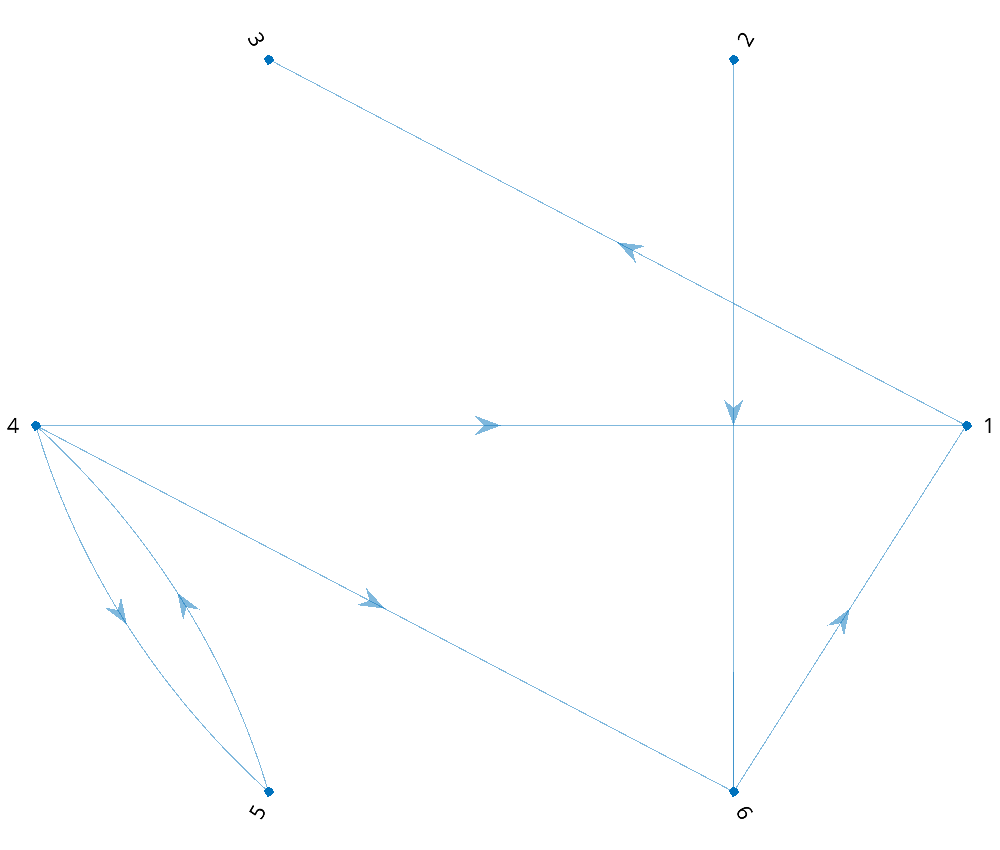
\includegraphics[scale=0.9]{../figures/A1_graph.png}
\end{center}

Vediamo quindi che le adiacenze fra nodi (pensando alla matrice, le dipendenze riga-colonna) sono:
\begin{table}[h!]
	\center \rowcolors{2}{white}{black!10}
	\begin{tabular} { c || c | c }
		\bfseries Nodo & \bfseries Raggiungibile & \bfseries Non raggiungibile \\
		\hline 
		1 & 1 3 & 2 4 5 6 \\
		2 & 1 2 3 6 & 4 5 \\
		3 & 3 & 1 2 4 5 6 \\
		4 & 1 3 4 5 6 & 2 \\
		5 & 1 3 4 5 6 & 2 \\
		6 & 1 3 6 & 2 4 5
	\end{tabular}
\end{table}

Notiamo che il nodo 6 ci fornisce la partizione migliore: $3 \times 3$ e $3 \times 3$.
Decidiamo quindi di prendere:
$$
\mathcal{P} = \{ 1, 3, 6 \}, \quad \mathcal{Q} = \{ 2, 4, 5 \}
$$
per cui la permutazione che manda $\mathcal{Q}$ in testa è:
$$
\Pi = \begin{pmatrix}
	0 & 1 & 0 & 0 & 0 & 0 \\
	0 & 0 & 0 & 1 & 0 & 0 \\
	0 & 0 & 0 & 0 & 1 & 0 \\
	1 & 0 & 0 & 0 & 0 & 0 \\
	0 & 0 & 1 & 0 & 0 & 0 \\
	0 & 0 & 0 & 0 & 0 & 1 \\
\end{pmatrix}
\begin{array}{c}
	2 \rightarrow 1 \\
	4 \rightarrow 2 \\
	5 \rightarrow 3 \\
	1 \rightarrow 4 \\
	3 \rightarrow 5 \\
	6 \rightarrow 6 \\
\end{array}
$$

Applicando $Pi A \Pi^T$ si ottiene quindi:
$$
\Pi A \Pi^T = \begin{pmatrix}
	A_{11} =
	\begin{pmatrix}
		2 &  0 &  0 \\
		0 &  2 & -1 \\
		0 & -1 &  2
	\end{pmatrix} &
	A_{12} = 
	\begin{pmatrix}
		0 &  0 &  3 \\
		3 &  0 & -2 \\
		0 &  0 &  0
	\end{pmatrix} \\
	0 &
	A_{21} = 
	\begin{pmatrix}
		1 &  1 &  0 \\
		0 & -1 &  0 \\
		1 &  0 &  1
	\end{pmatrix}
\end{pmatrix}
$$
che è una forma più agile per la risoluzione della matrice originale $A$.

Nella sottodirectory \lstinline|/code/matlab| si rende disponibile uno script \lstinline|block_decomp.m| per la decomposizione in matrici a blocchi come nell'esempio.
Un'esecuzione tipica dello script potrebbe avere l'aspetto:
\begin{lstlisting}[language=matlab, style=codestyle]	
p = block_decomp(A) % ottieni una permutazione
    Node      Reachable      Not reachable
    ____    _____________    _____________

     1      {[      1 3]}    {[  2 4 5 6]}
     2      {[  1 2 3 6]}    {[      4 5]}
     3      {[        3]}    {[1 2 4 5 6]}
     4      {[1 3 4 5 6]}    {[        2]}
     5      {[1 3 4 5 6]}    {[        2]}
     6      {[    1 3 6]}    {[    2 4 5]}
   
	 Choose an index: 6 % chiesto dallo script
>> A(p, p) % permuta A
\end{lstlisting}
da cui si ottiene la stessa matrice a blocchi riportata sopra.

\subsubsection{Riduzione iterata}
Ricordiamo di poter iterare ricorsivamente il processo di riduzione, cioè di poter trovare per ogni blocco $A_{ii}$ con $i \in \{ 1, 2 \}$ un $\Pi_i$ tale che:
$$
\Pi_i A_{ii} \Pi_i^T = \begin{pmatrix}
	A_{11}^{(i)} & A_{12}^{(i)} \\
	0 & A_{22}^{(i)} \\
\end{pmatrix}
$$
così che valga:
$$
\begin{pmatrix}
	\Pi_1 & 0 \\
	0 & \Pi_2
\end{pmatrix}
\begin{pmatrix}
	A_{11} & A_{12} \\
	0 & A_{22}
\end{pmatrix}
\begin{pmatrix}
	\Pi_1^T & 0 \\
	0 & \Pi_2^T
\end{pmatrix} =
\begin{pmatrix}
	\Pi_1 A_{11} \Pi_1^t & \Pi_1 A_{12} \Pi_2^T \\
	0 & \Pi_2 A_{22} \Pi_2^t \\
\end{pmatrix}
$$
$$
= \begin{pmatrix}
\begin{pmatrix}
	A_{11}^{(1)} & A_{12}^{(1)} \\
	0 & A_{22}^{(1)} \\
\end{pmatrix} & * \\
0 & 
\begin{pmatrix}
	A_{11}^{(2)} & A_{12}^{(2)} \\
	0 & A_{22}^{(2)} \\
\end{pmatrix}
\end{pmatrix}
$$
e via dicendo,
dove in $(*)$ comparrà qualcosa che al momento non ci interessa.

\subsubsection{Problemi agli autovalori per riduzione}
Notiamo che questo procedimento semplifica anche la risoluzione dei \textbf{problemi agli autovalori}: infatti iterando abbastanza, il problema si ridurrà a trovare i singoli autovalori di matrici sulla diagonale sempre più piccole, e quindi dal polinomio caratteristico di più facile risoluzione.

\subsection{Sistemi lineari}
Veniamo quindi alla trattazione dei sistemi lineari, che avevamo definito come forme $Ax = b$ con $A \in \mathbb{C}^{n \times n}, b \in \mathbb{C}^n$.

Studieremo 2 tipi di metodi risolutivi:
\begin{itemize}
	\item \textbf{Metodi diretti:} esatti ma dispendiosi, se eseguiti in aritmetica esatta (cioè senza arrotondamenti) poterebbero in un numero $n$ finito di passaggi alla soluzione esatta.
	Esempi di metodi diretti sono il \textbf{metodo di Cramer} (visto in 4.7.2) e l'\textbf{eliminazione di Gauss} (che vedremo fra poco);
	\item \textbf{Metodi iterativi:} meno accurati ma più efficienti computazionalmente, portano ad una successione $\{x_k\}_{k \in \mathbb{N}}$ di approssimazioni tali che $ \lim_{k \rightarrow +\infty} x_k = x$ soluzione esatta. Notiamo però che, in generale, è impossibile trovare il valore esatto di $x$ in un numero esatto di iterazioni. Per contropartita, risultano spesso molto più efficienti dei metodi diretti (esistono esempi di sistemi addirittura non risolvibili, nella pratica, con metodi diretti). 
\end{itemize}

\subsection{Metodi diretti per i sistemi lineari}
Iniziamo a trattare i metodi diretti per la risoluzione dei sistemi lineari.

\subsubsection{Sistemi triangolari}
Diamo la definizione parallela a quella di matrice triangolare:
\begin{definition}{Sistema triangolare}
	Si dice sistema triangolare un sistema della forma $Ux = c$ con $U$ matrice triangolare.
\end{definition}

Per un \textbf{sistema triangolare superiore}, si avrà la forma:
\[
\begin{cases}
    \begin{aligned}
			&& u_{11} x_1 + u_{12} x_2 + ... + u_{1,n-1} x_{n-1} + u_{1n} x_n = c_1 \\
			&&              u_{22} x_2 + ... + u_{2,n-1} x_{n-1} + u_{2n} x_n = c_2 \\
			&& \vdots \\
			&&                                 u_{n-1,n-1} x_{n-1} + u_{n-1,n} x_n = c_{n-1} \\
			&&                                                     u_{nn} x_n = c_n
		\end{aligned}
\end{cases}
\]

Il \textbf{metodo risolutivo} sarà allora la \textit{sostituzione all'indietro}, definita ricorsivamente come:
\[
	\begin{cases}
		x_n = \frac{c_n}{u_{nn}} \\\\ 
		x_i = \frac{ c_i - \sum_{j = i + 1}^n u_{ij} x_j }{u_{ii}}
	\end{cases}
\]
che equivale all'algoritmo, in MATLAB:
\lstinputlisting{../code/matlab/bck_subst.m}

Riguardo alla complessità, si potra dire che al passo $i$ si eseguono $n - i + n - i + 2 = 2(n - 1) + 2$ passaggi, cioè 2 per la divisione per $u_{jj}$ e la somma fra $c_i$ e il termine accumulato a destra, $n - i$ per i prodotti nella sommatoria e di nuovo $n - i$ per la sommatoria stessa.
Sarà allora che:
$$
\sum_{i = 1}^n \left( 2(n - i) + 2 \right) \sim O(n^2)
$$
cioè si ha complessità quadratica.

Osserviamo poi che per \textbf{sistemi triangolari inferiori} la situazione è uguale, cioè si risolve la prima equazione, si sostituisce il risultato nella seconda, e via dicendo:
\[
	\begin{cases}
		x_1 = \frac{c_1}{u_{11}} \\\\ 
		x_i = \frac{ c_i - \sum_{j = 1}^{i - 1} u_{ij} x_j }{u_{ii}}
	\end{cases}
\]
che equivale all'algoritmo, in MATLAB:
\lstinputlisting{../code/matlab/fwd_subst.m}

Il metodo ottenuto, speculare al quello di sostituzione all'indietro, viene detto \textit{sostituzione in avanti}, di costo identico ($O(n^2)$).

\subsubsection{Metodo di eliminazione di Gauss}
L'idea del metodo di eliminazione di Gauss è quella di partire da un sistema $Ax = b$, trasformarlo in un sistema equivalente $Ux = c$ (quindi triangolare superiore), ed applicare la sostituzione all'indietro.

Per arrivare alla forma $Ux = c$ si sostituiscono le equazioni del sistema con loro combinazioni lineari scelte in modo da annullare gli elementi inferiori alla diagonale.

L'idea è quella di eliminare, per ogni elemento $i$-esimo sulla diagonale a partire da quello in alto a destra, gli $n - i$ elementi che stanno al di sotto, cioè:

\begin{algorithm}
\caption{Eliminazione di Gauss}
\begin{algorithmic}
	\STATE \textbf{Input:} un sistema lineare qualsiasi $Ax = b$ % input
	\STATE \textbf{Output:} un sistema lineare triangolare superiore $Ux = c$ % output
	% body
	\FOR{$i = 1$ to $n$}
		\FOR{$j = i$ to $n$}
			\STATE Calcola il \textbf{moltiplicatore} $l_{ji} = \frac{a_{ji}^{(i - 1)}}{a_{ii}^{(i - 1)}}$
			\STATE Aggiungi alla riga $j$ la riga $i$ moltiplicata per $l_{ij}$
		\ENDFOR
	\ENDFOR
\end{algorithmic}
\end{algorithm}

\subsubsection{Implementazione MATLAB del metodo di eliminazione Gauss}
Una semplice implementazione in MATLAB del suddetto algoritmo può essere la seguente:
\begin{lstlisting}[language=matlab, style=codestyle]	
function [A, b] = gauss_decomp(A, b)
    n = height(A);

    for i = 1:n % i itera sulle diagonali
        den = A(i, i);

        for j = (i + 1):n % j itera sulle righe
            mul = A(j, i) / den; % moltiplicatore
            
            A(j, :) = A(j, :) - A(i, :) * mul;
            b(j) = b(j) - b(i) * mul;
        end
    end
end
\end{lstlisting}
da cui si potrà ottenere una riduzione di Gauss semplicemente come:
\begin{lstlisting}[language=matlab, style=codestyle]	
	>> [U, c] = gauss_decomp(A, b)
\end{lstlisting}

\par\smallskip

Dal punto di vista della complessità, la riduzione in forma triangolare costa $O(\frac{2}{3}n^3)$, e chiaramente domina sul termine $O(n^2)$ della risoluzione di $Ux = c$ con la sostituzione all'indietro.

Facciamo una nota sulla fattibiltà della riduzione di Gauss, definendo:
\begin{definition}{Moltiplicatori di Gauss}
	I termini $l_{ji} = \frac{a_{ji}^{(i - 1)}}{a_{ii}^{(i - 1)}}$ vengono detti moltiplicatori.
\end{definition}
Chiaramente, per poter eseguire l'eliminazione di Gauss serve che $a_{jj^{j - 1}} \neq 0$ $\forall j = 1, ..., n - 1$.
Inoltre, i casi $a_{jj}^{j - 1} \approx 0$ possono causare problemi di instabilità numerica.
Vedremo in seguito metodi per ovviare a questo problema.

\subsubsection{Fattorizzazione LU}
Il primo passo dell'algoritmo di Gauss si può vedere come equivalente a moltiplicare l'equazione $Ax = b$ a sinistra per una particolare matrice $H_1$ triangolare inferiore:
$$
H_1 = \begin{pmatrix}
	1 & ... & ... & 0 \\
	-l_{21} & 1 & ... & 0 \\
	... \\ 
	-l_{n1} & ... & ... & 1
\end{pmatrix}
$$
con la diagonale a $1$ e i moltiplicatori sulla prima colonna, così che $H_1 A$ risulti esattamente quello che volevamo per Gauss, cioè la combinazione lineare di ogni riga $j$ con l'prima riga moltiplicata per il moltiplicatore $l_{j1}$ (con $j > 2$).

Possiamo generalizzare questo processo a una serie di matrici $H_i$, per ogni elemento sulla diagonale, con la diagonale a $1$ e i moltiplicatori corrispondenti a $i$ sulla $i$-esima colonna:
$$
H_i = \begin{pmatrix}
	1 & ... & ... & 0 \\
	0 & 1 & ... & 0 \\
	... & -l_{ji} & ... & ... \\
	0 & -l_{ni} & ... & 1
\end{pmatrix}
$$
Così, ancora una volta, $A H_i$ risulterà quello che volevamo per Gauss, cioè la combinazione lineare di ogni riga $j$ con l'$i$-esima riga moltiplicata per il moltiplicatore $l_{ji}$.

Varrà allora he il metodo di Gauss sarà equivalente a considerare:
$$
H_{n - 1} H_{n - 2} \, ... \, H_1 A x = H_{n - 1} H_{n - 2} \, ... \, H_1 b
$$
e potremo quindi dire:
$$
H_{n - 1} H_{n - 2} \, ... \, H_1 A = U, \quad L = H_1^{-1} \, ... \, H_{n - 1}^1 
$$
da cui:
$$
A = LU
$$

Semplifichiamo i calcoli notando alcune proprietà delle matrici $H_j$:
\begin{enumerate}
	\item Hanno l'inversa facile, in quanto basta invertire i segni:
	$$
	H_i^{-1} = \begin{pmatrix}
		1 & ... & ... & 0 \\
		0 & 1 & ... & 0 \\
		... & l_{ji} & ... & ... \\
		0 & l_{ni} & ... & 1
	\end{pmatrix}
	$$

	\item Sono facili da moltiplicare, in quanto si può dire:
	$$
		H_{i_1} \cdot H_{i_2} = \begin{pmatrix}
		1 & ... & ... & 0 \\
		-l_{2i_1} & 1 & ... & 0 \\
		... & -l_{ji_2} & ... & ... \\
		-l_{ni_i} & -l_{ni_2} & ... & 1
	\end{pmatrix}
	$$
	e:	
	$$
	H_{i_1}^{-1} \cdot H_{i_2}^{-1} = \begin{pmatrix}
		1 & ... & ... & 0 \\
		l_{2i_1} & 1 & ... & 0 \\
		... & l_{ji_2} & ... & ... \\
		l_{ni_i} & l_{ni_2} & ... & 1
	\end{pmatrix}
	$$

	cioè semplicemente si somma sotto la diagonale.
\end{enumerate}

Questo significa che una volta svolta la prima parte dell'eliminazione di Gauss si è gia calcolata la fattorizzazione LU come la matrice dei moltiplicatori:
$$
H_{i_1}^{-1} \cdot H_{i_2}^{-1} = \begin{pmatrix}
	1 & ... & ... & 0 \\
	l_{21} & 1 & ... & 0 \\
	... & l_{3,2} & ...\\
	l_{n1} & l_{n2} & ... & 1
\end{pmatrix}
$$

\subsubsection{Implementazione MATLAB della riduzione LU}
Modifichiamo il codice MATLAB della scorsa sezione per calcolare, oltre all'eliminazione di Gauss (cioè la matrice $U$), la matrice dei moltiplicatori $L$:
\begin{lstlisting}[language=matlab, style=codestyle]	
function [A, b, L] = gauss_decomp(A, b)
    n = height(A);

    L = eye(n); % prepara L

    for i = 1:n % i itera sulle diagonali
        den = A(i, i);

        for j = (i + 1):n % j itera sulle righe
            mul = A(j, i) / den; % moltiplicatore
            L(j, i) = mul;
            
            A(j, :) = A(j, :) - A(i, :) * mul;
            b(j) = b(j) - b(i) * mul;
        end
    end
end
\end{lstlisting}

A questo punto per calcolare la fattorizzazione LU di una matrice basterà eseguire:
\begin{lstlisting}[language=matlab, style=codestyle]	
>> [U, ~, L] = gauss_decomp(A, b)
>> L * U % idealmente dara' A
\end{lstlisting}

\par\medskip

Si osserva quindi che se già si conoscono $L$ ed $U$ (magari di una matrice che dovremo usare spesso) risolvere $Ax = b$ costa $O(n^2)$, in quanto basta dire:
$$
Ax = b \, \Rightarrow \, LUx = b \implies x = U^{-1} L^{-1} b
$$
dove basta risolvere a cascata:
\[
	\begin{cases}
		Ly = b \\\
		Ux = y
	\end{cases}
\]
Questi sono due sistemi triangolari, uno \textbf{inferiore} (risolvibile per \textit{sostituzione in avanti}), l'altro \textbf{superiore} (risolvibile per \textit{sostituzione all'indietro}), da cui l'andamento complessivo $O(n^2)$.

In MATLAB, la soluzione si può quindi avere usando le funzioni definite finora:
\begin{lstlisting}[language=matlab, style=codestyle]	
>> [U, ~, L] = gauss_decomp(A, b)
>> y = fwd_subst(L, b)
>> x = bck_subst(U, y) % x e' la soluzione del sistema
\end{lstlisting}

Notiamo che questo vale se $L$ ed $U$ sono note (o come nell'esempio vengono calcolate), quindi tolto il prezzo dato dal doverle calcolare (come avevamo notato, conviene per matrici che magari dobbiamo usare spesso).

\subsubsection{Metodo di Gauss per variabili matriciali}
Se si vuole risolvere $AX = B$ con $X$ e $B$ matrici di vettori colonna di $s$ colonne:
$$
X = \begin{pmatrix}
	x_1 & ... & x_s
\end{pmatrix}, \quad
B = \begin{pmatrix}
	b_1 & ... & b_s
\end{pmatrix}
$$
cioè se si vogliono risolvere $s$ sistemi lineari con la stessa matrice $A$:
$$
Ax_1 = b_1, \quad ..., \quad Ax_s = b_s
$$
si può modificare l'algoritmo di Gauss, effettuando le mosse di Gauss sulla matrice aumentata $\begin{pmatrix}
	A \, | \, B
\end{pmatrix}$.
Alla fine troveremo una matrice $\begin{pmatrix}
	U \, | \, B^{(n - 1)}
\end{pmatrix}$, dove gli apici $(n - 1)$ rappresentano che è la $B$ che si ottiene all'$n-1$-esimo passaggio, che risolverà i sistemi triangolari superiori:
$$
Ux_1 = b_1^{(n - 1)}, \quad ..., \quad Ux_s = b_s^{(n - 1)}
$$

\par\smallskip

Vediamo un esempio numerico.
Partiamo dalle matrici $A$ e $B$:
$$
A = \begin{pmatrix}
	-2 & 1 & 1 \\ 
	-1 & 3 & 1 \\ 
	1 & 1 & 2
\end{pmatrix}, \quad B = \begin{pmatrix}
	-2 & 0 \\ 
	-3 & 0 \\ 
	2 & 1
\end{pmatrix}
$$
Avremo che le due colonne di $B$ rappresentano due vettori "termini noti" diversi, e che quindi la soluzione $X$ di $AX = B$ rappresenterà in verità due vettori soluzione:
$$
X = \begin{pmatrix}
	x_1^{(1)} & x_1^{(2)} \\
	x_2^{(1)} & x_2^{(2)} \\
	x_3^{(1)} & x_3^{(2)} \\
\end{pmatrix}
$$

Costruiamo quindi la matrice $AB$ ed applichiamo il metodo di riduzione di Gauss:
$$
AB = 
\left(\begin{array}{@{}c c c | c c@{}}
	-2 & 1 & 1 & -2 & 0 \\
	-1 & 3 & 1 & -3 & 0 \\
	1 & 1 & 2 & 2 & 1
\end{array}\right) \xrightarrow{\text{Gauss}}
\left(\begin{array}{@{}c c c | c c@{}}
	-2 & 1 & 1 & -2 & 0 \\
	0 & \frac{5}{2} & \frac{1}{2} & -2 & 0 \\ 
	0 & 0 & \frac{11}{5} & \frac{11}{5} & 1
\end{array}\right) = UB^{(n - 1)}
$$

Avremo quindi due sistemi dati dalla forma $UX = B^{(n - 1)}$:

\begin{minipage}{0.45\textwidth}

	\[
		x^{(1)} :
		\begin{cases}
			-2 x_1^{(1)} + x_2^{(1)} + x_3^{(1)} = -2 \\ 
			\frac{5}{2} x_2^{(1)} + \frac{1}{2} x_3^{(1)} = -2 \\ 
			\frac{11}{5} x_3^{(1)} = \frac{11}{5}
		\end{cases}
	\]

\end{minipage}%
\hfill % This adds horizontal space between the two minipages
\begin{minipage}{0.45\textwidth}

	\[
		x^{(2)} :
		\begin{cases}
			-2 x_1^{(2)} + x_2^{(2)} + x_3^{(2)} = 0 \\ 
			\frac{5}{2} x_2^{(2)} + \frac{1}{2} x_3^{(2)} = 0 \\ 
			\frac{11}{5} x_3^{(2)} = 1
		\end{cases}
	\]

\end{minipage}

da cui le soluzioni:
$$
x^{(1)} = \begin{pmatrix}
	1 \\ -1 \\ 1
\end{pmatrix} \quad 
x^{(2)} = \begin{pmatrix}
	\frac{2}{11} \\ -\frac{1}{11} \\ \frac{5}{11}
\end{pmatrix}
$$
e quindi la matrice incognita $X$:
$$
X = \begin{pmatrix}
	1 & \frac{2}{11} \\
	-1 & -\frac{1}{11} \\
	1 & \frac{5}{11} \\
\end{pmatrix}
$$


\subsubsection{Implementazione MATLAB del metodo di Gauss}
Implementiamo un risolutore per sistemi lineari, per comprendere a pieno questo risultato.
Vogliamo calcolare $X$ come la soluzione del sistema $AX = B$, e capiamo quindi che quello che cerchiamo sono i vettori colonna $x_1, ..., x_n$ tali per cui:
$$
A x_1 = B_1, \quad ..., \quad A x_n = b_n
$$
con $b_i$ l'$i$-esimo vettore colonna di $B$.
Sfruttiamo allora l'eliminazione di Gauss per ricavare due matrici, $U$ e $B^{(n - 1)}$, tali che $Ux = B^{(n - 1)}$, con il vantaggio che $U$ è triangolare superiore e quindi risolvibile per sostituzione all'indietro.
Possiamo fare questo in MATLAB come:
\begin{lstlisting}[language=matlab, style=codestyle]	
AI = [A, B]
UB1 = gauss_decomp(AB) % modificando gauss_decomp per un solo argomento 
U = UB1(1:n, 1:n)
B1 = UB1(1:n, (n + 1):(n + s)
\end{lstlisting}

A questo punto potremo trovare le colonne $x_i$ come:
\begin{lstlisting}[language=matlab, style=codestyle]	
>> x1 = bck_subst(U, B1(1:n, 1))
>> x2 = bck_subst(U, B1(1:n, 2))
...
\end{lstlisting}
e infine concatenare le colonne come:
\begin{lstlisting}[language=matlab, style=codestyle]	
>> X = [x1, ..., xn]
\end{lstlisting}
che realizzato in un unico script risulta:
\lstinputlisting{../code/matlab/gauss_solve.m}

\subsubsection{Metodo di Gauss per il calcolo dell'inversa}
Un caso particolare è il \textbf{calcolo dell'inversa} con l'algoritmo di \textbf{Gauss-Jordan}.
Infatti, scegliendo:
$$
AX = I
$$
con $n = s$, le colonne in $X$ diventeranno l'inversa di $A$ (basti vedere che $A A^{-1} = I$ per definizione).

\par\smallskip

Facciamo un esempio numerico.
Prendiamo la stessa matrice di prima:
$$
A = \begin{pmatrix}
	-2 & 1 & 1 \\ 
	-1 & 3 & 1 \\ 
	1 & 1 & 2
\end{pmatrix}
$$
e calcoliamone l'inversa come soluzione a $AX = I$.
Impostiamo quindi la matrice $AI$ e riduciamola:
$$
AI = 
\left(\begin{array}{@{}c c c | c c c@{}}
		-2 & 1 & 1 & 1 & 0 & 0 \\
		-1 & 3 & 1 & 0 & 1 & 0 \\
		1 & 1 & 2 & 0 & 0 & 1
\end{array}\right) \xrightarrow{\text{Gauss}}
\left(\begin{array}{@{}c c c | c c c @{}}
		-2 & 1 & 1 & 1 & 0 & 0 \\
		0 & \frac{5}{2} & \frac{1}{2} & -\frac{1}{2} & 1 & 0 \\ 
	0 & 0 & \frac{11}{5} & \frac{4}{5} & -\frac{3}{5} & 1
\end{array}\right) = UB^{(n - 1)}
$$
da cui i 3 sistemi lineari:

\begin{minipage}{0.35\textwidth}

	\[
	x^{(1)} :
		\begin{cases}
			-2 x_1^{(1)} + x_2^{(1)} + x_3^{(1)} = 1 \\ 
			\frac{5}{2} x_2^{(1)} + \frac{1}{2} x_3^{(1)} = -\frac{1}{2} \\ 
			\frac{11}{5} x_3^{(1)} = \frac{4}{5}
		\end{cases}
	\]

\end{minipage}%
\hfill
\begin{minipage}{0.35\textwidth}

	\[
	x^{(2)} :
		\begin{cases}
			-2 x_1^{(2)} + x_2^{(2)} + x_3^{(2)} = 0 \\ 
			\frac{5}{2} x_2^{(2)} + \frac{1}{2} x_3^{(2)} = 1 \\ 
			\frac{11}{5} x_3^{(2)} = -\frac{3}{5}
		\end{cases}
	\]

\end{minipage}
\[
x^{(3)} :
	\begin{cases}
		-2 x_1^{(3)} + x_2^{(3)} + x_3^{(3)} = 0 \\ 
		\frac{5}{2} x_2^{(3)} + \frac{1}{2} x_3^{(3)} = 0 \\ 
		\frac{11}{5} x_3^{(3)} = 1
	\end{cases}
\]
che hanno come soluzione:
$$
X = \begin{pmatrix}
	x^{(1)} & x^{(2)} & x^{(3)}
\end{pmatrix} = A^{-1} = \begin{pmatrix}
	-\frac{5}{11} & \frac{1}{11} & \frac{2}{11} \\ 
	-\frac{3}{11} & \frac{5}{11} & -\frac{1}{11} \\ 
	\frac{4}{11} & -\frac{3}{11} & \frac{5}{11}
\end{pmatrix}
$$

\subsubsection{Implementazione MATLAB del metodo di Gauss per il calcolo dell'inversa}
Facciamo un ultimo esempio MATLAB di questo procedimento.
Vogliamo calcolare $A^{-1}$ come la soluzione del sistema $AX = I$, e capiamo quindi che quello che cerchiamo sono i vettori colonna $i_1, ..., i_n$ tali per cui:
$$
A i_1 = I_1, \quad ..., \quad A i_n = I_n
$$
	con $I_i$ il vettore di zeri con un 1 all'$i$-esima riga. 
	Anche allora vogliamo sfruttare l'eliminazione di Gauss per ricavare due matrici, $U$ e $B^{(n - 1)}$, tali che $Ux = B^{(n - 1)}$, con il vantaggio che $U$ è triangolare superiore e quindi risolvibile per sostituzione all'indietro.

	Questo è esattamente quello che ci permette di fare la funzione \lstinline|gauss_solve()| definita prima, fissando il secondo argomento all'identità $I$ (in matlab \lstinline|eye(n)|):
	\lstinputlisting{../code/matlab/gauss_inv.m}

\end{document}


\documentclass[a4paper,11pt]{article}
\usepackage[a4paper, margin=8em]{geometry}

% usa i pacchetti per la scrittura in italiano
\usepackage[french,italian]{babel}
\usepackage[T1]{fontenc}
\usepackage[utf8]{inputenc}
\frenchspacing 

% usa i pacchetti per la formattazione matematica
\usepackage{amsmath, amssymb, amsthm, amsfonts}

% usa altri pacchetti
\usepackage{gensymb}
\usepackage{hyperref}
\usepackage{standalone}

% imposta il titolo
\title{Appunti Calcolo Numerico}
\author{Luca Seggiani}
\date{2025}

% disegni
\usepackage{pgfplots}
\pgfplotsset{width=10cm,compat=1.9}

% imposta lo stile
% usa helvetica
\usepackage[scaled]{helvet}
% usa palatino
\usepackage{palatino}
% usa un font monospazio guardabile
\usepackage{lmodern}

% tikz in sans
\tikzset{every picture/.style={/utils/exec={\sffamily}}}

\renewcommand{\rmdefault}{ppl}
\renewcommand{\sfdefault}{phv}
\renewcommand{\ttdefault}{lmtt}

% circuiti
\usepackage{circuitikz}
\usetikzlibrary{babel}

% disponi il titolo
\makeatletter
\renewcommand{\maketitle} {
	\begin{center} 
		\begin{minipage}[t]{.8\textwidth}
			\textsf{\huge\bfseries \@title} 
		\end{minipage}%
		\begin{minipage}[t]{.2\textwidth}
			\raggedleft \vspace{-1.65em}
			\textsf{\small \@author} \vfill
			\textsf{\small \@date}
		\end{minipage}
		\par
	\end{center}

	\thispagestyle{empty}
	\pagestyle{fancy}
}
\makeatother

% disponi teoremi
\usepackage{tcolorbox}
\newtcolorbox[auto counter, number within=section]{theorem}[2][]{%
	colback=blue!10, 
	colframe=blue!40!black, 
	sharp corners=northwest,
	fonttitle=\sffamily\bfseries, 
	title=Teorema~\thetcbcounter: #2, 
	#1
}

% disponi definizioni
\newtcolorbox[auto counter, number within=section]{definition}[2][]{%
	colback=red!10,
	colframe=red!40!black,
	sharp corners=northwest,
	fonttitle=\sffamily\bfseries,
	title=Definizione~\thetcbcounter: #2,
	#1
}

% disponi problemi
\newtcolorbox[auto counter, number within=section]{problem}[2][]{%
	colback=green!10,
	colframe=green!40!black,
	sharp corners=northwest,
	fonttitle=\sffamily\bfseries,
	title=Problema~\thetcbcounter: #2,
	#1
}

% disponi codice
\usepackage{listings}
\usepackage[table]{xcolor}

\definecolor{codegreen}{rgb}{0,0.6,0}
\definecolor{codegray}{rgb}{0.5,0.5,0.5}
\definecolor{codepurple}{rgb}{0.58,0,0.82}
\definecolor{backcolour}{rgb}{0.95,0.95,0.92}

\lstdefinestyle{codestyle}{
		backgroundcolor=\color{black!5}, 
		commentstyle=\color{codegreen},
		keywordstyle=\bfseries\color{magenta},
		numberstyle=\sffamily\tiny\color{black!60},
		stringstyle=\color{green!50!black},
		basicstyle=\ttfamily\footnotesize,
		breakatwhitespace=false,         
		breaklines=true,                 
		captionpos=b,                    
		keepspaces=true,                 
		numbers=left,                    
		numbersep=5pt,                  
		showspaces=false,                
		showstringspaces=false,
		showtabs=false,                  
		tabsize=2
}

\lstdefinestyle{shellstyle}{
		backgroundcolor=\color{black!5}, 
		basicstyle=\ttfamily\footnotesize\color{black}, 
		commentstyle=\color{black}, 
		keywordstyle=\color{black},
		numberstyle=\color{black!5},
		stringstyle=\color{black}, 
		showspaces=false,
		showstringspaces=false, 
		showtabs=false, 
		tabsize=2, 
		numbers=none, 
		breaklines=true
}

\lstdefinelanguage{javascript}{
	keywords={typeof, new, true, false, catch, function, return, null, catch, switch, var, if, in, while, do, else, case, break},
	keywordstyle=\color{blue}\bfseries,
	ndkeywords={class, export, boolean, throw, implements, import, this},
	ndkeywordstyle=\color{darkgray}\bfseries,
	identifierstyle=\color{black},
	sensitive=false,
	comment=[l]{//},
	morecomment=[s]{/*}{*/},
	commentstyle=\color{purple}\ttfamily,
	stringstyle=\color{red}\ttfamily,
	morestring=[b]',
	morestring=[b]"
}

% disponi sezioni
\usepackage{titlesec}

\titleformat{\section}
	{\sffamily\Large\bfseries} 
	{\thesection}{1em}{} 
\titleformat{\subsection}
	{\sffamily\large\bfseries}   
	{\thesubsection}{1em}{} 
\titleformat{\subsubsection}
	{\sffamily\normalsize\bfseries} 
	{\thesubsubsection}{1em}{}

% disponi alberi
\usepackage{forest}

\forestset{
	rectstyle/.style={
		for tree={rectangle,draw,font=\large\sffamily}
	},
	roundstyle/.style={
		for tree={circle,draw,font=\large}
	}
}

% disponi algoritmi
\usepackage{algorithm}
\usepackage{algorithmic}
\makeatletter
\renewcommand{\ALG@name}{Algoritmo}
\makeatother

% disponi numeri di pagina
\usepackage{fancyhdr}
\fancyhf{} 
\fancyfoot[L]{\sffamily{\thepage}}

\makeatletter
\fancyhead[L]{\raisebox{1ex}[0pt][0pt]{\sffamily{\@title \ \@date}}} 
\fancyhead[R]{\raisebox{1ex}[0pt][0pt]{\sffamily{\@author}}}
\makeatother

\begin{document}

% sezione (data)
\section{Lezione del 24-03-25}

% stili pagina
\thispagestyle{empty}
\pagestyle{fancy}

% testo
\subsection{Pivoting}
L'algoritmo di eliminazione di Gauss che abbiamo definito alla scorsa lezione ha un punto di fallimento nel caso uno degli elementi $a_{ii}^{(i - 1)}$ sia $= 0$, o comunque $\approx 0$, in quanto vorremmo a quel punto calcolare un moltiplicatore $l_{ji} = \frac{a_{ji}}{a_{ii}} \rightarrow$ non ben definito.

In tal caso si può modificare l'algoritmo sfruttando una matrice di permutazione che porti un elemento diverso da zero nella stessa posizione di $a_{ii}$.
Vorremo quindi cercare un indice $h$ tal per cui $a_{hi}^{(i - 1)}$ sia di modulo massimo nella sua colonna al di sotto di $i$, cioè:
$$
a_{hi}^{(i - 1)} \geq \max_{j = i, ..., n} | a_{ji}^{(i - 1)} |
$$
e scambiare la riga $i$ con la riga $h$.
Infatti, se $\det(A) \neq 0$, allora necessariamente esiste un $a_{ji}^{(i - 1)} \neq 0$ (altrimenti si ha uno 0 obbligato sulla diagonale, che con la matrice triangolare a blocchi dà $\det(A^{(i - 1)}) = 0$). \qed

Un altra conseguenza di questo approccio è che tutti i moltiplicatori $l_{ji}$ diventeranno $\leq 1$.
L'algoritmo di Gauss con questa modifica si chiama \textbf{eliminazione di Gauss con pivoting parziale} (\textit{parziale} perché ne esistono versioni più sofisticate, che non vedremo).

Osserviamo che ogni scambio di righe equivale a moltiplicare a sinistra per una matrice di permutazione $\Pi_i$.
Quindi il metodo di Gauss con pivoting può essere rappresentato come:
\begin{algorithm}
\caption{Eliminazione di Gauss con pivoting parziale}
\begin{algorithmic}
	\STATE \textbf{Input:} un sistema lineare qualsiasi $Ax = b$ % input
	\STATE \textbf{Output:} un sistema lineare triangolare superiore $Ux = c$ % output
	% body
	\FOR{$i = 1$ to $n$}
		\STATE Trova la matrice $\Pi_i$ che porta l'elemento di modulo massimo in testa
		\STATE $A \leftarrow \Pi_i A$
		\FOR{$j = i$ to $n$}
			\STATE Calcola il \textbf{moltiplicatore} $l_{ji} = \frac{a_{ji}^{(i - 1)}}{a_{ii}^{(i - 1)}}$
			\STATE Aggiungi alla riga $j$ la riga $i$ moltiplicata per $l_{ij}$
		\ENDFOR
	\ENDFOR
\end{algorithmic}
\end{algorithm}

\par\smallskip

Vediamo un esempio pratico dell'algoritmo prima di procedere all'implementazione MATLAB.
Prendiamo la matrice $A$ e il vettore $b$:
$$
A = \begin{pmatrix}
	1 & 2 & 3 \\ 
	4 & 5 & 6 \\ 
	7 & 8 & 0
\end{pmatrix}, \quad
b = \begin{pmatrix}
	1 \\ 2 \\ 3
\end{pmatrix}
$$
Nel ridurre la matrice aumentata $Ab$:
$$
\left(\begin{array}{@{}c c c | c@{}}
	1 & 2 & 3 & 1 \\ 
	4 & 5 & 6 & 2 \\ 
	7 & 8 & 0 & 3
\end{array}\right)
$$
ci accorgiamo che alla prima colonna l'entrata di modulo massimo è 7, di indice 3. Si permutano quindi la prima e la terza riga:
$$
\xrightarrow{\Pi_1}
\left(\begin{array}{@{}c c c | c@{}}
	7 & 8 & 0 & 3 \\
	4 & 5 & 6 & 2 \\ 
	1 & 2 & 3 & 1
\end{array}\right)
\xrightarrow{H_1 \Pi_1}
\left(\begin{array}{@{}c c c | c@{}}
		7 & 8 & 0 & 3 \\ 
		0 & \frac{3}{7} & 6 & \frac{2}{7} \\ 
		0 & \frac{6}{7} & 3 & \frac{4}{7}
\end{array}\right)
$$
nuovamente, l'entrata di modulo massimo è all'indice 3. Si permutano quindi la seconda e la terza riga:
$$
\xrightarrow{\Pi_2 H_1 \Pi_1}
\left(\begin{array}{@{}c c c | c@{}}
		7 & 8 & 0 & 3 \\ 
		0 & \frac{6}{7} & 3 & \frac{4}{7} \\
		0 & \frac{3}{7} & 6 & \frac{2}{7} 
\end{array}\right)
\xrightarrow{H_2 \Pi_2 H_1 \Pi_1}
\left(\begin{array}{@{}c c c | c@{}}
		7 & 8 & 0 & 3 \\ 
		0 & \frac{6}{7} & 3 & \frac{4}{7} \\
		0 & 0 & \frac{9}{2} & 0
\end{array}\right)
$$

\subsubsection{Implementazione MATLAB del metodo di eliminazione di Gauss con pivoting}
Modifichiamo quindi la funzione \lstinline|gauss_decomp()| per introdurre il meccanismo di pivoting appena visto:
\begin{lstlisting}[language=matlab, style=codestyle]	
function [A, b] = gauss_decomp(A, b)
    n = height(A);

    if nargin < 2
        b = zeros(n, 1);
    end

    for i = 1:n % i itera sulle diagonali
        % qui fai il pivot
        max_abs = max(abs(A(i:n, i)));
        h = find(abs(A(i:n, i)) == max_abs, 1);
        h = h + i - 1; % max abs si conta da i in poi

        A([i, h], :) = A([h, i], :); % permuta A
        b([i, h]) = b([h, i]); % permuta b
        
        den = A(i, i);

        for j = (i + 1):n % j itera sulle righe
            mul = A(j, i) / den; % moltiplicatore
            L(j, i) = mul;
            
            A(j, :) = A(j, :) - A(i, :) * mul;
            b(j) = b(j) - b(i) * mul;
        end
    end
end
\end{lstlisting}

\subsubsection{Fattorizzazione LU con pivoting}
Vediamo come ricavare una fattorizzazione LU dal metodo di Gauss modificato con il pivoting.
Si ha quindi che la matrice $U$ si evolve come:
$$
A \rightarrow \Pi_1 A \rightarrow H_1 \Pi_1 A \rightarrow ... \rightarrow H_{n - 1} \Pi_{n - 1} ... H_1 \Pi_1 A = U 
$$
mentre per la $L$ dovremo notare che:
$$
LU = \Pi A
$$
dove la matrice $\Pi$ rappresenta tutte le permutazioni fatte sulle righe di $A$.

Si ha quindi che:
\begin{itemize}
	\item $U$ è la matrice triangolare superiore trovata alla fine del metodo di Gauss con pivoting;
	\item $L$ è la matrice dei moltiplicatori, a cui però si devono applicare gli scambi delle righe, come segue: se al passo $i$ applico la matrice $\Pi_i$, devo applicare lo stesso cambio nelle prime $i - 1$ colonne di $L$, sotto la diagonale.
\end{itemize}

\par\smallskip 

Vediamo un esempio numerico spieghi il processo di formazione della matrice $L$ e della matrice di permutazione $\Pi$.
Presa la stessa matrice dell'esempio precedente:
$$
A = \begin{pmatrix}
	1 & 2 & 3 \\ 
	4 & 5 & 6 \\ 
	7 & 8 & 0
\end{pmatrix}
$$
abbiamo che le permutazioni sono, in sequenza:
$$
\Pi_1 : 
\begin{pmatrix}
	1 \\ 2 \\ 3
\end{pmatrix}
\rightarrow
\begin{pmatrix}
	3 \\ 2 \\ 1
\end{pmatrix}, \quad 
\Pi_2 :
\begin{pmatrix}
	3 \\ 2 \\ 1
\end{pmatrix}
\rightarrow
\begin{pmatrix}
	3 \\ 1 \\ 2
\end{pmatrix}
$$
o, in forma matriciale:
$$
\Pi_1 = \begin{pmatrix}
	0 & 0 & 1 \\ 
	0 & 1 & 0 \\ 
	1 & 0 & 0
\end{pmatrix}, \quad
\Pi_2 = \begin{pmatrix}
	1 & 0 & 0 \\ 
	0 & 0 & 1 \\ 
	0 & 1 & 0
\end{pmatrix}
$$

Calcoliamo quindi $L$.
$\Pi_1$ è irrilevante al calcolo di $L$, quindi la ignoriamo.
Vediamo che i primi due moltiplicatori sono $l_{21} = \frac{4}{7}$ e $l_{31} = \frac{1}{7}$, da cui si imposta $L^{(1)}$:
$$
L^{(1)} = \begin{pmatrix}
	1 & 0 & 0 \\ 
	\frac{4}{7} & 1 & 0 \\ 
	\frac{1}{7} & 0 & 1
\end{pmatrix}
$$

Notiamo quindi che dalla $\Pi_2$ dobbiamo scambiare gli elementi sotto la diagonale della prima colonna, quindi:
$$
L^{(1)} = \begin{pmatrix}
	1 & 0 & 0 \\ 
	\frac{1}{7} & 1 & 0 \\ 
	\frac{4}{7} & 0 & 1
\end{pmatrix}
$$

Infine, l'ultimo moltiplicatore $l_{32} = \frac{1}{2}$ non ha ambiguità:
$$
L^{(2)} = L = \begin{pmatrix}
	1 & 0 & 0 \\ 
	\frac{1}{7} & 1 & 0 \\ 
	\frac{4}{7} & \frac{1}{2} & 1
\end{pmatrix}
$$

Il calcolo di $\Pi$ deriva invece direttamente studiando la permutazione complessiva data dalle $\Pi_1, ..., \Pi_{n - 1}$, in questo caso:
$$
\Pi : \begin{pmatrix}
	1 \\ 2 \\ 3
\end{pmatrix}
\xrightarrow{\Pi_1}
\begin{pmatrix}
	3 \\ 2 \\ 1
\end{pmatrix}
\xrightarrow{\Pi_2}
\begin{pmatrix}
	3 \\ 1 \\ 2
\end{pmatrix}
$$
da cui:
$$
\Pi = \begin{pmatrix}
	0 & 0 & 1 \\ 
	1 & 0 & 0 \\ 
	0 & 1 & 0
\end{pmatrix}
$$

Con brevi calcoli si verifica che:
$$
LU = \Pi A
$$

\par\medskip 

\subsubsection{Implementazione MATLAB completa del metodo di eliminazione di Gauss con pivoting}
Vediamo quindi l'implementazione completa, che calcola anche la matrice $L$ e la matrice $\Pi$.
Notiamo inoltre l'argomento condizionale $b$, che viene ignorato se non fornito (abbiamo constatato che spesso è così).

\lstset{style=codestyle, language=matlab}
\lstinputlisting{../matlab/gauss_decomp.m}

\subsubsection{Determinante con pivoting}
Possiamo sfruttare la matrice $\Pi$ per il calcolo del determinante.
Si ha infatti dal teorema di Binet-Cauchy (4.1) che:
$$
\det(\Pi) \det(A) = \det(\Pi A) = \det(L U) = \det(L) \det(U)
$$
e quindi:
$$
\det(A) = \det(\Pi)^{-1} \det(L) \det(U)
$$
dove $\det(L) = 1$ (triangolare inferiore con diagonale di 1).
Si nota poi che $\det(\Pi)^{-1}$ è $(-1)^s$ è il numero di pivot che effettuiamo.
A questo punto $\det(U)$ è semplicemente il prodotto degli elementi sulla diagonale (triangolare superiore), cioè:
$$
\prod_{i = 1}^n a_{ii}^{(i - 1)} = \prod_{i = 1}^n u_{ii}
$$
e quindi:
$$
\det(A) = (-1)^s \prod_{i = 1}^n a_{ii}^{(i - 1)} = (-1)^s \prod_{i = 1}^n u_{ii}
$$
Si può quindi usare il metodo di Gauss, ancora una volta, per il calcolo del determinante di una matrice, con costo pari al costo dell'eliminazione di Gauss ($O(\frac{2}{3}n^3)$), molto meglio dello sviluppo di Laplace! ($O(n!)$).

\subsubsection{Implementazione MATLAB del metodo di Gauss per il determinante}
In MATLAB si può calcolare il prodotto delle diagonali come \lstinline|prod(diag(A))| e il segno di una permutazione come \lstinline|det(P)| (anche se sicuramente esistono approcci più efficienti).
Si può quindi realizzare uno script simile al seguente per il calcolo del determinante sfuttando \lstinline|gauss_decomp()| con permutazioni:
\lstinputlisting{../matlab/gauss_det.m}

\subsection{Condizionamento di un sistema lineare}
Date $A \in \mathbb{C}^{n \times n}$ e $b \in \mathbb{C}^n$, supponiamo di voler trovare $Ax = b$ ma a causa di errori nei dati o errori di arrotondamento troviamo (con un qualunque metodo) un vettore perturbato $x + \delta x \in \mathbb{C}^n$ che risolve un sistema lineare di per sé perturbato:
$$
(A + \delta A) (x + \delta x) = (b + \delta b)
$$
con $\delta A$ e $\delta B$ perturbazioni "piccole" della matrice $A$ e del vettore $b$, quindi $A + \delta A \in \mathbb{C}^{n \times n}$ e $b + \delta b \in \mathbb{C}^n$

La domanda è, se $\delta A$ e $\delta b$ sono piccole, posso concludere che anche $\delta x$ è relativamente piccolo?
Si scopre che la risposta a questa domanda è generalmente no.
Prendiamo ad esempio il sistema $2 \times 2$:
$$
\begin{pmatrix}
	1 & -1 \\
	1 & 1.000001
\end{pmatrix}
\begin{pmatrix}
	x_1 \\ x_2
\end{pmatrix}
=
\begin{pmatrix}
	1 \\ 1
\end{pmatrix}
$$
da cui $x$ esatto è $\begin{pmatrix}
	1 & 0
\end{pmatrix}$.
Perturbando $b$ a $\begin{pmatrix}
	0.999999 & 1
\end{pmatrix}$, si ha $x$ perturbato a $\begin{pmatrix}
	-10^{-6} & -1
\end{pmatrix}$, che è chiaramente un cambiamento drastico.
Viene da sé che agendo sulla matrice $A$ potremo ottenere effetti anche più drammatici.

\subsubsection{Condizionamento in $\mathbf{ \delta b}$}
Riprendiamo quindi la definizione di errore relativo:
$$
\epsilon = \frac{|\delta x|}{|x|}
$$
assumendo $\delta A = 0$ con $\det(A) \neq 0$, come nell'esempio precedente, e quindi perturbazioni solo del termine noto, si ha:
$$
A (x + \delta x) = (b + \delta b) \ \Leftrightarrow \ A\delta x = \delta b
$$
visto che $Ax = b$. Passando alle norme, si ha che:
$$
| \delta x | \leq |A^{-1}| \cdot |\delta b|
$$
e inoltre:
$$
|Ax| = |b| \implies |A| |x| \geq |b| \implies |x| \geq \frac{|b|}{|A|}
$$
quindi:
$$
\frac{|\delta x|}{|x|} \leq \frac{|A^{-1}| \cdot |\delta b| \cdot |A|}{|b|} = \frac{|\delta b|}{|b|} \cdot |A| \cdot |A^{-1}|
$$
dove ci interessa il valore $|A| \cdot |A^{-1}|$, l'unico che non dipende dall'errore assoluto $\delta b$.
\begin{definition}{Numero di condizionamento}
	Chiamiamo numero di condizionamento di una matrice $A$, data una certa norma $|\cdot|$, il valore:
	$$
		\mu(A) = |A| \cdot |A^{-1}|
	$$
\end{definition}

Abbiamo quindi che se $\mu(A) >> 1$, allora l'errore relativo può essere molto più grande dell'errore relativo dei dati e il problema si dice \textit{mal condizionato}.

\end{document}


\documentclass[a4paper,11pt]{article}
\usepackage[a4paper, margin=8em]{geometry}

% usa i pacchetti per la scrittura in italiano
\usepackage[french,italian]{babel}
\usepackage[T1]{fontenc}
\usepackage[utf8]{inputenc}
\frenchspacing 

% usa i pacchetti per la formattazione matematica
\usepackage{amsmath, amssymb, amsthm, amsfonts}

% usa altri pacchetti
\usepackage{gensymb}
\usepackage{hyperref}
\usepackage{standalone}

% imposta il titolo
\title{Appunti Calcolo Numerico}
\author{Luca Seggiani}
\date{2025}

% disegni
\usepackage{pgfplots}
\pgfplotsset{width=10cm,compat=1.9}

% imposta lo stile
% usa helvetica
\usepackage[scaled]{helvet}
% usa palatino
\usepackage{palatino}
% usa un font monospazio guardabile
\usepackage{lmodern}

% tikz in sans
\tikzset{every picture/.style={/utils/exec={\sffamily}}}

\renewcommand{\rmdefault}{ppl}
\renewcommand{\sfdefault}{phv}
\renewcommand{\ttdefault}{lmtt}

% circuiti
\usepackage{circuitikz}
\usetikzlibrary{babel}

% disponi il titolo
\makeatletter
\renewcommand{\maketitle} {
	\begin{center} 
		\begin{minipage}[t]{.8\textwidth}
			\textsf{\huge\bfseries \@title} 
		\end{minipage}%
		\begin{minipage}[t]{.2\textwidth}
			\raggedleft \vspace{-1.65em}
			\textsf{\small \@author} \vfill
			\textsf{\small \@date}
		\end{minipage}
		\par
	\end{center}

	\thispagestyle{empty}
	\pagestyle{fancy}
}
\makeatother

% disponi teoremi
\usepackage{tcolorbox}
\newtcolorbox[auto counter, number within=section]{theorem}[2][]{%
	colback=blue!10, 
	colframe=blue!40!black, 
	sharp corners=northwest,
	fonttitle=\sffamily\bfseries, 
	title=Teorema~\thetcbcounter: #2, 
	#1
}

% disponi definizioni
\newtcolorbox[auto counter, number within=section]{definition}[2][]{%
	colback=red!10,
	colframe=red!40!black,
	sharp corners=northwest,
	fonttitle=\sffamily\bfseries,
	title=Definizione~\thetcbcounter: #2,
	#1
}

% disponi problemi
\newtcolorbox[auto counter, number within=section]{problem}[2][]{%
	colback=green!10,
	colframe=green!40!black,
	sharp corners=northwest,
	fonttitle=\sffamily\bfseries,
	title=Problema~\thetcbcounter: #2,
	#1
}

% disponi codice
\usepackage{listings}
\usepackage[table]{xcolor}

\definecolor{codegreen}{rgb}{0,0.6,0}
\definecolor{codegray}{rgb}{0.5,0.5,0.5}
\definecolor{codepurple}{rgb}{0.58,0,0.82}
\definecolor{backcolour}{rgb}{0.95,0.95,0.92}

\lstdefinestyle{codestyle}{
		backgroundcolor=\color{black!5}, 
		commentstyle=\color{codegreen},
		keywordstyle=\bfseries\color{magenta},
		numberstyle=\sffamily\tiny\color{black!60},
		stringstyle=\color{green!50!black},
		basicstyle=\ttfamily\footnotesize,
		breakatwhitespace=false,         
		breaklines=true,                 
		captionpos=b,                    
		keepspaces=true,                 
		numbers=left,                    
		numbersep=5pt,                  
		showspaces=false,                
		showstringspaces=false,
		showtabs=false,                  
		tabsize=2
}

\lstdefinestyle{shellstyle}{
		backgroundcolor=\color{black!5}, 
		basicstyle=\ttfamily\footnotesize\color{black}, 
		commentstyle=\color{black}, 
		keywordstyle=\color{black},
		numberstyle=\color{black!5},
		stringstyle=\color{black}, 
		showspaces=false,
		showstringspaces=false, 
		showtabs=false, 
		tabsize=2, 
		numbers=none, 
		breaklines=true
}

\lstdefinelanguage{javascript}{
	keywords={typeof, new, true, false, catch, function, return, null, catch, switch, var, if, in, while, do, else, case, break},
	keywordstyle=\color{blue}\bfseries,
	ndkeywords={class, export, boolean, throw, implements, import, this},
	ndkeywordstyle=\color{darkgray}\bfseries,
	identifierstyle=\color{black},
	sensitive=false,
	comment=[l]{//},
	morecomment=[s]{/*}{*/},
	commentstyle=\color{purple}\ttfamily,
	stringstyle=\color{red}\ttfamily,
	morestring=[b]',
	morestring=[b]"
}

% disponi sezioni
\usepackage{titlesec}

\titleformat{\section}
	{\sffamily\Large\bfseries} 
	{\thesection}{1em}{} 
\titleformat{\subsection}
	{\sffamily\large\bfseries}   
	{\thesubsection}{1em}{} 
\titleformat{\subsubsection}
	{\sffamily\normalsize\bfseries} 
	{\thesubsubsection}{1em}{}

% disponi alberi
\usepackage{forest}

\forestset{
	rectstyle/.style={
		for tree={rectangle,draw,font=\large\sffamily}
	},
	roundstyle/.style={
		for tree={circle,draw,font=\large}
	}
}

% disponi algoritmi
\usepackage{algorithm}
\usepackage{algorithmic}
\makeatletter
\renewcommand{\ALG@name}{Algoritmo}
\makeatother

% disponi numeri di pagina
\usepackage{fancyhdr}
\fancyhf{} 
\fancyfoot[L]{\sffamily{\thepage}}

\makeatletter
\fancyhead[L]{\raisebox{1ex}[0pt][0pt]{\sffamily{\@title \ \@date}}} 
\fancyhead[R]{\raisebox{1ex}[0pt][0pt]{\sffamily{\@author}}}
\makeatother

\begin{document}

% sezione (data)
\section{Lezione del 28-03-25}

% stili pagina
\thispagestyle{empty}
\pagestyle{fancy}

% testo
Riprendiamo il discorso sull'errore inerente dei sistemi lineari.

Avevamo preso delle perturbazioni sulle matrici $A$ e $b$ (dovute a vari effetti reali, quali errori di arrotondamento, di misura, ecc...) nella forma:
$$
(A + \delta A) (x + \delta x) = (b + \delta b)
$$
e volevamo capire quanto può essere grande l'errore relativo $\frac{|\delta x|}{|x|}$, da:
$$
\frac{ \text{sol. perturbata} - \text{sol. reale} }{ \text{sol. reale} } = \frac{|x + \delta x - x|}{|x|} = \frac{|\delta x|}{|x|}
$$
Nel caso di $\delta A = 0$, abbiamo visto di poter maggiorare tale quantità come:
$$
\frac{|\delta x|}{|x|} \leq \mu(A) \cdot \frac{|\delta b|}{|b|}
$$
con $\mu(A) = |A| \cdot |A^{-1}|$ \textit{numero di condizionamento} (definizione 9.1).

Riguardo a $\mu(A)$, si ha che è $\geq 1$, cioè chiaramente non si può ridurre l'errore oltre la perfezione, e se $\mu(A) \approx 10^{k}$, $k$ è il numero di cifre significative che si \textit{perdono} nel risultato $x + \delta x$.

Possiamo quindi enunciare il seguente teorema:
\begin{theorem}{Condizionamento in $\mathbf{ \delta A }$}
	Se $|\delta A| \cdot |A^{-1}| < 1$ allora si ha:
	$$
	\frac{| \delta x|}{|x|} \leq \frac{\mu(A)}{1 - \mu(A) \cdot \frac{ |\delta A| }{|A|}} \cdot \left( \frac{|\delta A|}{|A|} + \frac{|\delta b|}{|b|} \right)
	$$
\end{theorem}
dove osserviamo che se $\delta A = 0$ si otiene la stessa diseguaglianza che abbiamo visto prima.

\subsubsection{Stima di $\mathbf{\mu}$}
In genere è abbastanza costoso calcolare il numero di condizionamento, in quanto bisogna calcolare un inversa e quindi la sua norma.
Quello che si può fare è cercarne una stima.

Ad esempio, se $A$ è hermitiana ($A = A^H$) e si considera la norma euclidea $|\cdot|_2$, si ha che:
$$
|A|_2 \cdot |A^{-1}|_2 = \rho(A) \cdot \rho(A^{-1}) = \frac{\lambda_\text{max}(A)}{\lambda_\text{min}(A)}
$$
cioè prendiamo il rapporto fra l'autovalore più grande e l'autovalore più piccolo di $A$, per cui si possono usare i metodi per gli autovalori (che vedremo verso la fine del corso).

\subsubsection{Stime a posteriori}
Supponiamo di aver calcolato $\tilde{x} \in \mathbb{C}^n$ con un qualunque metodo di approssimazione di $x$, prese $A$ e $b$ per buone.
Per valutare se $\tilde{x}$ è una \textit{buona} approssimazione basta guardare al \textbf{vettore residuo}, cioè:
$$
r = b - A \tilde{x}
$$

Potremmo chiederci se, con $|r|$ piccolo, si hanno anche $|x - \tilde{x}|$ piccoli.
Sottraiamo allora $Ax = b$ da $r$:
$$
A \left( x - \tilde{x} \right) = r \implies x - \tilde{x} = A^{-1} r
$$
e quindi vale la diseguaglianza:
$$
|x - \tilde{x} | \leq |A^{-1}| |r|
$$

Usando:
$$
|x| \geq \frac{|b|}{|A|}
$$
si otterrà allora che:
$$
\frac{|x - \tilde{x}|}{|x|} \leq \frac{ |A| |A^{-1}| |r| }{ |b| } = \mu(A) \cdot \frac{ |r| }{ |b| }
$$

Allora, in problemi ben condizionati, avremo che $\frac{ |x - \tilde{x}| }{|x|}$ errore relativo e $|r|$ sono comparabili, mentre in problemi con condizionamento $\mu(A) >> 1$ si potrebbe avere:
$$
\frac{ \frac{ |x - \tilde{x}| }{|x|} }{ |r| } \approx \mu(A)
$$

\subsection{Tecniche per l'approssimazione delle inverse}
Ogni volta che c'è bisogno di risolvere una forma del tipo:
$$
Ax = b \implies x = A^{-1} b
$$
il metodo naive sarebbe quello di calcolare $A^{-1}$ e moltiplicare per $b$.
Vediamo se si può fare di meglio.

Preso $n = 1$, la forma sarà quella di una semplice equazione lineare:
$$
ax = b. \implies x = \frac{b}{a}
$$
cioè basta fare una sola divisione, mentre l'approccio naive risulterebbe nel:
\begin{enumerate}
	\item Calcolare il reciproco $a^{-1}$;
	\item Moltiplicare il reciproco per $b \implies x = a^{-1} \cdot b$. 
\end{enumerate}
che chiaramente risulta in più passaggi, e quindi più approssimazioni intermedie e in definitiva maggiore errore.

\lstset{language=MATLAB, style=codestyle}

Nel caso matriciale il metodo di divisione equivale a fare una divisione matrice-vettore (che in MATLAB si effettua come \lstinline|A \ b|), di complessità $O( \frac{2}{3} n^3 )$.
Di contro, il metodo naive (che in MATLAB si effettua come \lstinline|inv(A) * b|) avrà complessità intorno ad $O( \frac{8}{3} n^3 )$, in quanto calcola la fattorizzazione LU e risolve 2n sistemi triangolari.

Inoltre, l'approccio naive è anche meno accurato, in quanto se il numero di condizionamento $\mu(A)$ è alto, l'errore di approssimazione nei passaggi intermedi potrebbe accumularsi molto di più che rispetto all'approccio della semplice divisione matrice-vettore (tanto che la stessa documentazione di MATLAB suggerisce di evitarlo).

\subsection{Metodi iterativi per i sistemi lineari}
Veniamo quindi a trattare i metodi iterativi per la risoluzione dei sistemi lineari.

L'idea è quella di approssimare la soluzione di un sistema lineare $Ax = b$ generando una successione di vettori $\{ x^{(k)} \}_{k \in \mathbb{N}}$ tali che:
$$
\lim_{k \rightarrow +\infty} x^{(k)} = x
$$
La motivazione è chiaramente quella di eludere l'alta complessità di $\sim O(n^3)$ che ha la risoluzione con metodi diretti.
Altra motivazione potrebbe essere quella di non conoscere direttamente $A$, ma solo l'applicazione:
$$
v \rightarrow A \cdot v
$$
(si pensi, anche se rappresenta un caso \textit{non} lineare, ai metodi di discesa a gradiente che ottimizzano funzioni non immediatamente calcolabili o anche solo esprimibili).

Abbiamo quindi che un buon metodo iterativo dovrà:
\begin{enumerate}
	\item Costare meno di $O(n^3)$ ad ogni passaggio (altrimenti sarebbe inutile rispetto ai metodi diretti), e quindi richiedere solo prodotti di matrici con vettori, o risoluzione di sistemi lineari favorevoli (triangolari, diagonali, ecc...);
	
	\item Data una certa \textbf{accuratezza} posta come obiettivo, impiegare un numero ragionevole di iterazioni per raggiungerla.
\end{enumerate}

\subsubsection{Metodi di punto fisso}
L'idea è quella di partire da $Ax - b = 0$ e di riscrivere come un'equazione equivalente in forma:
$$
x = Hx + c, \quad H \in \mathbb{C}^{n \times m}, \ c \in \mathbb{C}^n
$$

Facciamo alcuni esempi:
\begin{enumerate}
	\item Si sceglie una matrice $G \in \mathbb{C}^{n \times n}$ invertibile e si considera:
		$$
		x = x \cdot G(Ax - b) = (I - GA) x + Gb
		$$
		cioè:
		$$
		H = I - GA, \quad c = Gb
		$$

	\item Si scompone $A$ come:
		$$
		A = A_1 + A_2
		$$
		per cui:
		$$
		Ax = b \ \Leftrightarrow \ (A_1 + A_2) c = b \ \Leftrightarrow \ A_1 x = - A_2 x + b \ \Leftrightarrow \ x = -A_1^{-1} A_2 x + A_1^{-1} b
		$$
		cioè ancora:
		$$
		H = -A_1^{-1}A_2 , \quad c = A_1^{-1} b
		$$
\end{enumerate}

Una volta trovata un'equazione di punto fisso $x = H x + c$, quindi, si considera il seguente metodo iterativo:
\[
	\begin{cases}
		x^{(0)} \text{ dato} \\
		x^{(k + 1)} = H x^{(k)} + c, \quad k = 1, 2, 3, ...
	\end{cases}
\]
partendo da $x^{(0)}$ come dato a priori (sarà la soluzione che vorremo raffinare).

Vediamo che infatti:
\begin{definition}{Matrice di iterazione}
	La matrice $H$ di un equazione di punto fisso $x = H x + c$ viene detta matrice di iterazione.
\end{definition}

Per avere una verifica della validità dei metodi di punto fisso, enunciamo il seguente teorema:
\begin{theorem}{Validità dei metodi di punto fisso}
	Il metodo di punto fisso dato da:
\[
	\begin{cases}
		x^{(0)} \text{ dato} \\
		x^{(n + 1)} = H x^{(k)} + c, \quad k = 1, 2, 3, ...
	\end{cases}
\]
converge $\forall x^{(0)} \in \mathbb{C}^n$ se e solo se $\rho(H) < 1$.
\end{theorem}

Questo si dimostra prendendo l'equazione di punto fisso $x = H x + c$, soddisfatta da $x$ soluzione esatta, per cui:
$$
x^{(k + 1)} - x = H x^{(k)} + c - (H x + c) = H ( x^{(k)} - x )
$$

Possiamo chiamare $e^{(k)} = x^{(k)} - x$, cioè l'errore al passo $k$, e quindi l'errore al passo $k + 1$ sarà:
$$
e^{(k + 1)} = H e^{(k)} = H^k e^{(0)}
$$

Basterà allora prendere il limite:
$$
\lim_{k \rightarrow + \infty} e^{(k + 1)} = \lim_{k \rightarrow + \infty} H^k e^{(0)}
$$

Perchè questo tenda a $0$, basterà imporre $\rho(H) < 1$, in quanto in tal caso:
$$
\lim_{k \rightarrow + \infty} H^k e^{(0)} = 0
$$
qualsiasi sia l'errore iniziale $e^{(0)}$ (e quindi la scelta di soluzione iniziale $x^{(0)})$ \qed

In particolare, possiamo ricordare che se $|H| < 1 \implies \rho(H) < 1$, quindi può risultare verificare questa condizione, che è sì più stretta ma anche più facile da verificare.
Ricordiamo che non vale assolutamente il contrario, cioè $|H| > 1 \not \implies \rho(H) > 1$. # uff uff

Di contro, vale anche la condizione $|\det(H)| \geq 1 \implies \rho(H) > 1$, che come prima non si inverte in $|\det(H)| < 1 \not \implies \rho(H) < 1$.

\subsubsection{Velocità di convergenza}
Guardando alla dimostrazione del teorema 10.2, possiamo osservare che il raggio spettrale $\rho(H)$ ci dà un informazione anche riguardo alla \textbf{velocità di convergenza} del metodo di punto fisso.

Infatti, si avrà che vale:
$$
\frac{|e^{(k)}|}{|e^{(0)}|} \leq | H^k |
$$

Dall'algebra lineare, si ha che quando $k$ è abbastanza grande, $H^k \approx \rho(H)^k$, almeno per norme indotte, in quanto:
$$
\lim_{k \rightarrow +\infty} \sqrt[k]{|H^k|} = \rho(H)
$$

Questo ci dice che se si hanno 2 metodi di punto fisso con matrici di iterazione $H_1$ e $H_2$ tali che:
$$
\rho(H_1) < \rho(H_2) < 1
$$
allora il primo metodo converge più velocemente del secondo, è dall'ulteriore ipotesi $<1$, entrambi convergono.

Inoltre, si può stimare il numero di iterazioni $k$ necessarie a raggiungere un certo valore dell'errore:
$$
\frac{ | e^{(k)} | }{ | e^{(0)} | } = \frac{ | x^{(k)} - x | }{ | e^{(0)} | } \leq \delta 
$$
infatti, in tal caso basterà imporre:
$$
\rho(H)^k \leq \delta \implies k \geq \frac{ \log(\delta) }{\log( \rho(H) )}
$$

\subsubsection{Criteri di stop}
Molto spesso non è pratico decidere un errore e fare le $k$ iterazioni che dovrebbero portare a tale errore (in quanto non è scontato conoscere $\rho(H)$), ma bensì si preferisce definire un \textbf{criterio di stop} per la terminazione dell'algoritmo raggiunte determinate condizoni.

Queste condizioni possono essere:
\begin{enumerate}
	\item Si può restringere il residuo:
		$$
			\frac{ | r^{(k)} | }{ | b | } < \delta	
		$$
	\item Si può restringere direttamente la variazione di errore:
		$$
			| x^{k + 1} - x^{k} | < \delta	
		$$
\end{enumerate}

\subsection{Metodi di Jacobi e Gauss-Seidel}
Vediamo i metodi più famosi di questo tipo, detti metodi di \textbf{Jacobi} e \textbf{Gauss-Seidel}.

L'idea è di scomporre la matrice $A$ come:
$$
A = D - E - F
$$
con $D$ diagonale, $E$ l'opposta della triangolare inferiore a diagonale nulla e $F$ l'opposta della triangolare superiore a diagonale nulla. # scrivile
Varrà quindi:
$$
Ax = b \ \Leftrightarrow \ (D - E - F) x = b
$$

\subsubsection{Metodo di Jacobi}
Il metodo di Jacobi consiste nel riscrivere quanto trovato come:
$$
D x = (E + F) x + b \implies x = D^{-1} (E + F) x + D^{-1} b
$$
cioè trovare un equazione di punto fisso con:
$$
H = D^{-1} (E + F), \quad c = D^{-1} b
$$
e quindi applicare l'algoritmo:\[
	\begin{cases}
		x^{(0)} \text{ dato} \\
		x^{(k + 1)} = D^{-1} (E + F) x^{(k)} + D^{-1} b = D^{-1} ( (E + F) x^{(k)} + b )
	\end{cases}
\]

Osserviamo che ad ogni iterazione si calcola un prodotto matrice-vettore e si risolve un sistema diagonale ($O(n)$), in quanto la $D$ si inverte facilmente (è diagonale): # scrivile
$$
H_J = D^{-1} (E + F) = ...
$$

per cui:
$$
(H_j)_{ij} = 
\begin{cases}
	-\frac{ a_{ij} }{a_{ii}}, \quad i \neq j \\ 
	0 \quad i = j
\end{cases}
$$

Le matrici che descriveranno il passo di Jacobi saranno allora:
$$
x_i^{k + 1} = \frac{1}{a_{ii}} \left( b_i - \sum_{i \neq j}^n a_{ij} x_j^{(k)}  \right)
$$
osservando che per calcolare $x_i^{(k + 1)}$ servano \textit{tutte} le componenti di $x^{(k)}$, cioè in codice bisogna mantenere due vettori, in quanto non si può sovrascrivere $x^{(k)}$ prima di aver finito di calcolare $x^{(k + 1)}$.

# metti implementazione

\subsubsection{Metodo di Gauss-Seidel}
Il metodo di Gauss-Sidel consiste nel riscrivere quanto trovato come:
$$
(D - E) x = F x + b \implies x = (D - E)^{-1} F x + (D - E)^{-1} b
$$cioè trovare un equazione di punto fisso con:
$$
H = (D - E)^{-1} F, \quad c = (D - E)^{-1} b 
$$
e quindi applicare l'algoritmo:\[
	\begin{cases}
		x^{(0)} \text{ dato} \\
		x^{(k + 1)} = (D - E)^{-1} F x^{(k)} + (D - E)^{-1} b
	\end{cases}
\]

Avremo che la matrice di iterazione è:
$$
H_{GS} = (D - E)^{-1} F
$$
Osserviamo quindi che non si forma $H_{GS}$, ma ad ogni iterazione si calcola il prodotto matrice-vettore:
$$
x^{(k)} \rightarrow F x^{(k)}
$$
e si risolve:
$$
(D - E) y = F x^{(k)}
$$
Stesso discorso per $c$, che si trova risolvendo una sola volta il sistema lineare:
$$
(D - E) c = b
$$

Osserviamo poi che $H_{GS}$ ha come prima colonna il vettore di zeri in quanto $F$ ha anch'essa la prima colonna al vettore di zeri. # scrivile! (lui prende F = [ 0 | f2 ... f_n ])

# implementa

Vediamo quindi che, preso:
$$
x^{(k + 1)} = (D - E)^{-1} F x^{(k)} + (D - E)^{-1} b
$$
moltiplicando per $D^{-1}(D - E)$ si ha.
$$
x^{(k + 1)} = D^{-1} E x^{(k + 1)} + D^{-1} F x^{(k)} + D^{-1} b
$$

Esplicitare una dipendenza di $x^{(k + 1)}$ da se stessa potrebbe sembrare poco intuitivo,
ma è invece conveniente in quanto ogni elemento di $x^{(k + 1)}$ dipende dai soli elementi precedenti, cioè si ha:
$$
x_i^{(k + 1)} = \frac{1}{a_{ii}} \left( b_i - \sum_{j = 1}^{i - 1} a_{ij} x_j^{(k + 1)} - \sum_{j = i + 1}^n a_{ij} x_j^{(k)} \right), \quad i = 1, ..., n
$$

In questo modo si hanno due vantaggi:
\begin{enumerate}
	\item Non occorre risolvere sistemi triangolari;
	\item Per calcolare $x_i^{(k + 1)}$ non si ha bisogno di $x_h^{k}$ per $h < i$, e quindi si possono sovrascrivere le entrate di $x^{(k)}$, e mantenere un unico vettore.
\end{enumerate}

\par\medskip

Un'ultima osservazione è che sia Jacobi che Gauss-Seidel hanno come condizione che $a_{ii} \neq 0, \, \forall i$, in quanto altrimenti $D$ diagonale non sarebbe invertibile.
Se questa condizione non è soddisfatta, si possono fare delle trasformazioni "indolori" sul sistema per ritrovare la diagonale non nulla (applicare matrici di permutazione e applicare il metodo sul sistema permutato, per trovare poi una soluzione che al limite andrà \textit{de}-permutata).

Ad esempio, si può pensare di applicare Jacobi a:
$$
\Pi A x = \Pi b
$$
per trovare una qualche permutazione di $x$. # quale?

\end{document}


\documentclass[a4paper,11pt]{article}
\usepackage[a4paper, margin=8em]{geometry}

% usa i pacchetti per la scrittura in italiano
\usepackage[french,italian]{babel}
\usepackage[T1]{fontenc}
\usepackage[utf8]{inputenc}
\frenchspacing 

% usa i pacchetti per la formattazione matematica
\usepackage{amsmath, amssymb, amsthm, amsfonts}

% usa altri pacchetti
\usepackage{gensymb}
\usepackage{hyperref}
\usepackage{standalone}

% imposta il titolo
\title{Appunti Calcolo Numerico}
\author{Luca Seggiani}
\date{2025}

% disegni
\usepackage{pgfplots}
\pgfplotsset{width=10cm,compat=1.9}

% imposta lo stile
% usa helvetica
\usepackage[scaled]{helvet}
% usa palatino
\usepackage{palatino}
% usa un font monospazio guardabile
\usepackage{lmodern}

% tikz in sans
\tikzset{every picture/.style={/utils/exec={\sffamily}}}

\renewcommand{\rmdefault}{ppl}
\renewcommand{\sfdefault}{phv}
\renewcommand{\ttdefault}{lmtt}

% circuiti
\usepackage{circuitikz}
\usetikzlibrary{babel}

% disponi il titolo
\makeatletter
\renewcommand{\maketitle} {
	\begin{center} 
		\begin{minipage}[t]{.8\textwidth}
			\textsf{\huge\bfseries \@title} 
		\end{minipage}%
		\begin{minipage}[t]{.2\textwidth}
			\raggedleft \vspace{-1.65em}
			\textsf{\small \@author} \vfill
			\textsf{\small \@date}
		\end{minipage}
		\par
	\end{center}

	\thispagestyle{empty}
	\pagestyle{fancy}
}
\makeatother

% disponi teoremi
\usepackage{tcolorbox}
\newtcolorbox[auto counter, number within=section]{theorem}[2][]{%
	colback=blue!10, 
	colframe=blue!40!black, 
	sharp corners=northwest,
	fonttitle=\sffamily\bfseries, 
	title=Teorema~\thetcbcounter: #2, 
	#1
}

% disponi definizioni
\newtcolorbox[auto counter, number within=section]{definition}[2][]{%
	colback=red!10,
	colframe=red!40!black,
	sharp corners=northwest,
	fonttitle=\sffamily\bfseries,
	title=Definizione~\thetcbcounter: #2,
	#1
}

% disponi problemi
\newtcolorbox[auto counter, number within=section]{problem}[2][]{%
	colback=green!10,
	colframe=green!40!black,
	sharp corners=northwest,
	fonttitle=\sffamily\bfseries,
	title=Problema~\thetcbcounter: #2,
	#1
}

% disponi codice
\usepackage{listings}
\usepackage[table]{xcolor}

\definecolor{codegreen}{rgb}{0,0.6,0}
\definecolor{codegray}{rgb}{0.5,0.5,0.5}
\definecolor{codepurple}{rgb}{0.58,0,0.82}
\definecolor{backcolour}{rgb}{0.95,0.95,0.92}

\lstdefinestyle{codestyle}{
		backgroundcolor=\color{black!5}, 
		commentstyle=\color{codegreen},
		keywordstyle=\bfseries\color{magenta},
		numberstyle=\sffamily\tiny\color{black!60},
		stringstyle=\color{green!50!black},
		basicstyle=\ttfamily\footnotesize,
		breakatwhitespace=false,         
		breaklines=true,                 
		captionpos=b,                    
		keepspaces=true,                 
		numbers=left,                    
		numbersep=5pt,                  
		showspaces=false,                
		showstringspaces=false,
		showtabs=false,                  
		tabsize=2
}

\lstdefinestyle{shellstyle}{
		backgroundcolor=\color{black!5}, 
		basicstyle=\ttfamily\footnotesize\color{black}, 
		commentstyle=\color{black}, 
		keywordstyle=\color{black},
		numberstyle=\color{black!5},
		stringstyle=\color{black}, 
		showspaces=false,
		showstringspaces=false, 
		showtabs=false, 
		tabsize=2, 
		numbers=none, 
		breaklines=true
}

\lstdefinelanguage{javascript}{
	keywords={typeof, new, true, false, catch, function, return, null, catch, switch, var, if, in, while, do, else, case, break},
	keywordstyle=\color{blue}\bfseries,
	ndkeywords={class, export, boolean, throw, implements, import, this},
	ndkeywordstyle=\color{darkgray}\bfseries,
	identifierstyle=\color{black},
	sensitive=false,
	comment=[l]{//},
	morecomment=[s]{/*}{*/},
	commentstyle=\color{purple}\ttfamily,
	stringstyle=\color{red}\ttfamily,
	morestring=[b]',
	morestring=[b]"
}

% disponi sezioni
\usepackage{titlesec}

\titleformat{\section}
	{\sffamily\Large\bfseries} 
	{\thesection}{1em}{} 
\titleformat{\subsection}
	{\sffamily\large\bfseries}   
	{\thesubsection}{1em}{} 
\titleformat{\subsubsection}
	{\sffamily\normalsize\bfseries} 
	{\thesubsubsection}{1em}{}

% disponi alberi
\usepackage{forest}

\forestset{
	rectstyle/.style={
		for tree={rectangle,draw,font=\large\sffamily}
	},
	roundstyle/.style={
		for tree={circle,draw,font=\large}
	}
}

% disponi algoritmi
\usepackage{algorithm}
\usepackage{algorithmic}
\makeatletter
\renewcommand{\ALG@name}{Algoritmo}
\makeatother

% disponi numeri di pagina
\usepackage{fancyhdr}
\fancyhf{} 
\fancyfoot[L]{\sffamily{\thepage}}

\makeatletter
\fancyhead[L]{\raisebox{1ex}[0pt][0pt]{\sffamily{\@title \ \@date}}} 
\fancyhead[R]{\raisebox{1ex}[0pt][0pt]{\sffamily{\@author}}}
\makeatother

\begin{document}

% sezione (data)
\section{Lezione del 31-03-25}

% stili pagina
\thispagestyle{empty}
\pagestyle{fancy}

% testo
Riprendiamo la trattazione dei metodi iterativi per i sistemi lineari.

\subsubsection{Valutazione della convergenza}
Avevamo visto che affinché un metodo di punto fisso sia convergente è necessario che la sua matrice di iterazione $H$ in:
$$
x = H x + c
$$
sia convergente, cioè abbia norma spettrale $\rho(H) < 1$.

Vediamo un esempio di valutazione di tale matrice sia per il metodo di Jacobi e di Gauss-Siedel applicato ad una certa matrice $A$, svolgendo esplicitamente tutti i calcoli:
$$
A = \begin{pmatrix}
	1 & \frac{2}{3} & \frac{4}{9} \\
	\frac{2}{3} & 1 & \frac{2}{3} \\ 
	\frac{4}{9} & \frac{2}{3} & 1
\end{pmatrix}
$$

\begin{itemize}
	\item \textbf{Jacobi:} avremo la matrice di convergenza:
$$
x = \underbrace{D^{-1}(E + F)}_{H_J} x + D^{-1} b
$$
da cui:
$$
H_J = D^{-1}(E + F) = I \cdot \begin{pmatrix}
	0 & \frac{2}{3} & \frac{4}{9} \\
	\frac{2}{3} & 0 & \frac{2}{3} \\ 
	\frac{4}{9} & \frac{2}{3} & 0
\end{pmatrix}
$$
Calcoliamo quindi gli autovalori attraverso il polinomio caratteristico:
$$
p(\lambda) = \det \left( \lambda I - D^{-1} (E + F) \right) = \det \begin{pmatrix}
	\lambda & \frac{2}{3} & \frac{4}{9} \\
	\frac{2}{3} & \lambda & \frac{2}{3} \\ 
	\frac{4}{9} & \frac{2}{3} & \lambda
\end{pmatrix} = \lambda^3 + \frac{16}{81} \cdot 2 - \frac{16}{81} \lambda - 2 \cdot \frac{4}{9} \lambda
$$
per la regola di Sarrus, quindi:
$$
p(\lambda) = \lambda^3 - \frac{88}{81} \lambda + \frac{32}{81}
$$
Accorgiamoci che $\lambda_1 = \frac{4}{9}$ è radice del polinomio, e quindi dividiamo:
$$
\frac{ \lambda^3 - \frac{88}{81} \lambda + \frac{32}{81}}{\lambda - \frac{4}{9}} = \lambda^2 + \frac{4}{9} \lambda - \frac{8}{9} 
$$
per cui:
$$
p(\lambda) = \left( \lambda - \frac{4}{9} \right) \left( \lambda^2 + \frac{4}{9} \lambda - \frac{8}{9} \right)
$$
Risolviamo quindi la quadratica:
$$
\lambda_{2, 3} = \frac{-\frac{4}{9} \pm \sqrt{ \frac{16}{81} + \frac{32}{9} }}{2} = -\frac{2}{9} \left( 1 \mp \sqrt{19} \right)
$$
Delle 3 radici trovate si ha che $\lambda_3 = -\frac{2}{9} \left( 1 + \sqrt{19} \right) \approx - 1.19087$ è in modulo $\geq 0$, ergo la condizione di convergenza non è rispettata, e il metodo di Jacobi potrebbe non convergere.

	\item \textbf{Gauss-Seidel:} avremo la matrice di convergenza:
$$
x = \underbrace{(D - E)^{-1} F}_{H_{GS}} x + (D - E)^{-1} b
$$
da cui:
$$
H_{GS} = (D - E)^{-1} F  = \begin{pmatrix}
	1 & 0 & 0 \\ 
	\frac{2}{3} & 1 & 0 \\ 
	\frac{4}{9} & \frac{2}{3} & 1
\end{pmatrix}^{-1}
\begin{pmatrix}
	0 & -\frac{2}{3} & -\frac{4}{9} \\ 
	0 & 0 & -\frac{2}{3} \\ 
	0 & 0 & 0
\end{pmatrix}
$$
che sfruttando quanto avevamo detto sui prodotti per inverse:
$$
= \begin{pmatrix}
(D - E)^{-1} \begin{pmatrix}
	0 \\ 0 \\ 0
\end{pmatrix} & 
(D - E)^{-1} \begin{pmatrix}
	-\frac{2}{3} \\ 0 \\ 0
\end{pmatrix} & 
(D - E)^{-1} \begin{pmatrix}
	-\frac{4}{9} \\ -\frac{2}{3} \\ 0
\end{pmatrix} 
\end{pmatrix} 
$$
cioè dobbiamo risolvere 3 sistemi lineari (di cui uno banale) usando il metodo di sostituzione all'indietro.
Avremo quindi:
\begin{itemize}
	\item Il sistema:
$$
\begin{pmatrix}
	1 & 0 & 0 \\ 
	\frac{2}{3} & 1 & 0 \\ 
	\frac{4}{9} & \frac{2}{3} & 1
\end{pmatrix}
\begin{pmatrix}
	x \\ y \\ z
\end{pmatrix} =
\begin{pmatrix}
	-\frac{2}{3} \\ 0 \\ 0
\end{pmatrix}
$$
che dà:
$$
\begin{pmatrix}
	x \\ y \\ z
\end{pmatrix} = 
\begin{pmatrix}
	-\frac{2}{3} \\ \frac{4}{9} \\ 0
\end{pmatrix}
$$
	\item Il sistema:
$$
\begin{pmatrix}
	1 & 0 & 0 \\ 
	\frac{2}{3} & 1 & 0 \\ 
	\frac{4}{9} & \frac{2}{3} & 1
\end{pmatrix}
\begin{pmatrix}
	x \\ y \\ z
\end{pmatrix} =
\begin{pmatrix}
	-\frac{4}{9} \\ -\frac{2}{3} \\ 0
\end{pmatrix}
$$
che dà:
$$
\begin{pmatrix}
	x \\ y \\ z
\end{pmatrix} = 
\begin{pmatrix}
	-\frac{4}{9} \\ -\frac{10}{27} \\ \frac{4}{9}
\end{pmatrix}
$$
\end{itemize}
da cui:
$$
H_{GS} = \begin{pmatrix}
	0 & -\frac{2}{3} & -\frac{4}{9} \\ 
	0 & \frac{4}{9} & -\frac{10}{27} \\ 
	0 & 0 & \frac{4}{9}
\end{pmatrix}
$$
da cui $\lambda_1 = 0$ e $\lambda_2 = \frac{4}{9}$ con molteplicità $\mu_2 = 2$, quindi tutti gli autovalori a modulo $< 1$ e la condizione di convergenza è rispettata.
\end{itemize}

\subsubsection{Criteri di convergenza di matrici di iterazione}
Cerchiamo un modo più generale per fare ciò che abbiamo fatto nell'ultimo esempio.
Vediamo che vale il seguente teorema:
\begin{theorem}{Criteri di convergenza di matrici di iterazione}
	Se $A \in \mathbb{C}^{n \times n}$ rispetta una delle seguenti condizioni:
	\begin{enumerate}
		\item $A$ è ha predominanza diagonale forte;
		\item $A$ è irriducibile e a predominanza diagonale debole;
	\end{enumerate}
	allora sia il metodo di Jacobi che il metodo di Gauss-Seidel danno iterazioni convergenti applicati ad un sistema $Ax = b$. 
\end{theorem}

\begin{enumerate}
	\item 
La dimostrazione del teorema comincia dall'imporre che $a_{ii} \neq 0$, $\forall i = 1, ..., n$.
Avevamo visto che questa condizione può essere forzata scambiando $A$ con una qualche permutazione $\Pi A$.

Abbiamo allora che la condizione è ovvia nel caso di predominanza diagonale forte (1), mentre nel caso di matrice irriducibile a predominanza diagonale debole (2), se esistesse un $a_{ii} = 0$ per qualche $i$ allora applicando la predominanza diagonale debole si avrebbe $a_{ij} = 0$ ($0 \geq \sum_{i \neq j}^n a_{ij}$), che sarebbe assurdo (la matrice non può essere singolare).
Notiamo che in questo caso nemmeno una matrice di permutazione $\Pi$ potrebbe portarci a diagonale non negativa.

	\item 
Dimostriamo la convergenza per i due metodi:
\begin{itemize}
\item \textbf{Jacobi:} si ha che:
$$
H_J = D^{-1}(E + F) = \begin{pmatrix}
	0 & ... & -\frac{a_{ij}}{a_{ii}} \\ 
	... & 0 & ... \\ 
	-\frac{a_{ij}}{a_{ii}} & ... & 0
\end{pmatrix}
$$
e allora la norma a infinito di $H_J$ sarà:
$$
|H_J|_{\infty} = \max_{i = 1, ..., n} \sum_{i \neq j}^n \left|\frac{a_{ij}}{a_{ii}}\right|
$$
Se $A$ è a predominanza diagonale forte (1), allora $|a_{ii}| > \sum_{j \neq i}^n |a_{ij}|$, e quindi $|H_J|_\infty < 1$ e $\rho(H_j) < 1$.

Se $A$ è invece irriducibile a predominanza diagonale debole (2), sarà che nuovamente $|H_J|_\infty \leq 1$, quindi gli autovalori di $A$ sono $|\lambda| \leq 1$, ma non esiste $|\lambda| = 1$ in quanto starebbe sul bordo di un cerchio di Gershgorin, quindi di tutti, ma esiste almeno un cerchio $\mathcal{F}_i(A)$ con raggio $r < 1$. 

\item \textbf{Gauss-Seidel:} supponiamo che esista $\lambda^*$ autovalore di $H_{GS}$:
$$
H_{GS} = (D - E)^{-1} F
$$
tale che $|\lambda^*| \geq 1$.
Allora dovrà valere:
$$
0 = \det(\lambda^* I - H_{GS}) = \det\left (\lambda^* I - (D - E)^{-1} F \right) = \det \left( (D- E)^{-1} \left( \lambda(D - E) - F \right) \right)
$$
che per Binet-Cauchy dà:
$$
0 = \det \left( (D - E)^{-1} \right) \cdot \det \left(\lambda^* (D - E) - F \right)
$$
Il primo termine è chiaramente $\neq 0$, e quindi si considera:
$$
0 = \det \left( \lambda^* (D - E) - F \right) = \left(\lambda^*\right)^n \det \left(D - E - (\lambda^*)^{-1} F \right)
$$
cioè:
$$
0 = \det \left(D - E - (\lambda^*)^{-1} F \right)
$$
\end{itemize}
La matrice che troviamo è quella dove gli elementi sopra la diagonale hanno modulo $\leq$ ai corrispondenti nella matrice $A$.
Se $A$ è dominante diagonale forte o dominante diagonale debole, quindi, conserva tale proprietà, e conserva anche l'irriducibilità.
Quindi, necessariamente, è non singolare (altrimenti anche $A$ sarebbe singolare).
Allora, visto che per definizione $H_{GS}$ deve essere singolare (prima colonna nulla), l'ipotesi $|\lambda^*| \geq 1$ è assurda, cioè deve essere $|\lambda^*| < 1$.
\end{enumerate} \qed

\subsection{Sistemi rettangolari}
Vediamo quindi come risolvere sistemi \textbf{rettangolari}, cioè del tipo $Ax = b$ con $A \in \mathbb{C}^{m \times n}$ rettangolare.
In questo caso si avranno $m$ equazioni in $n$ incognite, quindi con $x \in \mathbb{C}^n$ e $b \in \mathbb{C}^m$.
Supponiamo poi che $A$ sia di rango massimo, ovvero $\mathrm{rank}(A) = \min(m, n)$.

Scopriamo che anche in questo scenario si può applicare l'eliminazione di Gauss, e nel caso $m < n$, si può immaginare di rendere il sistema quadrato aggiungendo $n - m$ equazioni fittizie della forma $0 = 0$, lasciando $n - m$ parametri liberi:

$$
\begin{pmatrix}
	1 & ... & ... & ... \\ 
	0 & 1 & ... & ... \\ 
	0 & ... & 1 & ... \\
	0 & ... & ... & 0 \\ 
	\vdots & & & \vdots \\ 
	0 & ... & ... & 0
\end{pmatrix}
\begin{pmatrix}
	x_1 \\ \vdots \\ x_m \\ x_{m + 1} \\ \vdots \\ x_n
\end{pmatrix}
=
\begin{pmatrix}
	b_1 \\ \vdots \\ b_m
\end{pmatrix}
$$

Diciamo che questo tipo di sistemi si dicono \textbf{sottodeterminati}.

Caso più interessante sarà quello dei sistemi \textbf{sovradeterminati}, cioè dove $n < m$ e si hanno più equazioni che incognite.
In questo caso l'applicazione dell'eliminazione di Gauss porta ad $n$ equazioni determinate, e $m  - n$ equazioni della forma $0 = \, ?$ dove $?$ sono i termini noti che si formano nelle ultime $m - n$ righe:

$$
\begin{pmatrix}
	1 & ... & ... \\ 
	0 & 1 & ... \\ 
	0 & ... & 1 \\ 
	0 & ... & 0 \\ 
	\vdots & & \vdots \\ 
	0 & ... & 0
\end{pmatrix}
\begin{pmatrix}
	x_1 \\ \vdots \\ x_n
\end{pmatrix} =
\begin{pmatrix}
	b_1 \\ \vdots \\ b_n \\ b_{n + 1} = \ ?_1 \\ \vdots \\ b_m = \ ?_{m - n + 1}
\end{pmatrix}
$$

Se esiste almeno un termine noto $? \neq 0$, allora il sistema è impossibile (ed è questo il caso tipico).
Questa affermazione è essenzialmente il teorema di Rouchè-Capelli, dove si impone:
$$
\mathrm{rank}(A | b) = \mathrm{rank}(A)
$$

Il problema che ci poniamo in questi casi è quello di minimizzare il residuo, cioè posto:
$$
x - Ab = r(x)
$$
cercare di risolvere il problema di ottimizzazione:
$$
r^* = \min_{x \in \mathbb{C}^n} |b - Ax|_2 = \min_{x \in \mathbb{C}^n} |r(x)|_2
$$

Questo tipo di problema viene detto \textbf{problema dei minimi quadrati}.
Osserviamo che il problema è equivalente a risolvere:
$$
\left(r^*\right)^2 = \min_{x \in \mathbb{C}^n} |b - Ax|_2^2 = \min_{x \in \mathbb{C}^n} |r(x)|_2^2
$$
Cioè ci possiamo liberare della radice della norma quadratica.

Potremo innanzitutto chiederci come trovare il punto $x^*$ che dà $r^*$, o in principio se questo problema ammette soluzione.
Facciamo allora un esempio del caso $x \in \mathbb{R}^n$
Considereremo la funzione:
$$
\psi(x) = |b - Ax|_2^2 = (b - Ax)^T (b - Ax) : \mathbb{R}^n \rightarrow \mathbb{R}
$$
questa funzione è convessa, e quindi il punto $x^*$ è quello che soddisfa $\nabla \psi(x) = 0$ (gradiente nullo).
Vediamo allora le derivate parziali, osservando che:
$$
|b - Ax|_2^2 = |r(x)|_2^2 = \sum_{i = 1}^m r_i(x)^2
$$
e:
$$
r_i(x)^2 = \left( b_i - \sum_j^n a_{ij} x_j \right)^2
$$
Calcoliamo quindi la derivata parziale vera e propria rispetto alla $s$-esima componente:
$$
\frac{\partial}{\partial x_s} \left( r_i(x)^2 \right) = 2 \left( b_i - \sum_{j = 1}^n a_{ij} x_j \right) (-a_{is}) 
$$
da cui:
$$
\frac{\partial}{\partial x_s} \left( \psi(x) \right) = \sum_{i = 1}^n \frac{\partial}{\partial x_s} \left( r_i(x)^2 \right) = 2 \sum_{i = 1}^m \left( \sum_{j = 1}^n a_{is} a_{ij} x_j - a_{is} b_i \right)
$$
$$
= 2 \left( \sum_{i = 1}^m \sum_{j = 1}^n a_{is} a_{ij} x_j - \sum_{i = 1}^n a_{is} b_i \right) = 2 \left( \sum_{i = 1}^m a_{is} \sum_{j = 1}^{n} a_{ij} x_j - \sum_{i = 1}^m a_{is} b_i \right)
$$
$$
= 2 \left( \left(A^T Ax \right)_s - \left( A^T b \right)_s \right) = 2 \left( A^T A x - A^T b \right)_s
$$
dove l'$s$ al pedice indica che si prende la $s$-esima riga.

Si ha quindi che:
$$
\nabla \psi(x) = 0 \, \Leftrightarrow \, A^T A x - A^T b = 0 \, \Leftrightarrow \, A^T A x = A^T b
$$
e quindi il sistema da risolvere per i punti di minimo di $\psi(x)$, cioè le soluzioni del problema dei minimi quadrati, è:
$$
A^T A x = A^T b
$$
detto \textbf{sistema delle equazioni normali}.

\end{document}


\documentclass[a4paper,11pt]{article}
\usepackage[a4paper, margin=8em]{geometry}

% usa i pacchetti per la scrittura in italiano
\usepackage[french,italian]{babel}
\usepackage[T1]{fontenc}
\usepackage[utf8]{inputenc}
\frenchspacing 

% usa i pacchetti per la formattazione matematica
\usepackage{amsmath, amssymb, amsthm, amsfonts}

% usa altri pacchetti
\usepackage{gensymb}
\usepackage{hyperref}
\usepackage{standalone}

% imposta il titolo
\title{Appunti Calcolo Numerico}
\author{Luca Seggiani}
\date{2025}

% disegni
\usepackage{pgfplots}
\pgfplotsset{width=10cm,compat=1.9}

% imposta lo stile
% usa helvetica
\usepackage[scaled]{helvet}
% usa palatino
\usepackage{palatino}
% usa un font monospazio guardabile
\usepackage{lmodern}

% tikz in sans
\tikzset{every picture/.style={/utils/exec={\sffamily}}}

\renewcommand{\rmdefault}{ppl}
\renewcommand{\sfdefault}{phv}
\renewcommand{\ttdefault}{lmtt}

% circuiti
\usepackage{circuitikz}
\usetikzlibrary{babel}

% disponi il titolo
\makeatletter
\renewcommand{\maketitle} {
	\begin{center} 
		\begin{minipage}[t]{.8\textwidth}
			\textsf{\huge\bfseries \@title} 
		\end{minipage}%
		\begin{minipage}[t]{.2\textwidth}
			\raggedleft \vspace{-1.65em}
			\textsf{\small \@author} \vfill
			\textsf{\small \@date}
		\end{minipage}
		\par
	\end{center}

	\thispagestyle{empty}
	\pagestyle{fancy}
}
\makeatother

% disponi teoremi
\usepackage{tcolorbox}
\newtcolorbox[auto counter, number within=section]{theorem}[2][]{%
	colback=blue!10, 
	colframe=blue!40!black, 
	sharp corners=northwest,
	fonttitle=\sffamily\bfseries, 
	title=Teorema~\thetcbcounter: #2, 
	#1
}

% disponi definizioni
\newtcolorbox[auto counter, number within=section]{definition}[2][]{%
	colback=red!10,
	colframe=red!40!black,
	sharp corners=northwest,
	fonttitle=\sffamily\bfseries,
	title=Definizione~\thetcbcounter: #2,
	#1
}

% disponi problemi
\newtcolorbox[auto counter, number within=section]{problem}[2][]{%
	colback=green!10,
	colframe=green!40!black,
	sharp corners=northwest,
	fonttitle=\sffamily\bfseries,
	title=Problema~\thetcbcounter: #2,
	#1
}

% disponi codice
\usepackage{listings}
\usepackage[table]{xcolor}

\definecolor{codegreen}{rgb}{0,0.6,0}
\definecolor{codegray}{rgb}{0.5,0.5,0.5}
\definecolor{codepurple}{rgb}{0.58,0,0.82}
\definecolor{backcolour}{rgb}{0.95,0.95,0.92}

\lstdefinestyle{codestyle}{
		backgroundcolor=\color{black!5}, 
		commentstyle=\color{codegreen},
		keywordstyle=\bfseries\color{magenta},
		numberstyle=\sffamily\tiny\color{black!60},
		stringstyle=\color{green!50!black},
		basicstyle=\ttfamily\footnotesize,
		breakatwhitespace=false,         
		breaklines=true,                 
		captionpos=b,                    
		keepspaces=true,                 
		numbers=left,                    
		numbersep=5pt,                  
		showspaces=false,                
		showstringspaces=false,
		showtabs=false,                  
		tabsize=2
}

\lstdefinestyle{shellstyle}{
		backgroundcolor=\color{black!5}, 
		basicstyle=\ttfamily\footnotesize\color{black}, 
		commentstyle=\color{black}, 
		keywordstyle=\color{black},
		numberstyle=\color{black!5},
		stringstyle=\color{black}, 
		showspaces=false,
		showstringspaces=false, 
		showtabs=false, 
		tabsize=2, 
		numbers=none, 
		breaklines=true
}

\lstdefinelanguage{javascript}{
	keywords={typeof, new, true, false, catch, function, return, null, catch, switch, var, if, in, while, do, else, case, break},
	keywordstyle=\color{blue}\bfseries,
	ndkeywords={class, export, boolean, throw, implements, import, this},
	ndkeywordstyle=\color{darkgray}\bfseries,
	identifierstyle=\color{black},
	sensitive=false,
	comment=[l]{//},
	morecomment=[s]{/*}{*/},
	commentstyle=\color{purple}\ttfamily,
	stringstyle=\color{red}\ttfamily,
	morestring=[b]',
	morestring=[b]"
}

% disponi sezioni
\usepackage{titlesec}

\titleformat{\section}
	{\sffamily\Large\bfseries} 
	{\thesection}{1em}{} 
\titleformat{\subsection}
	{\sffamily\large\bfseries}   
	{\thesubsection}{1em}{} 
\titleformat{\subsubsection}
	{\sffamily\normalsize\bfseries} 
	{\thesubsubsection}{1em}{}

% disponi alberi
\usepackage{forest}

\forestset{
	rectstyle/.style={
		for tree={rectangle,draw,font=\large\sffamily}
	},
	roundstyle/.style={
		for tree={circle,draw,font=\large}
	}
}

% disponi algoritmi
\usepackage{algorithm}
\usepackage{algorithmic}
\makeatletter
\renewcommand{\ALG@name}{Algoritmo}
\makeatother

% disponi numeri di pagina
\usepackage{fancyhdr}
\fancyhf{} 
\fancyfoot[L]{\sffamily{\thepage}}

\makeatletter
\fancyhead[L]{\raisebox{1ex}[0pt][0pt]{\sffamily{\@title \ \@date}}} 
\fancyhead[R]{\raisebox{1ex}[0pt][0pt]{\sffamily{\@author}}}
\makeatother

\begin{document}

% sezione (data)
\section{Lezione del 04-04-25}

% stili pagina
\thispagestyle{empty}
\pagestyle{fancy}

% testo
Riprendiamo il discorso dei problemi ai minimi quadrati.

\subsection{Esistenza delle soluzioni al sistema delle equazioni normali}
Avevamo detto che di sistemi $Ax = b$ con $A \in \mathbb{C}^{m \times n}$, $m > n$, cioè \textit{sovradeterminati}, che se la soluzione di $Ax = b$ non esiste, ergo $\mathrm{rank}(A|b) > \mathrm{rank}(A)$, potrebbe essere interessante cercare di risolvere il problema di ottimizzazione:
$$
\min_{x \in \mathbb{C}^n} |Ax - b|_2 = \min_{x \in \mathbb{C}^n} |b - Ax|_2
$$
dove il punto $p_1$ di minimo è lo stesso di quello del problema:
$$
\min_{x \in \mathbb{C}^n} |Ax - b|_2^2
$$
Avevamo quindi definito la funzione $\phi$, assunta per semplicità $\psi:\mathbb{R}^n \rightarrow [0, +\infty)$:
$$
\psi(x) = |b - Ax|_2^2 = |r(x)|_2^2 = \sum_{i = 1}^n r_i(x)^2
$$
A questo punto il minimo sarà semplicemente nel punto:
$$
\begin{pmatrix}
	\frac{\partial \psi}{\partial x_1}(x) \\
	\vdots \\
	\frac{\partial \psi}{\partial x_n}(x)
\end{pmatrix}
=
\begin{pmatrix}
	0 \\ 
	\vdots \\
	0
\end{pmatrix}
$$
da cui avevamo visto ricavamo il sistema \textbf{lineare} (in quanto $\psi$ è quadratica e quindi deriva ad una lineare):
$$
A^T A x = A^T b
$$

Non lo abbiamo dimostrato formalmente, ma possiamo dire che lo stesso vale nel campo complesso, cioè con $x \in \mathbb{C}^n$:
$$
A^H A x = A^H b
$$
prese le hermitiane invece delle trasposte.

Vediamo quindi che vale il seguente teorema:
\begin{theorem}{Esistenza delle soluzioni dei problemi ai minimi quadrati}
	Il sistema $A^T A x = A^T b$ ammette soluzione $\forall A \in \mathbb{R}^{m \times n}$ e $\forall b \in \mathbb{C}^m$ (1).
	Inoltre, la soluzione è unica se e solo se $\mathrm{rank}(A) = n$, $(m > n)$ (2).
\end{theorem}

Dimostriamo le due tesi in ordine.
\begin{enumerate}
	\item 
La prima tesi si dimostra verificando che $A^T b \in I_m(A^T A)$ con $I_m$ \textit{immagine} o \textbf{spazio delle colonne} di $A^T A$, cioè verificando che è rispettata la condizione:
$$
\mathrm{rank}(A^T A | A^T b) = \mathrm{rank}(A^T A)
$$
di Rouché-Capelli, per cui esiste una soluzione.
Abbiamo quindi:
$$
I_m (A^T A) = \{ y \in \mathbb{C}^n \ : \ y = A^T A z, \quad z \in \mathbb{C}^n \}
$$
Il caso buono è $A^T b \in I_m(A)$, cioè:
$$
I_m (A) = \{ y \in \mathbb{C}^n \ : \ y = A z, \quad z \in \mathbb{C}^n \}
$$
così che:
$$
A^T b = A^T A z \in I_m (A)
$$
Questo però non è sempre vero.
Possiamo allora dire che uno spazio vettoriale è sempre dato dalla somma dello spazio delle colonne di una trasformazione $A$ e il corrispettivo spazio perpendicolare: 
$$
\mathbb{C}^m = I_m(A) \oplus I_m(A)^\perp
$$
con lo spazio perpendicolare allo spazio delle colonne definito come:
$$
I_m(A)^\perp = \{ y : y^H z = 0, \quad \forall z \in I_m(A) \}
$$
Potremo allora riscrivere $b$ come la somma delle componenti \textit{parallela} e perpendicolare:
$$
b \in \mathbb{C}^m \implies b = b_1 + b_2, \quad
	\begin{cases}
		b_1 \in I_m(A) \\ 
		b_2 \in I_m(A)^\perp \\ 
	\end{cases}
$$
Prendiamo allora $A^T b$ come:
$$
A^T b = A^T b_1 + A^T b_2
$$
Si ha che $A^T b_1 \in I_m (A^T A)$ da quanto avevamo detto prima, mentre riguardo ad $A^T b_2$ si può dire:
$$
A^T b_2 = \begin{pmatrix}
	a_1^T b_2 \\
	\vdots \\
	a_m^T b_2
\end{pmatrix} = 0
$$
perchè $b_2 \in I_m(A)^\perp$ e le colonne di $A$ stanno in $I_m(A)$, quindi la condizione di Rouché-Capelli è soddisfatta e la soluzione esiste.
\qed

\item 
Per l'unicità, vogliamo verificare che $\det(A^T A) \neq 0$ soddisfatta la proprietà $\mathrm{rank}(A) = n$.
Abbiamo allora che dal teorema di Binet-Cauchy \textit{generalizzato}:
$$
\det(A^T A) = \sum_{[j]} \det(A_{[j]}^T) \cdot \det(A_{[j]}) = \sum_{[j]} |\det(A_{[j]})|^2
$$
dove la sommatoria varia su tutte le possibili scelte di $n$ indici in $\{ 1, ..., m \}$.
Vogliamo allora mostrare che $\det(A^T A) \geq 0$, cioè che $\exists$ almeno una sottomatrice $A_{[j]}$ tale che $\det(A_{[j]}) \neq 0$.
Questa esisterà sempre se $\mathrm{rank}(A) = n$, e quindi anche l'ultima tesi del teorema è soddisfatta. \qed 
\end{enumerate}

Vediamo due esempi pratici per osservare il teorema in azione.
\begin{enumerate}
	\item Prendiamo il sistema:
\[
	\begin{cases}
		2x_1 - x_2 = 1 \\ 
		-x_1 + x_2 = 0 \\ 
		x_1 + 2 x_2 = 1
	\end{cases}
\]
con $m = 3$ equazioni in $n = 2$ incognite.
Avremo che le matrici $A$ e $b$, e l'incognita $x$, saranno:
$$
A = 
\begin{pmatrix}
	2 & -1 \\
	-1 & 1 \\ 
	1 & 2
\end{pmatrix}, \quad
b =
\begin{pmatrix}
	1 \\ 
	0 \\ 
	1
\end{pmatrix}, \quad
x = 
\begin{pmatrix}
	x_1 \\ 
	x_2
\end{pmatrix}
$$
per il sistema $Ax = b$.
Vediamo che il rango di $A$ è 2, quindi dal teorema appena dimostrato la soluzione sarà unica. 
Calcoliamo allora le matrici $A^T A$ e $A^t b$ per il sistema $A^T A x = A^T b$:
$$
A^T A = 
\begin{pmatrix}
	6 & -1 \\ 
	-1 & 6
\end{pmatrix}, \quad
A^T b =
\begin{pmatrix}
	3 \\ 
	1
\end{pmatrix}
$$
Avremo quindi il sistema:
\[
	\begin{cases}
		6 x_1 - x_2 = 3 \\
		-x_1 + 6 x_2 = 1
	\end{cases}
\]
da cui:
$$
x^* =
\begin{pmatrix}
	x_1 \\ x_2
\end{pmatrix}
=
\begin{pmatrix}
	\frac{19}{35} \\ \frac{9}{35}
\end{pmatrix}
$$
Che è la soluzione ottima.
Possiamo quindi calcolare la norma di residuo:
$$
r = b - A x^* = b - A \cdot
\begin{pmatrix}
	\frac{19}{35} \\ 
	\frac{9}{35}
\end{pmatrix}
=
\begin{pmatrix}
	\frac{6}{35} \\ 
	\frac{10}{35} \\
	-\frac{2}{35}
\end{pmatrix}
$$
da cui ottieniamo uno scarto di $\approx 0.3381$ dal valore ideale.
\item Un problema simmetrico al precedente potrebbe essere quello di trovare per quali parametri una matrice parametrizzata rispetta il teorema, cioè ammette una soluzione unica.
	Prendiamo ad esempio il sistema:
$$
\underbrace{
\begin{pmatrix}
	1 & 1 & 1 \\ 
	1 & \alpha & 1 \\
	0 & 0 & \alpha \\ 
	\beta & 0 & 0
\end{pmatrix}
}_A
\begin{pmatrix}
	x_1 \\ 
	x_2 \\
	x_3
\end{pmatrix}
=
\underbrace{
\begin{pmatrix}
	1 \\ 
	-1 \\
	1 \\
	-1
\end{pmatrix}
}_b
$$
con $\alpha, \beta \in \mathbb{R}$.
Iniziamo imponendo l'antitesi del teorema cioè:
$$
\mathrm{rank}(A) < n \ \Leftrightarrow \ \exists A_{[j]} \in \mathbb{R}^{3 \times 3} \text{ non invertibile}
$$
con $A_{[j]}$ le sottomatrici quadrate $3 \times 3$ prese dal teorema di Binet-Cauchy.
Consideriamo allora tutte le possibili $A_{[j]}$ coi loro determinanti:

\noindent
\begin{minipage}{0.22\textwidth}
$$
\begin{array}{c}
\begin{pmatrix}
	1 & 1 & 1 \\
	1 & \alpha & 1 \\
	0 & 0 & 1
\end{pmatrix} \\ 
\downarrow \\
\alpha(\alpha - 1)
\end{array}
$$
\end{minipage}
\begin{minipage}{0.22\textwidth}
$$
\begin{array}{c}
\begin{pmatrix}
	1 & 1 & 1 \\
	1 & \alpha & 1 \\
	\beta & 0 & 0
\end{pmatrix} \\ 
\downarrow \\
\beta(1 - \alpha)
\end{array}
$$
\end{minipage}
\begin{minipage}{0.22\textwidth}
$$
\begin{array}{c}
\begin{pmatrix}
	1 & 1 & 1 \\
	0 & 0 & \alpha \\
	\beta & 0 & 0
\end{pmatrix} \\ 
\downarrow \\
\alpha \beta
\end{array}
$$
\end{minipage}
\begin{minipage}{0.22\textwidth}
$$
\begin{array}{c}
\begin{pmatrix}
	1 & \alpha & 1 \\
	0 & 0 & \alpha \\
	\beta & 0 & 0
\end{pmatrix} \\ 
\downarrow \\
\alpha^2 \beta
\end{array}
$$
\end{minipage}
\par\bigskip
da cui avere tutti determinanti nulli singifica soddisfare il sistema (non lineare):
\[
	\begin{cases}
		\alpha(\alpha - 1) = 0 \\
		\beta(1 - \alpha) = 0 \\ 
		\alpha \beta = 0 \\
		\alpha^2 \beta = 0
	\end{cases}
\]
con soluzioni $(\alpha, \beta) = (0, 0)$ o $(\alpha, \beta) = (1, 0)$.
Si ha quindi che per queste due combinazioni di valori di $\alpha$ e $\beta$ il sistema di partenza non ammette soluzione ottima unica.
\end{enumerate}

\subsubsection{Considerazioni di complessità del sistema delle equazioni normali}
Valutiamo la complessità del sistema visto finora.
Dobbiamo:
\begin{enumerate}
	\item Calcolare $A^H A$, che ha complessità $O(mn^2)$ (da una $(n \times m) (m \times n)$);
	\item Calcolare $A^H b$, che ha complessità $O(mn)$ (da una $(n \times m)(m \times 1)$);
	\item Risolvere il sistema $A^H A x = A^H b$, che ha complessità $O(mn^2 + n^3) \sim O(n^3)$.
\end{enumerate}
Vediamo che il problema non è tanto la complessità, ma il fatto che $A^T A$ ha spesso un numero di condizionamento piuttosto alto, ad esempio nel caso $m = n$ si ha:
$$
\mu(A^T A) = \mu(A)^2
$$
Se $\mu(A^T A)$ ($< 10^k$ con $k$ moderato), questo è fastidioso in quanto abbatte sostanzialmente la precisione.
Conviene quindi applicare un metodo alternativo.

\subsection{Metodo QR per problemi ai minimi quadrati}
Vediamo quindi un metodo basato sulla fattorizzazione QR.

\subsubsection{Fattorizzazione QR}
La \textbf{fattorizzazione QR} è un tipo di fattorizzazione matriciale, come lo era la \textit{fattorizzazione LU} che abbiamo già visto (8.3.4).

Diamone quindi la definizione:
\begin{definition}{Fattorizzazione LU}
	Data $A \in \mathbb{C}^{m \times n}$, con $m \geq n$, una fattorizzazione QR di $A$ è una coppia di matrici $(Q, R)$ tali che: $A = Q R$, con $Q \in \mathbb{C}^{m \times m}$ unitaria ($Q^H Q = Q Q^H = I$), e $R \in \mathbb{C}^{m \times m}$ della forma triangolare superiore rettangolare (con un certo numero di righe a zero sotto il triangolo), cioè esprimibile come:
	$$
R = \begin{pmatrix}
R_1 \\ 0
\end{pmatrix}
	$$
	con $R_1 \in \mathbb{C}^{n \times n}$ triangolare superiore.
\end{definition}

Varrà allora il teorema:
\begin{theorem}{Esistenza della fattorizzazione QR}
	Per ogni matrice $\exists$ sempre una fattorizzazione QR, ma non è mai unica.
\end{theorem}

Questo viene dal fatto che data $A = QR$, si potrebbe prendere $D \in \mathbb{R}^{m \times m}$ diagonale con $|d_j| = 1$ per $j = 1, ..., m$, e dire:
$$
A = Q_2 R_2, \quad
	\begin{cases}
		Q_2 = QD \\
		R_2 = D^{-1} R
	\end{cases}
$$
in quanto:
$$
A = QR =  \underbrace{QD}_{Q_2} \cdot \underbrace{D^{-1}R}_{R_2}
$$

\par\smallskip

Una proprietà di rilievo è che la norma 2 e la norma di Frobenius sono invarianti per moltiplicazioni con matrici unitarie, ovvero:
$$
|A| = |QA| = |AQ| = |Q_1 A Q_2|
$$
con norma $|\cdot |$ 2 o di Frobenius.

Dimostriamo per le due norme:
\begin{itemize}
	\item \textbf{Norma 2:} 
questo si ha prendendo la definizione di norma 2:
$$
|A|_2 = \sqrt{\rho(A^H A)}
$$
Allora la norma di $AQ$, ad esempio, sarà:
$$
|AQ|_2 = \sqrt{\rho( (AQ)^H AQ )} = \sqrt{\rho(Q^H A^H A Q)}
$$
$Q^H A^H A Q$ è simile a $A^H A$ in quanto dalla definizione di unarietà di $Q$, si può intendere $Q^H = Q^{-1}$ e quindi prendere la forma come un applicazione di matrice di trasformazione, da cui la tesi per la norma 2. \qed

	\item \textbf{Norma di Frobenius:}
questo si ha prendendo la definizione di norma di Frobenius:
$$
|A|_F = \sqrt{\mathrm{trace}(A^H A)}
$$
Allora la norma di $AQ$, ad esempio, sarà:
$$
|AQ|_F = \sqrt{\mathrm{trace}(Q^H A^H A Q)} 
$$
da cui come sopra. \qed
\end{itemize}

\par\smallskip

Nei problemi ai minimi quadrati, la fattorizzazione QR è utile in quanto se $A = QR$:
$$
\min_{x \in \mathbb{C}^n} | b - Ax |_2 = \min_{x \in \mathbb{C}^n} |b - QR x|_2 = \min_{x \in \mathbb{C}} |Q^H b - Rx|_2
$$
moltiplicando per $Q^H$ all'ultimo passaggio.

Chiamato $Q^H b = c$, osserviamo quindi poter prendere:
$$
\psi(x) = |cx - Rx|_2^2
$$
che preso:
	$$
R = \begin{pmatrix}
R_1 \\ 0
\end{pmatrix}
	$$
diventa:
$$
\psi(x) = \left| \begin{pmatrix}
	c_1 \\ c_2
\end{pmatrix} - \begin{pmatrix}
	R_1 \\ 0
\end{pmatrix} x \right|^2_2
=
\left|
\begin{pmatrix}
	c_1 - R_1 x \\ 
	c_2
\end{pmatrix}
\right|_2^2
=
\left|
	c_1 - R_1 x
\right|_2^2
+
|c_2|_2^2
$$
l'unico termine su cui abbiamo controllo è il primo, e possiamo quindi trascurare $|c_2|_2^2$.
Prendiamo allora:
$$
\psi'(x) = |c_1 - R_1 x|_2^2
$$
che rappresenta un sistema lineare $n \times n$, dove bastera scegliere $x$ tale che:
$$
R_1 x = c
$$
così da trovare 0 e ottenere il valore di $\psi'$ (e quindi di $\psi$) minore possibile.
Il vantaggio aggiunto è che $R_1$ è triangolare superiore, e quindi si può calcolare:
$$
x = R_1^{-1} c
$$
per sostituzione all'indietro.

Riassumendo, quindi, abbiamo ottenuto il metodo:
\begin{enumerate}
	\item Si calcola la fattorizzazione $A = QR$;
	\item Si calcola $Q^H b = \begin{pmatrix}
		c_1 \\ c_2
	\end{pmatrix}$, che ha costo $O(nm)$ (non è $O(m^2 n)$, per via della struttura di $Q$);
\item Si risolve $R_1 x = c_1$, che è un sistema lineare triangolare superiore $n \times n$, quindi ha costo $O(n^2)$ per sostituzione all'indietro.
\end{enumerate}

L'unica incognita è allora il costo della fattorizzazione, che anticipiamo è $O(mn^2)$.

\subsubsection{Matrici di Householder}
Una proprietà rilevante è che dato un vettore $v \in \mathbb{C}^m$ esiste sempre una matrice unitaria $H_v$ tale che:
$$
H_v \cdot v = c \cdot e_1, \quad c \in \mathbb{C}
$$
per $e_1$ primo elemento della base canonica.
Dato che la moltiplicazione per matrici unitarie non cambia la norma si ha:
$$
|c| = |v|_2
$$
Per creare tale matrice, scegliamo $\tilde{v}$:
$$
\tilde{v} = v \pm |v|_2 \cdot e_1 =
\begin{pmatrix}
	v_1 \pm |v|_2 \\ 
	v_2 \\ 
	\vdots \\ 
	v_m
\end{pmatrix}
$$
$H_v$ dovrà quindi essere scelta come:
$$
H_v = I - 2  \frac{\tilde{v} \tilde{v}^H}{|\tilde{v}|_2^2}
$$
dove il termine $\frac{\tilde{v} \tilde{v}^H}{|\tilde{v}|_2^2}$ rappresenta una proiezione sulla retta tracciata dal vettore $\tilde{v}$, e quindi $H_v$ uguale alla \textit{matrice di riflessione} sull'iperpiano ortogonale a $\tilde{v}$.   
Visto che abbiamo scelto $\tilde{v}$ perchè fosse effettivamente \textit{"equidistante"} sia da $v$ che da $e_1$, otteniamo una matrice che porta $v$ esattamente sulla base $e_1$.

Le matrici costruite in questo modo vengono anche dette \textbf{Matrici di Householder} associate al vettore $v$.

Possiamo scrivere una funzione MATLAB, che ci torneà utile a breve, per il calcolo della matrice di Householder relativa a un certo vettore:
\lstset{language=MATLAB,style=codestyle}
\lstinputlisting{../code/matlab/householder.m}

Vediamo inoltre come si è scelto il segno della norma aggiunta a \lstinline|vt| ($\tilde{v}$) in modo da ridurre gli errori di cancellazione.

\subsubsection{Calcolo della fattorizzazione QR}
Analogamente al metodo di Gauss, per la fattorizzazione QR si moltiplica a sinistra per matrici unitarie che \textit{"sistemano"} gli elementi sotto la diagonale.

Sfruttando la proprietà delle matrici di Householder, agiamo come segue:
$$
H_1 = H_{a_1} = \text{matrice di Householder associata ad $a_1$, prima colonna di $A$}
$$
diciamo:
$$
H_1 \begin{pmatrix}
	a_1 & a_2 & ... & a_n
\end{pmatrix} =
\begin{pmatrix}
	? & ... \\
	0 & ... \\ 
	\vdots & ... \\ 
	0 & ...
\end{pmatrix}
$$
a questo punto basterà prendere $H_2$ per \textit{"sistemare"} gli elementi della sottomatrice di coda successiva:
$$
H_2 = \left( \begin{array}{c| c c c}
	1 & 0 & ... & 0 \\
	\hline
	0 & & & \\
	\vdots & & \tilde{H}_2 & \\
	0 & & & \\
\end{array} \right)
$$
e così via, introducendo di volta in volta più elementi della diagonale in testa.
Si potrà quindi definire la matrice $R$ come:
$$
R = \underbrace{H_1^H H_2^H ... H_n^H}_Q A
$$
dove il prodotto delle unitarie rappresenterà la matrice $Q$.

\subsubsection{Ottimizzazioni della fattorizzazione QR}
Osserviamo che per avere costo $O(mn^2)$ (ed anche costo $O(mn)$ per $Q^H b$) si sfrutta il fatto che $H_j$ è del tipo \textit{identità + rango 1}, cioè:
$$
H_j = I + a b^T
$$
dove gli $a$ e $b$ vengono presi qui a scopo di esempio, risulterebbero dalla forma della matrice di Householder cha abbiamo visto alla 12.2.2.
La parte importante è che il prodotto per una matrice generica $B$ assume la forma:
$$
H_j \cdot B = B - a \cdot b^T \cdot B
$$
dove l'ultimo termine è il prodotto di una colonna per il prodotto di una riga per $B$.
Quindi, nel caso $B$ sia un vettore $b$, si hanno solo prodotti scalari di costo $m$, ergo:
$$
H_j b \rightarrow O(m)
$$
Se prendiamo il prodotto per tutte le matrici $H_j$, cioè per $Q$, abbiamo che questa cosa si ripete $n$ volte e quindi il costo è $O(mn)$.
$$
\implies H_n \cdot H_{n - 1} \cdot ... \cdot H_1 b \rightarrow O(mn)
$$
il costo $O(mn^2)$ a questo punto è immediato dal fatto che abbiamo semplicemente una dimensione $n$ in più dalla matrice $A$.

Osserviamo poi che nel caso $m = n$ si può sfruttare la fattorizzazione QR per risolvere sistemi lineari, con costo $O(\frac{4}{3}n^3)$ per la fattorizzazione, il doppio rispetto a Gauss, ma solitamente più stabile.

Osserviamo infine che se $A \in \mathbb{R}^{m \times n}$ si può restare nei reali ed avere $Q \in \mathbb{R}^{m \times m}$, $Q^T Q = I$, ecc...

\subsubsection{Implementazione MATLAB della decomposizione QR}
Concludiamo quindi con l'implementazione MATLAB di questo algoritmo:
\lstinputlisting{../code/matlab/qr_decomp.m}
Dove la funzione \lstinline|blkdiag| ci permette di realizzare la forma a blocchi diagonale, con l'identità in testa, che la $H_j$ assume ad ogni passaggio dell'algoritmo.

\end{document}


\documentclass[a4paper,11pt]{article}
\usepackage[a4paper, margin=8em]{geometry}

% usa i pacchetti per la scrittura in italiano
\usepackage[french,italian]{babel}
\usepackage[T1]{fontenc}
\usepackage[utf8]{inputenc}
\frenchspacing 

% usa i pacchetti per la formattazione matematica
\usepackage{amsmath, amssymb, amsthm, amsfonts}

% usa altri pacchetti
\usepackage{gensymb}
\usepackage{hyperref}
\usepackage{standalone}

% imposta il titolo
\title{Appunti Calcolo Numerico}
\author{Luca Seggiani}
\date{2025}

% disegni
\usepackage{pgfplots}
\pgfplotsset{width=10cm,compat=1.9}

% imposta lo stile
% usa helvetica
\usepackage[scaled]{helvet}
% usa palatino
\usepackage{palatino}
% usa un font monospazio guardabile
\usepackage{lmodern}

% tikz in sans
\tikzset{every picture/.style={/utils/exec={\sffamily}}}

\renewcommand{\rmdefault}{ppl}
\renewcommand{\sfdefault}{phv}
\renewcommand{\ttdefault}{lmtt}

% circuiti
\usepackage{circuitikz}
\usetikzlibrary{babel}

% disponi il titolo
\makeatletter
\renewcommand{\maketitle} {
	\begin{center} 
		\begin{minipage}[t]{.8\textwidth}
			\textsf{\huge\bfseries \@title} 
		\end{minipage}%
		\begin{minipage}[t]{.2\textwidth}
			\raggedleft \vspace{-1.65em}
			\textsf{\small \@author} \vfill
			\textsf{\small \@date}
		\end{minipage}
		\par
	\end{center}

	\thispagestyle{empty}
	\pagestyle{fancy}
}
\makeatother

% disponi teoremi
\usepackage{tcolorbox}
\newtcolorbox[auto counter, number within=section]{theorem}[2][]{%
	colback=blue!10, 
	colframe=blue!40!black, 
	sharp corners=northwest,
	fonttitle=\sffamily\bfseries, 
	title=Teorema~\thetcbcounter: #2, 
	#1
}

% disponi definizioni
\newtcolorbox[auto counter, number within=section]{definition}[2][]{%
	colback=red!10,
	colframe=red!40!black,
	sharp corners=northwest,
	fonttitle=\sffamily\bfseries,
	title=Definizione~\thetcbcounter: #2,
	#1
}

% disponi problemi
\newtcolorbox[auto counter, number within=section]{problem}[2][]{%
	colback=green!10,
	colframe=green!40!black,
	sharp corners=northwest,
	fonttitle=\sffamily\bfseries,
	title=Problema~\thetcbcounter: #2,
	#1
}

% disponi codice
\usepackage{listings}
\usepackage[table]{xcolor}

\definecolor{codegreen}{rgb}{0,0.6,0}
\definecolor{codegray}{rgb}{0.5,0.5,0.5}
\definecolor{codepurple}{rgb}{0.58,0,0.82}
\definecolor{backcolour}{rgb}{0.95,0.95,0.92}

\lstdefinestyle{codestyle}{
		backgroundcolor=\color{black!5}, 
		commentstyle=\color{codegreen},
		keywordstyle=\bfseries\color{magenta},
		numberstyle=\sffamily\tiny\color{black!60},
		stringstyle=\color{green!50!black},
		basicstyle=\ttfamily\footnotesize,
		breakatwhitespace=false,         
		breaklines=true,                 
		captionpos=b,                    
		keepspaces=true,                 
		numbers=left,                    
		numbersep=5pt,                  
		showspaces=false,                
		showstringspaces=false,
		showtabs=false,                  
		tabsize=2
}

\lstdefinestyle{shellstyle}{
		backgroundcolor=\color{black!5}, 
		basicstyle=\ttfamily\footnotesize\color{black}, 
		commentstyle=\color{black}, 
		keywordstyle=\color{black},
		numberstyle=\color{black!5},
		stringstyle=\color{black}, 
		showspaces=false,
		showstringspaces=false, 
		showtabs=false, 
		tabsize=2, 
		numbers=none, 
		breaklines=true
}

\lstdefinelanguage{javascript}{
	keywords={typeof, new, true, false, catch, function, return, null, catch, switch, var, if, in, while, do, else, case, break},
	keywordstyle=\color{blue}\bfseries,
	ndkeywords={class, export, boolean, throw, implements, import, this},
	ndkeywordstyle=\color{darkgray}\bfseries,
	identifierstyle=\color{black},
	sensitive=false,
	comment=[l]{//},
	morecomment=[s]{/*}{*/},
	commentstyle=\color{purple}\ttfamily,
	stringstyle=\color{red}\ttfamily,
	morestring=[b]',
	morestring=[b]"
}

% disponi sezioni
\usepackage{titlesec}

\titleformat{\section}
	{\sffamily\Large\bfseries} 
	{\thesection}{1em}{} 
\titleformat{\subsection}
	{\sffamily\large\bfseries}   
	{\thesubsection}{1em}{} 
\titleformat{\subsubsection}
	{\sffamily\normalsize\bfseries} 
	{\thesubsubsection}{1em}{}

% disponi alberi
\usepackage{forest}

\forestset{
	rectstyle/.style={
		for tree={rectangle,draw,font=\large\sffamily}
	},
	roundstyle/.style={
		for tree={circle,draw,font=\large}
	}
}

% disponi algoritmi
\usepackage{algorithm}
\usepackage{algorithmic}
\makeatletter
\renewcommand{\ALG@name}{Algoritmo}
\makeatother

% disponi numeri di pagina
\usepackage{fancyhdr}
\fancyhf{} 
\fancyfoot[L]{\sffamily{\thepage}}

\makeatletter
\fancyhead[L]{\raisebox{1ex}[0pt][0pt]{\sffamily{\@title \ \@date}}} 
\fancyhead[R]{\raisebox{1ex}[0pt][0pt]{\sffamily{\@author}}}
\makeatother

\begin{document}

% sezione (data)
\section{Lezione del 07-04-25}

% stili pagina
\thispagestyle{empty}
\pagestyle{fancy}

% testo
\subsection{Interpolazione di funzioni}
Poniamo di avere una qualche funzione $f(x) : \mathbb{C} \rightarrow \mathbb{C}$ che non conosciamo esplicitamente ma di cui possiamo solo calcolare il valore $y_0, ..., y_k$ in determinati punti $x_0, ..., x_k$ non necessariamente equspaziati fra di loro.
Chiamiamo questi punti \textbf{nodi}.
Il problema sarà allora trovare un'\textit{approssimazione} di $f(x)$ \textbf{interpolando} i punti dati.
\begin{itemize}
	\item 
Un approccio valido quando si hanno pochi punti ($k$) è considerare un polinomio di grado $k$ che passi per tutti questi, sperando che si raggiunga un'approssimazione sufficientemente precisa nei punti esterni ai nodi.
	\item
Un'altro approccio, quando si hanno molti punti, è trovare una funzione particolarmente semplice (solitamente una retta) che minimizzi la distanza da questi.
E' questo ad esempio il caso della \textit{regressione lineare}.
\end{itemize}

\subsubsection{Interpolazione polinomiale}
Vogliamo quindi trovare un polinomio $p(x)$ tale che:
$$
p(x_i) = y_i, \quad \forall i \in \{ 0, ..., k \}
$$
Quello che facciamo è porre il polinomio come:
$$
p(x) = a_0 + a_1 x + ... a_k x^k
$$
e impostare il sistema:
\[
	\begin{cases}
		a_0 + a_1 x_0 + ... + a_k x_0^k = y_0 \\ 
		\vdots \\
		a_0 + a_1 x_k + ... + a_k x_k^k = y_k
	\end{cases}
\]
che è lineare e ha come incognita il vettore dei coefficienti del polinomio cercato.

Notiamo di aver scelto come base la base canonica dei polinomi:
$$
B_\text{canonica} = \left\{ 1, x, x^2, ..., x^k \right\}
$$
Avremmo potuto scegliere qualsiasi altra base dello spazio dei polinomi $\mathbb{R}[x]$, e vedremo infatti anche questo caso.

Riscrivendo quindi il sistema di cui sopra in forma matriciale si ha:
$$
\underbrace{
\begin{pmatrix}
	1 & x_0 & ... & x_0^k \\
	\vdots  & & & \vdots\\
	1 & x_k & ... & x_k^k \\
\end{pmatrix}
}_V
\underbrace{
\begin{pmatrix}
	a_0 \\ a_1 \\ \vdots \\ a_k
\end{pmatrix}
}_a
=
\underbrace{
\begin{pmatrix}
	y_0 \\ y_1 \\ \vdots \\ y_k 
\end{pmatrix}
}_y
$$
dove la matrice $V$ viene detta \textbf{matrice di Vandermonde}.

Potrebe interessarci capire quando questo sistema ammette soluzione.
Ad esempio, è impossibile che esista $i \neq j$ tali che $x_i = x_j$, in quanto questo renderebbe il sistema singolare (due righe uguali $\implies \det(V) = 0$).
Questo caso non è desiderabile in quanto potrebbero esserci più soluzioni (se anche $y_i = y_j$) o nessuna (se $y_i \neq y_j$).

Possiamo allora enunciare il teorema:
\begin{theorem}{Determinante della matrice di Vandermonde}
	Il determinante della matrice di Vandermonde è:
	$$
	\det(V) = \prod_{0 \leq i < j \leq k} (x_j - x_i)
	$$
\end{theorem}

Da questo deriva che se $x_i \neq x_j$ $\forall i \neq j$, allora $\det(V) \neq 0$, cioè $V$ non è singolare.

Per trovare $p(x)$ risolviamo quindi:
$$
Va = y
$$
e poniamo:
$$
p(x) = \sum_{i = 0}^k a_i x^i
$$
da cui come avevamo detto si ottiene un polinomio con $\deg(p(x)) \leq k$ ($\leq$ perchè si potrebbe avere il coefficiente $a_k = 0$, e così via, cioè il grad è \text{al più} $k$).

Risolvere il sistema costa quindi, come avevamo visto, un qualcosa che è $\sim O(n^3)$, con particolare interesse al numero di condizionamento:
$$
\mu(V) = |V| \cdot |V^{-1}|
$$
che solitamente per la matrice di Vandermonde è particolarmente grande.

\par\smallskip

Ricordiamo che questo è un problema non da poco.
Infatti, avevamo che il numero di condizionamento dava un limite alla variazione del resto del sistema in funzione della perturbazione delle soluzioni, cioè presa una $\tilde{x}$ perturbata da una $x$ soluzione di $Ax = b$ si aveva:
$$
|x - \tilde{x}| \leq \mu(A) \cdot |A \tilde{x} - b|
$$

Ad esempio, preso il sistema:
$$
\underbrace{
\begin{pmatrix}
	1 & 0 \\ 
	0 & \epsilon
\end{pmatrix}
}_A
\underbrace{
\begin{pmatrix}
	1 \\ 1
\end{pmatrix}
}_x
=
\underbrace{
\begin{pmatrix}
	1 \\ \epsilon
\end{pmatrix}
}_b
$$
potremmo pensare di considerare la soluzione perturbata:
$$
\tilde{x} =
\begin{pmatrix}
	1 \\ 1 + \delta
\end{pmatrix}
$$
Avremo quindi l'\textit{errore sulla soluzione}:
$$
|x - \tilde{x}|_2 = |\delta|
$$
e l'\textit{errore sul resto}:
$$
|A \tilde{x} - b|_2 = \left| \begin{pmatrix}
	0 \\ \delta \epsilon
\end{pmatrix} \right|_2
= |\delta| \cdot \epsilon
$$
che chiaramente cresce al crescere di $\epsilon$.

Questo ci è problematico in quanto l'\textit{errore sulla soluzione} può essere considerato come l'\textbf{errore sui coefficienti} del polinomio, e l'\textit{errore sul resto} può essere considerato come l'\textbf{errore di approssimazione} della funzione, cioè:
$$
|A \tilde{x} - b| = |p(x_i) - y_i|
$$

\par\smallskip

Vediamo che in verità la situazione è sotto controllo se:
$$
\mu(A) \leq \frac{1}{u}
$$
per $u$ precisione macchina, in quanto l'errore dato dal cattivo condizionamento diventa comparabile con la precisione macchina, comunque piuttosto piccola.
Un altro caso di interesse è quello in cui i punti $x_i$ sono equispaziati sulla circonferenza unitaria sul piano di Argand-Gauss.
Vediamo che anche qui l'errore è mantenuto sotto controllo, e questo sarà infatti il caso che considereremo per la \textit{trasformata (discreta) veloce di Fourier}.

\par\medskip

Un'idea potrebbe essere quindi quella di cambiare la base dei monomi in:
$$
B' = \left\{ \phi_0(x), \phi_1(x), ..., \phi_k(x) \right\}
$$
e porre quindi:
$$
p(x) = a_0 \phi_0(x) + a_1 \phi_1(x) + ... a_k \phi_k(x)
$$
Il sistema alla sostituzione dei nodi continuerà ad essere lineare, in quanto:
$$
p(x_i) = a_0 \phi_0(x_i) + a_1 \phi_1(x_i) + ... + a_k \phi_k(x_i), \quad \forall i \in \{ 0, ..., k \}
$$
Potremo quindi impostare un altro sistema lineare:
$$
\begin{pmatrix}
	\phi_0(x_0) & \phi_1(x_0) & ... & \phi_k(x_0) \\ 
	\vdots & & & \vdots \\
	\phi_0(x_k) & \phi_1(x_k) & ... & \phi_k(x_k) \\ 
\end{pmatrix}
\begin{pmatrix}
	a_0 \\ a_1 \\ \vdots \\ a_k
\end{pmatrix}
=
\begin{pmatrix}
	y_0 \\ y_1 \\ \vdots \\ y_k
\end{pmatrix}
$$

Abbiamo quindi definito la matrice di Vandermonde "generalizzata" a:
\begin{definition}{Matrice di Vandermonde}
	La matrice di Vandermonde su una certa base polinomiale $\{\phi_0(x), ..., \phi_k(x)\}$ è definita come:
$$
V_{ij} = \phi_j(x_i), \quad \forall i, j \in \{0, 1, ..., k\}
$$
\end{definition}
Finora avevamo preso il caso della base canonica, cioè $\{1, x, ..., x^k\}$, ma nessuno ci nega di prendere altre basi.
Basi che ci saranno di particolare interesse, vedremo, sono la base di \textbf{Lagrange} e la base di \textbf{Newton}.


\subsubsection{Base di Lagrange}
Presi sempre i nostri nodi di interpolazione, decidiamo di scegliere la base guardando proprio tali nodi (anziché prenderla a priori, come avevamo fatto per Vandermonde).

Chiamiamo i polinomi di base $l_0(x), ..., l_k(x)$, con:
$$
l_i(x) = (x - x_0) ... (x - x_{i - 1}) (x - x_{i + 1}) ... (x - x_k) = \prod_{j \neq i}^n (x - x_j)
$$
cioè il prodotto dei fattori che si annullano in $x_j$ per tutti gli $j \neq i$.
Spesso poi decidiamo di normalizzare i polinomi di base, indicandoli come:
$$
l_i(x) = \frac{(x - x_0) ... (x - x_{i - 1}) (x - x_{i + 1}) ... (x - x_k)}{(x_i - x_0) ... (x_i - x_{i - 1}) (x_i - x_{i + 1}) ... (x_i - x_k)} = \prod_{j \neq i}^n \frac{x - x_j}{x_i - x_j} 
$$
Otterremo quindi la base, diversa da quella canonica:
$$
B_\text{Lagrange} = \left\{ l_0(x), l_1(x), ..., l_k(x) \right\}
$$
Proviamo quindi ad imporre le condizione, con:
$$
p(x) = a_0 l_0(x) + a_1 l_1(x) + ... + a_k l_k(x)
$$
valutando il polinomio in un punto $x_i$:
$$
p(x_i) = y_i = a_0 l_0(x_i) + ... + a_{i - 1} l_{i - 1}(x_i) + a_i l_i(x_i) + a_{i + 1} l_{i + 1}(x_i) + ... + a_k l_k(x_i)
$$
dove vediamo che, normalizzando, si conserva solo il termine in $a_i$, da cui immediatamente:
$$
a_i = y_i
$$
e:
$$
p(x) = y_0 l_0(x) + y_1 l_1(x) + ... + y_k l_k(x)
$$
Possiamo quindi costruire il polinomio interpolante senza fare nessun conto, semplicemente prendendo la combinazione lineare a coefficienti $y_i$ della base di lagrange $l_i$ costruita sui nodi.

Vediamo quindi la forma della matrice di Vandermonde:
$$
V_l =
\begin{pmatrix}
	l_0(x_0) & l_1(x_0) & ... & l_k(x_0) \\ 
	\vdots & & & \vdots \\
	l_0(x_k) & l_1(x_l) & ... & l_k(x_k)
\end{pmatrix} = 
\begin{pmatrix}
	1 & 0 & ... & 0 \\
	0 & 1 & ... & 0 \\
	... & ... & .. & ... \\
	0 & ... & 0 & 1
\end{pmatrix}
$$
da cui abbiamo quindi che si ricava direttamente l'identità e quindi $Va = y$ diventa $I a = y \implies a = y$.

Ad esempio, vediamo la seguente interpolazione di Lagrange, coi nodi nella tabella a sinistra:

\noindent
\begin{minipage}{0.2\textwidth}
\begin{table}[H]
	\center 
	\begin{tabular} { c | c }
		$\mathbf{x}$ & $\mathbf{y}$ \\ 
		\hline 
		-2 & 1 \\
		-2 & -2 \\
		6 & 3 \\
		8 & 4 \\
		9 & 3 \\
	\end{tabular}
\end{table}
\end{minipage}
\hfill
\begin{minipage}{0.8\textwidth}
	\begin{center}
	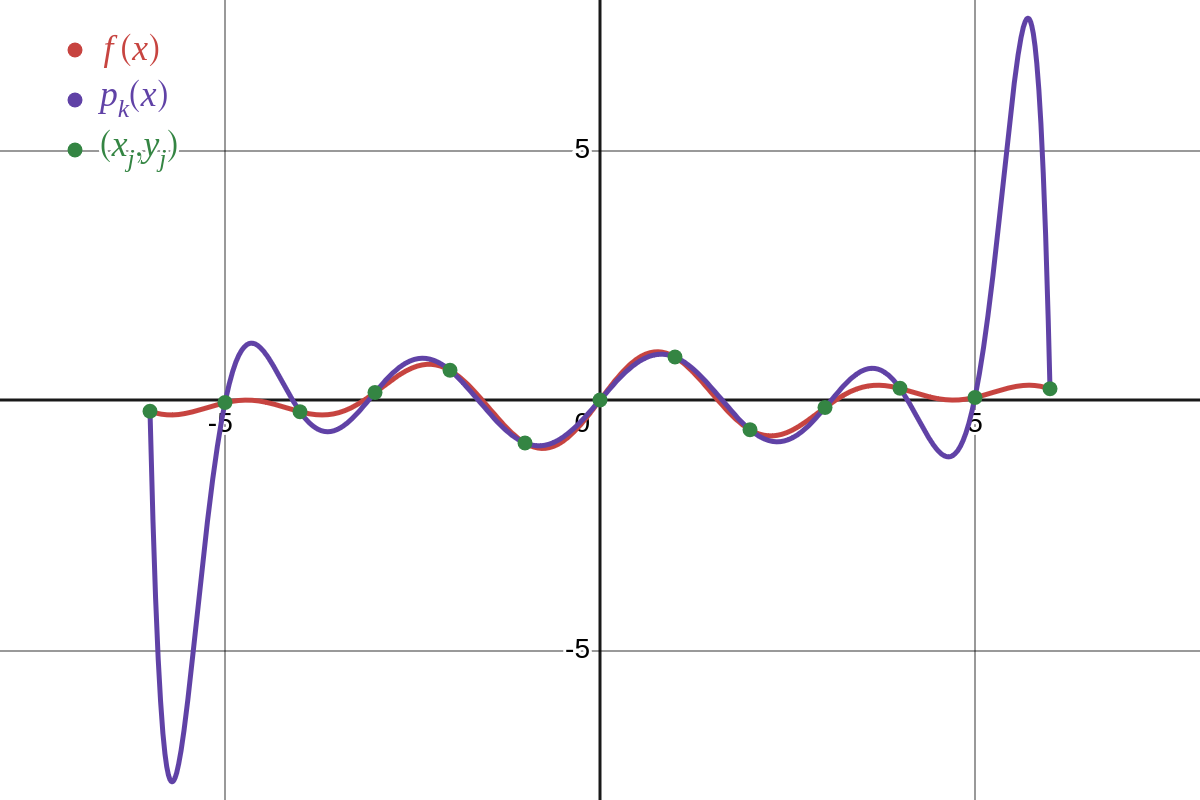
\includegraphics[scale=0.2]{../figures/lagrange_interpol.png}
	\end{center}
\end{minipage}

\subsubsection{Base di Newton}
Vediamo quindi la base di Newton, che costruiamo come:
\[
	\begin{cases}
			n_0(x) = 1 \\
			n_1(x) = x - x_0 \\
			n_2(x) = (x - x_0)(x - x_1) \\
			\vdots \\
			n_k(x) = (x - x_0) ... (x - x_{k + 1})
	\end{cases}
\]
cioè ogni $n_i$ dipende solo dai $\{ x_0, ..., x_{i - 1} \}$ precedenti.
Questo rende più facile l'aggiornamento se si aggiunge un nuovo nodo in $x_{k + 1}$, per cui basterà dire:
$$
n_{k + 1}(x) = (x - x_0) ... (x - x_k) = n_k(x) (x - x_k)
$$
Otterremo quindi la base:
$$
B_\text{Newton} = \left\{ n_0(x) = 1, n_1(x), ..., n_k(x) \right\}
$$
e la matrice di Vandermonde:
$$
V_n =
\begin{pmatrix}
	n_0(x_0) & n_1(x_0) & ... & n_k(x_0) \\ 
	\vdots & & & \vdots \\
	n_0(x_k) & n_1(x_k) & ... & n_k(x_k)
\end{pmatrix}
$$
con:
$$
p(x) = a_0 n_0(x) + a_1 n_1(x) + ... + a_k n_k(x)
$$
e nel nodo:
$$
p(x_i) = y_i \ \Leftrightarrow \ Va = y
$$
dallo svolgimento della matrice di Vandermonde si ha che la prima colonna è tutta di 1, e il resto della matrice è triangolare inferiore:
$$
V_n =
\begin{pmatrix}
	1 & 0 & ... & 0 \\
	1 & ? & ... & 0 \\
	\vdots & & & \vdots \\
	1 & ? & ... & ?
\end{pmatrix}
$$
e quindi ogni $a_i$ dipende solo dagli $\{ y_0, ... y_i \}$.
Infine, notiamo di poter scrivere ogni $a_i$ come le \textbf{differenze divise}:
$$
a_i = f[x_0, ..., x_i]
$$
indicate con le parentesi quadre, che definiamo come:
$$
f[x_0, ..., x_n, x] =
\begin{cases}
	f(x) \quad n = - 1 \\
	\frac{f(x) - f(x_0)}{x - x_0} \quad n = 0 \\
	\frac{ f[x_0, ..., x_{n - 2}, x] - f[x_0, ..., x_{n-1}, x] }{x - x_{n - 1}}, \quad \text{altrimenti}
\end{cases}
$$
cioè la serie:
$$
f[x] = f(x), \quad f[x_0, x] = \frac{f(x) - f(x_0)}{x - x_0}, \quad ...
$$

\end{document}


\documentclass[a4paper,11pt]{article}
\usepackage[a4paper, margin=8em]{geometry}

% usa i pacchetti per la scrittura in italiano
\usepackage[french,italian]{babel}
\usepackage[T1]{fontenc}
\usepackage[utf8]{inputenc}
\frenchspacing 

% usa i pacchetti per la formattazione matematica
\usepackage{amsmath, amssymb, amsthm, amsfonts}

% usa altri pacchetti
\usepackage{gensymb}
\usepackage{hyperref}
\usepackage{standalone}

% imposta il titolo
\title{Appunti Calcolo Numerico}
\author{Luca Seggiani}
\date{2025}

% disegni
\usepackage{pgfplots}
\pgfplotsset{width=10cm,compat=1.9}

% imposta lo stile
% usa helvetica
\usepackage[scaled]{helvet}
% usa palatino
\usepackage{palatino}
% usa un font monospazio guardabile
\usepackage{lmodern}

% tikz in sans
\tikzset{every picture/.style={/utils/exec={\sffamily}}}

\renewcommand{\rmdefault}{ppl}
\renewcommand{\sfdefault}{phv}
\renewcommand{\ttdefault}{lmtt}

% circuiti
\usepackage{circuitikz}
\usetikzlibrary{babel}

% disponi il titolo
\makeatletter
\renewcommand{\maketitle} {
	\begin{center} 
		\begin{minipage}[t]{.8\textwidth}
			\textsf{\huge\bfseries \@title} 
		\end{minipage}%
		\begin{minipage}[t]{.2\textwidth}
			\raggedleft \vspace{-1.65em}
			\textsf{\small \@author} \vfill
			\textsf{\small \@date}
		\end{minipage}
		\par
	\end{center}

	\thispagestyle{empty}
	\pagestyle{fancy}
}
\makeatother

% disponi teoremi
\usepackage{tcolorbox}
\newtcolorbox[auto counter, number within=section]{theorem}[2][]{%
	colback=blue!10, 
	colframe=blue!40!black, 
	sharp corners=northwest,
	fonttitle=\sffamily\bfseries, 
	title=Teorema~\thetcbcounter: #2, 
	#1
}

% disponi definizioni
\newtcolorbox[auto counter, number within=section]{definition}[2][]{%
	colback=red!10,
	colframe=red!40!black,
	sharp corners=northwest,
	fonttitle=\sffamily\bfseries,
	title=Definizione~\thetcbcounter: #2,
	#1
}

% disponi problemi
\newtcolorbox[auto counter, number within=section]{problem}[2][]{%
	colback=green!10,
	colframe=green!40!black,
	sharp corners=northwest,
	fonttitle=\sffamily\bfseries,
	title=Problema~\thetcbcounter: #2,
	#1
}

% disponi codice
\usepackage{listings}
\usepackage[table]{xcolor}

\definecolor{codegreen}{rgb}{0,0.6,0}
\definecolor{codegray}{rgb}{0.5,0.5,0.5}
\definecolor{codepurple}{rgb}{0.58,0,0.82}
\definecolor{backcolour}{rgb}{0.95,0.95,0.92}

\lstdefinestyle{codestyle}{
		backgroundcolor=\color{black!5}, 
		commentstyle=\color{codegreen},
		keywordstyle=\bfseries\color{magenta},
		numberstyle=\sffamily\tiny\color{black!60},
		stringstyle=\color{green!50!black},
		basicstyle=\ttfamily\footnotesize,
		breakatwhitespace=false,         
		breaklines=true,                 
		captionpos=b,                    
		keepspaces=true,                 
		numbers=left,                    
		numbersep=5pt,                  
		showspaces=false,                
		showstringspaces=false,
		showtabs=false,                  
		tabsize=2
}

\lstdefinestyle{shellstyle}{
		backgroundcolor=\color{black!5}, 
		basicstyle=\ttfamily\footnotesize\color{black}, 
		commentstyle=\color{black}, 
		keywordstyle=\color{black},
		numberstyle=\color{black!5},
		stringstyle=\color{black}, 
		showspaces=false,
		showstringspaces=false, 
		showtabs=false, 
		tabsize=2, 
		numbers=none, 
		breaklines=true
}

\lstdefinelanguage{javascript}{
	keywords={typeof, new, true, false, catch, function, return, null, catch, switch, var, if, in, while, do, else, case, break},
	keywordstyle=\color{blue}\bfseries,
	ndkeywords={class, export, boolean, throw, implements, import, this},
	ndkeywordstyle=\color{darkgray}\bfseries,
	identifierstyle=\color{black},
	sensitive=false,
	comment=[l]{//},
	morecomment=[s]{/*}{*/},
	commentstyle=\color{purple}\ttfamily,
	stringstyle=\color{red}\ttfamily,
	morestring=[b]',
	morestring=[b]"
}

% disponi sezioni
\usepackage{titlesec}

\titleformat{\section}
	{\sffamily\Large\bfseries} 
	{\thesection}{1em}{} 
\titleformat{\subsection}
	{\sffamily\large\bfseries}   
	{\thesubsection}{1em}{} 
\titleformat{\subsubsection}
	{\sffamily\normalsize\bfseries} 
	{\thesubsubsection}{1em}{}

% disponi alberi
\usepackage{forest}

\forestset{
	rectstyle/.style={
		for tree={rectangle,draw,font=\large\sffamily}
	},
	roundstyle/.style={
		for tree={circle,draw,font=\large}
	}
}

% disponi algoritmi
\usepackage{algorithm}
\usepackage{algorithmic}
\makeatletter
\renewcommand{\ALG@name}{Algoritmo}
\makeatother

% disponi numeri di pagina
\usepackage{fancyhdr}
\fancyhf{} 
\fancyfoot[L]{\sffamily{\thepage}}

\makeatletter
\fancyhead[L]{\raisebox{1ex}[0pt][0pt]{\sffamily{\@title \ \@date}}} 
\fancyhead[R]{\raisebox{1ex}[0pt][0pt]{\sffamily{\@author}}}
\makeatother

\begin{document}

% sezione (data)
\section{Lezione del 11-04-25}

% stili pagina
\thispagestyle{empty}
\pagestyle{fancy}

% testo
Riprendiamo il discorso dell'interpolazione polinomiale nella prospsettiva di arrivare all'interpolazione di Newton, a cui abbiamo accennato alla scorsa lezione.

Avevamo detto di avere $(x_0, y_0), (x_1, y_1), ..., (x_k, y_k)$, cioè $k + 1$ punti \textbf{distinti}, cioè con $x_i \neq x_j$, $\forall i \neq j$, tali per cui volevamo interpolarli con un polinomio di grado $k$.
Questo esisteva ed era unico appunto sotto l'ipotesi di punti distinti.


Avevamo qiundi visto le possibili base per la realizzazione di tale polinomio, di \textit{Vandermonde} e di \textit{Lagrange}.

\subsection{Differenze divise}
Avevamo poi introdotto la base di \textbf{Newton}, che definiva il polinomio del tipo:
$$
p_k (x) = \sum_{j = 0}^k a_j n_j(x) = \sum_{j = 0}^k f [ x_0, ..., x_j ] n_j(x)
$$
con:
\[
	\begin{cases}
			n_0(x) = 1 \\
			n_1(x) = x - x_0 \\
			n_2(x) = (x - x_0)(x - x_1) \\
			\vdots \\
			n_k(x) = (x - x_0) ... (x - x_{k + 1})
	\end{cases}
\]

Per la precisione, eravamo rimasti in attesa di definire i coefficienti $a_j$ del polinomio interpolante.

\par\smallskip

Cerchiamo di trovarli sfruttando la matrice di Vandermonde generalizzata (definizione 13.1):
$$
V = 
\begin{pmatrix}
	n_0(x_0) & n_1(x_0) & n_2(x_0) & ... & n_k(x_0) \\
	n_0(x_1) & n_1(x_1) & n_2(x_1) & ... & n_k(x_1) \\
	n_0(x_2) & n_1(x_2) & n_2(x_2) & ... & n_k(x_2) \\
	\vdots & & & & \vdots \\
	n_0(x_k) & n_1(x_k) & n_2(x_k) & ... & n_k(x_k) \\
\end{pmatrix}
$$
Applicando la definizione di base di Newton, si ottiene una forma del tipo:
$$
= \begin{pmatrix}
	1 & 0 & &  & ...0 \\ 
	1 & x_1 - x_0 & 0 & & ...0 \\ 
	1 & x_2 - x_0 & (x_2 - x_0)(x_2 - x_1) & 0 & ...0 \\ 
	\vdots & & & & \vdots \\
	1 & x_k - x_0 & (x_k - x_0)(x_k - x_1) & ... & (x_k - x_0) (x_k - x_1) ... (x_k - x_{k - 1}) \\ 
\end{pmatrix}
$$
cioè triangolare inferiore, e quindi risolvibile per sostituzione in avanti, imponendo:
$$
Va = y \, \Leftrightarrow \,
V \begin{pmatrix}
	a_0 \\ a_1 \\ a_2 \\ \vdots \\ a_k
\end{pmatrix}
=
\begin{pmatrix}
	y_0 \\ y_1 \\ y_2 \\ \vdots \\ y_k
\end{pmatrix}
$$

Svolgendo un paio di passaggi sella sostituzione in avanti, si ha:
\[
	\begin{cases}
		a_0 = y_0 \\
		y_0 + a_1 (x_1 - x_0) = y_1 \implies a_1 = \frac{y_1 - y_0}{x_1 - x_0} \\
		y_0 + (x_2 - x_0) \frac{y_1 - y_0}{x_1 - x_0} + (x_2 - x_0)(x_2 - x_1) a_2 = y_2 \implies a_2 = \frac{ \frac{y_2 - y_0}{x_2 - x_0} - \frac{y_1 - y_0}{x_1 - x_0} }{x_2 - x_1}
	\end{cases}
\]

Cioè si nota una forma comune per i coefficienti $a_j$

\par\smallskip

Questi coefficienti, che indichiamo con $a_j = f[x_0, ..., x_j]$ $\forall j$ si definiscono quindi per \textit{ricorsione}, e prendono il nome \textbf{differenze divise}.
Definiamo quindi la formula di ricorrenza:
\begin{definition}{Differenza divisa}
	Data una funzione $f: \mathbb{R} \rightarrow \mathbb{R}$, e dati $x_0, ..., x_{k - 1} \in \mathbb{R}$, con $x_i \neq x_j \, \forall i \neq j$, vogliamo una funzione $f[x]$ che rispetti:
	\[
		\begin{cases}
			f[x] = f(x), \quad k = 0 \\ \\
			f[x_0, x] = \frac{f(x) - f(x_0)}{x - x_0}, \quad k = 1 \\ \\
			f[x_0, x_1, x] = \frac{ \frac{f(x) - f(x_0)}{x - x_0} - \frac{f(x_1) - f(x_0)}{x_1 - x_0} }{x - x_1}, \quad k = 2 \\ \\
			f[x_0, ... , x_{k - 1}, x] = \frac{ f[x_0, ..., x] - f[x_0, ..., x_{k - 1}] }{ x - x_{k - 1} }, \quad \text{altrimenti}
		\end{cases}
	\]
	Chiamiamo questa funzione differenza divisa e la indichiamo come $f[x_0, ..., x ]$.
\end{definition}

Le differenze divise ricordano la forma del \textit{rapporto incrementale}, e anzi corrispondono esattamente a questo per $k = 1$, mentre per $k>1$ si può pensare ad un'approssimazione \textit{"grezza"}, o meglio \textit{finita},  delle derivate di ordine $k$, cioè:
\[
	\begin{cases}
		k = 0 : \quad f[x] = f(x)  \\
		k = 1 : \quad f[x_0, x] = \frac{f(x) - f(x_0)}{x - x_0} \approx \frac{df}{dx}(x_0) \\
		k = \ ? : \quad f[x_0, ... x_{k - 1}, x] = \frac{ f[x_0, ..., x] - f[x_0, ..., x_{k - 1}] }{ x - x_{k - 1} } \approx \frac{d^{k-2}f}{dx^{k-2}}(x_0) 
	\end{cases}
\]

\subsubsection{Proprietà delle differenze divise}
Possiamo trovare le seguenti proprietà delle differenze divise:
\begin{enumerate}
	\item $\forall P$ permutazione $\{i_0, ..., i_k\}$ di $\{0, ..., k \}$ vale:
		$$
			f[x_0, x_1, ..., x_k] = f[x_{i_0}, x_{i_1}, ..., x_{i_k}]
		$$
		cioè una permutazione dei $0, ..., k$ non cambia la differenza divisa;

	\item $f[x_0, ..., x_{k - 1}, x]$ è una funzione non definita in $x_0, ..., x_{k-1}$.
		Tuttavia, se $f \in C^1(I)$ con $I$ contenente $x_0, ..., x_k$, allora è prolungabile per continuità su tale intervallo;

	\item Se $f$ è non solo $C^1$, ma $f \in C^k(I)$, allora esiste $\epsilon$ tale che:
		$$
		\epsilon \in \left[ \min_{0 \leq i \leq k} x_i, \max_{0 \leq i \leq k} x_i \right]
		$$
		tale che:
		$$
		f[x_0, ..., x_k] = \frac{f^{(k)} (\epsilon) }{ k! } 
		$$ 
		Questa è una conseguenza del teorema di Lagrange.
\end{enumerate}

\subsubsection{Calcolo delle differenze divise}
Esiste un metodo piuttosto schematico per il calcolo delle differenze divise.
Dati $k + 1$ punti di interpolazione, si possono calcolare le differenze divise fino all'ordine $k$ secondo questo schema (posto $k = 3$), detto \textbf{quadro delle differenze divise}:

\begin{table}[H]
	\center 
	\begin{tabular} { c | c | p{2cm}  p{2cm} p{2cm} }
		$x$ & $f(x)$ & DD1 & DD2 & DD3 \\
		\hline
		$x_0$ & $f(x_0)$ & // & // & // \\
		$x_1$ & $f(x_1)$ & $f[x_0, x_1]$ & // & // \\
		$x_2$ & $f(x_2)$ & $f[x_0, x_2]$ & $f[x_0, x_1, x_2]$ & // \\
		$x_3$ & $f(x_3)$ & $f[x_0, x_3]$ & $f[x_0, x_2, x_3]$ & $f[x_0, x_1, x_2, x_3]$ \\
	\end{tabular}
\end{table}

Cioè a ogni passaggio completiamo una riga, da sinistra verso destra, con le differenze divise note a quel passaggio.
Notiamo che in verità le differenze divise che si trovano sulla diagonale sono le sole che compaiono effettivamente nel polinomio di Newton.

Supponendo di scrivere gli elementi della tabella come le entrate di una matrice $A = a{ij}$ triangolare inferiore, per calcolare una sua entrata $a_{ij}$ la formula da applicare è la seguente:
$$
a_{ij} = \frac{a_{i, j - 1} - a_{j - 1, j - 1}}{x_i - x}
$$

Poniamo infatti $A$:
$$
A = 
\begin{pmatrix}
	f(x_0) & & ... & & 0 \\
	f(x_1) & f[x_0, x_1] & & & & \\
	\vdots & f[x_0, x_2] & f[x_0, x_1, x_2] & & \vdots \\
	\vdots & \vdots & \vdots & & & \\
	f(x_k) &  f[x_0, x_k] & f[x_0, x_1, x_k] & ... & f[x_0, x_1, ..., x_k] \\
\end{pmatrix}
$$

\subsubsection{Esempio: quadro delle differenze divise}
Vediamo un caso pratico di quadro risolto:
\begin{table}[H]
	\center 
	\begin{tabular} { c | c | p{1cm}  p{1cm} p{1cm} }
		$x$ & $f(x)$ & DD1 & DD2 & DD3 \\
		\hline
		$0 $ & $ 3 $ & $ // $ & $ // $ & $ // $ \\
		$1 $ & $ 8 $ & $ 5 $ & $ // $ & $ // $ \\ 
		$2 $ & $ 15 $ & $ 6 $ & $ 1 $ & $ // $ \\
		$3 $ & $ 17 $ & $ 11 $ & $ 2 $ & $\frac{1}{2}$ \\
	\end{tabular}
\end{table}

A questo punto il polinomio sarà:
$$
p_3(x)
$$
$$
= f[x_0] + f[x_0, x_1] (x - x_0) + f[x_0, x_1, x_2] (x - x_0) (x - x_1) + f[x_0, x_1, x_2, x_3] (x - x_0) (x - x_1) (x - x_2) 
$$
$$
= 3 + 5 ( x - 0 ) + 1 ( x - 0 ) ( x - 1 ) + \frac{1}{2} ( x - 0 ) ( x - 1 ) ( x - 2 ) = \frac{1}{2}x^3 - \frac{1}{2}x^2 + 5x + 3
$$

Osserviamo che, nel caso in cui gli elementi di una colonna delle differenze divise siano tutti uguali, gli elementi delle colonne successive sono tutti nulli, e in particolare il grado del polinomio di interpolazione $p_k$ sarà $p_i$ con $i$ l'ultima colonna non nulla (cioè l'ordine dell'ultima differenza divisa non nulla). 

\subsubsection{Esempio: colonne nulle nel quadro}
Vediamo ad esempio il quadro delle differenze divise dove troviamo la situazione:
\begin{table}[H]
	\center 
	\begin{tabular} { c | c | p{1cm}  p{1cm} p{1cm} p{1cm} }
		$x$ & $f(x)$ & DD1 & DD2 & DD3 & DD4\\
		\hline
		$0 $ & $ 5 $ & $ // $ & $ // $ & $ // $ & $ // $ \\
		$-1 $ & $ 3 $ & $ 2 $ & $ // $ & $ // $ & $ // $ \\
		$2 $ & $ 3 $ & $ -1 $ & $ -1 $ & $ // $ & $ // $ \\
		$-2 $ & $ -9 $ & $ 7 $ & $-5 $ & $ 1 $ & $ // $ \\
		$3 $ & $ 11 $ & $ 2 $ & $ 0 $ & $ 1 $ & $ 0 $
	\end{tabular}
\end{table}

Come vediamo, alla colonna DD3 le differenze divise sono 1 e 1, ergo la differenza divisa in DD4 è nulla.
Questo significherà che il polinomio interpolante, sebbene sono stati presi $k + 1 = 5$ punti, da cui ci aspetteremo un polinomio di grado $k = 4$, ha invece grado $3$, cioè è:
$$
p_2(x) = 5 + 2 (x - 0) - 1 (x - 0)(x + 1) + 1 (x - 0)(x + 1)(x - 2) = x^3 - 2x^2 - x + 5
$$

\par\smallskip

Osserviamo infine che data una tabella di valori $(x_0, y_0), ..., (x_k, y_k)$ da interpolare, possiamo riordinarli come vogliamo nel quadro delle differenze divise.
Questo può essere utile a semplificare i calcoli.

\subsubsection{Esempio: riordinamento dei valori}
Poniamo di avere i seguenti dati:
\begin{table}[H]
	\center 
	\begin{tabular} { c | c }
		$x$ & $f(x)$ \\
		\hline
		0 & 2 \\
		1 & 1 \\
		$\alpha$ & 4 \\
		-1 & $3 \alpha + 1$ \\
		3 & 11 
	\end{tabular}
\end{table}
con $\alpha \in \mathbb{R} \setminus \{ 0, 1, -1, 3 \}$ e di chiederci quale deve essere il valore di $\alpha$ perché il polinomio interpolante abbia grado minimo.

Vediamo quindi di riordinare i dati in modo che i termini dipendenti da $\alpha$ vadano a finire in fondo alla tabella:
\begin{table}[H]
	\center 
	\begin{tabular} { c | c | p{1cm} p{1cm} p{1cm} p{1cm} }
		$x$ & $f(x)$ & DD1 & DD2 & DD3 & DD4\\
		\hline
		$0 $ & $ 2 $ & $ // $ & $ // $ & $ // $ & $ // $ \\
		$1 $ & $ 1 $ & $ -1 $ & $ // $ & $ // $ & $ // $ \\
		$3 $ & $ 11 $ & $ 3 $ & $ 2 $ & $ ...$ & $...$ \\
		$-1$ & $3 \alpha + 1$ & $1 - 3 \alpha$ & $\frac{3 \alpha - 2}{2}$ & $...$ & $...$ \\
		$\alpha$ & $4$ & $\frac{2}{\alpha}$ & $\frac{2 + \alpha}{\alpha(\alpha - 1)}$ & $...$ & $...$
	\end{tabular}
\end{table}

Alla colonna DD1 non abbiamo speranza di soddisfare la condizione di colonna tutta uguale (ci sono -1 e 3), mentre alla colonna DD2 possiamo provare ad imporre:
\[
	\begin{cases}
		\frac{3 \alpha - 2}{2} = 2 \implies \alpha = 2 \\
		\frac{2 + \alpha}{\alpha(\alpha - 1)} = 2 \implies \alpha = 2
	\end{cases}
\]
che quindi, per pura fortuna, corrisponde.
Possiamo allora prendere $\alpha = 2$ e completare il quadro:
\begin{table}[H]
	\center 
	\begin{tabular} { c | c | p{1cm} p{1cm} p{1cm} p{1cm} }
		$x$ & $f(x)$ & DD1 & DD2 & DD3 & DD4\\
		\hline
		$0 $ & $ 2 $ & $ // $ & $ // $ & $ // $ & $ // $ \\
		$1 $ & $ 1 $ & $ -1 $ & $ // $ & $ // $ & $ // $ \\
		$3 $ & $ 11 $ & $ 3 $ & $ 2 $ & $ // $ & $ // $ \\
		$-1$ & $3 \alpha + 1$ & $1 - 3 \alpha$ & $2$ & $0$ & $ // $ \\
		$\alpha$ & $4$ & $\frac{2}{\alpha}$ & $2$ & $0$ & $0$
	\end{tabular}
\end{table}
da cui il polinomio al solo grado 2:
$$
p_2(x) = 2 - x + 2x(x - 1) = 2x^2 - 3x + 2
$$

\subsubsection{Esempio: interpolazione di Newton}
A scopo di esempio, vediamo l'interpolazione di Newton della funzione:
$$
f\left(x\right)=\frac{x^{3}}{30}-\cos\left(\frac{3}{2}x\right)\ 
$$
Approssimata secondo la tabella di nodi:
\begin{table}[H]
	\center
	\begin{tabular} { c | p{1cm} p{1cm} p{1cm} p{1cm} p{1cm} p{1cm} p{1cm} }
		$x_j$ & $-5$ & $-4$ & $-1.9$ & $0$ & $2.3$ & $3.5$ & $5$ \\
		$y_j$ & $-4.51$ & $-3.09$ & $0.73$ & $-1$ & $1.36$ & $0.92$ & $3.82$
	\end{tabular}
\end{table}

Il polinomio si trova quindi prendendo le basi di Newton $n_j(x)$ e calcolando le differenze divise, come abbiamo visto finora:

\begin{table}[H]
	\center 
	\begin{tabular} { c | c | p{1cm} p{1cm} p{1cm} p{1cm} p{1cm} p{1cm} }
		$x$ & $f(x)$ & DD1 & DD2 & DD3 & DD4 & DD5 & DD6 \\
		\hline
		$-5 $ & $ -4.51 $ & $ // $ & $ // $ & $ // $ & $ // $ & $ // $ & $ // $ \\
		$-4 $ & $ -3.09 $ & $ 1.42 $ & $ // $ & $ // $ & $ // $ & $ // $ & $ // $ \\
		$-1.9 $ & $ 0.73 $ & $ 1.69 $ & $ 0.13 $ & $ // $ & $ // $ & $ // $ & $ // $ \\
		$0 $ & $ -1 $ & $ 0.7 $ & $ -0.18 $ & $ -0.16 $ & $ // $ & $ // $ & $ // $ \\
		$2.3 $ & $ 1.36 $ & $ 0.8 $ & $ -0.1 $ & $ -0.05 $ & $ 0.05 $ & $ // $ & $ // $ \\
		$3.5 $ & $ 0.92 $ & $ 0.64 $ & $ -0.1 $ & $ -0.04 $ & $ 0.03 $ & $ -0.01 $ \\
		$5 $ & $ 3.82 $ & $ 0.83 $ & $ -0.06 $ & $ -0.03 $ & $ 0.03 $ & $ \sim0 $ & $ \sim0$ 
	\end{tabular}
\end{table}

Da cui il polinomio:

$$
p_k(x) = -4.51 n_0(x) + 1.42 n_1(x) + 0.13 n_2(x) - 0.16 n_3(x) + 0.05 n_4(x) - 0.01 n_5(x)
$$

Vediamo quindi un grafico che mostra tale polinomio, sovraimposto alla funzione originale e ai nodi campionati:

\begin{center}
	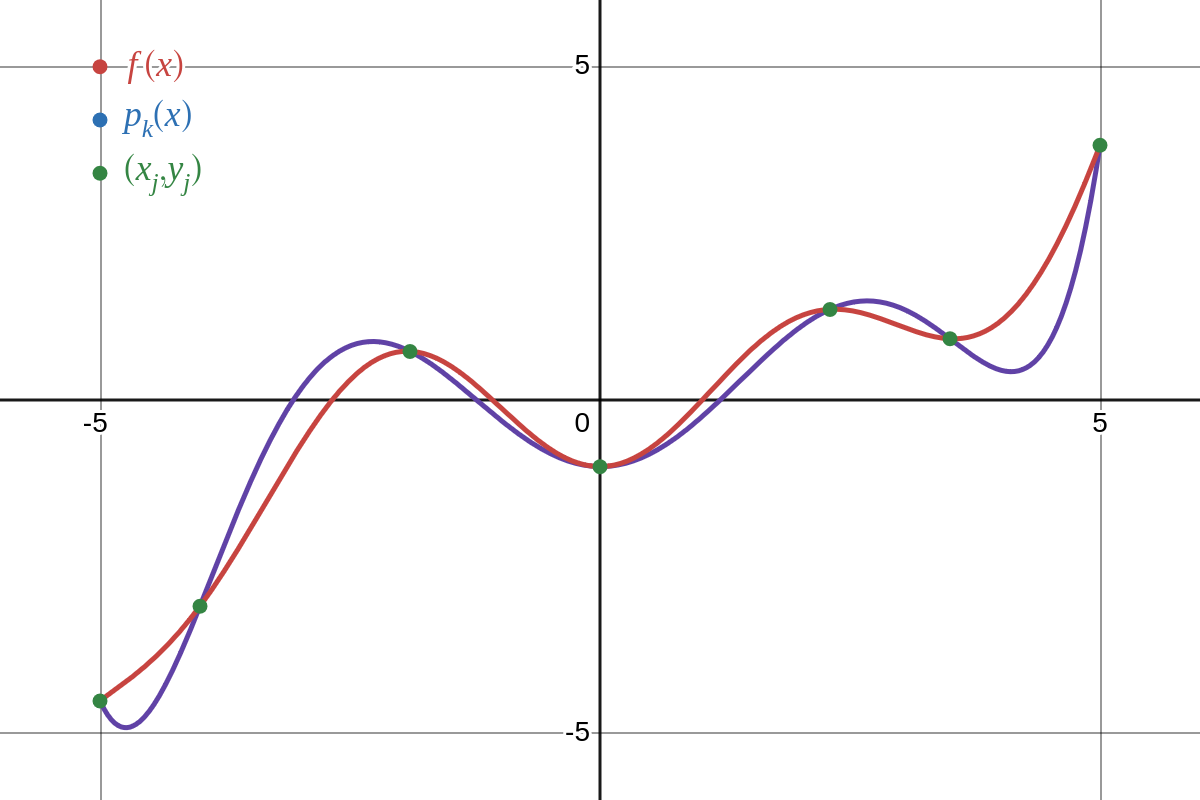
\includegraphics[scale=0.3]{../figures/newton_interpol.png}
\end{center}

Il grafico è stato realizzato con Desmos (\url{https://www.desmos.com/calculator/tavjyzgpd0}), assieme allo scorso esempio sull'interpolazione di Lagrange (\url{https://www.desmos.com/calculator/w2tx5n7jtp}, esempio 13.1.3).
Il calcolo al computer ci permette chiaramente di ottenere risultati più precisi, as esempio in questo caso a valutare il coefficiente della base di sesto grado (che svanisce approssimando alle prime 2 cifre decimali). 

\newpage

\subsection{Errore nell'approssimazione polinomiale}
Veniamo quindi alla valutazione dell'errore.
Vale il seguente teorema:
\begin{theorem}{Errore dell'approssimazione polinomiale}
	Presi $k + 1$ punti $x_0, ..., x_k$ con $x_i \neq x_j \, \forall i \neq j$.
	Sia $f: \mathbb{R} \rightarrow \mathbb{R}$ tale che $f \in C^{k + 1}(I)$ con $I \subseteq \mathbb{R}$ contenente $x_0, ..., x_k$.
	Se $p_k(x)$ è il polinomio di interpolazione di grado al più $k$ che interpola i punti $(x_0, f(x_0), ..., (x_k, f(x_k)))$ allora riguardo all'errore vale:
$$
f(x) - p_k(x) = \Pi(x) \frac{f^{(k + 1)}(\xi)}{(k + 1)!}
$$
con:
$$
\Pi(x) = \prod_{j = 0}^k (x - x_j)
$$
per un certo $\xi$ tale che:
$$
\xi \in \left[ \min_{0 \leq i \leq k} x_i \cup x, \max_{0 \leq i \leq k} x_i \cup x \right]
$$
\end{theorem}

Osserviamo quindi che conoscendo una stima di $|f^{k + 1}|$ e  di $|\Pi(x)|$ si può provare a stimare l'errore del polinomio di interpolazione quando si valuta $p_k(x)$ fuori dai nodi $\{ x_j \}_{j=0}^k$.

\subsection{Considerazioni ulteriori sull'approssimazione polinomiale}
Vediamo quindi alcune nozioni che riguardano sia l'approssimazione di Newton che quella di Lagrange, che abbiamo visto rispettivamente in 13.1.4 e 14.1, e 13.1.2 (e che riguardano in verità anche il metodo di approssimazione di Vandermonde visto in 13.1.1).

\subsubsection{Riassunto fra base di Newton e base di Lagrange}
Facciamo quindi un riassunto confrontando la base di Newton e la base di Lagrange.
\begin{table}[h!]
	\center 
	\begin{tabular} { c p{6cm} | p{6cm} }
		& \bfseries Newton & \bfseries Lagrange \\
		\hline
		\bfseries Base & $n_j(x) = (x - x_0) ... (x - x_{j - 1}) $ & $l_j(x) = \prod_{i \neq j}^k \frac{x - x_i}{x_j - x_i}$ \\
		\bfseries Coef. & $f[x_0, ... x_j]$ & $f(x_j) = y_j$ \\ & \\
		& Con la base di Newton, se si è calcolato $p_k(x)$ e si vuole $p_{k + 1}(x)$, basta calcolare $m_{k + 1}$ e $f[x_0, ..., x_{k}]$ da $f[x_0, ..., x_{k - 1}]$ &
		Con la base di Lagrange, per fare la stessa cosa bisogna ricalcolare tutti gli $e_j(x)$ \\ & \\
		& Il grado del polinomio si nota facilmente & Per trovare il grado del polinomio bisogna espandere nella base dei monomi
	\end{tabular}
\end{table}

Viene da sé che i metodi di Vandermonde, Lagrange e Newton restituiscono tutti lo stesso polinomio (se non in forma algebricamente diversa), in quanto il polinomio interpolante di grado minimo è l'unico che passa per i punti $(x_j, y_j)$ forniti.

\subsubsection{Fenomeno di Runge}
Vediamo un fenomeno che accumuna tutti i tipi di approssimazione polinomiale: presa una certa approssimazione di grado $k$ di una funzione $f(x)$, quindi un polinomio $p(x)$ passante per $k + 1$ punti campionati da $f(x)$, si potrebbe pensare che aumentando il valore di $k$ si otterrebbero approssimazioni via via più accurate.
Questo è giusto per quanto riguarda i punti interni, ma riguardo agli estremi dell'intervallo di approssimazione notiamo che la funzione di errore $r(x) = p(x) - f(x)$ ha un errore costante se non addirittura crescente al crescere di $k$.

Prendiamo ad esempio la funzione:
$$
f(x) = \frac{1}{1 + x^2} \quad \text{(versiera di Agnesi)}
$$
interpolata fra $-2$ e $2$ ad intervalli regolari, quindi preso $k$ interpolata sui nodi:
$$
x_k = -2 + \frac{4}{k}i, \quad i = 0, 1, ..., k
$$

Con $k = 4$, si ottiene il seguente polinomio interpolante:
\begin{center}
	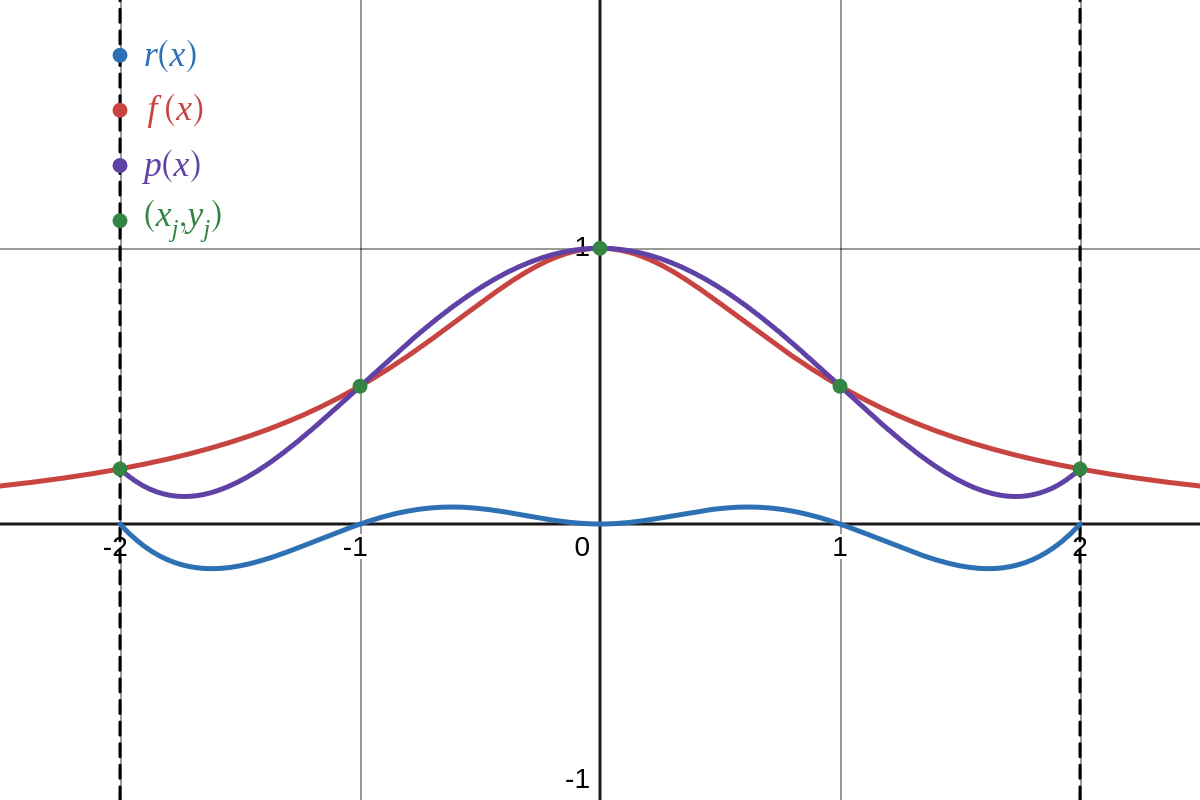
\includegraphics[scale=0.28]{../figures/runge_k4.png}
\end{center}

\newpage

Aumentando il grado a $k = 40$, quindi moltiplicando per 10, si ottiene invece il polinomio interpolante:
\begin{center}
	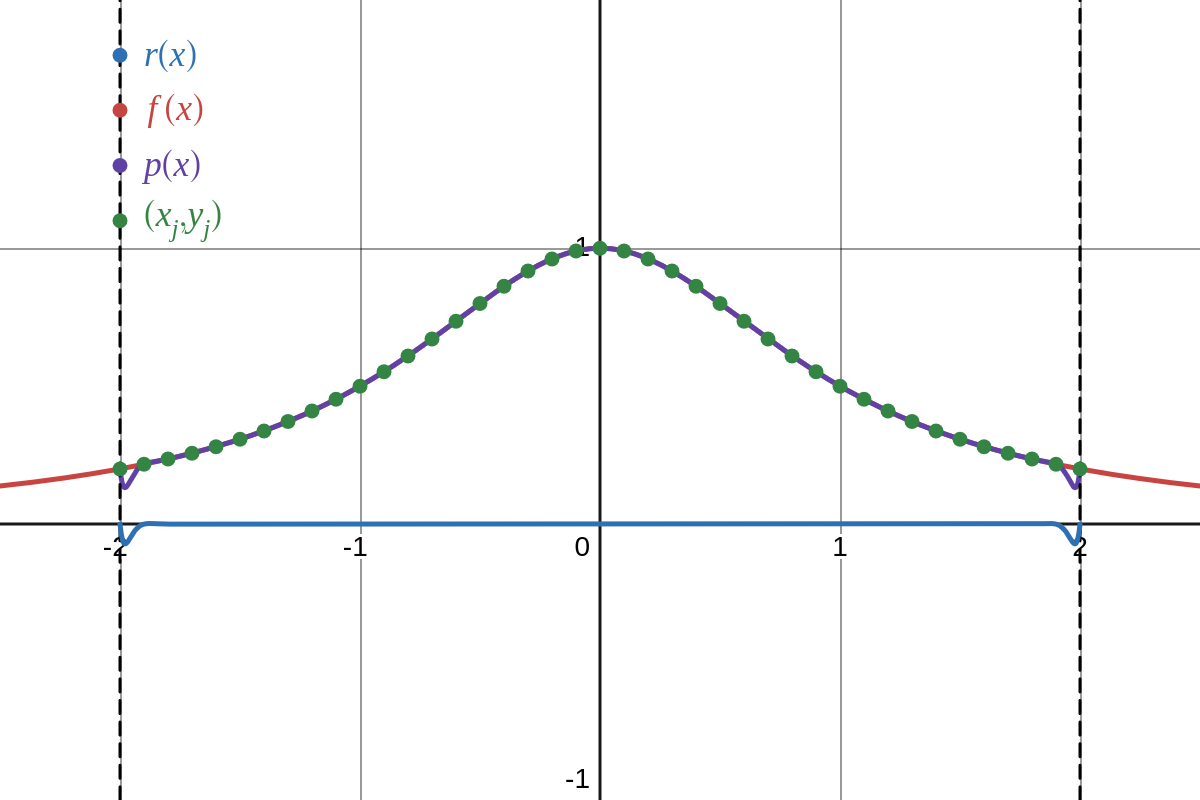
\includegraphics[scale=0.28]{../figures/runge_k40.png}
\end{center}
che è sì più accurato nei punti interni, ma ha comunque un certo errore in corrispondenza degli estremi $x = -2$ e $x = 2$.

Si può dimostrare che questo fenomeno permane al crescere di $k$, ergo aumentare il grado non corrisponde sempre a migliorare l'accuratezza dell'approssimazione.

\subsubsection{Nodi di Chebysev}
Un modo per migliorare l'accuratezza delle approssimazioni polinomiali, e sopratutto per evitare il fenomeno di Runge in prossimità degli estremi, può essere quello di cambiare i nodi presi, usando i cosiddetti \textbf{nodi di Chebyshev}.

\begin{definition}{Nodi di Chebyshev}
	Si chiamano nodi di Chebysev unitari gli $n$ punti $x_k$:
	$$
	x_k = \cos\left(\frac{\left(K+\frac{1}{2}\right)\pi}{n_{p}}\right), \quad k = 0, ..., n - 1
	$$
\end{definition}

\par\bigskip

\noindent
\begin{minipage}{\textwidth}
I nodi di Chebyshev corrispondono alle proiezioni sull'asse $x$ di punti equispaziati sulla parte superiore di una circonfenferenza unitaria, cioè sul grafico:
\begin{center}
	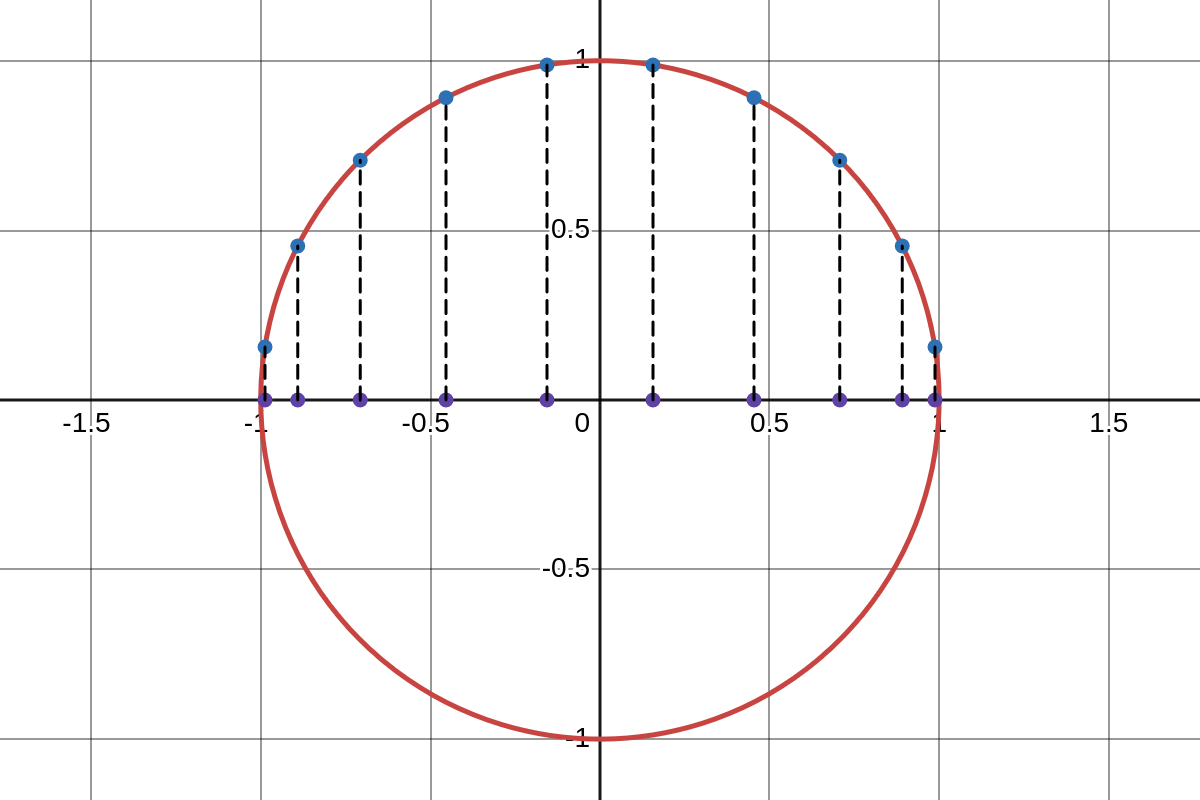
\includegraphics[scale=0.28]{../figures/chebyshev_nodes.png}
\end{center}
\end{minipage}

\par\bigskip

Utilizzando i nodi di Chebyshev nel calcolo del polinomio interpolante, si usano risultati molto più accurati.
Ad esempio, per l'approssimazione della stessa curva del paragrafo scorso, si ottiene che già con $k = 10$ il grafico ha la aspetto:
\begin{center}
	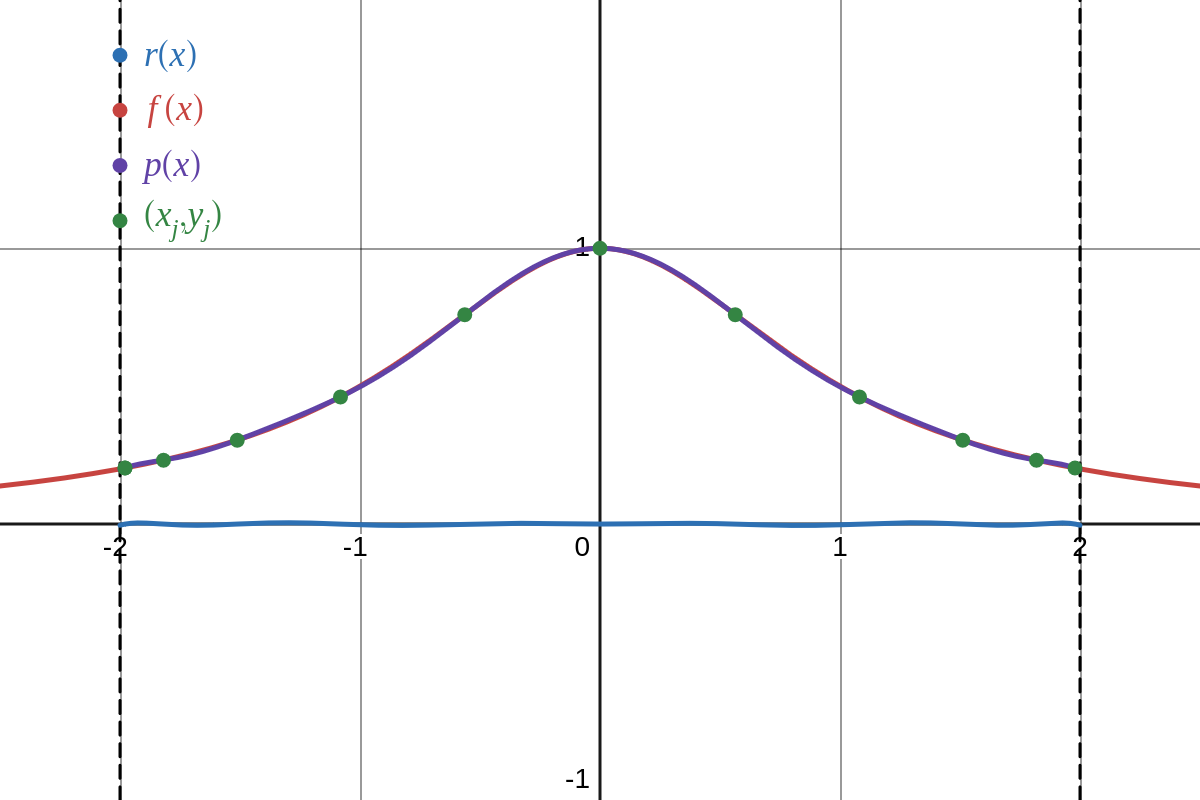
\includegraphics[scale=0.28]{../figures/runge_better.png}
\end{center}
da dove notiamo quindi che l'errore, sopratutto vicino agli estremi, è significativamente ridotto.

\subsection{Interpolazione osculatoria di Hermite}
Vediamo un altro metodo per interpolare polinomi.
Supponiamo di conoscere non soltanto ai nodi il valore della funzione, ma anche il valore della sua derivata.
In questo caso potremo costruire un polinomio in cui le valutazioni e quelle derivata equivalongono rispettivamente ai valori di $f$ e $f'$.
Questo potrebbe essere utile nel caso in cui conosciamo sia la posizione che la velocità di un corpo in certi istanti e vogliamo approssimarne la traiettoria.

Definiamo quindi:
\begin{definition}{Polinomio interpolante di Hermite }
	Dati $x_0, ..., x_k \in I \subseteq \mathbb{R}$ e $2k + 2$ valori $\{f(x_0), ..., f(x_k) \}$ e $\{ f'(x_0), ..., f'(x_k) \}$ di una certa funzione $f \in C^{1}(I)$, si dice polinomio interpolante di Hermite, per $f$ coi nodi $x_0, ..., x_k$, il polinomio $H_{2k + 1}(x)$ di grado al più $2k + 1$ tale che:
	$$
		H_{2k + 1}(x_j) = f(x_j), \quad H'_{2k + 1}(x_j) = f'(x_j), \quad \forall j = 0, ..., k
	$$
\end{definition}

Varrà quindi il seguente teorema:
\begin{theorem}{Esistenza del polinomio interpolante di Hermite}
	Se $x_i \neq x_j$ $\forall i \neq j$ allora esiste ed è unico il polinomio di Hermite $H_{2k + 1}$ per $f \in C^1(I)$. 
\end{theorem}
La dimostrazione di unicità si ha ipotizzando, per assurdo, che esista un secondo polinomio di hermite $S_{2k+1}$.
A questo punto si potrà definire la funzione di errore:
$$
R(x) = H_{2k + 1}(x) - S_{2k + 1}(x)
$$
Questà dovrà annullarsi fino al primo grado in $x_0, ..., x_k$, per cui dovrà essere divisiibile per:
$$
Q(x) = (x - x_0)^2 ... (x - x_k)^2
$$
Questo però significherebbe che $R(x)$, e quindi $H_{2k + 1}$ e $S_{2k + 1}$, dovrebbero essere almeno di grado $2k + 2$ (il grado di $Q(x)$), che viola le ipotesi. \qed 

\par\smallskip

Vediamo allora come trovare il polinomio $H_{2k + 1}$ vero e proprio.
Si potrebbe formulare un sistema lineare come è stato fatto nel caso della base canonica, che dava la matrice standard di Vandermonde.

In questo caso partiremo dall'ipotizzare riguardo a $H_{2k + 1}$:
$$
\mathrm{deg}(H_{2k + 1}) = 2k + 1, \quad H_{2k + 1} = a_0 + a_1 x + a_2 x^2 + ... + a_{2k + 1} x^{2k + 1} = \sum_{i = 0}^{2k + 1} a_i x^i
$$
e quindi imporre le condizioni:
\[
	\begin{cases}
		a_0 + a_1 x_0 + a_2 x_0^2 + ... + a_{2k + 1} x_0^{2k + 1} = f(x_0) \\	
		\vdots \\
		a_0 + a_1 x_k + a_2 x_k^2 + ... + a_{2k + 1} x_k^{2k + 1} = f(x_k) \\
		a_1 + 2 a_2 x_0 + ... + (2k + 1) a_{2k + 1} x_0^{2k} = f'(x_0) \\
		\vdots \\
		a_1 + 2 a_2 x_k + ... + (2k + 1) a_{2k + 1} x_k^{2k} = f'(x_k)
	\end{cases}
\]
da cui, volendo esprimere il sistema come $Va = y$, si ottiene la "matrice di Vandermonde":
$$
V = 
\begin{pmatrix}
	1 & x_0 & x_0^2 & ... & x_0^{2k + 1} \\	
	\vdots  & & & & \vdots \\
	1 & x_k & x_k^2 & ... & x_k^{2k + 1} \\
	0 & 1 & 2 x_0 & ... & (2k + 1) x_0^{2k} \\
	\vdots  & & & & \vdots \\
	0 & 1 & 2 x_k & ... & (2k + 1) x_k^{2k} 
\end{pmatrix}
$$

Spesso, però, questo procedimento non conviene in quanto si incontrano gli stessi problemi di malcondizionamento che avevamo incontrato anche nella matrice standard di Vandermonde.

\par\smallskip

Tipicamente allora si procede in maniera analoga all'interpolazione di Lagrange, ma generalizzata per ottenere le condizioni sulle derivate.
Più precisamente, cerchiamo un polinomio della forma:
$$
H_{2k + 1}(x) = \sum_{j = 0}^k h_{0j}(x) f(x_j) + \sum_{j = 0}^k h_{1j}(x) + f'(x_j)
$$

Avremo che $f(x_j)$ e $f'(x_j)$ sono chiaramente i dati del problema, che farano da coefficienti, mentre $h_{0j}(x)$ e $h_{1j}(x)$ saranno polinomi di grado $2k + 1$ tali che:
\begin{equation}
h_{0j}(x_i) =
\begin{cases}
	1, \quad i = j \\
	0, \quad i \neq j
\end{cases}, \quad
h'_{0j}(x_i) = 0  \quad \forall \, 0 \leq i \leq k
$$
$$
h_{1j}(x_i) = 0, \quad
h'_{1j}(x_i) =
\begin{cases}
	1, \quad i = j \\
	0, \quad i \neq j
\end{cases} \quad \forall \, 0 \leq i \leq k
\end{equation}
che possiamo interpretare come le condizioni imposte alle basi di Lagrange generalizzata al caso con la derivata prima.

Se valgono queste proprietà, infatti, si ha che:
$$
H_{2k + 1}(x_i) = \sum_{j = 0}^k h_{0j}(x_j) f(x_i) + \sum_{j = 0}^k h_{1j}(x_i) f'(x_j) = f(x_j) + 0 
$$
e rispetto alla derivata prima:
$$
H'_{2k + 1}(x_i) = \sum_{j = 0}^k h_{0j}'(x_i) f(x_j) + \sum_{j = 0}^k h'_{1j}f'(x_j) = 0 + f'(x_i)
$$
con in entrambi i casi, $\forall \, i = 0, ..., k$.

Osserviamo che come nel caso dell'interpolazione standard, stiamo rinunciando a cercare una rappresentazione di $H_{2k + 1}$ nella base dei monomi $\{ 1, x, ..., x^{2k + 1} \}$ e cerchiamo invece un'espressione rispetto alla base:
$$
	B_\text{Hermite} = \{ h_{01}(x), ..., h_{0k}(x), h_{10}(x), ..., h_{1k}(x) \}
$$
in cui i coefficienti delle combinazioni lineari sono:
$$
f(x_0), ..., f(x_k), f'(x_0), ..., f'(x_k)
$$

Il problema si riconduce quindi a trovare $h_{0j}(x)$, $h_{1j}(x)$ $\forall j$ che soddisfino le proprietà (3).

L'idea parte dall'\textit{ansatz} di cercare $h_{0j}$ e $h_{1j}$ della forma:
$$
h_{0j} = (Ax + B) e_j^2(x), \quad h_{1j} = (Cx + D) e_j^2(x)
$$
con $e_j(x)$ $j$-esimo polinomio in base di Lagrange, cioè:
$$
e_j(x) = \prod_{i \neq j}^k \frac{x - x_i}{x_j - x_i}
$$

Imponiamo quindi le proprietà (3) per ricavare $A, B, C, D$ di ogni $h_{0j}$ e $h_{1j}$.
\begin{itemize}
	\item $h_{0j}(x)$: avremo che la proprietà di grado zero è sempre rispettata finché:
		$$
		A x_j + B = 1
		$$
		in quanto $e_j^2(x_j)$ vale 1 o 0 esattamente come richiesto.
		Riguardo al primo grado, avremo invece:
		$$
		h_{0j}'(x_j) = A e_j^2 (x_j) + 2 (A x_j + B) e_j(x_j) e_j'(x_j) = 0
		$$
		dove si possono eliminare i termini $A x_j + B$ e $e_j(x_j)$, e quindi:
		$$
		A + 2 e_j'(x_j) = 0 \implies A = - 2 e_j'(x_j) 
		$$
		sostituendo in $Ax_j + B$ si trova allora:
		$$
		B = 1-2 e_j'(x_j) x_j
		$$
		da cui la funzione finale:
		$$
		h_{0j} = \left( 1 - 2 e_j'(x_j) (x - x_j) \right) e_j^2(x)
		$$

	\item $h_{1j}(x)$: avremo che la proprietà di grado zero è sempre rispettata finché:
		$$
		C x_j + D = 0
		$$
		in quanto $e_j^2(x_j)$ vale 1 soltanto in $x_j$, e lì vogliamo annullarlo.
		Riguardo al primo grado, avremo invece:
		$$
		h_{1j}' (x) = C e_j^2 (x) + 2 (Cx + D) e_j(x) e'_j(x) = 1
		$$
		dove si possono fare le stesse semplificazioni di sopra, e quindi:
		$$
		h_{1j}' = C e_j^2(x) \implies C = 1
		$$
		sostituendo in $Cx_j + D$ si trova allora:
		$$
		D = - x_j
		$$
		da cui la funzione finale:
		$$
		h_{1j}(x) = (x - x_j) e^2_j(x)
		$$
\end{itemize}

Abbiamo quindi ottenuto le due funzioni $h_{0j}$ e $h_{1j}$:
\[
	\begin{cases}
		h_{0j}(x) = \left( 1 - 2 e_j'(x_j) (x - x_j) \right) e_j^2(x) \\
		h_{1j}(x) = (x - x_j) e^2_j(x)
	\end{cases}
\]
ossia il polinomio interpolante di Hermite avrà la forma:
$$
H_{2k + 1}(x) = \sum_{j = 0}^k f(x_j) \left( 1 - 2 e_j'(x_j)(x - x_j) \right) e_j^2(x) + \sum_{j = 0}^k f'(x_j) (x - x_j) e_j^2(x)
$$

\subsubsection{Esempio: raccordo di binari}
Supponiamo di avere 2 binari e di volerli unire in maniera $C^1$, ovvero di voler trovare un polinomio $H_3(x)$ tale che:
\[
	\begin{cases}
		H_3(0) = 0 \\
		H_3(d) = L
	\end{cases}, \quad
	\begin{cases}
		H_3'(0) = 0 \\
		H_3'(d) = S
	\end{cases} 
\]

Il polinomio dovrà essere di grado 3 (le due condizioni alle derivate contano nel calcolo del grado).
Dobbiamo calcolare, prima di tutto, le basi di Lagrange:
$$
e_0(x) = \frac{x - d}{d}, \quad e_1(x) = \frac{x}{d}
$$
e sostituire quindi nelle formule per $h_{0j}(x)$ e $h_{1j}(x)$:
$$
h_{00}(x) = \left( 1 + 2\frac{x}{d} \right) \frac{(x - d)^2}{d^2}, \quad h_{01}(x) = \left( 1 - 2 \frac{x - d}{d} \right) \frac{x^2}{d^2}
$$
$$
h_{10}(x) = x \frac{(x - d)^2}{d^2}, \quad h_{11} = (x - d) \frac{x^2}{d^2}
$$
per cui otterremo:
$$
H_3(x) = 0 \cdot h_{00}(x) + L \cdot h_{01}(x) + 0 \cdot h_{10}(x) + S \cdot h_{11}(x) = L \left( 1 - 2 \frac{x - d}{d} \right) \frac{x^2}{d^2} + S (x - d) \frac{x^2}{d^2}
$$

Vediamo un esempio grafico:
\begin{center}
	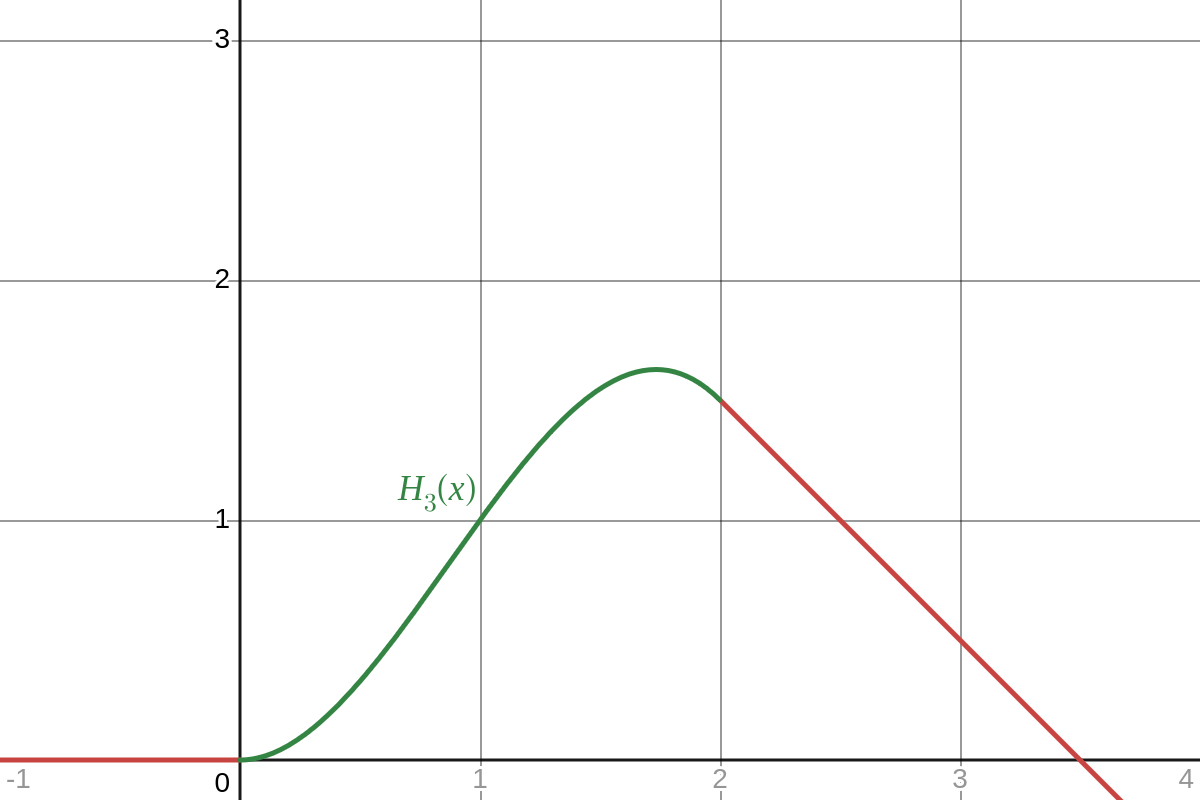
\includegraphics[scale=0.28]{../figures/tracks.png}
\end{center}

\subsubsection{Errore nell'approssimazione di Hermite}
Valutiamo quindi l'errore:
\begin{theorem}{Errore dell'approssimazione di Hermite}
	Data $f \in C^{2k + 2}(I)$ allora:
$$
f(x) - H_{2k + 1}(x) = \Pi^2 (x) \frac{f^{(2k + 1)(\xi)}}{(2k + 2)!}
$$
con le stesse definizioni del 14.1.
\end{theorem}

\end{document}


\documentclass[a4paper,11pt]{article}
\usepackage[a4paper, margin=8em]{geometry}

% usa i pacchetti per la scrittura in italiano
\usepackage[french,italian]{babel}
\usepackage[T1]{fontenc}
\usepackage[utf8]{inputenc}
\frenchspacing 

% usa i pacchetti per la formattazione matematica
\usepackage{amsmath, amssymb, amsthm, amsfonts}

% usa altri pacchetti
\usepackage{gensymb}
\usepackage{hyperref}
\usepackage{standalone}

% imposta il titolo
\title{Appunti Calcolo Numerico}
\author{Luca Seggiani}
\date{2025}

% disegni
\usepackage{pgfplots}
\pgfplotsset{width=10cm,compat=1.9}

% imposta lo stile
% usa helvetica
\usepackage[scaled]{helvet}
% usa palatino
\usepackage{palatino}
% usa un font monospazio guardabile
\usepackage{lmodern}

% tikz in sans
\tikzset{every picture/.style={/utils/exec={\sffamily}}}

\renewcommand{\rmdefault}{ppl}
\renewcommand{\sfdefault}{phv}
\renewcommand{\ttdefault}{lmtt}

% circuiti
\usepackage{circuitikz}
\usetikzlibrary{babel}

% disponi il titolo
\makeatletter
\renewcommand{\maketitle} {
	\begin{center} 
		\begin{minipage}[t]{.8\textwidth}
			\textsf{\huge\bfseries \@title} 
		\end{minipage}%
		\begin{minipage}[t]{.2\textwidth}
			\raggedleft \vspace{-1.65em}
			\textsf{\small \@author} \vfill
			\textsf{\small \@date}
		\end{minipage}
		\par
	\end{center}

	\thispagestyle{empty}
	\pagestyle{fancy}
}
\makeatother

% disponi teoremi
\usepackage{tcolorbox}
\newtcolorbox[auto counter, number within=section]{theorem}[2][]{%
	colback=blue!10, 
	colframe=blue!40!black, 
	sharp corners=northwest,
	fonttitle=\sffamily\bfseries, 
	title=Teorema~\thetcbcounter: #2, 
	#1
}

% disponi definizioni
\newtcolorbox[auto counter, number within=section]{definition}[2][]{%
	colback=red!10,
	colframe=red!40!black,
	sharp corners=northwest,
	fonttitle=\sffamily\bfseries,
	title=Definizione~\thetcbcounter: #2,
	#1
}

% disponi problemi
\newtcolorbox[auto counter, number within=section]{problem}[2][]{%
	colback=green!10,
	colframe=green!40!black,
	sharp corners=northwest,
	fonttitle=\sffamily\bfseries,
	title=Problema~\thetcbcounter: #2,
	#1
}

% disponi codice
\usepackage{listings}
\usepackage[table]{xcolor}

\definecolor{codegreen}{rgb}{0,0.6,0}
\definecolor{codegray}{rgb}{0.5,0.5,0.5}
\definecolor{codepurple}{rgb}{0.58,0,0.82}
\definecolor{backcolour}{rgb}{0.95,0.95,0.92}

\lstdefinestyle{codestyle}{
	backgroundcolor=\color{black!5}, 
	commentstyle=\color{codegreen},
	keywordstyle=\bfseries\color{magenta},
	numberstyle=\sffamily\tiny\color{black!60},
	stringstyle=\color{green!50!black},
	basicstyle=\ttfamily\footnotesize,
	breakatwhitespace=false,         
	breaklines=true,                 
	captionpos=b,                    
	keepspaces=true,                 
	numbers=left,                    
	numbersep=5pt,                  
	showspaces=false,                
	showstringspaces=false,
	showtabs=false,                  
	tabsize=2
}

\lstdefinestyle{shellstyle}{
	backgroundcolor=\color{black!5}, 
	basicstyle=\ttfamily\footnotesize\color{black}, 
	commentstyle=\color{black}, 
	keywordstyle=\color{black},
	numberstyle=\color{black!5},
	stringstyle=\color{black}, 
	showspaces=false,
	showstringspaces=false, 
	showtabs=false, 
	tabsize=2, 
	numbers=none, 
	breaklines=true
}

\lstdefinelanguage{javascript}{
	keywords={typeof, new, true, false, catch, function, return, null, catch, switch, var, if, in, while, do, else, case, break},
	keywordstyle=\color{blue}\bfseries,
	ndkeywords={class, export, boolean, throw, implements, import, this},
	ndkeywordstyle=\color{darkgray}\bfseries,
	identifierstyle=\color{black},
	sensitive=false,
	comment=[l]{//},
	morecomment=[s]{/*}{*/},
	commentstyle=\color{purple}\ttfamily,
	stringstyle=\color{red}\ttfamily,
	morestring=[b]',
	morestring=[b]"
}

% disponi sezioni
\usepackage{titlesec}

\titleformat{\section}
{\sffamily\Large\bfseries} 
{\thesection}{1em}{} 
\titleformat{\subsection}
{\sffamily\large\bfseries}   
{\thesubsection}{1em}{} 
\titleformat{\subsubsection}
{\sffamily\normalsize\bfseries} 
{\thesubsubsection}{1em}{}

% disponi alberi
\usepackage{forest}

\forestset{
	rectstyle/.style={
		for tree={rectangle,draw,font=\large\sffamily}
	},
	roundstyle/.style={
		for tree={circle,draw,font=\large}
	}
}

% disponi algoritmi
\usepackage{algorithm}
\usepackage{algorithmic}
\makeatletter
\renewcommand{\ALG@name}{Algoritmo}
\makeatother

% disponi numeri di pagina
\usepackage{fancyhdr}
\fancyhf{} 
\fancyfoot[L]{\sffamily{\thepage}}

\makeatletter
\fancyhead[L]{\raisebox{1ex}[0pt][0pt]{\sffamily{\@title \ \@date}}} 
\fancyhead[R]{\raisebox{1ex}[0pt][0pt]{\sffamily{\@author}}}
\makeatother

\begin{document}

% sezione (data)
\section{Lezione del 14-04-25}

% stili pagina
\thispagestyle{empty}
\pagestyle{fancy}

% testo
Abbiamo finora presupposto di avere una serie di punti $(x_j, y_j)$, con $j = 0, ..., k$, tratti da una funzione $f : [a, b] \rightarrow \mathbb{R}$, cioè definita su un certo intervallo $[a, b]$, con $x_j \in [a, b]$ e $y_j = f(x_j) \in \mathbb{R}$.
Da questi punti volevamo ricavare un polinomio $p(x)$ di grado al più $k$ tale che questo interpolasse i punti, cioè verificasse:
$$
p(x_j) = y_j
$$

Da questa configurazione avevamo visto più metodi per il calcolo effettivo di $p(x)$, e avevamo ipotizzato che il modo migliore per aumentarne l'accuratezza, cioè ridurre il massimo della funzione:
$$
r(x) = f(x) - p(x), \quad x \in [a, b]
$$
fosse aumentare $k$.

Questo però aveva diversi aspetti negativi:
\begin{itemize}
	\item Avere $k$ maggiore significa aumentare i punti campionati, cosa che potrebbe non essere sempre fattibile;
	\item Non è detto che $k$ maggiore aumenti l'accuratezza: avevamo visto infatti il \textit{fenomeno di Runge} agli estremi, per cui il limiter dell'errore all'aumentare di $k$ non era zero, cioè:
		$$
		\lim_{k \rightarrow +\infty} |r(x)| \neq 0
		$$
		Avevamo visto un modo per migliorare questa situazione, che era usare nodi non equispaziati ma equispaziati su una circonferenza e proiettati sull'asse reale: questi erano i \textit{nodi di Chebyshev}. 
\end{itemize}

Abbiamo in generale, però, che aumentare il grado $k$ non è la situazione ottimale, e si preferirebbe continuare con funzioni polonomiali di grado basso.
Introduciamo per questo esatto motivo l'\textbf{interpolazione polinomiale a tratti}.

\subsection{Interpolazione polinomiale a tratti}
Decidiamo quindi di spezzare il dominio $[a, b]$ in sottointervalli di tipo $[x_{i - 1}, x_i]$ e di usare in ogni sottointervallo polinomi di grado basso.
In ogni sottointervalloconsideriamo quindi polinomi $p_i(x)$ di grado al più $s < k$ tali che $p_i(x)$ interpola $f$ in $x_{i - 1}$ e $x_i$, cioè:
$$
p_i(x) : [x_{i - 1}, x_i] \rightarrow \mathbb{R}, \quad p_i(x_{i - 1}) = y_{i - 1}, \quad p_i(x_i) = y_i
$$

Vediamo quindi alcuni casi particolari di questo tipo di interpolazione al variare di $s$, presa la tabella di punti: 
\begin{table}[h!]
	\center 
	\begin{tabular} { c | c c }
		& $\mathbf{x_j}$ & $\mathbf{y_j}$ \\
		\hline
		$P_0$ & $-13$ & $5$ \\ 
		$P_1$ & $-4$ & $-3$ \\ 
		$P_2$ & $1$ & $2$ \\ 
		$P_3$ & $13$ & $-1$
	\end{tabular}
\end{table}

\subsubsection{$\mathbf{s = 1}$: interpolazione lineare a tratti}
Nel caso più semplice l'interpolazione lineare a tratti si riduce al definire una serie di rette che collegano ogni coppia di punti $x_{i - 1}$, $x_{i}$, in forma:
$$
l_i(x) = m_i(x)+ q_I, \quad i = 1, ..., k 
$$
In particolare, per i 4 punti che abbiamo preso vorremo definire:
\[
	l(x) = 
	\begin{cases}
		l_{1}\left(x\right)=\frac{y_{1}-y_{0}}{x_{1}-x_{0}}\left(x-x_{0}\right)+y_{0}\ , \quad x_{0}\le x < x_{1} \\
		l_{2}\left(x\right)=\frac{y_{2}-y_{1}}{x_{2}-x_{1}}\left(x-x_{1}\right)+y_{1}\ , \quad x_{1}\le x < x_{2} \\
		l_{3}\left(x\right)=\frac{y_{3}-y_{2}}{x_{3}-x_{2}}\left(x-x_{2}\right)+y_{2}\ , \quad x_{2}\le x\le x_{3}
	\end{cases}
\]
direttamente prendendo i fasci di rette in ogni punto $x_0$, $x_1$, $x_2$ (tutti tranne l'ultimo) e imponendo i coefficienti angolari.

\par\medskip
\noindent

\begin{minipage}{\textwidth}

Sul grafico, questo tipo di interpolazione (assieme alla derivata prima) avrà l'aspetto:
\begin{center}
	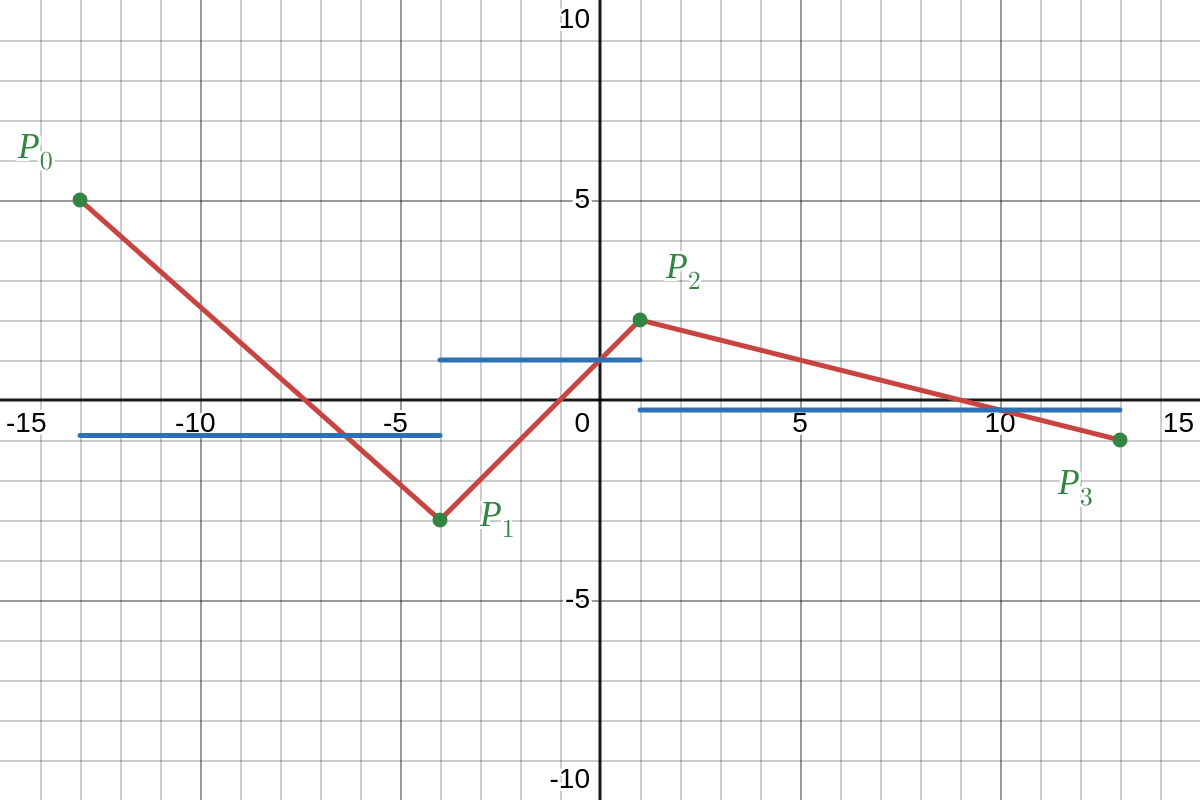
\includegraphics[scale=0.3]{../figures/multipoly_1.png}
\end{center}
\end{minipage}

\par\medskip

da dove si nota chiaramente che con questo approccio la continuità non è assicurata nemmeno al primo grado.

\subsubsection{$\mathbf{s = 2}$: spline quadratiche}
Una soluzione più "liscia" si può avere sfruttando le cosiddette \textbf{spline quadratiche}:
\begin{definition}{Spline quadratica}
	Dati $k + 1$ punti $(x_j, y_j)$ in un intervallo $[a, b]$ con $j = 0, ..., k$ si definisce spline quadratica ($s = 2$) relativa ai $k + 1$ punti la funzione definita a tratti $S_2(x)$ che rispetta le condizioni:
	\begin{enumerate}
		\item $S_2(x)$ è un polinomio di grado 2 se ristretto ad un intervallo $[x_{i - 1}, x_i]$;
		\item $S_2(x_i) = y_i$ per ogni punto $i = 0, ..., k$;
		\item $S_2(x) \in C^1([a, b])$.
	\end{enumerate}
\end{definition}
In questi termini, l'interpolazione lineare a tratti vista finora rappresenta una sorta di interpolazione per \textit{"spline lineari"}, mentre nella prossima sezione vedremo le \textit{spline cubiche}.
Vediamo quindi che le condizioni imposte equivalgono a dire:
\[
	\begin{cases}
		p_i(x_i) = y_i, \quad i = 1, ..., k \\ 
		p_i(x_{i - 1}) = y_{i - 1}, \quad i = 1, ..., k \\ 
		p_i'(x_i) + p_{i + 1}'(x_i), \quad i = 1, ..., k - 1 \\ 
	\end{cases}
\]
cioè abbiamo complessivamente $3k - 1$ condizioni.
Di contro, guardando alla prima condizione si ha che ogni tratto dell'interpolazione avrà forma:
$$
q_i(x) = a_i x^2 + b_i x + c_i, \quad i = 1, ..., k
$$
cioè $3k$ parametri complessivi.

Visto che $3k$ parametri per $3k - 1$ condizioni sono troppi, dobbiamo introdurre un'altra condizione: diciamo che la derivata in $x_0$ deve essere uguale ad un valore fisso $d_0$.

A questo punto basterà trovare $a_i$, $b_i$ e $c_i$ in funzione di $x_{i - 1}$, $x_i$ e la derivata in $x_{i - 1}$ (che chiamiamo $d_{i-1}$), che saranno:
\[
	\begin{cases}
		a_i  =\frac{y_{i}-y_{i-1}}{\left(x_{i-1}-x_{i}\right)^{2}}+\frac{d_{i-1}}{x_{i-1}-x_{i}} \\ 
		b_i = d_{i - 1} -2a_ix_{i-1} \\
		c_i = y_{i}-a_ix_{i}^{2}-b_ix_{i}
	\end{cases}
\]

Calcolando tali valori per ognuno dei $k$ tratti dell'interpolazione si trovano i parametri di ogni quadratica interpolante.


Facendo ciò sull'esempio di prima, preso $d_0 = -2$ e tracciando il grafico, si ha (assieme alla derivata prima e seconda):
\begin{center}
	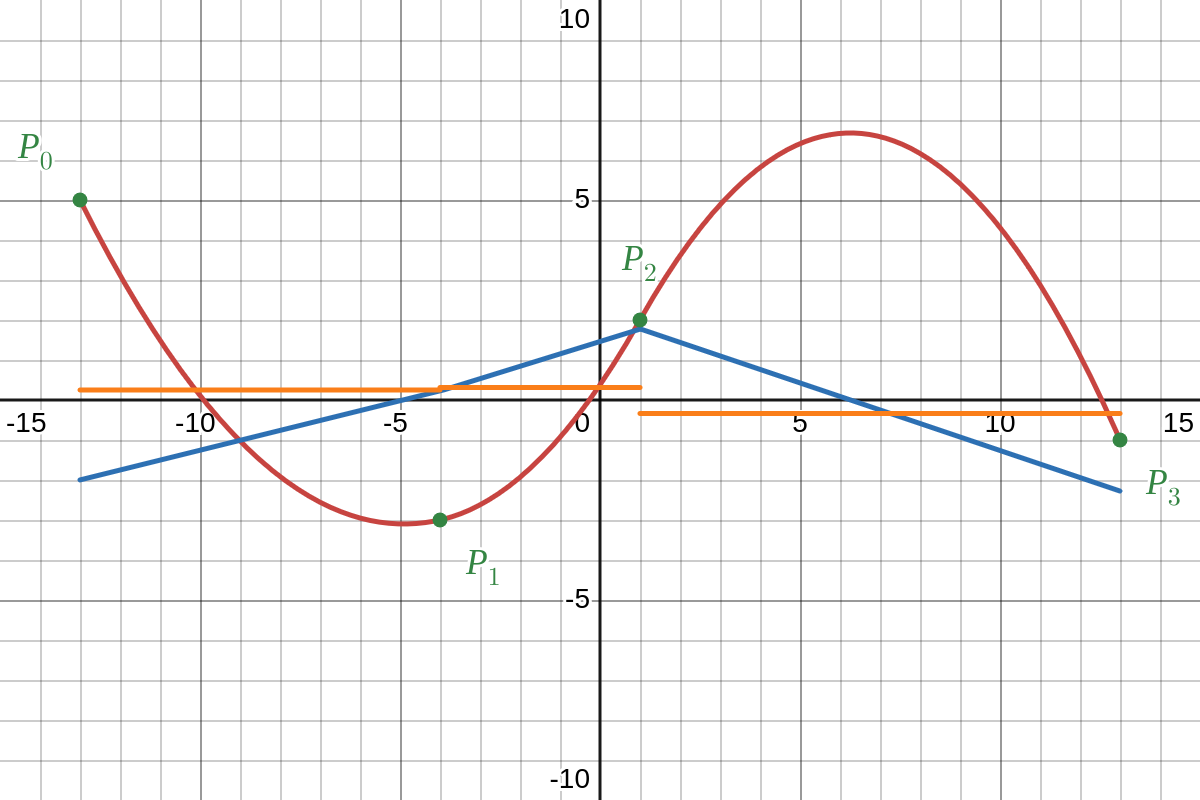
\includegraphics[scale=0.3]{../figures/multipoly_2.png}
\end{center}
da dove notiamo quindi di aver guadagnato la continuità al primo grado, ma ancora non al secondo.
In verità le spline quadratiche non sono molto utili per via delle limitazioni che ci impongono, e vengono usate di rado in contesti reali.
Passiamo quindi a polinomi di grado più alto, molto più di largo uso, cioè $s = 3$.

\subsubsection{$\mathbf{s = 3}$: spline cubica}
Una soluzione ancora più "liscia" si può quindi avere sfruttando le cosiddette \textbf{spline cubiche}.
Queste sono il tipo più comune di spline, e vengono usate in svariati contesti, fra cui ad esempio per tracciare linee "smussate" in computer grafica.

Definiamo quindi:
\begin{definition}{Spline cubica}
	Dati $k + 1$ punti $(x_j, y_j)$ in un intervallo $[a, b]$ con $j = 0, ..., k$ si definisce spline cubica ($s = 3$) relativa ai $k + 1$ punti la funzione definita a tratti $S_3(x)$ che rispetta le condizioni:
	\begin{enumerate}
		\item $S_3(x)$ è un polinomio di grado 3 se ristretto ad un intervallo $[x_{i - 1}, x_i]$;
		\item $S_3(x_i) = y_i$ per ogni punto $i = 0, ..., k$;
		\item $S_3(x) \in C^2([a, b])$.
	\end{enumerate}
\end{definition}
Vediamo quindi che le condizioni imposte equivalgono a dire:
\[
	\begin{cases}
		p_i(x_i) = y_i, \quad i = 1, ..., k \\ 
		p_i(x_{i - 1}) = y_{i - 1}, \quad i = 1, ..., k \\ 
		p_i'(x_i) + p_{i + 1}'(x_i), \quad i = 1, ..., k - 1 \\ 
		p_i''(x_i) + p_{i + 1}''(x_i), \quad i = 1, ..., k - 1 \\ 
	\end{cases}
\]
con una riga in più di condizioni rispetto al caso quadratico dato dal salto da continuità $C^1$ a $C^2$, cioè abbiamo complessivamente $4k - 2$ condizioni.
Di contro, guardando alla prima condizione si ha che ogni tratto dell'interpolazione avrà forma:
$$
c_i(x) = a_i x^3 + b_i x^2 + c_i x + d_i, \quad i = 1, ..., k
$$
cioè $4k$ parametri complessivi.

Come nel caso quadratico, visto che $4k$ parametri per $4k - 2$ condizioni sono troppi, dovremo introdurre 2 nuove condizioni, che modificheranno il tipo di problema che andremo a risolvere:
\begin{itemize}
	\item \textbf{Spline naturale:} si considera questo tipo di spline quando non si ha alcun tipo di informazione oltre i punti da interpolare. In questo caso si assume quindi:
		$$
		p_1''(x_0) = p_k''(x_k) = 0
		$$
		cioè derivata seconda nulla agli estremi di interpolazione $x_0 = a$ e $x_k = b$ di $[a, b]$;
	\item \textbf{Spline periodica:} quando si ritiene che la funzione da approssimare sia periodica, si possono adottare le condizioni:
		$$
		p_1''(x_0) = p_k''(x_k), \quad p_1'(x_0) = p_k'(x_k)
		$$
	\item \textbf{Spline vincolata:} infine, se si conoscono le derivate prime negli estremi di interpolazione $x_0 = a$ e $x_k = b$ si possono imporre le condizioni:
		$$
		p_1'(x_0) = f'(x_0), \quad p_k'(x_k) = f'(x_k)
		$$

		Un altro tipo di spline vincolata potrebbe essere quello da usare nel caso in cui si conoscono derivata prima e seconda nel primo estremo di interpolazione $x_0 = a$.
		In questo caso si impongono le condizioni:
		$$
		p_1'(x_0) = f'(x_0) \quad p_1''(x_0) = f''(x_0)
		$$
		Questo equivale al caso che abbiamo considerato per la spline quadratica (chiamando $f'(x_0) = d_0$ e $f''(x_0) = s_0$), salvo aver dovuto introdurre un ulteriore grado di derivazione.
\end{itemize}

In ogni caso, per punti equispaziati i può dimostrare il seguente teorema:
\begin{theorem}{Esistenza di spline cubiche}
	Presi $x_0, ..., x_k$ nodi equispaziati su un intervallo $[a, b]$, cioè:
	$$
	x_i = a + ih, \quad h = \frac{b - a}{k}, \quad i = 0, ..., k
	$$
	e le valutazioni $y_0, ..., y_k$ di una certa funzione $f(x)$ nei nodi $x_i$, esiste unica la spline naturale $S_3(x)$ passante per i punti $(x_i, y_i)$, $i = 0, ..., k$.
\end{theorem}

Vediamo quindi due procedimenti di calcolo per due dei casi appena definiti, cioè il primo (spline naturale) e l'ultimo (spline vincolata in $x_0$).
Le formule per il calcolo degli altri due casi saranno in qualche modo ricavate in modo equivalente a quelle del primo caso.
\begin{itemize}
	\item Un primo approccio può essere quello di risolvere ognuno dei $k$ sottoproblemi di interpolazione fra $x_{i - 1}$ e $x_i$ applicando l'interpolazione di Hermite, e portandosi dietro le derivate prime $m_i$ (che ancora non conosciamo), interpretate come $f'(x_i)$.
		Si determinano quindi gli $m_i$ imponendo le condizioni sulla derivata seconda agli estremi (abbiamo detto la \textit{condizione naturale}).

		Presi quindi punti equispaziati come sopra, cioè:
		$$
		x_i = a + ih, \quad h = \frac{b - a}{k}, \quad i = 0, ..., k
		$$
		questo procedimento porta alla formazione di spline del tipo:
		$$
		p_i(x) = \left[ f(x_{i - 1}) + \left( m_{i - 1} + \frac{2 f(x_{i - 1})}{h} \right) (x - x_{i - 1})  \right] \left( \frac{x - x_i}{h} \right)^2
		$$
		$$
		+ \left[ f(x_{i}) + \left( m_{i} - \frac{2 f(x_{i })}{h} \right) (x - x_{i})  \right] \left( \frac{x - x_{i - 1}}{h} \right)^2
		$$
		direttamente dall'interpolazione di Hermite, con gli $m_i$ soluzioni del seguente sistema lineare:
		$$
		\begin{pmatrix}
			2 & 1 & 0 & ... & 0 \\ 
			1 & 4 & 1 & ... & 0 \\
			0 & \ddots & \ddots & \ddots & 0 \\
			0 & ... & 1 & 4 & 1 \\
			0 & ... & 0 & 1 & 2
		\end{pmatrix}
		\begin{pmatrix}
			m_0 \\ m_1 \\ m_2 \\ \vdots \\ m_k
		\end{pmatrix}
		=
		\frac{3}{h}
		\begin{pmatrix}
			f(x_1) - f(x_0) \\
			f(x_2) - f(x_0) \\
			f(x_3) - f(x_1) \\
			\vdots \\
			f(x_{k-1}) - f(x_{k-2}) \\
			f(x_k) - f(x_{k-1})
		\end{pmatrix}
		$$
		da dove si nota la matrice $A$ a \textit{˝striscia"}, data dall'interdipendenza fra i tratti della spline.

		Per la dimostrazione seguiremo i passaggi in quest'ordine:
		\begin{enumerate}
			\item Prima troviamo una forma per il polinomio interpolante di Hermite $p_i(x)$ nei nodi $x_{i - 1}$ e $x_{i}$, noti i valori $y_{i - 1}$, $y_i$ e le derivate prime $m_{i - 1}$, $m_i$;
			\item Poi calcoliamo la forma delle derivate seconde del polinomio interpolante agli estremi, in modo da preparare il prossimo passaggio;
			\item Imponiamo le condizioni della spline cubica naturale, cioè derivate seconde agli estremi nulle e continuità $C^2$ nei punti intermedi.
		\end{enumerate}

		Procediamo quindi con la dimostrazione.

		\begin{enumerate}
			\item 
				Vorremo interpolare ogni tratto $x_{i - 1}$, $x_i$ con un polinomio $p_i(x)$ di terzo grado che rispetti:
				\[
					\begin{cases}
						p_i(x_{i - 1}) = f(x_{i - 1}) \\
						p_i(x_i) = f(x_i) \\
						p_i(x_{i - 1}) = m_{i - 1} \\
						p_i(x_i) = m_1
					\end{cases}
				\]
				dove i $k + 1$ valori $m_0, m_1, ..., m_k$ sono le derivate prime che ancora non conosciamo.
				Avremo quindi da Hermite che vorremmo prendere le basi di Lagrange, che posto $x_i - x_{i - 1} = h$ (come si ha da nodi equispaziati) sono:
				$$
				e_{i-1}(x) = \frac{x - x_i}{x_{i-1} - x_i} = -\frac{x - x_i}{h}, \quad e_i(x) = \frac{x - x_{i-1}}{x_i - x_{i-1}} = \frac{x - x_{i - 1}}{h}
				$$
				di cui calcoliamo subito le derivate, in quanto ci serviranno in seguito:
				$$
				e_{i-1}'(x) = -\frac{1}{h}, \quad e_{i}'(x) = \frac{1}{h}, \quad e_{i - 1}''(x) = e_{i}''(x) = 0
				$$

				Avremo quindi le basi di Hermite:
				$$
				h_{0,i-1}\left(x\right) = (1 - 2e_{i - 1}'(x_{i - 1})(x - x_{i-1}))e_{i-1}^2(x) 
				= \left(1+2\frac{x - x_{i-1}}{h}\right)\left(\frac{x-x_{i}}{h}\right)^{2}
				$$
				$$
				h_{0,i}\left(x\right) = (1 - 2e_{i}'(x_i)(x - x_i))e_i^2(x) 
				= \left(1-2\frac{x - x_i}{h}\right)\left(\frac{x-x_{i-1}}{h}\right)^{2}
				$$
				$$
				h_{1,i-1}\left(x\right) = (x - x_{i - 1})e_{i-1}^2(x) = \left(x-x_{i-1}\right)\left(\frac{x-x_{i}}{h}\right)^{2}
				$$
				$$
				h_{1,i}\left(x\right) = (x - x_{i})e_{i}^2(x) = \left(x-x_{i}\right)\left(\frac{x-x_{i-1}}{h}\right)^{2}
				$$
				da cui il polinomio interpolante finale, raccogliendo le basi quadrate comuni e qualche altro termine, è:
				$$
				p_i\left(x\right)=h_{0,i-1}\left(x\right)y_{i-1}+h_{0,i}\left(x\right)y_{i}+h_{1,i-1}\left(x\right)m_{i-1}+h_{1,i}\left(x\right)m_{i}
				$$
				$$
				= \left(1+2\frac{x - x_{i-1}}{h}\right)\left(\frac{x-x_{i}}{h}\right)^{2} y_{i - 1}
				+ \left(1-2\frac{x - x_i}{h}\right)\left(\frac{x-x_{i-1}}{h}\right)^{2} y_i
				$$
				$$
				+ \left(x-x_{i-1}\right)\left(\frac{x-x_{i}}{h}\right)^{2} m_{i - 1}
				+ \left(x-x_{i}\right)\left(\frac{x-x_{i-1}}{h}\right)^{2} m_i
				$$
				$$
				=\left(y_{i-1}+\left(m_{i-1}+\frac{2y_{i-1}}{x_{i}-x_{i-1}}\right)\left(x-x_{i-1}\right)\right)\left(\frac{x-x_{i}}{x_{i}-x_{i-1}}\right)^{2}
				$$
				$$
				+\left(y_{i}+\left(m_{i}-\frac{2y_{i}}{x_{i}-x_{i-1}}\right)\left(x-x_{i}\right)\right)\left(\frac{x-x_{i-1}}{x_{i}-x_{i-1}}\right)^{2}
				$$
				che posto $y_i = f(x_i)$ è esattamente quanto dato prima:
				$$
				p_i(x) = \left[ f(x_{i - 1}) + \left( m_{i - 1} + \frac{2 f(x_{i - 1})}{h} \right) (x - x_{i - 1})  \right] \left( \frac{x - x_i}{h} \right)^2
				$$
				$$
				+ \left[ f(x_{i}) + \left( m_{i} - \frac{2 f(x_{i })}{h} \right) (x - x_{i})  \right] \left( \frac{x - x_{i - 1}}{h} \right)^2
				$$

			\item
				A questo punto resta da ricavare il sistema lineare, che è ciò che ci darà i valori degli $m_i$.
				Per fare ciò calcoliamo la derivata seconda del polinomio interpolante, partendo dal calcolare le derivate secondo delle singole basi di Hermite:
				$$
				h_{0,i-1}''(x) = \frac{2}{h^{3}}\left(h+6x-2x_{i - 1}-4x_{i}\right)
				$$
				$$
				h_{0,i}''(x) = \frac{2}{h^{3}}\left(h-6x+2x_{i}+4x_{i - 1}\right)
				$$
				$$
				h_{1,i-1}''(x) = \frac{1}{h^{2}}\left(6x-2x_{i-1}-4x_{i}\right)
				$$
				$$
				h_{1, i}''(x) = \frac{1}{h^{2}}\left(6x-2x_{i}-4x_{i-1}\right)
				$$
				da cui:
				$$
				p_i''(x) = \frac{2}{h^{3}}\left(h+6x-2x_{i-1}-4x_{i}\right)y_{i-1}+\frac{2}{h^{3}}\left(h-6x+2x_{i}+4x_{i-1}\right)y_{i}
				$$
				$$
				+\frac{1}{h^{2}}\left(6x-2x_{i-1}-4x_{i}\right)m_{i-1}+\frac{1}{h^{2}}\left(6x-2x_{i}-4x_{i-1}\right)m_{i}
				$$

				Ottenuta la derivata seconda del polinomio interpolante, calcoliamola nei punti $x_{i - 1}$ e $x_i$.
				Per $x_{i - 1}$, ad esempio, si avrà:
				$$
				p_i''(x_{i-1}) = \frac{2}{h^{3}}\left(h+6x_{i-1}-2x_{i-1}-4x_{i}\right)y_{i-1}+\frac{2}{h^{3}}\left(h-6x_{i-1}+2x_{i}+4x_{i-1}\right)y_{i}
				$$
				$$
				+\frac{1}{h^{2}}\left(6x_{i-1}-2x_{i-1}-4x_{i}\right)m_{i-1}+\frac{1}{h^{2}}\left(6x_{i-1}-2x_{i}-4x_{i-1}\right)m_{i}
				$$
				$$
				= \frac{2}{h^3} \left( h + 4x_{i-1} - 4x_i \right) y_{i-1} + \frac{2}{h^3} \left(  h - 2x_{i - 1} + 2 x_i \right) y_i
				$$
				$$
				+ \frac{1}{h^2} \left( 4 x_{i - 1} - 4x_i \right) m_{i - 1} + \frac{1}{h^2} \left( 2x_{i - 1} - 2x_i \right) m_i
				$$
				$$
				=  \frac{2}{h^3} (h - 4h) y_{i - 1} + \frac{2}{h^3} (h + 2h) y_i + \frac{1}{h^2} (-4h) m_{i - 1} + \frac{1}{h^2} (-2h) m_i
				$$
				$$
				= -\frac{6}{h^2} y_{i-1} + \frac{6}{h^2} y_i - \frac{4}{h} m_{i - 1} - \frac{2}{h} m_i = \frac{6\left(y_{i}-y_{i-1}\right)}{h^{2}}-\frac{4m_{i-1}+2m_{i}}{h}
				$$
				e con passaggi simili si calcola in $x_i$, per cui:
				$$
				p_i''(x_{i - 1}) = \frac{6\left(y_{i}-y_{i-1}\right)}{h^{2}}-\frac{4m_{i-1}+2m_{i}}{h}
				$$
				$$
				p_i''(x_i) = \frac{2m_{i-1}+4m_{i}}{h}-\frac{6\left(y_{i}-y_{i-1}\right)}{h^{2}}
				$$

			\item
				Avremo a questo punto da applicare le condizioni della spline cubica naturale, cioè derivata seconda nulla agli estremi:
				\[
					\begin{cases}	
						p_1''(x_0) = 0 \implies 2m_0 + m_1 = \frac{3}{h} \left( f(x_1) - f(x_0) \right) \\
						p_k''(x_k) = 0 \implies 2m_k + m_{k - 1} = \frac{3}{h} \left( f(x_k) - f(x_{k - 1}) \right) \\
					\end{cases}
				\]
				e derivate seconde continue nei punti intermedi:
				$$
				p_i''(x_i) = p_{i+1}''(x_{i}) \implies m_{i - 1} + 4 m_i + m_{i + 1} = \frac{3}{h} f(x_{i + 1}) - f(x_{i - 1})
				$$
				da cui il sistema lineare che corredava la forma del polinomio di Hermite, e quindi la tesi. \qed
		\end{enumerate}

	\item Se si vuole imporre il vincolo "a sinistra" della derivata prima e seconda, si può procedere in maniera analoga a quanto fatto nel caso quadratico, cioe prendere i tratti polinomiali:
		$$
		c_i(x) = a_i x^3 + b_i x^2 + c_i x + d_i, \quad i = 1, ..., k
		$$
		e trovare gli $a_i$, $b_i$, $c_i$ e $d_i$ in funzione di $x_{i - 1}$, $x_i$ e le due derivate consecutive in $x_{i - 1}$ (che chiamiamo $d_{i - 1}$ e $s_{i- 1}$, rispettivamente primo e secondo grado).

		Visto che trovare direttamente i quattro problemi può essere difficile, decidiamo invece di trovare le 4 basi ortogonali $b_1$, $b_2$, $b_3$ e $b_4$ (di cui le prime 3 equivalenti a quelle di Hermite, e l'ultima corrispondente alla condizione derivata seconda in $x_{i - 1}$), che rispettano quindi le condizioni:
		$$
		b_1 : 
		\begin{cases}
			b_1(x_{i - 1}) = 1 \\
			b_1(x_i) = 0 \\
			b_1'(x_{i - 1}) = 0 \\
			b_1''(x_{i - 1}) = 0 \\
		\end{cases}, \quad
		b_2 : 
		\begin{cases}
			b_2(x_{i - 1}) = 0 \\
			b_2(x_i) = 1 \\
			b_2'(x_{i - 1}) = 0 \\
			b_2''(x_{i - 1}) = 0 \\
		\end{cases}
		$$

		$$
		b_3 : 
		\begin{cases}
			b_3(x_{i - 1}) = 0 \\
			b_3(x_i) = 0 \\
			b_3'(x_{i - 1}) = 1 \\
			b_3''(x_{i - 1}) = 0 \\
		\end{cases}, \quad
		b_4 : 
		\begin{cases}
			b_3(x_{i - 1}) = 0 \\
			b_3(x_i) = 0 \\
			b_3'(x_{i - 1}) = 0 \\
			b_3''(x_{i - 1}) = 1 \\
		\end{cases}
		$$

		Queste si potranno ricavare, direttamente dall'imposizione delle condizioni, come:
		\begin{enumerate}
			\item $b_{1}\left(x,x_{i-1},x_{i}\right)=a_{b1}\left(x_{i-1},x_{i}\right)x^{3}+b_{b1}\left(x_{i-1},x_{i}\right)x^{2}+c_{b1}\left(x_{i-1},x_{i}\right)x+d_{b1}\left(x_{i-1},x_{i}\right)$,
				con:
				\begin{itemize}
					\item $a_{b1}\left(x_{i-1},x_{i}\right)=\frac{1}{\left(x_{i-1}-x_{i}\right)^{3}}$;
					\item $b_{b1}\left(x_{i-1},x_{i}\right)=-3a_{b1}\left(x_{i-1},x_{i}\right)x_{i-1}$;
					\item $c_{b1}\left(x_{i-1},x_{i}\right)=3a_{b1}\left(x_{i-1},x_{i}\right)x_{i-1}^{2}$;
					\item $d_{b1}\left(x_{i-1},x_{i}\right)=1-a_{b1}\left(x_{i-1},x_{i}\right)x_{i-1}^{3}$.
				\end{itemize}
			\item Questa è banalmente $b_{2} \left( x, x_{i-1}, x_{i} \right) = 1 - b_{1}\left(x,x_{i-1},x_{i}\right)$;
			\item $b\left(x,x_{i-1},x_{i}\right)=a_{b3}\left(x_{i-1},x_{i}\right)x^{3}+b_{b3}\left(x_{i-1},x_{i}\right)x^{2}+c_{b3}\left(x_{i-1},x_{i}\right)x+d_{b3}\left(x_{i-1},x_{i}\right)$,
				con:
				\begin{itemize}
					\item $a_{b3}\left(x_{i-1},x_{i}\right)=\frac{x_{i-1}-x_{i}}{\left(x_{i}-x_{i-1}\right)^{3}}$;
					\item $b_{b3}\left(x_{i-1},x_{i}\right)=-3a_{b3}\left(x_{i-1},x_{i}\right)x_{i-1}$;
					\item $c_{b3}\left(x_{i-1},x_{i}\right)=1+3a_{b3}\left(x_{i-1},x_{i}\right)x_{i-1}^{2}$;
					\item $d_{b3}\left(x_{i-1},x_{i}\right)=-a_{b3}\left(x_{i-1},x_{i}\right)x_{i-1}^{3}-x_{i-1}$.
				\end{itemize}
			\item $b\left(x,x_{i-1},x_{i}\right)=a_{b4}\left(x_{i-1},x_{i}\right)x^{3}+b_{b4}\left(x_{i-1},x_{i}\right)x^{2}+c_{b4}\left(x_{i-1},x_{i}\right)x+d_{b4}\left(x_{i-1},x_{i}\right)$,
				con:
				\begin{itemize}
					\item $a_{b4}\left(x_{i-1},x_{i}\right)=\frac{\left(x_{i}-x_{i-1}\right)^{2}}{2\left(x_{i-1}-x_{i}\right)^{3}}$;
					\item $b_{b4}\left(x_{i-1},x_{i}\right)=\frac{1}{2}-3a_{b4}\left(x_{i-1},x_{i}\right)x_{i-1}$;
					\item $c_{b4}\left(x_{i-1},x_{i}\right)=3a_{b4}\left(x_{i-1},x_{i}\right)x_{i-1}^{2}-x_{i-1}$;
					\item $d_{b4}\left(x_{i-1},x_{i}\right)=\frac{1}{2}x_{i-1}^{2}-a_{b4}\left(x_{i-1},x_{i}\right)x_{i-1}^{3}$.
				\end{itemize}
		\end{enumerate}

		A questo punto basterà definire ogni tratto polinomiale $c_i$ come:
		$$
		c_{i}\left(x\right)=b\left(x,x_{i-1},x_{i}\right)y_{i-1}+b\left(x,x_{i-1},x_{i}\right)y_{i}+b\left(x,x_{i-1},x_{i}\right)d_{i-1}+b\left(x,x_{i-1},x_{i}\right)s_{i-1}\
		$$
		dove gli $d_{i-1}$ e $s_{i-1}$ sono rispettivamente la derivata prima e seconda in ogni punto, data per il punto $x_0$ e ricavata dal tratto precedente per ogni tratto successivo.

		Un interpolazione di questo tipo per l'esempio considerato nelle scorse sezioni ha l'aspetto, prese $d_{0} = 1$ e $s_{0} = -1$ e tracciate derivata prima e seconda:
		\begin{center}
			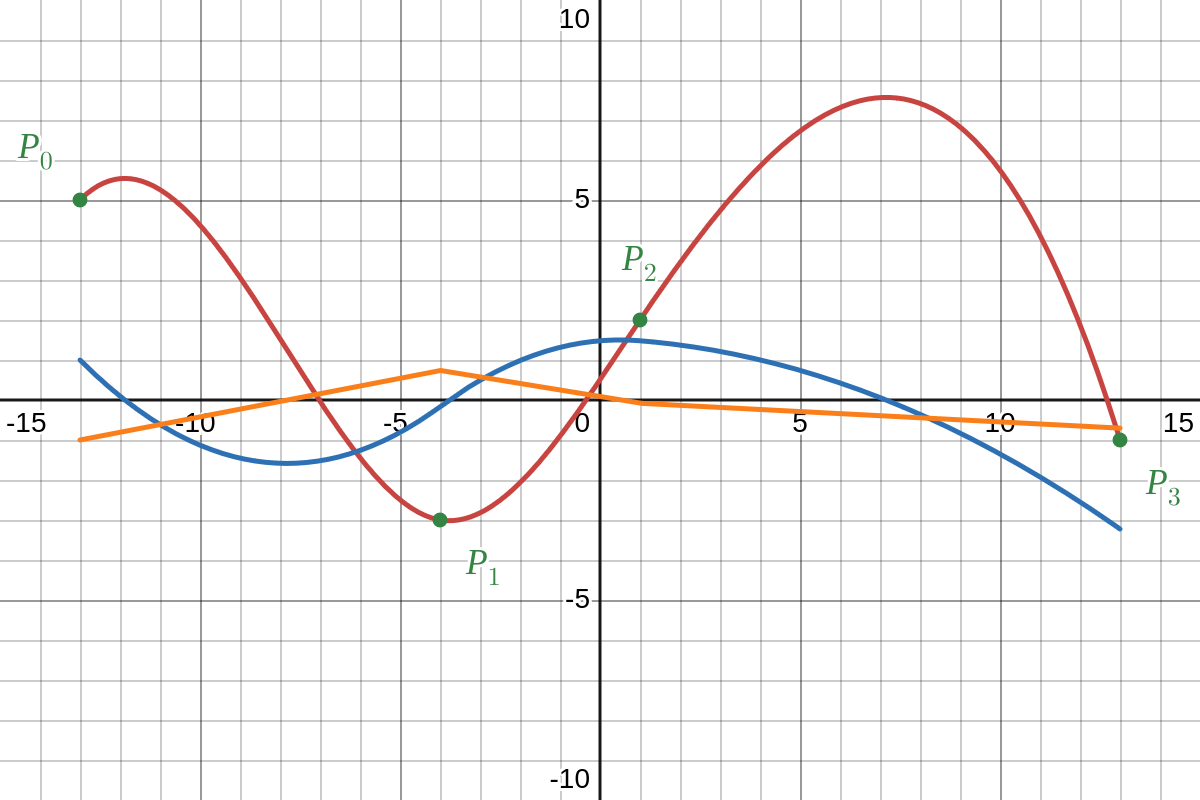
\includegraphics[scale=0.3]{../figures/multipoly_3.png}
		\end{center}
		da dove notiamo che la derivata fino al secondo grado resta continua, da cui la condizione 3 è rispettata.

		Vediamo che in verità si può risolvere in qualche modo anche lo scorso tipo di problema con questo metodo, semplicemente imponendo $s_0 = 0$ e cercando $d_0$ perché risulti $s_k = 0$.

		\par\medskip
		\noindent

		\begin{minipage}{\textwidth}
		Nell'esempio, questo si ottiene per $d_0 \approx -1.574$, con relativo grafico:
		\begin{center}
			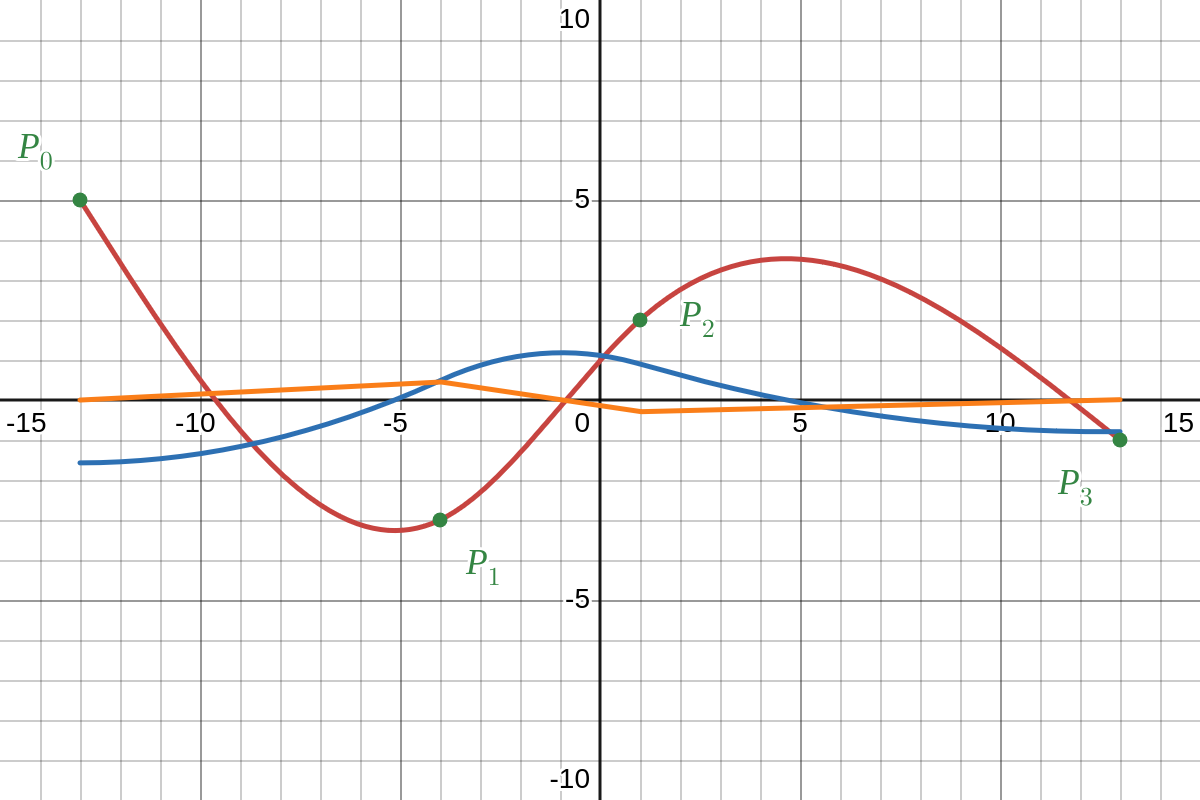
\includegraphics[scale=0.3]{../figures/multipoly_nat.png}
		\end{center}
		\end{minipage}
\end{itemize}

Esempi di questi tipi di interpolazione si possono trovare sempre su Desmos, al link \url{https://www.desmos.com/calculator/gm1idqauiy} (da qui sono state generate le figure).

\subsection{Approssimazione ai minimi quadrati}
Un altro approccio per l'approssimazione di insiemi di punti, specialmente nel caso questi siano imponenti in dimensioni, può essere dato dall'\textbf{approssimazione ai minimi quadrati}.

Un caso banale di questo tipo di approssimazione può essere quello della \textit{regressione lineare}: dato un insieme di $k + 1$ punti $(x_j, y_j)$, si cerca la retta che minimizza la distanza quadratica da ogni punto.
In qusto caso la retta prende il nome di \textbf{funzione modello}.

Generalizziamo quindi questo approssimazione in 2 direzioni:
\begin{itemize}
	\item Ammettiamo che si abbiano più punti che funzioni modello (che possiamo intendere come le basi polinomiali usate finora);
	\item Amettiamo l'utilizzo di funzioni modello non polinomiali.
\end{itemize}

Formalmente, quindi, dati $k + 1$ punti $(x_0, y_0), ..., (x_k, y_k)$ punti con $y_j = f(x_j)$ e $m + 1$ funzioni modello $G_0(x), ..., G_m(x)$ con $m \leq x$ cercheremo l'approssimante $\Phi(x) \approx f(x)$ della forma:
$$
\Phi(x) = \sum_{i = 0}^m G_i(x) \cdot c_i, \quad c_i \in \mathbb{R}
$$
con $c_i$ da trovare, cioè la combinazione lineare ottima (definiremo cosa significa ottima fra poco) delle funzioni modello.

\begin{itemize}
	\item 
		Ad esempio, la regressione lineare quella data dalle funzioni modello:
		$$
		G_0(x) = 1, \quad G_1(x) = x
		$$
		approssimante $k + 1 = \#$ punti nel grafico;
	\item Potremmo avere altri tipi di funzioni modello.
		Ad esempio potremmo avere:
		$$
		G_0(x) = e^{2x}, \quad G_1(x) = \sin\left( \frac{x}{2} \right), \quad G_2(x) = \frac{1}{3x^2 + 4}
		$$
		In questo caso l'approssimante avrebbe una forma del tipo:
		$$
		\Phi(x) = c_0 e^{2x} + c_1 \sin \left( \frac{x}{2} \right) + \frac{c_2}{3x^2 + 4}
		$$
\end{itemize}

\par\smallskip

A questo punto il problema è capire cosa significa dire che $\Phi(x)$ passa \textit{"vicino"} ai punti $(x_j, y_j)$, cioè qual'è la funzione da ottimizzare per trovare i $c_i$ ottimi in modo che risulti $\Phi(x) \approx f(x)$.
Dobbiamo quindi definire una qualche funzione di errore $\psi(c_0, ..., c_m) : \mathbb{R}^{m + 1} \rightarrow \mathbb{R}^+$.

Vediamo come definire tale funzione.
\begin{itemize}
	\item Un primo approccio potrebbe essere il semplice \textit{scarto}:
		$$
		\psi(c_0, ..., c_m) = \sum_{i = 0}^k \left( \Phi(x_i) - y_i \right)
		$$
		Questa ha il problema di poter dare cancellazione, cioè errori di punti diversi potrebbero annullarsi, per dare valori di $\psi$ bassi quando in realtà la funzione è molto lontana da $f(x)$;
	\item Un approccio migliore è quindi quello di prendere lo \textit{scarto assoluto}:
		$$
		\psi(c_0, ..., c_m) = \sum_{i = 0}^k \Big| \Phi(x_i) - y_i \Big|
		$$
		In questo caso non soffriremo di cancellazione, ma avremo il problema che $\psi$ non è differenziabile (si avranno punti angolosi dati dal valore assoluto);
	\item L'approccio migliore risulta quindi:
		$$
		\psi(c_0, ..., c_m) = \sum_{i = 0}^k \left( \Phi(x_i) - y_i \right)^2
		$$
		cioè lo \textit{scarto quadratico}, che risolve sia i problemi della cancellazione che della continuità $C^1$.
\end{itemize}

Il metodo dei minimi quadrati consisterà quindi nello scegliere:
$$
c = 
\begin{pmatrix}
	c_0 \\ c_1 \\ \vdots \\ c_m
\end{pmatrix}
\in \mathbb{R}^{m + 1}
$$
tale che:
$$
c = \min_{c \in \mathbb{R}^{m + 1}} \psi(c)
$$
cioè $c$ è punto di minimo di $\psi(c)$.

Dovremo quindi minimizzare:
$$
\psi(c) = \sum_{i = 0}^k \left( \Phi(x_i) - y_i \right)^2 = \sum_{i = 0}^k \left( \sum_{j = 0}^m c_j \cdot G_j(x_i) - y_i \right)^2
$$
cioè in forma matriciale, posti:
$$
A =
\begin{pmatrix}
	G_0(x_0) & G_1(x_0) & ... & G_m(x_0) \\
	\vdots & & & \vdots \\
	G_0(x_0) & G_1(x_1) & ... & G_m(x_k)
\end{pmatrix}, \quad
c =
\begin{pmatrix}
	c_0 \\ \vdots \\ c_m
\end{pmatrix}, \quad
b = 
\begin{pmatrix}
	y_0 \\ \vdots \\ y_k
\end{pmatrix}
$$
con $A \in \mathbb{R}^{ (k + 1) \times (m + 1) }$, $c \in \mathbb{R}^{m + 1}$, $b \in \mathbb{R}^{k + 1}$, equivale a:
$$
\psi(c) = \sum_{i = 0}^k \left( (Ac)_i - b_i \right)^2 = \Big| Ac - b \Big|_2^2
$$

Stiamo quindi minimizzando la norma quadratica del residuo di $Ac = b$, che dalle dimensioni della matrice $A$ e i vettori $c$ e $b$ è un sistema sovradeterminato (più equazioni che incognite):
$$
c^* = \min_{c \in \mathbb{R}^{m + 1}} |Ac - b|_2
$$
Possiamo quindi risolvere interpretando il sistema come uno di quelli visti in 11.1, quindi sfruttando le \textbf{equazioni normali} o la \textbf{decomposizione QR}.

\subsubsection{Implementazione MATLAB di un approssimatore ai quadrati minimi}
Vediamo quindi come implementare questo approccio in MATLAB.

\lstset{language=matlab, style=codestyle}

Abbiamo già a disposizione una funzione, \lstinline|least_squares()|, definita in 12.2.9 per la risoluzione di sistemi sovradeterminati usando la decomposizione QR.
Ci mancherà quindi da scrivere una funzione che calcola il valore della matrice $A$, valutando le funzioni in base $G_i$, e che campiona una certa funzione $f(x)$ in determinati punti $x_i$ per generare un vettore di $y_i$, magari usando la \lstinline|linspace()|, così da avere un insieme di nodi equispaziati del tipo:
$$
x_i = l + ih, \quad i = 0, ..., k - 1
$$
$$
h = \frac{u - l}{k - 1}
$$

Per il problema di come rappresentare le $G_i$ usiamo dei \textit{function handle}, dichiarati come segue:
\begin{lstlisting}[language=matlab, style=codestyle]	
% un function handle alla funzione f(x) = x^2
f = @(x) x.^2
% si usa come: f(2) -> 4
\end{lstlisting}
Una base potrà quindi essere costruita racchiudendo più handle di questo tipo in un \textit{array di celle}.

Prendiamo per adesso la base:
$$
G_0(x) = e^x, \quad G_1(x) = \frac{1}{x}, \quad G_2(x) = \sin(x)
$$

\par\medskip
\noindent

\begin{minipage}{\textwidth}
Avremo allora una funzione del tipo:
\lstinputlisting{../code/matlab/approx_trasc.m}
\end{minipage}

\par\medskip

Attraverso questa funzione potremo calcolare i coefficienti $c$ che minimizzano lo scarto quadratico sugli \lstinline|n| punti fra \lstinline|l| e \lstinline|u|.

\par\smallskip

Prendiamo l'esempio della funzione:
$$
f\left(x\right)=\left(2x-3\right)\left(x-3\right)\left(x-4\right)\left(x-5\right)
$$

Definiremo questa, in MATLAB, come segue:
\begin{lstlisting}[language=matlab, style=codestyle]	
f = @(x) (2.*x - 3).*(x - 3).*(x - 4).*(x - 5);
\end{lstlisting}

Potremo allora trovare i coefficienti $c$ di un approssimazione in forma:
$$
a(x) = c_{0}\cdot e^{x}+c_{1}\cdot\frac{1}{x}+c_{2}\cdot\sin\left(x\right)
$$
usando la funzione MATLAB appena implementata:
\begin{lstlisting}[language=matlab, style=codestyle]	
>> approx_trasc(f, 0.1, 6, 100)

ans =
    0.0596
   21.2591
    1.8092
\end{lstlisting}

\par\medskip
\noindent

\begin{minipage}{\textwidth}
cioè $c_0 = 0.0596$, $c_1 = 21.2591$, $c_2 = 1.8092$, che sul grafico dà:
\begin{center}
	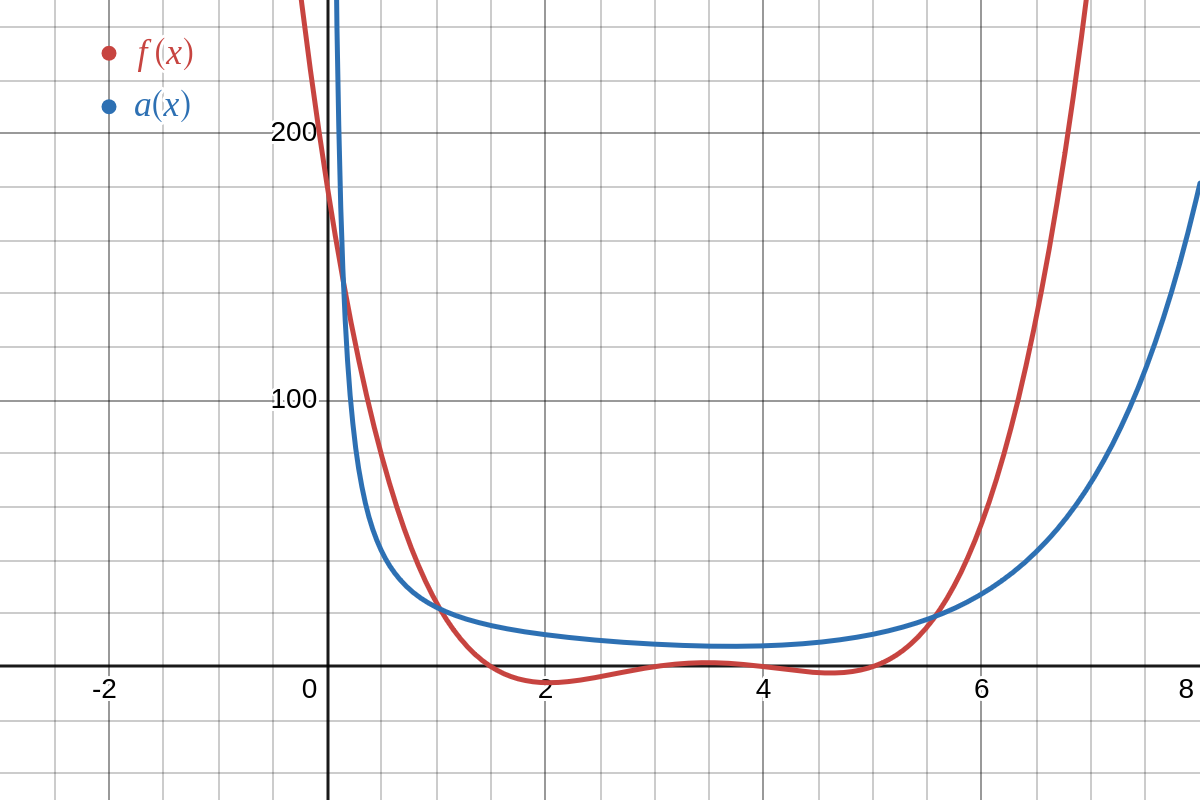
\includegraphics[scale = 0.28]{../figures/trasc_approx.png}
\end{center}
\end{minipage}

\par\medskip

Per un errore medio di:
$$
\varepsilon = \sqrt{\sum_{i = i}^{100} \left( f(x_i) - a(x_i) \right)^2} \approx 163.141
$$

Notiamo quindi che la funzione non passa necessariamente per nessuno dei punti campianati, ma riduce l'errore medio lungo tutta la regione campionata.

Potremmo renderci conto che la maggior parte dell'errore è data dal fatto che cerchiamo di approssimare la funzione nella regione $0.1 \sim 0.7$, che ci porta ad avere un errore più grande nella zona vicino all'asse $x$.
Se fossimo interessati ad ottenere un'approssimazione più accurata in questa regione, potremmo richiamare la funzione aumentando il bound $l$:
\begin{lstlisting}[language=matlab, style=codestyle]	
>> approx_trasc(f, 0.7, 6, 100)

ans =
    0.0825
    7.4361
    5.0514
\end{lstlisting}

\par\medskip
\noindent

\begin{minipage}{\textwidth}
cioè $c_0 = 0.0825$, $c_1 = 7.4361$, $c_2 = 5.0514$, che sul grafico dà:
\begin{center}
	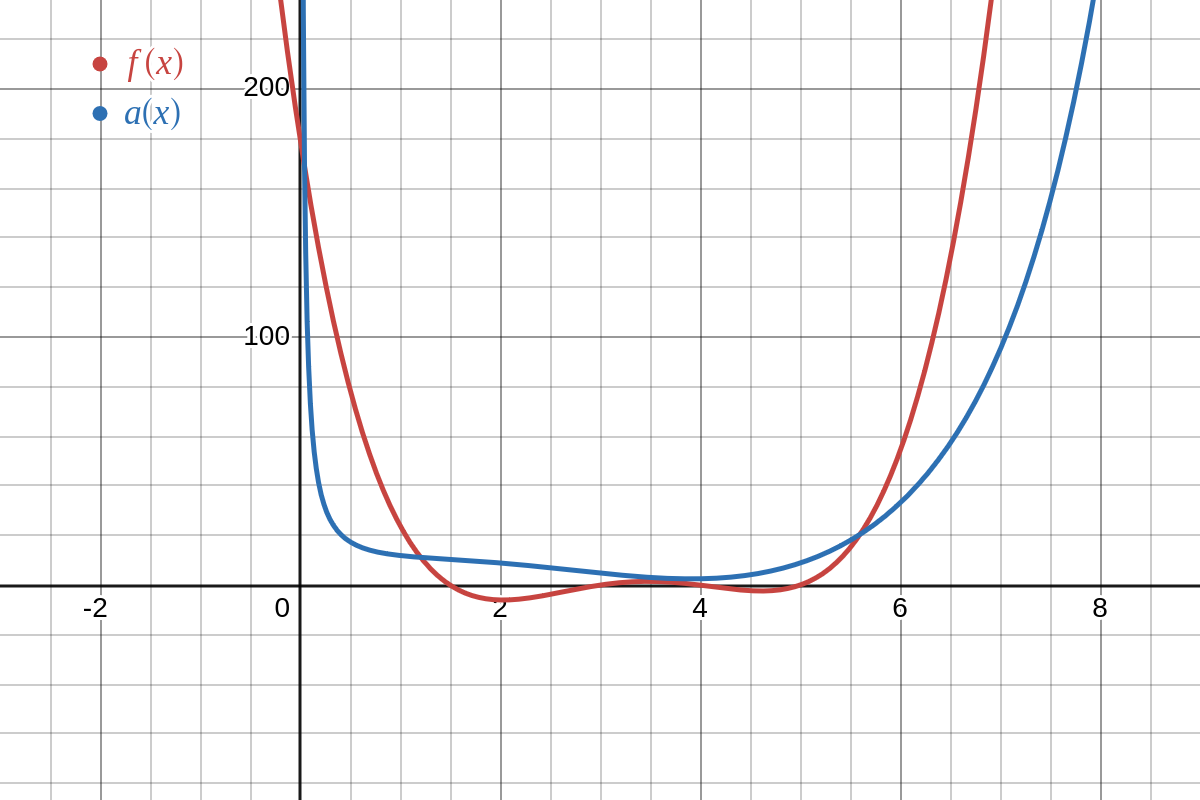
\includegraphics[scale = 0.28]{../figures/trasc_approx_better.png}
\end{center}
\end{minipage}

\par\medskip

Per un errore medio di:
$$
\varepsilon \approx 106.392
$$
sul nuovo intervallo, che è già più accurato.

\end{document}


\documentclass[a4paper,11pt]{article}
\usepackage[a4paper, margin=8em]{geometry}

% usa i pacchetti per la scrittura in italiano
\usepackage[french,italian]{babel}
\usepackage[T1]{fontenc}
\usepackage[utf8]{inputenc}
\frenchspacing 

% usa i pacchetti per la formattazione matematica
\usepackage{amsmath, amssymb, amsthm, amsfonts}

% usa altri pacchetti
\usepackage{gensymb}
\usepackage{hyperref}
\usepackage{standalone}

% imposta il titolo
\title{Appunti Calcolo Numerico}
\author{Luca Seggiani}
\date{2025}

% disegni
\usepackage{pgfplots}
\pgfplotsset{width=10cm,compat=1.9}

% imposta lo stile
% usa helvetica
\usepackage[scaled]{helvet}
% usa palatino
\usepackage{palatino}
% usa un font monospazio guardabile
\usepackage{lmodern}

% tikz in sans
\tikzset{every picture/.style={/utils/exec={\sffamily}}}

\renewcommand{\rmdefault}{ppl}
\renewcommand{\sfdefault}{phv}
\renewcommand{\ttdefault}{lmtt}

% circuiti
\usepackage{circuitikz}
\usetikzlibrary{babel}

% disponi il titolo
\makeatletter
\renewcommand{\maketitle} {
	\begin{center} 
		\begin{minipage}[t]{.8\textwidth}
			\textsf{\huge\bfseries \@title} 
		\end{minipage}%
		\begin{minipage}[t]{.2\textwidth}
			\raggedleft \vspace{-1.65em}
			\textsf{\small \@author} \vfill
			\textsf{\small \@date}
		\end{minipage}
		\par
	\end{center}

	\thispagestyle{empty}
	\pagestyle{fancy}
}
\makeatother

% disponi teoremi
\usepackage{tcolorbox}
\newtcolorbox[auto counter, number within=section]{theorem}[2][]{%
	colback=blue!10, 
	colframe=blue!40!black, 
	sharp corners=northwest,
	fonttitle=\sffamily\bfseries, 
	title=Teorema~\thetcbcounter: #2, 
	#1
}

% disponi definizioni
\newtcolorbox[auto counter, number within=section]{definition}[2][]{%
	colback=red!10,
	colframe=red!40!black,
	sharp corners=northwest,
	fonttitle=\sffamily\bfseries,
	title=Definizione~\thetcbcounter: #2,
	#1
}

% disponi problemi
\newtcolorbox[auto counter, number within=section]{problem}[2][]{%
	colback=green!10,
	colframe=green!40!black,
	sharp corners=northwest,
	fonttitle=\sffamily\bfseries,
	title=Problema~\thetcbcounter: #2,
	#1
}

% disponi codice
\usepackage{listings}
\usepackage[table]{xcolor}

\definecolor{codegreen}{rgb}{0,0.6,0}
\definecolor{codegray}{rgb}{0.5,0.5,0.5}
\definecolor{codepurple}{rgb}{0.58,0,0.82}
\definecolor{backcolour}{rgb}{0.95,0.95,0.92}

\lstdefinestyle{codestyle}{
		backgroundcolor=\color{black!5}, 
		commentstyle=\color{codegreen},
		keywordstyle=\bfseries\color{magenta},
		numberstyle=\sffamily\tiny\color{black!60},
		stringstyle=\color{green!50!black},
		basicstyle=\ttfamily\footnotesize,
		breakatwhitespace=false,         
		breaklines=true,                 
		captionpos=b,                    
		keepspaces=true,                 
		numbers=left,                    
		numbersep=5pt,                  
		showspaces=false,                
		showstringspaces=false,
		showtabs=false,                  
		tabsize=2
}

\lstdefinestyle{shellstyle}{
		backgroundcolor=\color{black!5}, 
		basicstyle=\ttfamily\footnotesize\color{black}, 
		commentstyle=\color{black}, 
		keywordstyle=\color{black},
		numberstyle=\color{black!5},
		stringstyle=\color{black}, 
		showspaces=false,
		showstringspaces=false, 
		showtabs=false, 
		tabsize=2, 
		numbers=none, 
		breaklines=true
}

\lstdefinelanguage{javascript}{
	keywords={typeof, new, true, false, catch, function, return, null, catch, switch, var, if, in, while, do, else, case, break},
	keywordstyle=\color{blue}\bfseries,
	ndkeywords={class, export, boolean, throw, implements, import, this},
	ndkeywordstyle=\color{darkgray}\bfseries,
	identifierstyle=\color{black},
	sensitive=false,
	comment=[l]{//},
	morecomment=[s]{/*}{*/},
	commentstyle=\color{purple}\ttfamily,
	stringstyle=\color{red}\ttfamily,
	morestring=[b]',
	morestring=[b]"
}

% disponi sezioni
\usepackage{titlesec}

\titleformat{\section}
	{\sffamily\Large\bfseries} 
	{\thesection}{1em}{} 
\titleformat{\subsection}
	{\sffamily\large\bfseries}   
	{\thesubsection}{1em}{} 
\titleformat{\subsubsection}
	{\sffamily\normalsize\bfseries} 
	{\thesubsubsection}{1em}{}

% disponi alberi
\usepackage{forest}

\forestset{
	rectstyle/.style={
		for tree={rectangle,draw,font=\large\sffamily}
	},
	roundstyle/.style={
		for tree={circle,draw,font=\large}
	}
}

% disponi algoritmi
\usepackage{algorithm}
\usepackage{algorithmic}
\makeatletter
\renewcommand{\ALG@name}{Algoritmo}
\makeatother

% disponi numeri di pagina
\usepackage{fancyhdr}
\fancyhf{} 
\fancyfoot[L]{\sffamily{\thepage}}

\makeatletter
\fancyhead[L]{\raisebox{1ex}[0pt][0pt]{\sffamily{\@title \ \@date}}} 
\fancyhead[R]{\raisebox{1ex}[0pt][0pt]{\sffamily{\@author}}}
\makeatother

\begin{document}

% sezione (data)
\section{Lezione del 28-04-25}

% stili pagina
\thispagestyle{empty}
\pagestyle{fancy}

% testo
\subsection{Approssimazione di integrali}
Vorremo quindi approssimare funzioni del tipo:
$$
I(\rho \cdot f) = \int_a^b f(x) \cdot \rho(x) \, dx
$$
dove $f: [a, b] \rightarrow \mathbb{R}$ continua $\in C\left([a, b]\right)$, mentre $\rho(x) : [a, b] \rightarrow \mathbb{R}$ sempre continua $\in C\left([a, b]\right)$ è una funzione particolare, spesso la funzione unitaria o comunque una funzione detta \textbf{funzione peso} tale che:
\begin{itemize}
	\item $\rho(x)$ è positiva:
		$$ \rho(x) \geq 0 $$
	\item $\rho(x)$ rispetta le condizioni:
		$$ m_k = \int_a^b x^k \rho(x) \, dx < +\infty, \quad \forall k = 0, 1, ... $$
\end{itemize}

Veniamo alle motivazioni dell'approssimazione di integrali. 
Potremmo voler approssimare integrali del tipo:
$$
\int_a^b f(x) \, dx \quad \left( \rho(x) = 1 \right)
$$
per una serie di motivi:
\begin{itemize}
	\item Di molte funzioni non si può trovare un'espressione semplice della primitiva di $f$ (funzioni ellittiche, funzioni su più variabili, ecc...);
	\item Anche se esiste la primitiva potrebbe essere particolarmente oneroso in termini di risorse computazioniali calcolarla o valutarla in un punto per ottenere l'integrale;
	\item Come nel caso dell'approssimazione e dell'interpolazione, ci sono casi in cui della $f$ si conoscono solo alcuni punti, cioè non se ne ha un'espressione esplicita che possiamo integrare. Vedremo che sarà questo il caso più comune.
\end{itemize}

Prendiamo quindi il caso dove conosciamo una serie di punti $(x_i, f(x_i))$ di $f(x)$.
L'idea per approssimare l'integrale sarà di considerare una formula del tipo:
$$
\int_a^b f(x) \rho(x) \, dx \approx \sum_{i = 0}^n f(x_i) \cdot a_i
$$
con:
$$
a \leq x_0 < x_1 < ... < x_n \leq b
$$
In questo caso chiamiamo gli $x_i$ \textbf{nodi} e gli $a_i$ \textbf{pesi}, e la formula \textbf{formula di quadratura}.
Si ha quindi che una formula di quadratura è univocamente determinata una volta decisi nodi e pesi.

Definiamo quindi formalmente:
\begin{definition}{Formula di quadratura}
	Dati un intervallo $[a, b]$ e $\rho(x)$, definiamo $J_n(\circ)$ formula di quadratura su $(n + 1)$ nodi $x_0, ..., x_n$ con pesi $a_0, ..., a_n$ la funzione:
	\begin{itemize}
		\item Di questa forma:
	$$
	J_n : C\left([a, b]\right) \rightarrow \mathbb{R}
	$$
	tale che:
	$$
	f \rightarrow \sum_{i=0}^n f(x_i) \cdot a_i
	$$
		\item
	O equivalentemente:
	$$
	J_n : \mathbb{R}^{n + 1} \rightarrow \mathbb{R}
	$$
	tale che:
	$$
	\begin{pmatrix}
		f_0 \\ \vdots \\ f_n
	\end{pmatrix} 
	\rightarrow
	\sum_{i=0}^n f_i \cdot a_i
	$$
	\end{itemize}
\end{definition}

Possiamo quindi definire l'errore:
\begin{definition}{Errore della formula di quadratura}
	L'errore della formula di quadratura $J_n(\circ)$ si definisce come:
	$$
	E_n(f) = \int_a^b f(x) \rho(x) \, dx - J_n(f) = \int_a^b f(x) \rho(x) \, dx - \sum_{i = 0}^n f(x_i) \cdot a_i
	$$
	anche questa tale che:
	$$
	E_n : C\left([a, b]\right) \rightarrow \mathbb{R}
	$$
	con:
	$$
	f \rightarrow E_n(f)
	$$
\end{definition}

Ossserviamo che sia $J_n$ che $E_n$ sono funzioni lineari, in quanto date $f_1, f_2 \in C\left([a, b]\right)$ e $c_1, c_2 \in \mathbb{R}$:
$$
J_n (c_1 f_1 + c_2 f_2) = \sum_{i = 0}^n a_i (c_1 f_1 + c_2 f_2)(x_i) 
= \sum_{i = 0}^n a_i ( c_1 f_1(x_i) + c_2 f_2(x_i) )
$$
$$
= \sum_{i = 0}^n \left( a_i c_1 f_1 (x_i) + a_i c_2 f_2 (x_i) \right)
= c_1 \sum_{i = 0}^n a_i f_1 (x_i) + c_2 \sum_{i = 0}^n a_i f_2 (x_i)
= c_1 J_n(f_1) + c_2 J_n(f_2)
$$
e analogamente con $E_n$. \qed

Potremmo quindi chiederci quando una formula di quadratura è accurata.
Potremmo definire un primo indicatore detto \textbf{grado di precisione}.
\begin{definition}{Grado di precisione}
	Data $J_n$ formula di quadratura definiamo grado di precisione (a volte detto \textit{grado di precisione algebrico}) il naturale $m \in \mathbb{N}$ tale che:
	$$
		E_n(1) = E_n(x) = ... = E_n (x^m) = 0
	$$
	presi i monomi $x_0, ..., x^m$, cioè per cui:
	$$
	E_n(x^{m + 1}) \neq 0
	$$
\end{definition}

Osserviamo che per la proprietà di linearità di $E_n$ e $J_n$ appena dimostrata, si ha che $J_n$ ha grado di precisione $m$ se e solo se $J_n$ integra esattamente tutti i polinomi di grado $\leq m$ (che altro non sono che combinazioni lineari dei monomi $x_0, ..., x^{m}$ appena considerati).

\subsubsection{Formula dei trapezi}

Prendiamo ad esempio $\rho = 1$, l'intervallo $[a, b] = [-1, 1]$ con $n = 1$, per cui consideriamo solo gli estremi $x_0 = -1$, $x_1 = 1$.
In questo caso avremo la formula di quadratura:
$$
J_1 (f) = a_0 f(-1) + a_1 f(1) \approx \int_{-1}^{1} f(x) \, dx
$$

Potremmo chiederci qual'è la migliore scelta dei coefficienti di peso $a_i$.
Questi saranno chiaramente quelli che massimizzano il grado di precisione $m$ della formula di quadratura $J_m$.
Vorremmo quindi imporre due condizioni:
$$
	\begin{cases}
		E_n(1) = 0 \\
		E_n(x) = 0
	\end{cases}
	\rightarrow
	\begin{cases}
		\int_{-1}^1 1 \, dx - (a_0 + a_1) = 0 \\
		\int_{-1}^1 x \, dx - (-a_0 + a_1) = 0
	\end{cases}
	\rightarrow
	\begin{cases}
		2 - a_0 - a_1 = 0 \\
		0 + a_0 - a_1 = 0
	\end{cases}
$$i
da cui risolvendo il sistema si ha:
$$a_0, a_1 = 1$$

Il risultato sarà quindi che la formula di quadratura è:
$$
J_1 (f) = f(-1) + f(1)
$$
con grado di precisione almeno 1 ($m \geq 1$).

Verifichiamo infatti cosa accade per gradi $> m$, ad esempio grado 2:
$$
E_n(x^2) = \int_{-1}^1 x^2 \, dx - (1 + 1) = \frac{2}{3} - 2 \neq 0
$$
per cui $m$ è esattamente 1.

Graficamente, questo non significherà altro che approssimare l'integrale fra $-1$ e $1$ attraverso l'area sottesa alla retta passante per i punti $(-1, f(-1))$, $(1, f(1))$, cosa che chiaramente risulta inadeguata quando $f$ è di grado maggiore a 1 (come ad esempio una parabola).

Quest'area è effettivamente un trapezio, motivo per cui la formula $J_1$ sul generico intervallo $[a, b]$ viene detta \textbf{formula dei trapezi}:
$$
\left(f(a) + f(b)\right) \frac{b - a}{2}
$$

\subsubsection{Formula di Simpson}

Vediamo di raffinare la formula dei trapezi aggiungendo un nodo in più, ad esempio il punto intermedio fra gli estremi dell'intervallo $[a, b]$.
Nel caso $[-1, 1]$, questo non sarà altro che $0$, per cui $x_0 = -1$, $x_1 = 0$, $x_2 = 1$.
Avremo che la formula di quadratura è:
$$
J_2 (f) = a_0 f(-1) + a_1 f(0) + a_2 f(1)
$$
e scegliamo gli $a_0, a_1, a_2 \in \mathbb{R}$ per massimizzare il grado di precisione, con procedimento analogo a prima:
$$
	\begin{cases}
		E_n(1) = 0 \\	
		E_n(x) = 0 \\	
		E_n(x^2) = 0	
	\end{cases}
	\rightarrow
	\begin{cases}
		2 = a_0 + a_1 + a_2 \\
		0 = -a_0 + a_2 \\
		\frac{2}{3} = a_0 + a_2
	\end{cases}
$$
da cui:
$$
a_0 = a_2 = \frac{1}{3}, \quad a_1 = \frac{4}{3}
$$

Il risultato sarà quindi che la formula di quadratura è:
$$
J_2(f) = \frac{1}{3} \left( f(-1) + 4 f(0) + f(1) \right)
$$
detta anche \textbf{formula di Simpson} o di \textit{Cavalieri-Simpson}.

Vediamo cosa succede per l'integrale del monomio di grado 3 attraverso la formula di Simpson:
$$
E_2 (x^3) = \int_{-1}^1 x^3 \, dx - \frac{1}{3} \left( -1 + 4 \cdot 0 + 1 \right) = 0
$$
cioè abbiamo grado non solo $\geq 2$, ma anche $\geq 3$, per cui consideriamo il grado 4:
$$
E_2 (x^4) = \int_{-1}^1 x^4 \, dx - \frac{1}{3} \left( 1 + 4 \cdot 0 + 1 \right) = \frac{2}{5} - \frac{2}{3} \neq 0
$$
per cui abbiamo che il grado di precisione della formula di Simpson è esattamente $m = 3$.

Infine generalizziamo la formula di Simspon all'intervallo $[a, b]$:
$$
\frac{b - a}{6} \left( f(a) + 4 f\left( \frac{a + b}{2} \right) + f(b) \right)
$$

Abbiamo quindi che anche Simspon si basa sul trovare implicitamente il polinomio interpolante e poi integrare quello, con la caratteristica aggiunta che anche al grado 3 l'integrale risulta esatto (anche se non lo è l'interpolante).

\par\smallskip

Rivediamo quindi il problema di massimizzare il grado di precisione dati i nodi $x_0, ..., x_n$.
Questo significherà imporre:
\[
	\begin{cases}
		E_n(1) = 0 \\
		E_n(x) = 0 \\
		\vdots \\
		E_n(x^{m + 1}) = 0
	\end{cases}
\]
cioè $m +1$ equazioni per $a_0, ..., a_m$, cioè $m + 1$ incognite.
Questo porta a:
\[
	\implies
	\begin{cases}
		m_0 = a_0 + a_1 + ... + a_n \\
		m_1 = a_0 x_0 + a_1 x_i + ... + a_n x_n \\
		\vdots \\
		m_n = a_0 x_0^n + a_1 x_1^n + ... + a_n x_n^n
	\end{cases}
\]
dove gli $m_i$ sono i risultati degli integrali dei monimoi $x^i$ sull'intervallo $[a, b]$ da cui:
$$
\implies
\begin{pmatrix}
	1 & 1 & ... & 1 \\
	x_0 & x_1 & ... & x_n \\
	x_0^2 & x_1^2 & ... & x_n^2 \\
	\vdots & \vdots & & \vdots \\
	x_0^n & x_1^n & ... & x_n^n
\end{pmatrix}
\begin{pmatrix}
	a_0 \\ \vdots \\ a_n
\end{pmatrix}
=
\begin{pmatrix}
	m_0 \\ \vdots \\ m_n
\end{pmatrix}
=
V^T
\begin{pmatrix}
	a_0 \\ \vdots \\ a_n
\end{pmatrix}
=
\begin{pmatrix}
	m_0 \\ \vdots \\ m_n
\end{pmatrix}
$$
Questo non è altro che un sistema lineare $(n + 1) \times (n + 1)$ con matrice di Vandermonde, da cui $\det(V) \neq 0$ e quindi se $x_i \neq x_j$ per ogni $i \neq j$, la soluzione del sistema è unica ed esiste un'unica formula di quadratura sui nodi $x_0, ..., x_n$ che ha grado di precisione $m \geq n$.

\par\smallskip

Potremmo considerare il problema diverso (e più difficile) di cercare sia i \textit{nodi} che i \textit{pesi} in modo da massimizzare il grado di precisione $m$.
In questo caso la formula di quadratura è sempre:
$$
J_n(f) = \sum_{i = 0}^n a_i f(x_i)
$$
e le incognite sono $2n + 2$, cioe gli $n + 1$ nodi $x_0, ..., x_n$ e gli $n + 1$ pesi $a_0, ..., a_n$.

Si impongono quindi $2n + 2$ equazioni del tipo:
\[
	\begin{cases}
		E_n(1) = 0 \\
		E_n(x) = 0 \\
		\vdots \\
		E_n(x^{2n + 1}) = 0
	\end{cases}
\]

L'unica cosa che sarà data sarà l'intervallo $[a, b]$ (non gli $x_i$), per cui otterremo un sistema non lineare:
\[
	\begin{cases}
		a_0 + a_1 + ... + a_n = m_0 \\
		a_0 x_0 + a_1 x_1 + ... + a_n x_n = m_1 \\
		\vdots \\
		a_0 x_0^{2n + 1} + a_1 x_1^{2n + 1} + ... + a_n x_n^{2n + 1} = m_{2n + 1}
	\end{cases}
\]

Fortunatamente esiste un teorema, che diamo senza dimostrazione:
\begin{theorem}{Unicità della formula Gaussiana}
	Il sistema:
\[
	\begin{cases}
		a_0 + a_1 + ... + a_n = m_0 \\
		a_0 x_0 + a_1 x_1 + ... + a_n x_n = m_1 \\
		\vdots \\
		a_0 x_0^{2n + 1} + a_1 x_1^{2n + 1} + ... + a_n x_n^{2n + 1} = m_{2n + 1}
	\end{cases}
\]
ammette sempre, dato $x_i \neq x_j$ per ogni $i \neq j$, un'unica soluzione per ogni scelta di $[a, b]$, $n$ e $\rho(x)$, con grado di precisione $\geq 2n + 1$.
\end{theorem}

Definiamo tale formula di quadratura come:
\begin{definition}{Formula Gaussiana}
	L'unica formula di quadratura su $[a, b]$ che verifica il sistema del teorema 16.1 (ovvero che massimizza il grado di precisione ottimizzando sia gli $x_i$ che gli $a_i$) si dice \textbf{formula Gaussiana} su $[a, b]$ con $n + 1$ nodi.
\end{definition}

Prendiamo ad esempio il caso $\rho = 1$, $n = 1$, e $[a, b] = [-1, 1]$ (analogamente a prima ma con i nodi liberi).
$$
\int_{-1}^1 f(x) \, dx \approx a_0 f(x_0) + a_1 f(x_1)
$$
con:
$$
a \leq x_0 < x_1 \leq b
$$

Imponiamo quindi:
\[
	\begin{cases}
		E_1(1) = 0 \\	
		E_1(x) = 0 \\	
		E_1(x^2) = 0 \\	
		E_1(x^3) = 0 \\	
	\end{cases}
	\rightarrow
	\begin{cases}
		a_0 + a_1 = 2 \\
		a_0 x_0 + a_1 x_1 = 0 \\
		a_0 x_0^2 + a_1 x_1^2 = \frac{2}{3} \\
		a_0 x_0^3 + a_1 x_1^3 = 0
	\end{cases}
\]
da cui si ottiene # risolvendo: 
$$
a_0, a_1 = 1, \quad x_0, x_1 = \pm \frac{\sqrt{3}}{3}
$$
cioè la formula Gaussiana:
$$
J_1(f) = f\left(-\frac{\sqrt{3}}{3}\right) + f\left(\frac{\sqrt{3}}{3}\right)
$$
che vale fino al grado 3, in quanto al grado 4 si ha:
$$
E_1(x^4) = \frac{2}{5} - \frac{2}{9} \neq 0
$$
da cui il grado di precisione è esattamente 3.

\subsubsection{Errore nelle formule di quadratura}
Riguardo all'errore già definito nella definizione 16.2, vale il seguente teorema:
\begin{theorem}{Teorema di Peano}
	Data una funzione $f(x) \in \mathbb{C}^{n + 1} \left([a, b]\right)$, cioè derivabile $n+1$ volte, con $m$ grado di precisione della formula di quadratura $J_n$, allora l'errore $E_n$ (vedi definizione 16.2) si può scrivere come:
	$$
		E_n(f) = I(\rho, f) - J_n(f) = \frac{1}{m!} \int_a^b f^{(m + 1)}(t) \cdot G(t) \, dt
	$$
	dove la $G(t)$ è:
	$$
		G(t) = E_n (s_m (x - t)) = I(\rho \cdot s_m(x - t)) - J_n (s_m(x - t))
	$$
	e la $s_m(x)$ è:
	$$
		s_m(x) = 
		\begin{cases}
			x^m, \quad x \geq 0 \\
			0, \quad x < 0
		\end{cases}
	$$
	cioè la $s_m(x - t)$ non è altro che la $s_m(x)$ spostata a destra di $t$.
\end{theorem}
Vale la definizione:
\begin{definition}{Nucleo di Peano}
	La funzione $G(t)$ del terema 16.2 è detta \textbf{nucleo di Peano}. 
\end{definition}

\end{document}


\documentclass[a4paper,11pt]{article}
\usepackage[a4paper, margin=8em]{geometry}

% usa i pacchetti per la scrittura in italiano
\usepackage[french,italian]{babel}
\usepackage[T1]{fontenc}
\usepackage[utf8]{inputenc}
\frenchspacing 

% usa i pacchetti per la formattazione matematica
\usepackage{amsmath, amssymb, amsthm, amsfonts}

% usa altri pacchetti
\usepackage{gensymb}
\usepackage{hyperref}
\usepackage{standalone}

% imposta il titolo
\title{Appunti Calcolo Numerico}
\author{Luca Seggiani}
\date{2025}

% disegni
\usepackage{pgfplots}
\pgfplotsset{width=10cm,compat=1.9}

% imposta lo stile
% usa helvetica
\usepackage[scaled]{helvet}
% usa palatino
\usepackage{palatino}
% usa un font monospazio guardabile
\usepackage{lmodern}

% tikz in sans
\tikzset{every picture/.style={/utils/exec={\sffamily}}}

\renewcommand{\rmdefault}{ppl}
\renewcommand{\sfdefault}{phv}
\renewcommand{\ttdefault}{lmtt}

% circuiti
\usepackage{circuitikz}
\usetikzlibrary{babel}

% disponi il titolo
\makeatletter
\renewcommand{\maketitle} {
	\begin{center} 
		\begin{minipage}[t]{.8\textwidth}
			\textsf{\huge\bfseries \@title} 
		\end{minipage}%
		\begin{minipage}[t]{.2\textwidth}
			\raggedleft \vspace{-1.65em}
			\textsf{\small \@author} \vfill
			\textsf{\small \@date}
		\end{minipage}
		\par
	\end{center}

	\thispagestyle{empty}
	\pagestyle{fancy}
}
\makeatother

% disponi teoremi
\usepackage{tcolorbox}
\newtcolorbox[auto counter, number within=section]{theorem}[2][]{%
	colback=blue!10, 
	colframe=blue!40!black, 
	sharp corners=northwest,
	fonttitle=\sffamily\bfseries, 
	title=Teorema~\thetcbcounter: #2, 
	#1
}

% disponi definizioni
\newtcolorbox[auto counter, number within=section]{definition}[2][]{%
	colback=red!10,
	colframe=red!40!black,
	sharp corners=northwest,
	fonttitle=\sffamily\bfseries,
	title=Definizione~\thetcbcounter: #2,
	#1
}

% disponi problemi
\newtcolorbox[auto counter, number within=section]{problem}[2][]{%
	colback=green!10,
	colframe=green!40!black,
	sharp corners=northwest,
	fonttitle=\sffamily\bfseries,
	title=Problema~\thetcbcounter: #2,
	#1
}

% disponi codice
\usepackage{listings}
\usepackage[table]{xcolor}

\definecolor{codegreen}{rgb}{0,0.6,0}
\definecolor{codegray}{rgb}{0.5,0.5,0.5}
\definecolor{codepurple}{rgb}{0.58,0,0.82}
\definecolor{backcolour}{rgb}{0.95,0.95,0.92}

\lstdefinestyle{codestyle}{
	backgroundcolor=\color{black!5}, 
	commentstyle=\color{codegreen},
	keywordstyle=\bfseries\color{magenta},
	numberstyle=\sffamily\tiny\color{black!60},
	stringstyle=\color{green!50!black},
	basicstyle=\ttfamily\footnotesize,
	breakatwhitespace=false,         
	breaklines=true,                 
	captionpos=b,                    
	keepspaces=true,                 
	numbers=left,                    
	numbersep=5pt,                  
	showspaces=false,                
	showstringspaces=false,
	showtabs=false,                  
	tabsize=2
}

\lstdefinestyle{shellstyle}{
	backgroundcolor=\color{black!5}, 
	basicstyle=\ttfamily\footnotesize\color{black}, 
	commentstyle=\color{black}, 
	keywordstyle=\color{black},
	numberstyle=\color{black!5},
	stringstyle=\color{black}, 
	showspaces=false,
	showstringspaces=false, 
	showtabs=false, 
	tabsize=2, 
	numbers=none, 
	breaklines=true
}

\lstdefinelanguage{javascript}{
	keywords={typeof, new, true, false, catch, function, return, null, catch, switch, var, if, in, while, do, else, case, break},
	keywordstyle=\color{blue}\bfseries,
	ndkeywords={class, export, boolean, throw, implements, import, this},
	ndkeywordstyle=\color{darkgray}\bfseries,
	identifierstyle=\color{black},
	sensitive=false,
	comment=[l]{//},
	morecomment=[s]{/*}{*/},
	commentstyle=\color{purple}\ttfamily,
	stringstyle=\color{red}\ttfamily,
	morestring=[b]',
	morestring=[b]"
}

% disponi sezioni
\usepackage{titlesec}

\titleformat{\section}
{\sffamily\Large\bfseries} 
{\thesection}{1em}{} 
\titleformat{\subsection}
{\sffamily\large\bfseries}   
{\thesubsection}{1em}{} 
\titleformat{\subsubsection}
{\sffamily\normalsize\bfseries} 
{\thesubsubsection}{1em}{}

% disponi alberi
\usepackage{forest}

\forestset{
	rectstyle/.style={
		for tree={rectangle,draw,font=\large\sffamily}
	},
	roundstyle/.style={
		for tree={circle,draw,font=\large}
	}
}

% disponi algoritmi
\usepackage{algorithm}
\usepackage{algorithmic}
\makeatletter
\renewcommand{\ALG@name}{Algoritmo}
\makeatother

% disponi numeri di pagina
\usepackage{fancyhdr}
\fancyhf{} 
\fancyfoot[L]{\sffamily{\thepage}}

\makeatletter
\fancyhead[L]{\raisebox{1ex}[0pt][0pt]{\sffamily{\@title \ \@date}}} 
\fancyhead[R]{\raisebox{1ex}[0pt][0pt]{\sffamily{\@author}}}
\makeatother

\begin{document}

% sezione (data)
\section{Lezione del 02-05-25}

% stili pagina
\thispagestyle{empty}
\pagestyle{fancy}

% testo
Avevamo dato la definizione del teorema di Peano (teorema 16.2), per l'errore della generica formula di quadratura $J_n$.
Per ora quest'espressione ci risulta poco maneggevole in quanto richiede il calcolo dell'errore $G(t)$ sulla funzione $s_m(t)$, detto \textit{nucleo di Peano} (definizione 16.5).

Riprendiamo quindi la definizione dell'errore dal teorema di Peano:

$$
E_n(f) = \frac{1}{m!} \int_a^b f^{(m + 1)}(t) \cdot G(t) \, dt
$$
e accorgiamoci che se $G(t)$ non cambia segno in $[a, b]$ possiamo sfruttare il teorema della media integrale per dire che esiste un certo punto $\varepsilon \in [a, b]$ tale che:
$$
E_n(f) = \frac{1}{m!} f^{(m + 1)}(\varepsilon) \int_a^b G(t) \, dt
$$

Cerchiamo adesso di trovare una forma più maneggevole per l'integrale del nucleo di Peano $G(t)$.
Abbiamo che questa non dipende da $f$, e se valutiamo l'errore per $f(x) = x^{m + 1}$ si ottiene:
$$
E_n(x^{m + 1}) = \frac{1}{m!} \int_a^b \frac{d^{m + 1}}{dt^{m + 1}} t^{m + 1} G(t) \, dt = \frac{1}{m!} (m + 1)! \int_a^b G(t) \, dt \implies \int_a^b G(t) \, dt = \frac{E_n(x^{m + 1})}{m + 1}
$$

Prendiamo quindi questo come un \textbf{corollario} del teorema di Peano.

Osserviamo allora che se si vuole trovare una disuguaglianza del tipo:
$$
|E_n(f)| \leq M
$$
si può prendere:
$$
M = \max_{x \in [a, b]} \left| f^{(m + 1)}(x) \right| \cdot \frac{E_n(x^{m + 1})}{m + 1}
$$
dove il primo termine può essere stimato con studi di funzione o maggiorazioni esplicite, mentre il secondo termine si può calcolare esplicitamente (lo facevamo per valutare manualmente il grado di una formula di integrazione).

\subsubsection{Esempio: errore di Peano nella formula dei trapezi}
Vediamo quindi cosa si ottiene quando $n = m = 1$, cioè nel caso della formula dei trapezi.
In questo caso il nucleo è calcolato su $s_1(t)$:
$$
s_1(x - t) =
\begin{cases}
	0, \quad x < t \\
	x - t, \quad x \geq t
\end{cases}
$$
e quindi sarà:
$$
G(t) = E_n(s_m(x - t)) = \int_a^b s_1(x - t) \, dx - J_1 (s_1 (x - t))
$$

\par\smallskip

Prendiamo l'intervallo $[a, b] = [-1, 1]$ e svolgiamo i conti.
Si ha:
$$
G(t) = \int_{-1}^1 s_1(x - t) \, dx - s_1(-1 - t) - s_1(1 - t)
= \int_{-1}^1 (x - t) \, dx - 0 - 1 - t
$$
dal fatto che $-1 - t$ è sempre negativo e $1 - t$ è sempre positivo.
Proseguendo si ha:
$$
= \frac{(x - t)^2}{2} \Big|_t^1 - 1 + t = \frac{(1 - t)^2}{2} - 1 + t 
= \frac{1 + t^2 - 2t- 2 + 2t}{2} = \frac{t^2 - 1}{2} \leq 0, \quad \forall t \in [-1, 1]
$$
cioè il segno di $G(t)$ non cambia.

\par\smallskip

Questo si generalizza facilmente ad intervalli $[a, b]$ generici, in quanto con passaggi simili:
$$
G(t) = \int_a^b s_1(x - t) \, dx - J_1 ( s_1(x - t) ) = \int_t^b (x - t) \, dx - \frac{b - a}{2} s_m (a - t) - \frac{b - a}{2} s_m(b - t)
$$
da cui si ha quindi, per la definizione di $s_1(x - t)$ appena data:
$$
G(t) = \int_t^b (x - t) \, dx - \frac{b - a}{2} s_m(a - t) - \frac{b - a}{2} s_m(b - t) = \int_t^b (x - t) \, dx - \frac{b - a}{2}(b - t) 
$$
$$
= \frac{(x - t)^2}{2} \Big|^b_t - \frac{b^2 - bt - ab + at}{2} = \frac{(b - t)^2}{2} - \frac{b^2 - bt - ab + at}{2} 
$$
$$
= \frac{b^2 - 2bt + t^2 - b^2 + bt + ab - at}{2} = \frac{t^2 - bt - at}{2} = \frac{(t - a)(t - b)}{2} \leq 0, \quad \forall t \in [a, b]
$$

\noindent
\begin{minipage}{\textwidth}

Questo in realtà era chiaro osservando che il nucleo di Peano in questo caso valuta la differenza fra l'area in azzuro e la somma dell'area in azzurro e e dell'area in rosso nel seguente grafico:
\begin{center}
	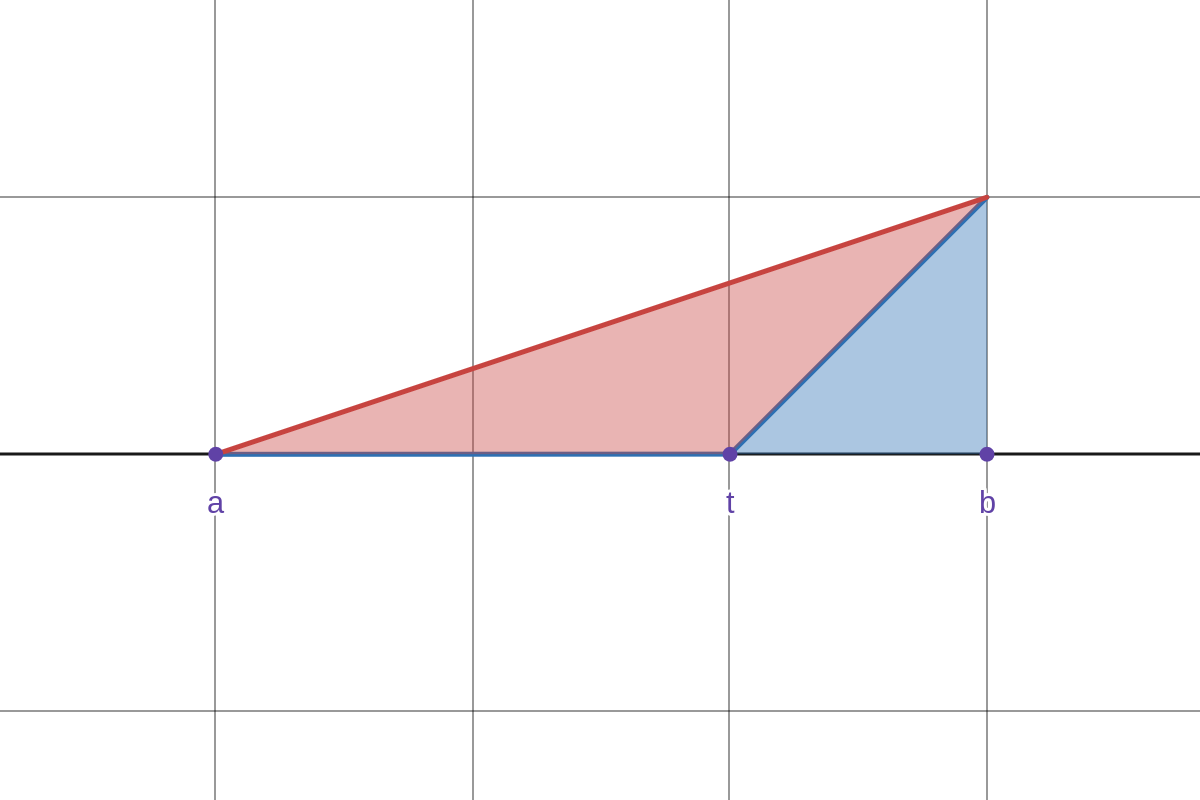
\includegraphics[scale=0.28]{../figures/peano_kernel.png}
\end{center}
che sarà chiaramente sempre $\leq 0$.

\end{minipage}

\par\smallskip

Per la formula dei trapezi vale quindi, in generale:
$$
E_1 (f) = \frac{1}{m!} f^{(m + 1)}(\varepsilon) \int_a^b G(t) \, dt = \frac{1}{m!} f^{(m + 1)}(\varepsilon) \frac{E_n(x^{m + 1})}{m + 1} = \frac{f''(\varepsilon)}{2} E_1(x^2)
$$
Preso $m = 1$.
Vediamo quindi che per $f = x^2$:
$$
E_1(x^2) = \int_a^b x^2 \, dx - \frac{b - a}{2} (a^2 + b^2) = \frac{x^3}{3} \Big|^b_a - \frac{ba^2 + b^3 - a^3 - ab^2}{2}
$$
$$
= \frac{b^3 - a^3}{3} -  \frac{ba^2 + b^3 - a^3 - ab^2}{2} = \frac{2b^3 - 2a^3 - 3ba^2 - 3b^3 + 3a^2 + 3ab^2}{6} = - \frac{(b - a)^3}{6}
$$ 
da cui:
$$
E_1(f) = - \frac{(b - a)^3}{12} \cdot f''(\varepsilon), \quad \varepsilon \in [a, b]
$$

\subsubsection{Esempio: errore di Peano nella formula di Simpson}
Si dimostra che anche la formula di Simpson è tale per cui $G(t)$ non cambia segno, quindi vale:
$$
E_2(f) = \frac{f^{(4)} (\varepsilon)}{4!} \cdot E_2(x^4) 
$$
Vediamo quindi che per l'intervallo $[-1, 1]$ vale:
$$
E_2(x^4) = \frac{2}{5} - \frac{2}{3} = - \frac{4}{15}
$$
per cui:
$$
E_2(f) = \frac{f^{(4)}(\varepsilon)}{24} \cdot \left( - \frac{4}{15} \right) = -\frac{1}{90} \cdot f^{(4)} (\varepsilon), \quad \epsilon \in [-1, 1] 
$$

Lo stesso ragionamento si può chiaramente fare per $[a, b]$ generico, cioè:
$$
E_2(x^4) = \int_{a}^{b}x^{4}dx-\frac{b-a}{6}\left(a^{4}+4\frac{\left(a+b\right)^{4}}{16}+b^{4}\right) = \frac{b^{5}-a^{5}}{5}-\frac{b-a}{24}\left(5a^{4}+4a^{3}b+6a^{2}b^{2}+4ab^{3}+5b^{4}\right)
$$
$$
= \frac{24b^{5}-24a^{5}-5\left(5a^{4}b+4a^{3}b^{2}+6a^{2}b^{3}+4ab^{4}+5b^{5}-5a^{5}-4a^{4}b-6a^{3}b^{2}-4a^{2}b^{3}-5ab^{4}\right)}{120}
$$
$$
= \frac{24b^{5}-24a^{5}-25a^{4}b-20a^{3}b^{2}-30a^{2}b^{3}-20ab^{4}-25b^{5}+25a^{5}+20a^{4}b+30a^{3}b^{2}+20a^{2}b^{3}+25ab^{4}}{120}
$$
$$
= -\frac{\left(b-a\right)^{5}}{120}
$$
da cui:
$$
E_2(f) = \frac{f^{(4)}(\varepsilon)}{24} \cdot \left( -\frac{\left(b-a\right)^{5}}{120} \right) = -\frac{(b - a)^5}{2880} \cdot f^{(4)} (\varepsilon), \quad \epsilon \in [a, b] 
$$


\subsection{Formule di quadratura interpolatorie}
Vediamo l'approccio all'approssimazione integrale che prevede scegliere $n + 1$ nodi $x_0, ..., x_n$.
In questo caso si utilizza come approssimazione di $\int_a^b f(x) \rho(x) \, dx$ la quantità:
$$
\int_a^b f(x) \rho(x) \, dx \approx \int_a^b P_n(x) \rho(x) \, dx
$$
con $P_n(x)$ polinomio di grado al più $n$ tale che:
$$
P_n(x_i) = f(x_i), \quad \forall i = 0, ..., n
$$
cioè $P_n(x)$ polinomio interpolante.

Se $f$ è sufficientemente regolare sappiamo che:
$$
f(x) = P_n(x) + R_n(x), \quad R_n(x) = \frac{\Pi (x)}{(n + 1)!} f^{(n + 1)} (\varepsilon), \quad \varepsilon \in [a, b]
$$
dal teorema 14.1.

Prendiamo quindi:
$$
\int_a^b f(x) \rho(x) \, dx = \int_a^b P_n(x) \rho(x) \, dx + \int_a^b R_n(x) \rho(x) \, dx = \int_a^b \sum_{i = 0}^n f(x_i) l_i(x) + \int_a^b R_n(x) \rho(x) \, dx
$$
dove gli $l_i(x)$ sono i polinomi della base di Lagrange:
$$
l_i(x) = \prod_{j \neq i} \frac{x - x_j}{x_i - x_j}
$$
da cui si può portare fuori la sommatoria:
$$
\int_a^b f(x) \rho(x) \, dx = \sum_{i = 0}^n f(x_i) \int_a^b l_i(x) \rho(x) \, dx + E_n(f)
$$
che ha esattamente la forma di una formula di quadratura, dove gli $f(x_i)$ sono i nodi della formula $J_n(f)$ e gli:
$$
\int_a^b l_i(x) \rho(x) \, dx
$$
a moltiplicare sono i pesi, cioè quelli che avevamo finora chiamato $a_i$.
L'errore $E_n(f)$ chiaramente si trascura.

Osserviamo che per costruzione le formule interpolatorie hanno grado di precisione almeno $n$ (chiaramente dal fatto che il polinomio interpolante di grado $n$ di un polinomio di grado $n$ è esattamente sé stesso).

Viceversa, dati $n + 1$ nodi c'è una sola formula di quadratura che ha grado di precisione $\geq n$ su qui nodi, e deve essere la formula di quadratura interpolatoria.

\subsubsection{Esempio: formule di Newton-Cotes}
L'esempio più classico delle formule di quadratura interpolatorie sono le formule di \textbf{Newton-Cotes}, che si basano sull'ipotesi di prendere nodi equispaziati su $a, b$.
Un prima scelta è riguardo all'inclusione o meno degli estremi:
\begin{itemize}
	\item Quando gli estremi $(a, b)$ sono inclusi si parla di formule di Newton-Cotes \textit{chiuse};
	\item Quando gli estremi $(a, b)$ sono esclusi si parla di formule di Newton-Cotes \textit{aperte}.
\end{itemize}

Consideriamo per adesso le formule \textbf{chiuse}, per cui:
$$
x_0 = a, \quad x_1 = h, \quad ..., \quad x_i = a + ih, \quad ..., \quad x_n = b
$$
con:
$$
h = \frac{b - a}{n}
$$
detto \textbf{passo} della formula.

I pesi $a_i$ saranno quindi:
$$
a_i = \int_a^b l_i(x) \, dx
$$

Le formule di Newton-Cotes equivalgono, per il grado 1 alle formule dei trapezi e per il grado 2 alle formule di Simosib.

Una proprietà importante delle formule di Newton-Cotes è che per ogni scelta di $n$ vale che $G(t)$ nucleo di Peano non cambia segno su $[a ,b]$, ergo si può usare la formula semplificata per l'errore di Peano:
$$
E_n(f) = \frac{f^{(m + 1)} (\varepsilon)}{(m + 1)!} \cdot E_n(x^{m + 1})
$$

Sul grado $n$ vale un fenomeno analogo al fenomeno di Runge (sezione 14.3.2).
Per $n > 7$ (cioè se si hanno più di $8$ nodi) le formule di Newton-Cotes iniziano ad avere pesi di segno alternato (mentre per $n \leq 7$ sono sempre positivi), cioè si inizia ad avere cancellazione numerica e valutare le formule diventa instabile numericamente.

\par\smallskip

Per esprimere l'errore delle formule di Newton-Cotes abbiamo quindi bisogno di trovarne l'errore $E_n(x^{m + 1})$, cioè l'errore per il monomio di grado $m + 1$ con $m$ grado di precisione.
In questo caso si assume un'espressione del tipo:
$$
E_n(f) =
\begin{cases}
	c_n \cdot h^{n + 2} \cdot f^{(n + 1)} (\varepsilon), \quad n \text{ dispari} \\			
	c_n \cdot h^{n + 3} \cdot f^{(n + 2)} (\varepsilon), \quad n \text{ pari} \\			
\end{cases}
$$

Vediamo ad esempio:
\begin{itemize}
	\item \textbf{Formula dei trapezi:} in questo caso si ha $n = 1$, $h = b - a$, da cui l'errore è esprimibile come:
		$$
		- \frac{(b - a)^3}{12} \cdot f''(\varepsilon) = -\frac{h^3}{12} \cdot f''(\varepsilon)
		$$
	\item \textbf{Formula di Simpson} in questo caso si ha $n = 2$, $h = \frac{b - a}{2}$, da cui l'errore è esprimibile come:
		$$
		- \frac{(b - a)^5}{2880} \cdot f^{(4)}(\varepsilon) = -\frac{h^5}{90} \cdot f^{(4)}(\varepsilon)
		$$
\end{itemize}

Un'altra osservazione da fare è che il grado di precisione e l'ordine della potenza di $h$ è lo stesso per una formula con grado $n$ pari e quella con grado dispari $n + 1$.
In genere, a parte il caso dei trapezi, si considerano più spesso le formule di Newton-Cotes con $n$ pari.

\par\smallskip

Vediamo nel dettaglio l'andamento del grado degli errori per qualche grado dopo lo 0.
Innanzitutto, bisogna fare una precisazione per cosa significa prendere la formula di Newton-Cotes di grado 0.
Avevamo che per formula \textit{chiusa} si intende quella che prende $n + 1$ punti estremi inclusi, mentre la formula \textit{aperta} è quella che prende $n + 1$ punti esclusi gli estremi.
Tali punti si ottengono ad esempio come:
\begin{itemize}
	\item \textbf{Formula chiusa:}
		$$
			x_i = a + i h, \quad h = \frac{b - a}{n}, \quad i = 0, 1, ..., n
		$$
	\item \textbf{Formula aperta:}
		$$
			x_i = a + (i + 1) h, \quad h = \frac{b - a}{n + 2}, \quad i = 0, 1, ..., n
		$$
\end{itemize}

Da questo risulta chiaro che sarà impossibile prendere una formula chiusa che include entrambi gli estremi quando si hanno a disposizione $n + 1 = 1$ punti per il grado $n = 0$.
Divideremo quindi fra:
\begin{itemize}
	\item \textbf{Somma di Riemann sinistra:}
		$$
			J_0^l (f) = (b - a) \cdot f(a)
		$$
	\item \textbf{Somma di Riemann destra:}
		$$
			J_0^r (f) = (b - a) \cdot f(b)
		$$
\end{itemize}

Per queste il grado è $m = 0$ e l'errore per $f = x$ risulta proporzionale al grado $2$, e non al $3$ come ci si aspetterebbe (per il punto in meno di cui non possiamo sfruttare la simmetria).
Ad esempio rispetto alla somma di Riemann sinistra si ha:
$$
E_0^l (x) = \int_a^b x \, dx - (b - a) \cdot a = \frac{b^2 - a^2}{2} - ab + a^2 = \frac{b^2 - a^2 - 2ab + 2a^2}{2} = \frac{(b - a)^2}{2}
$$

Potremo quindi considerare la formula aperta, che equivarrà alla cosiddetta \textbf{formula del punto medio}:
$$
J_0^m(f) = (b - a) \cdot f \left( \frac{a + b}{2} \right)
$$
Vediamo la particolarità che questa ha effettivamente grado $m = 1$, in quanto:
$$
E_0^m (x) = \int_a^b x \, dx - (b - a) \cdot \frac{a + b}{2} = \frac{b^2 - a^2}{2} - \frac{b^2 - a^2}{2} = 0
$$
Valutiamo quindi l'errore in $x^2$ come:
$$
E_0^m (x^2) = \frac{b^3 - a^3}{3} - (b - a) \left( \frac{a + b}{2} \right)^2 = \frac{b^3 - a^3}{3} - (b - a) \frac{a^2 + 2ab + b^2}{4}
$$
$$
= \frac{b^3 - a^3}{3} - \frac{a^2 b + 2 a b^2 b^3 - a^3 - 2 a^2 b - ab^2}{4} = \frac{b^3 - a^3}{3} + \frac{a^2 b - ab^2 - b^3 + a^3}{4}
$$
$$
= \frac{b^3 - 4a^3 + 3 a^2 b - 4 a b^2 - 3 b^3 + 3 a^3}{12} = \frac{b^3 - 3 a b^2 + 3 a^2 b - a^3}{12} = \frac{(b - a)^3}{12}
$$
cioè otteniamo un errore proporzionale a $h^3$ (lo stesso grado del metodo dei trapezi), e almeno per $x^2$ opposto a quello dato dal metodo dei trapezi.

Possiamo quindi compilare una tabella che associa i gradi di approssimazione ai gradi dell'errore per le formule di Newton-Cotes chiuse e aperte:
\begin{table}[h!]
	\center \rowcolors{2}{white}{black!10}
	\begin{tabular} { c | c | c | c | c }
		\bfseries Grado & \multicolumn{2}{c|}{\bfseries Formula} & \multicolumn{2}{c}{\bfseries Errore} \\
																		& \bfseries Aperta & \bfseries Chiusa & \bfseries Aperta & \bfseries Chiusa \\
		\hline
		0 & $(b - a) \cdot f(\frac{a + b}{2})$ & $(b - a) \cdot f(a)$ o $(b - a) \cdot f(b)$ & 3 & 2 \\ 
		1 & $ \frac{(b - a)}{2} \cdot f\left(\frac{1}{3} (2a + b) \right) + \frac{(b - a)}{2} \cdot f \left( \frac{1}{3} (a + 2b) \right)$ & $\frac{(b - a)}{2} \cdot f(a) + \frac{(b - a)}{2} \cdot f(b)$ & 3 & 3 \\
		2 & // & // & 5 & 5 \\
		3 & // & // & 5 & 5 \\
	\end{tabular}
\end{table}

\subsubsection{Esempio: formule Gaussiane}
Riprendiamo quindi anche le formule Gaussiane espresse come formule di quadratura interpolatorie.

Innanzitutto si può dire che anche per queste il nucleo di Peano $G(t)$ non cambia segno su $[a, b]$, cioè si può usare la formula di errore data dal corollario.

Un'altra proprietà è che i pesi delle formule Gaussiane sono sempre positivi, ergo non ci sono problemi di instabilità numerica per $n$ grande.

Veniamo quindi a come ricavarle.
Fissato l'intervallo $[a, b]$ e la funzione peso $\rho(x)$ si ha che le formule Gaussiane sono completamente determinate.
I nodi delle formule gaussiane si possono scrivere come zeri di particolari polinomi, detti \textit{polinomi ortogonali}.
Più precisamente sono gli zeri della successione di polinomi $\{q_n\}$, con $\deg(q_n) = n$, determinati da:
$$
< q_n, p > = 0 , \quad \forall p : \deg(p) < n
$$
sfruttando la definizione di prodotto scalare $< \cdot , \cdot >$ sullo spazio polinomiale $\mathbb{R}[x]$ data nei corsi di algebra lineare:
$$
<a, b> = \int_a^b a(x) b(x) \, dx
$$
da cui:
$$
< q_n, p > = \int_a^b q_n(x) p(x) \rho(x) \, dx
$$

\begin{itemize}
	\item
		Nel caso specifico che stavamo calcolando, con $[a, b]$ e $\rho(x) = 1$ si trova l'insieme dei \textbf{polinomi di Legendre}.
	\item 
		Usando $[a, b]$ e la funzione peso:
		$$
		\rho(x) = \frac{1}{\sqrt{1 - x^2}}
		$$
		si ottiene invece il cosiddetto \textbf{polinomio di Chebyshev di prima specie}, le cui radici sono i nodi di Chebyshev (che avevamo già incontrato nella sezione 14.3.3).
\end{itemize}

Esistono metodi ad-hoc per trovare gli zeri dei polinomi ortogonali su $[-1, 1]$. 
Una volta trovati questi si possono ottenere quelli su $[a, b]$ con il cambio di variabili:
$$
[-1, 1] \rightarrow [a, b], \quad x \rightarrow \frac{b - a}{2} x + \frac{b + a}{2}
$$
cioè una semplice operazione di scalatura lineare.

\end{document}


\documentclass[a4paper,11pt]{article}
\usepackage[a4paper, margin=8em]{geometry}

% usa i pacchetti per la scrittura in italiano
\usepackage[french,italian]{babel}
\usepackage[T1]{fontenc}
\usepackage[utf8]{inputenc}
\frenchspacing 

% usa i pacchetti per la formattazione matematica
\usepackage{amsmath, amssymb, amsthm, amsfonts}

% usa altri pacchetti
\usepackage{gensymb}
\usepackage{hyperref}
\usepackage{standalone}

% imposta il titolo
\title{Appunti Calcolo Numerico}
\author{Luca Seggiani}
\date{2025}

% disegni
\usepackage{pgfplots}
\pgfplotsset{width=10cm,compat=1.9}

% imposta lo stile
% usa helvetica
\usepackage[scaled]{helvet}
% usa palatino
\usepackage{palatino}
% usa un font monospazio guardabile
\usepackage{lmodern}

% tikz in sans
\tikzset{every picture/.style={/utils/exec={\sffamily}}}

\renewcommand{\rmdefault}{ppl}
\renewcommand{\sfdefault}{phv}
\renewcommand{\ttdefault}{lmtt}

% circuiti
\usepackage{circuitikz}
\usetikzlibrary{babel}

% disponi il titolo
\makeatletter
\renewcommand{\maketitle} {
	\begin{center} 
		\begin{minipage}[t]{.8\textwidth}
			\textsf{\huge\bfseries \@title} 
		\end{minipage}%
		\begin{minipage}[t]{.2\textwidth}
			\raggedleft \vspace{-1.65em}
			\textsf{\small \@author} \vfill
			\textsf{\small \@date}
		\end{minipage}
		\par
	\end{center}

	\thispagestyle{empty}
	\pagestyle{fancy}
}
\makeatother

% disponi teoremi
\usepackage{tcolorbox}
\newtcolorbox[auto counter, number within=section]{theorem}[2][]{%
	colback=blue!10, 
	colframe=blue!40!black, 
	sharp corners=northwest,
	fonttitle=\sffamily\bfseries, 
	title=Teorema~\thetcbcounter: #2, 
	#1
}

% disponi definizioni
\newtcolorbox[auto counter, number within=section]{definition}[2][]{%
	colback=red!10,
	colframe=red!40!black,
	sharp corners=northwest,
	fonttitle=\sffamily\bfseries,
	title=Definizione~\thetcbcounter: #2,
	#1
}

% disponi problemi
\newtcolorbox[auto counter, number within=section]{problem}[2][]{%
	colback=green!10,
	colframe=green!40!black,
	sharp corners=northwest,
	fonttitle=\sffamily\bfseries,
	title=Problema~\thetcbcounter: #2,
	#1
}

% disponi codice
\usepackage{listings}
\usepackage[table]{xcolor}

\definecolor{codegreen}{rgb}{0,0.6,0}
\definecolor{codegray}{rgb}{0.5,0.5,0.5}
\definecolor{codepurple}{rgb}{0.58,0,0.82}
\definecolor{backcolour}{rgb}{0.95,0.95,0.92}

\lstdefinestyle{codestyle}{
		backgroundcolor=\color{black!5}, 
		commentstyle=\color{codegreen},
		keywordstyle=\bfseries\color{magenta},
		numberstyle=\sffamily\tiny\color{black!60},
		stringstyle=\color{green!50!black},
		basicstyle=\ttfamily\footnotesize,
		breakatwhitespace=false,         
		breaklines=true,                 
		captionpos=b,                    
		keepspaces=true,                 
		numbers=left,                    
		numbersep=5pt,                  
		showspaces=false,                
		showstringspaces=false,
		showtabs=false,                  
		tabsize=2
}

\lstdefinestyle{shellstyle}{
		backgroundcolor=\color{black!5}, 
		basicstyle=\ttfamily\footnotesize\color{black}, 
		commentstyle=\color{black}, 
		keywordstyle=\color{black},
		numberstyle=\color{black!5},
		stringstyle=\color{black}, 
		showspaces=false,
		showstringspaces=false, 
		showtabs=false, 
		tabsize=2, 
		numbers=none, 
		breaklines=true
}

\lstdefinelanguage{javascript}{
	keywords={typeof, new, true, false, catch, function, return, null, catch, switch, var, if, in, while, do, else, case, break},
	keywordstyle=\color{blue}\bfseries,
	ndkeywords={class, export, boolean, throw, implements, import, this},
	ndkeywordstyle=\color{darkgray}\bfseries,
	identifierstyle=\color{black},
	sensitive=false,
	comment=[l]{//},
	morecomment=[s]{/*}{*/},
	commentstyle=\color{purple}\ttfamily,
	stringstyle=\color{red}\ttfamily,
	morestring=[b]',
	morestring=[b]"
}

% disponi sezioni
\usepackage{titlesec}

\titleformat{\section}
	{\sffamily\Large\bfseries} 
	{\thesection}{1em}{} 
\titleformat{\subsection}
	{\sffamily\large\bfseries}   
	{\thesubsection}{1em}{} 
\titleformat{\subsubsection}
	{\sffamily\normalsize\bfseries} 
	{\thesubsubsection}{1em}{}

% disponi alberi
\usepackage{forest}

\forestset{
	rectstyle/.style={
		for tree={rectangle,draw,font=\large\sffamily}
	},
	roundstyle/.style={
		for tree={circle,draw,font=\large}
	}
}

% disponi algoritmi
\usepackage{algorithm}
\usepackage{algorithmic}
\makeatletter
\renewcommand{\ALG@name}{Algoritmo}
\makeatother

% disponi numeri di pagina
\usepackage{fancyhdr}
\fancyhf{} 
\fancyfoot[L]{\sffamily{\thepage}}

\makeatletter
\fancyhead[L]{\raisebox{1ex}[0pt][0pt]{\sffamily{\@title \ \@date}}} 
\fancyhead[R]{\raisebox{1ex}[0pt][0pt]{\sffamily{\@author}}}
\makeatother

\begin{document}

% sezione (data)
\section{Lezione del 05-05-25}

% stili pagina
\thispagestyle{empty}
\pagestyle{fancy}

% testo
Continuiamo la trattazione dell'approssimazione di integrali attraverso le formule di quadratura interpolatorie.
Un problema che avevamo fino adesso è che se $h$ è grande, allora $E_n(f)$ è grande per qualche termine proporzionale a $h^d$, dove $d$ è il grado dell'errore.

Un'idea potrebbe essere di aumentare $n$, quindi aumentare i punti campionati per ridurre il passo $h$, ma come abbiamo visto questo è instabile (risente di fenomeni simili al fenomeno di Runge).

\subsubsection{Formule di Newton-Cotes generalizzate}
Decidiamo quindi di spezzare l'integrale su sottointervalli, e in ciascuno di essi applicare una formula di quadratura.
Questo metodo ci porterà alle formule di Newton-Cotes \textbf{generalizzate}, anche dette \textit{composite}.

Quindi, posto ad esempio un certo intervallo $[a, b]$ contenente i punti ordinati $c, d, e$, dividiamo l'integrale:
$$
\int_a^b f(x) \, dx = \int_a^c f(x) \, dx + \int_c^d f(x) \, dx + \int_d^e f(x) \, dx + \int_e^b f(x) \, dx
$$
e si applica la formula di quadratura ad ogni sottointervallo, sommando.

Più formalmente, avremo che si divide $[a, b]$ in $L$ sottointervalli equispaziati, con:
$$
x_0 = a, \quad x_1 = x_0 + \frac{b - a}{L}, \quad ..., \quad x_L = b
$$
e si divide l'integrale come:
$$
\int_a^b f(x) \, dx = \sum_{i = 1}^L \int_{x_{i - 1}}^{x_i} f(x) \, dx
$$
In ogni intervallo $[x_{i - 1}, x_i]$ si applica quindi una formula di Newton Cotes con $n + 1$ nodi.

Avremo quindi bisogno, in ogni sottointervallo, di:
$$
n + 1 - 2 = n - 1
$$ 
nodi aggiuntivi oltre agli estremi dell'intervallo per poter applicare la formula di quadratura $J_n(f)$.
Il numero di nodi totali dovrà quindi essere:
$$
L + 1 + (n - 1) \cdot L = nL + 1
$$

Osserviamo che il numero di nodi corrisponde al numero di valutazioni di $f$, e quindi in genere è un'indicazione del costo computazionale di una formula. 

\subsubsection{Esempio: formula dei trapezi generalizzata}
Prendiamo la forma che otteniamo per $n = 1$:
$$
\int_a^b f(x) \, dx \approx \sum_{i = 1}^L \frac{b - a}{2L} \left( f(x_{i - 1}) + f(x_i) \right) = \frac{b - a}{2L} \sum_{i = 1}^L \left( f(x_{i - 1}) + f(x_i) \right)
$$
$$
= \frac{b - a}{2L} \left( f(x_0) + 2 \sum_{i = 1}^{L - 1} f(x_i) + f(x_L) \right) = J_1^{(G)} (f)
$$

\subsubsection{Esempio: formula di Cavalieri-Simspon}
Vediamo quindi la generalizzazione della formula di Cavalieri, cioè ciò che otteniamo per $n = 2$:
$$
\int_a^b f(x) \, dx \approx \sum_{i = 1}^L \frac{b - a}{6L} \left( f(x_{i - 1}) + 4 f \left( \frac{x_{i - 1} + x_i}{2} \right) + f(x_i) \right)
$$
$$
= \frac{b - a}{6L} \left( f(x_0) + 2 \sum_{i = 1}^{L} f(x_i) + 4 \sum_{i = 1}^{L - 1} f\left( \frac{x_{i - 1} + x_i}{2} \right) + f(x_L) \right) = J_2^{(G)} (f)
$$

\subsubsection{Errore nelle formule generalizzate}
In ogni intervallo della forma $[x_{i - 1}, x_i]$ conosciamo l'errore, che è quello della formula di Newton-Cotes che stiamo utilizzando:
$$
e \cdot h^d \cdot f^{(d - 1)} (\varepsilon), \quad f \in C^{(d - 1)} ([a, b])
$$
L'errore sulla formula totale $J_n^{(G)}(f)$ sarà quindi:
$$
E_n^{(G)} (f) = I(f) - J_n^{(G)} (f) = \sum_{i = 1}^L c \cdot h^d \cdot f^{(d - 1)}(\varepsilon_i), \quad \varepsilon_i \in [x_{i - 1}, x_i]
$$
Vediamo quindi che l'unico termine dipendente dall'intervallo è $f^{(d - 1)} (\varepsilon)$, per cui possiamo dire:
$$
= \sum_{i = 1}^L c \cdot h^d \cdot L \frac{f^{(d - 1)}(\varepsilon_i)}{L} = c h^dL \cdot f^{(d - 1)} (\varepsilon), \quad \varepsilon \in [a, b]
$$
sfruttando il teorema della media integrale.

Abbiamo quindi gli errori:
\begin{itemize}
	\item \textbf{Formula dei trapezi:}
		$$
		E_1^{(G)}(f) = -\frac{(b - a)^3}{12L^2} \cdot f''(\varepsilon)
		$$
	\item \textbf{Formula di Cavalieri-Simpson:}
		$$
		E_2^{(G)}(f) = -\frac{(b - a)^5}{2880L^4} \cdot f^{(4)} (\varepsilon), \quad \varepsilon \in [a, b]
		$$
\end{itemize}
e il caso generale:
$$
E_n^{(G)} (f) =
\begin{cases}
	c_n \cdot \frac{(b - a)^{n + 2}}{L^{n + 1}} \cdot f^{(n + 1)} (\varepsilon), \quad n \text{ dispari} \\
	c_n \cdot \frac{(b - a)^{n + 3}}{L^{n + 2}} \cdot f^{(n + 2)} (\varepsilon), \quad n \text{ pari} \\
\end{cases}
$$

\subsection{Formule di quadratura sulle derivate}
Potremmo considerare formule di quadratura che coinvolgono le derivate di $f$.
Si possono quindi generalizzare i concetti di grado di precisione, scelta dei nodi e pesi ottimali anche per formule di quadratura del tipo:
$$
\int_a^b f(x) \rho(x) \, dx = \sum_{i = 0}^{n_1} f(x_i) + \sum_{i = 0}^{n_2} f'(y_i) + \sum_{i = 0}^{n_3} f''(z_i)
$$
chiaramente restringendo l'applicazione delle formule a funzioni sufficientemente derivabili.

Vediamo ad esempio come trovare i pesi ottimi per l'approssimazione con:
$$
\int_0^1 f(x) \, dx = I(f) \approx a_1 f(0) + a_2 f' \left( \frac{1}{3} \right) + a_3 f' \left( \frac{2}{3} \right) + f(4)
$$
sull'intervallo $[a, b] = [0, 1]$.

Imponendo errore nullo ai primi 4 gradi si otterrà:
\[
	\begin{cases}
		E_1(1)= 0 \\
		E_1(x)= 0 \\
		E_1(x^2)= 0 \\
		E_1(x^3)= 0 
	\end{cases}
	\implies
	\begin{cases}
		\int_0^1 1 \, dx = 1 = a_1 + a_4 \\ 
		\int_0^1 x \, dx = \frac{1}{2} = a_2 + a_3 + a_4 \\
		\int_0^1 x^2 \, dx = \frac{1}{3} = \frac{2}{3} a_2 + \frac{4}{3} a_3 + a_4 \\
		\int_0^1 x^3 \, dx = \frac{1}{4} = \frac{1}{3} a_2 + \frac{4}{3} a_3 + a_4
	\end{cases}
\]
Ricaviamo allora dalle prime 3:
\[
	\begin{cases}
		a_4 = 1 - a_1 \\
		a_2 = \frac{1}{2} - a_3 - a_4 \\ 
		a_3 = \frac{3}{4} \left( \frac{1}{3} - \frac{2}{3} a_2 - a_4 \right) = \frac{1}{4} - \frac{1}{2} a_2 - \frac{3}{4} a_4
\end{cases}
\]
da cui sostituendo ulteriormente:
\[
	\begin{cases}
		a_4 = 1 - a_1 \\ 
		a_2 = \frac{1}{2} + \frac{1}{2} a_4 - a_4 = \frac{1}{2} - \frac{1}{2}a_4 \\ 
		a_3 = \frac{1}{4} - \frac{1}{2} \left( \frac{1}{2} - a_3 - a_4 \right) - \frac{3}{4} a_4 = \frac{1}{2} a_3 - \frac{1}{4}a_4
	\end{cases}
\]
sostituendo tutto nella quarta si ha:
$$
\frac{1}{4} = \frac{1}{3} \left( \frac{1}{2} - \frac{1}{2} a_4 \right) + \frac{4}{3} \cdot - \frac{1}{2} a_4 + a_4 = \frac{1}{6} + \frac{1}{6} a_4 \implies a_4 \frac{1}{2} 
$$
da cui immediatamente:
$$
a_1 = \frac{1}{2}, \quad
a_2 = \frac{1}{4}, \quad
a_3 = -\frac{1}{4}, \quad
a_4 = \frac{1}{2}, \quad
$$
da cui:
$$
J_3(f) = \frac{f(0)}{2} + \frac{f' \left( \frac{1}{3} \right)}{4} - \frac{f'' \left( \frac{2}{3} \right)}{4} + \frac{f(1)}{2}
$$

Per determinare il grado di precisione vediamo l'errore per $x^4$:
$$
E_3(x^4) = \int_0^1 x^4 \, dx - \left( \frac{1}{2} \cdot 0 + \frac{1}{4} \cdot 4 \cdot \left( \frac{1}{3} \right)^3 - \frac{1}{4} \cdot 4 \cdot \left( \frac{2}{3} \right)^3 + \frac{1}{2} \right) = \frac{1}{5} - \left( \frac{1}{27} - \frac{8}{27} + \frac{1}{2} \right) = \frac{1}{5} - \frac{13}{54} \neq 0
$$
da cui il grado di precisione è esattamente 3.

\end{document}


\documentclass[a4paper,11pt]{article}
\usepackage[a4paper, margin=8em]{geometry}

% usa i pacchetti per la scrittura in italiano
\usepackage[french,italian]{babel}
\usepackage[T1]{fontenc}
\usepackage[utf8]{inputenc}
\frenchspacing 

% usa i pacchetti per la formattazione matematica
\usepackage{amsmath, amssymb, amsthm, amsfonts}

% usa altri pacchetti
\usepackage{gensymb}
\usepackage{hyperref}
\usepackage{standalone}

% imposta il titolo
\title{Appunti Calcolo Numerico}
\author{Luca Seggiani}
\date{2025}

% disegni
\usepackage{pgfplots}
\pgfplotsset{width=10cm,compat=1.9}

% imposta lo stile
% usa helvetica
\usepackage[scaled]{helvet}
% usa palatino
\usepackage{palatino}
% usa un font monospazio guardabile
\usepackage{lmodern}

% tikz in sans
\tikzset{every picture/.style={/utils/exec={\sffamily}}}

\renewcommand{\rmdefault}{ppl}
\renewcommand{\sfdefault}{phv}
\renewcommand{\ttdefault}{lmtt}

% circuiti
\usepackage{circuitikz}
\usetikzlibrary{babel}

% disponi il titolo
\makeatletter
\renewcommand{\maketitle} {
	\begin{center} 
		\begin{minipage}[t]{.8\textwidth}
			\textsf{\huge\bfseries \@title} 
		\end{minipage}%
		\begin{minipage}[t]{.2\textwidth}
			\raggedleft \vspace{-1.65em}
			\textsf{\small \@author} \vfill
			\textsf{\small \@date}
		\end{minipage}
		\par
	\end{center}

	\thispagestyle{empty}
	\pagestyle{fancy}
}
\makeatother

% disponi teoremi
\usepackage{tcolorbox}
\newtcolorbox[auto counter, number within=section]{theorem}[2][]{%
	colback=blue!10, 
	colframe=blue!40!black, 
	sharp corners=northwest,
	fonttitle=\sffamily\bfseries, 
	title=Teorema~\thetcbcounter: #2, 
	#1
}

% disponi definizioni
\newtcolorbox[auto counter, number within=section]{definition}[2][]{%
	colback=red!10,
	colframe=red!40!black,
	sharp corners=northwest,
	fonttitle=\sffamily\bfseries,
	title=Definizione~\thetcbcounter: #2,
	#1
}

% disponi problemi
\newtcolorbox[auto counter, number within=section]{problem}[2][]{%
	colback=green!10,
	colframe=green!40!black,
	sharp corners=northwest,
	fonttitle=\sffamily\bfseries,
	title=Problema~\thetcbcounter: #2,
	#1
}

% disponi codice
\usepackage{listings}
\usepackage[table]{xcolor}

\definecolor{codegreen}{rgb}{0,0.6,0}
\definecolor{codegray}{rgb}{0.5,0.5,0.5}
\definecolor{codepurple}{rgb}{0.58,0,0.82}
\definecolor{backcolour}{rgb}{0.95,0.95,0.92}

\lstdefinestyle{codestyle}{
	backgroundcolor=\color{black!5}, 
	commentstyle=\color{codegreen},
	keywordstyle=\bfseries\color{magenta},
	numberstyle=\sffamily\tiny\color{black!60},
	stringstyle=\color{green!50!black},
	basicstyle=\ttfamily\footnotesize,
	breakatwhitespace=false,         
	breaklines=true,                 
	captionpos=b,                    
	keepspaces=true,                 
	numbers=left,                    
	numbersep=5pt,                  
	showspaces=false,                
	showstringspaces=false,
	showtabs=false,                  
	tabsize=2
}

\lstdefinestyle{shellstyle}{
	backgroundcolor=\color{black!5}, 
	basicstyle=\ttfamily\footnotesize\color{black}, 
	commentstyle=\color{black}, 
	keywordstyle=\color{black},
	numberstyle=\color{black!5},
	stringstyle=\color{black}, 
	showspaces=false,
	showstringspaces=false, 
	showtabs=false, 
	tabsize=2, 
	numbers=none, 
	breaklines=true
}

\lstdefinelanguage{javascript}{
	keywords={typeof, new, true, false, catch, function, return, null, catch, switch, var, if, in, while, do, else, case, break},
	keywordstyle=\color{blue}\bfseries,
	ndkeywords={class, export, boolean, throw, implements, import, this},
	ndkeywordstyle=\color{darkgray}\bfseries,
	identifierstyle=\color{black},
	sensitive=false,
	comment=[l]{//},
	morecomment=[s]{/*}{*/},
	commentstyle=\color{purple}\ttfamily,
	stringstyle=\color{red}\ttfamily,
	morestring=[b]',
	morestring=[b]"
}

% disponi sezioni
\usepackage{titlesec}

\titleformat{\section}
{\sffamily\Large\bfseries} 
{\thesection}{1em}{} 
\titleformat{\subsection}
{\sffamily\large\bfseries}   
{\thesubsection}{1em}{} 
\titleformat{\subsubsection}
{\sffamily\normalsize\bfseries} 
{\thesubsubsection}{1em}{}

% disponi alberi
\usepackage{forest}

\forestset{
	rectstyle/.style={
		for tree={rectangle,draw,font=\large\sffamily}
	},
	roundstyle/.style={
		for tree={circle,draw,font=\large}
	}
}

% disponi algoritmi
\usepackage{algorithm}
\usepackage{algorithmic}
\makeatletter
\renewcommand{\ALG@name}{Algoritmo}
\makeatother

% disponi numeri di pagina
\usepackage{fancyhdr}
\fancyhf{} 
\fancyfoot[L]{\sffamily{\thepage}}

\makeatletter
\fancyhead[L]{\raisebox{1ex}[0pt][0pt]{\sffamily{\@title \ \@date}}} 
\fancyhead[R]{\raisebox{1ex}[0pt][0pt]{\sffamily{\@author}}}
\makeatother

\begin{document}

% sezione (data)
\section{Lezione del 09-05-25}

% stili pagina
\thispagestyle{empty}
\pagestyle{fancy}

% testo
\subsection{Approssimazione di equazioni non lineari}
Vogliamo risolvere equazioni del tipo:
$$
f(x) = 0, \quad f : \mathbb{R} \rightarrow \mathbb{R}
$$
con $f$ non lineare ($f(x) \neq ax + b$).

Osserviamo che in generale non c'è un'espressione analitica, quindi una formula chiusa, per tutti i punti $\alpha \in \mathbb{R}$ tali che $f(\alpha) = 0$, quindi che risolvono l'equazione.

Diamo quindi la definizione elementare:
\begin{definition}{Radice}
	Per un sistema $f(x) = 0$, $\alpha \in \mathbb{R}$ tale che $f(\alpha) = 0$ è detta radice o zero di $f$.
\end{definition}

Vorremo quindi cercare delle approssimazioni di $\alpha$, e più precisamente vogliamo considerare metodi numerici che generano successioni $\{x_n\}_{n \in \mathbb{N}}$ che sperabilmente hanno la proprietà:
$$
\lim_{n \rightarrow + \infty} x_n = \alpha
$$
In particolare vedremo metodi del tipo:
$$
x_{n + 1} = \phi_n (x_n, x_{n - 1}, ..., x_{n - k + 1})
$$

La funzione $\phi_n$ accetta $k$ argomenti (punti) e viene detta \textbf{funzione di iterazione}.
Se $\phi_n = \phi$, $\forall n \in \mathbb{N}$ parliamo di \textbf{metodi stazionari}.

Diamo quindi la definizione di \textbf{convergenza}:
\begin{definition}{Convergenza}
	Un metodo iterativo per risolvere $f(x)$ si dice convergente per $k$ punti iniziali $x_0, x_{-1}, ..., x_{1-k}$ se la successione generata:
	$$
	x_{n + 1} = \phi_n (x_n, x_{n - 1}, ..., x_{n - k + 1})
	$$
	verifica:
	$$
	\lim_{n \rightarrow + \infty} x_n = \alpha
	$$
	con $\alpha$ radice di $f$.
\end{definition}

Possiamo generalizzare l'idea di convergenza a convergenza \textit{di un certo ordine}:
\begin{definition}{Ordine di convergenza}
	Si dice che un metodo iterativo ha convergenza di ordine $p \geq 1$ se $\exists c < +\infty$ (costante finita), $c \neq 0$ tale per cui:
	$$
	\lim_{n \rightarrow +\infty} \frac{|x_{n + 1} - \alpha|}{|x_n - \alpha|^p} = c
	$$
	dove nel caso $p = 1$ si richiede anche $0 < c < 1$.
\end{definition}

Osserviamo quindi che la definizione dice che, asintoticamente, si ha $|e_{n + 1}| \approx |e_n|^p$.
Da questo è chiaro che se $e_{n}$ è un numero piccolo ($|e_n| \in (0, 1)$), per $p \geq 2$ (o $p = 1$ con $0 < c < 1$, come richiesto dalla definizione) $e_{n + 1}$ sarà ancora più piccolo.

In particolare si ha quindi che:
\begin{itemize}
	\item Per $p = 1$ si parla di convergenza \textbf{lineare}, cioè l'errore si riduce di un fattore $c$ ad ogni passo;
	\item Per $p = 2$ si parla di convergenza \textbf{quadratica}, e via dicendo.
\end{itemize}

Possiamo parlare di \textbf{convergenza locale}:
\begin{definition}{Convergenza locale}
	Si cha un metodo converge localmente (con ordine $p$) se $\exists S \subset \mathbb{R}$, con $\alpha \in S$, tale che per ogni scelta di $x_0, ..., x_{1 - k} \in S$, $x_n$ converge ad $\alpha$ (con ordine $p$).
\end{definition}

\subsubsection{Metodi grafici}
Riassumendo, si ha quindi che è importante saper localizzare/stimare dove sono le radici di una certa $f$ di cui ci interessa $f(x) = 0$.
Per questo scopo si possono usare strumenti di analisi del grafico di una funzione (almeno nel caso scalare):
\begin{enumerate}
	\item Se $f$ continua e $f(a) \cdot f(b) < 0 \implies \exists$ almeno una radice in $[a ,b]$ (che potrebbe essere più di una).
	\item Si può studiare la derivata, ammesso $f \in C'([a, b])$, e quindi del segno di $f$.

		\noindent
		\textbf{\textsf{Esempio}}

		Poniamo ad esempio di avere:
		$$
		f(x) = x \log(x) + \frac{1}{3}
		$$
		e di porci la domanda di trovare le radici approssimate di $f(x)$.
		Innanzitutto restringiamo il dominio a $x > 0$, e prendiamo i limiti agli estremi:
		$$
		\lim_{x \rightarrow 0^+} x \log(x) + \frac{1}{3} = \frac{1}{3}, \quad
		\lim_{x \rightarrow +\infty} x \log(x) + \frac{1}{3} = +\infty
		$$

		Prendiamo quindi la derivata:
		$$
		f'(x) = \log(x) + 1 \implies
		\begin{cases}
			f'(x) \geq 0, \quad x \geq \frac{1}{e} \\
			f'(x) \leq 0, \quad 0 < x \leq \frac{1}{e}
		\end{cases}
		$$
		e quindi $f'\left( \frac{1}{e} \right) = 0$, e la funzione descresce in $\left(0, \frac{1}{e} \right)$ per poi crescere in $\left( \frac{1}{e}, +\infty \right)$.

		Calcolando $f$ in $\frac{1}{e}$ si ha:
		$$
		f\left( \frac{1}{e} \right) = \frac{1}{e} \log\left( \frac{1}{e} \right) + \frac{1}{3} = \frac{1}{3} - \frac{1}{e} < 0
		$$
		per cui si avranno necessariamente due radici, comprese, nelle regioni:
		$$
		\alpha_1 \in \left(0, \frac{1}{e} \right), \quad \alpha_2 \in \left( \frac{1}{e}, +\infty \right)
		$$

	\item Si può procedere per separazione grafica.
		Data:
		$$
			f(x) = g(x) - h(x)
		$$
		dove $g(x)$ e $h(x)$ hano grafico noto, può essere conveniente sfruttare:
		$$
		f(x) = 0 \, \Leftrightarrow \, g(x) = h(x)
		$$
		cioè cercare i punti di intersezione fra i grafici di $g$ e $h$.
		
		\noindent
		\textbf{\textsf{Esempio}}
		
		Poniamo di avere:
		$$
		f(x) = 5x^2 - 2 e^x
		$$
		cioè:
		\[
			\begin{cases}
				h(x) = 2 e^x \\
				g(x) = 5 x^2
			\end{cases}
		\]	

		A sinistra del grafico, cioè per $\mathbb{R}^-$, ci sarà chiaramente una qualche soluzione $\alpha_1$.
		
		A destra del grafico si ha invece che $e^x$ va ad infinito più velocemente di $e^x$, cioè i grafici possono:
		\begin{enumerate}
			\item O non toccarsi mai;
			\item O toccarsi due volte (con $e^x$ che interseca $x^2$ in una fase iniziale dove va più lentamente, e quindi lo interseca di nuovo quando lo vince);
			\item O toccarsi una volta sola, come caso critico del caso precedente.
		\end{enumerate}

		Se quindi troviamo un punto $\tilde{x} \in (0, +\infty)$ dove $2e^{\tilde{x}} < 5 \tilde{x}^2$, siamo nel caso 2.
		Prendiamo allora $\tilde{x} = 2$, per cui:
		\[
			\begin{cases}
				g(2) = 20 \\
				h(2) = 2 e^2 = 2 e^2 < 2 \cdot 3^2 = 18
			\end{cases}
		\]
		per cui chiaramente avremo tre radici:
		$$
			\alpha_1 \in (-\infty, 0), \quad \alpha_2 \in (0, 2), \quad \alpha_3 \in (2, +\infty)
		$$

\end{enumerate}

\par\medskip

Iniziamo quindi a vedere i metodi iterativi veri e propri.
\subsubsection{Metodo di bisezione}
Il metodo di \textbf{bisezione} o \textit{ricerca binaria} (anche \textit{ricerca dicotomica}) consiste nel prendere un intervallo $[a, b]$ tale che $f(a) \cdot f(b) < 0$ (come nel primo esempio grafico della scorsa sezione).

In questo caso si prende come prima approssimazione:
$$
x_1 = \frac{x_0 + x_{-1}}{b}, \quad x_0 = a, \quad x_{-1} = b
$$

Si valuta quindi il segno di $f(x_1)$.
Se $f(x_1) \cdot f(x_0) < 0$, allora si scarta $b$ e si riparte con l'intervallo $[x_0, x_1]$, altrimenti si scarta $x_0$ e si riparte con l'intervallo $[x_1, x_{-1}]$.

Questo procedimento chiaramente è iterabile, e converge eventualmente ad \textit{una} radice $\alpha$, che non è detta essere l'unica.

La formula che si ottiene è la seguente:
$$
x_{n + 1} = \frac{x_{n - 1} + x_n}{2} 
$$

Per quanto riguarda l'errore (al caso \textit{idealmente} pessimo), abbiamo che questo si dimezza ad ogni passaggio:
$$
| x_{n + 1} - \alpha| < \frac{b - a}{2^n} \implies \lim_{n \rightarrow +\infty} |x_n - \alpha| = 0
$$

Questa stima è la migliore che possiamo dare, in quanto la funzione di errore $x_{n + 1} - \alpha$ non è monotona.
In ogni caso, può esserci utile a limitare l'errore con un numero minimo di passaggi al caso peggiore.

Infatti, se vogliamo:
$$
|x_n - \alpha| < t_{ol}
$$
dobbiamo usare $n$ iterazioni, con $n$ che verifica:
$$
\frac{b - a}{2^n} < t_{ol} \implies n > \log_2 \left( \frac{b - a}{t_{ol}} \right) \implies n = \left\lceil \log_2 \left( \frac{b - a}{t_{ol}} \right) \right\rceil
$$
approssimato al primo naturale superiore.

Ad esempio, se $b - a = 1$, servono $n = 10$ passi per ottenere $t_{ol} = 10^{-3}$, $n = 20$ per $t_{ol} = 10^{-6}$, e quindi in genere serviranno un numero sempre maggiore di misurazioni per ottenere precisioni migliori.

\subsubsection{Metodo delle secanti}
Il metodo delle secanti si basa su un idea geometrica, cioè quella di tracciare la \textit{retta} secante di $f$ fra $a$ e $b$, ovvero quella passante per i punti $(a, f(a))$, $(b, f(b))$.
Di questa si trova quindi l'intersezione con l'asse delle ascisse, che chiamiamo ad esempio $x_1$:
$$
x_1 = x_b - f(x_b) \cdot \frac{x_b - x_a}{f(b) - f(x_{a})}
$$
A questo punto basterà valutare il segno di $f(x_1)$ e prendere uno dei punti precedenti come per il metodo di bisezione, ed iterare finche il punto di intersezione non è abbastanza vicino ad $\alpha$.

La formula che si ottiene è la seguente:
$$
x_{n + 1} = x_n - f(x_n) \cdot \frac{x_n - x_{n - 1}}{f(x_n) - f(x_{n - 1})}
$$

Vale riguardo all'errore il seguente teorema:
\begin{theorem}{Errore del metodo delle secanti}
	Se $f \in C^2([a, b])$ ammette radice, allora il metodo converge  localmente con ordine:
	$$
		p = \frac{1 + \sqrt{5}}{2} > 1
	$$
\end{theorem}

Questo solitamente risulta in un errore migliore del lineare ma peggiore del quadratico.

\subsection{Metodi stazionari a un punto}
I \textbf{metodi stazionari a un punto} sono metodi della forma:
\[
	\begin{cases}
		x_0, \text{ dato o generato casualmente} \\
		x_{n + 1} = \phi(x_n)
	\end{cases}
\]

In questo il metodo di Jacobi e di Gauss-Seidel sono metodi stazionari a un punto.

Il modo in cui si sceglie $phi$ è (in analogia ai metodi per sistemi lineari) una funzione che verifica:
$$
\phi(\alpha) = \alpha, \quad \forall \alpha : f(\alpha) = 0
$$

Un modo canonico per costruire $\phi$ con questa proprietà è considerare:
$$
\phi(x) = x - g(x) f(x)
$$
con $g(x)$ tale che $g(x) \neq 0$ "vicino" ad $\alpha$.

Si vede che:
$$
\phi(\alpha) = \alpha - g(\alpha) f(\alpha) = \alpha
$$
e chiaramente il fatto che $g(\alpha) \neq 0$ indica che:
$$
\alpha \text{ punto fisso di $\phi$} \, \Leftrightarrow \, \alpha \text{ radice di $f$}
$$

Potremmo quindi chiederci quando $\{ \phi(x_n) \}_{n \in \mathbb{N}}$ è convergente.
Sfruttiamo per questo il seguente teorema:
\begin{theorem}{Teorema di convergenza locale}
	Se si ha un intervallo $I \subseteq \mathbb{R}$, con $\alpha \in I$, $\phi(\alpha) = \alpha$, $\phi \in C^1(I)$ e esistono $\rho \in \mathbb{R}^+$ e $k \in (0, 1)$ tali che:
	$$
	|\phi'(x)| \leq k, \quad \forall x \in [\alpha - \rho, \alpha + \rho]
	$$
	Allora valgono:
	\begin{enumerate}
		\item $\forall x_0 \in [\alpha - \rho, \alpha + \rho] \implies x_n \in [\alpha - \rho, \alpha + \rho]$;
		\item $\forall x_0 \in [\alpha - \rho, \alpha + \rho]$ si ha:
			$$
				\lim_{n \rightarrow + \infty} x_n = \alpha
			$$
		\item $\alpha$ è l'unico punto fisso di $\phi(x)$ in $[\alpha - \rho, \alpha + \rho]$.
	\end{enumerate}
\end{theorem}

Vediamo di dimostrare.
\begin{enumerate}
	\item Il punto 1) si dimostra per induzione.
		Poste le ipotesi, il caso $n = 0$ è banale (si prende lo stesso punto).
		Vogliamo quindi porre l'errore, attraverso il teorema di Lagrange:
		$$
		|x_{n + 1} - \alpha| = |\phi(x_n) - \phi(\alpha)| = |x_n - \alpha| \cdot |\phi'(\varepsilon)|, \quad \varepsilon \in [x_n, \alpha]
		$$
		di questo abbiamo che il primo termine ($|x_n - \alpha|$) è $< \rho$, e il secondo ($|\phi'(\varepsilon)|$) è $<\leq k$, per cui l'errore successivo è:
		$$
		k \rho < \rho
		$$
		cioè:
		$$
		x_{n + 1} \in [\alpha - \rho, \alpha + \rho]
		$$ 
		che è la tesi. \qed

	\item Il punto 2) si dimostra a partire dallo stesso passaggio di prima:
		$$
		|x_{n + 1} - \alpha| = |x_n - \alpha| \cdot |\phi'(\varepsilon)| \leq k |x_n - \alpha|
		$$
		maggiorando $|\phi'(\varepsilon)|$ con $k$.
		Per il calcolo esplicito si ha quindi che all'$n$-esimo passaggio si ha:
		$$
		|x_n - \alpha| \leq k^{n + 1} \cdot \rho 
		$$
		e quindi basterà dire:
		$$
		\lim_{n \rightarrow +\infty} |x_{n + 1} - \alpha| \leq \lim_{n \rightarrow  +\infty} k^{n + 1} \cdot \rho = 0 
		$$
		che è  la tesi. \qed

	\item Infine, il punto 3) si dimostra supponendo per assurdo che $\exists \tilde{\alpha} \in [\alpha - \rho, \alpha + \rho]$, $\tilde{\alpha} \neq \alpha$ tale che $\phi(\tilde{\alpha}) = \tilde{\alpha}$.
		In questo caso varrà:
		$$
		|\alpha - \tilde{\alpha}| = | \phi(\alpha) - \phi(\tilde{\alpha}) | = | \alpha - \tilde{\alpha}| \cdot | \phi'(\varepsilon) | \leq |\alpha - \tilde{\alpha} | \cdot k < | \alpha - \tilde{\alpha} |
		$$
		che guardando agli estremi è un assurdo. \qed
\end{enumerate}

Osserviamo quindi che se $|\phi'(\alpha)| < 1$, il metodo converge localmente perché per continuità della derivata $\exists \rho, k$ tali che $\rho > 0$, $k \in (0, 1)$ e $|\phi'(x)| \leq k$ $\forall x \in [\alpha - \rho, \alpha + \rho]$.

Ulteriori osservazioni si possono fare sul tipo di convergenza: questa può essere \textbf{monotona} o \textbf{alternata}.
Infatti per l'errore vale:
$$
(x_{n + 1} - \alpha) = (x_n - \alpha) \cdot \phi'(\varepsilon), \quad \varepsilon \in [x_n, \alpha]
$$

\begin{itemize}
	\item 
Se $\phi'(x) > 0$ su $[\alpha - \rho, \alpha + \rho]$, allora gli errori $x_{n + 1} - \alpha$ e $x_n - \alpha$ hanno lo stesso segno, cioè la convergenza è monotona.
	\item
		Altrimenti, se $\phi'(x) < 0$ su $[\alpha - \rho, \alpha + \rho]$, allora gli errori $x_{n + 1} - \alpha$ e $x_n - \alpha$ hanno segno discorde, cioè la convergenza è alternata.
\end{itemize}

Possiamo poi dare il seguente teorema:
\begin{theorem}{Teorema sull'ordine di convergenza}
	Sia $\phi(x) \in C^p (I)$ e $\alpha$ punto fissso di $\phi$ (cioè $\alpha = \phi(\alpha)$) con $\alpha \in I$.
	Allora $\exists \rho > 0$ tale per cui $\forall x_0 \in [\alpha - \rho, \alpha + \rho]$ la successione $\{x_n\}$ converge con ordine $p \geq 1$ ad $\alpha$ se e solo se vale:
	$$
	\phi'(\alpha) = \phi''(\alpha) = ... = \phi^{(p + 1)}(\alpha) = 0, \quad \phi^{(p)}(\alpha) \neq 0
	$$
\end{theorem}

Osserviamo che $p$ deve essere chiaramente un numero intero (un indice di derivata).

Dimostriamo quindi le due coimplicazioni.
\begin{itemize}
	\item[$\Leftarrow$:] Abbiamo che $x_{n + 1} = \phi(x_n)$. Sviluppando con Taylor nel punto $\alpha$ si ha:
		$$
		x_{n + 1} = \phi(\alpha) + \phi'(\alpha)(x_n - \alpha) + ... + \phi^{(p - 1)}(\alpha) \frac{(x_n - \alpha)^{p - 1}}{(p - 1)!} + \phi^{(p)}(\varepsilon) \frac{(x_n - a)^p}{p!}
		$$
		$$
		= \phi(\alpha) + \phi^{(p)}(\varepsilon) \frac{(x_n - \alpha)^p}{p!}, \quad \varepsilon \in [\alpha, x_n]
		$$
		Quindi:
		$$
		x_{n + 1} - \alpha = \phi^{(p)} (\varepsilon) \frac{(x_n - \alpha)^p}{p!}
		\implies
		\frac{x_{n + 1} - \alpha}{(x_n - \alpha)^p} = \frac{\phi^{(p)}(\varepsilon)}{p!} 
		$$
		$$
		\implies
		\lim_{n \rightarrow + \infty} \frac{x_{n + 1} - \alpha}{(x_n - \alpha)^p} = \lim_{n \rightarrow +\infty} \frac{\phi^{(p)}(\varepsilon)}{p!} 
		$$
		Dato che $x_n \rightarrow \alpha$, si ha che:
		$$
		\lim_{n \rightarrow +\infty} \phi^{(p)} (\varepsilon) = \phi^{(p)} (\alpha)
		$$
		e:
		$$
		\lim_{n \rightarrow +\infty} \frac{|x_{n + 1} - \alpha|}{|x_n - \alpha|^p} = \frac{\phi^{(p)} (\alpha)}{p!} \neq 0
		$$

	\item[$\Rightarrow$:] Prendiamo $1 \leq r \leq p - 1$ e facciamo vedere che:
		$$
			\phi^{(r)} (\alpha) = 0
		$$
		per induzione su $r$.

		Se $r = 1$, si ha che:
		$$
	 	\lim_{n \rightarrow +\infty} \frac{|x_{n + 1} - \alpha|}{|x_n - \alpha|} = \lim_{n \rightarrow +\infty} \frac{|\phi(x_n) - \phi(\alpha)|}{|x_n - \alpha|} = \lim_{n \rightarrow + \infty} \frac{ |x_n - \alpha| \phi'(\varepsilon) }{|x_n - \alpha|} = \phi'(\alpha)
		$$

		Prendiamo quindi per vero che $0 = \phi'(\alpha) = \phi''(\alpha) = ... = \phi^{(r - 1)} (\varepsilon)$, e dimostriamo che vale anche per $r$.
		Per fare questo prenderemo lo sviluppo di Taylor in $\alpha$ troncato all'ordine $r$:
		$$
		\phi(x_n) - \phi(\alpha) = (x_n - \alpha) \phi'(\alpha) + \frac{(x_n - \alpha)^2}{2} \phi''(\alpha) + ... + \frac{(x_n - \alpha)^{r - 1}}{(r - 1)!} \phi^{(r - 1)} (\alpha) + \frac{(x_n - \alpha)^r}{r!} \phi^{(r)} (\varepsilon)
		$$
		$$
		= \frac{(x_n - \alpha)^r}{2!} \phi^{(r)}(\varepsilon), \quad \varepsilon \in [x_n, \alpha]
		$$
		da cui:
		$$
		\frac{x_{n + 1} - \alpha}{(x_n - \alpha)^r} = \frac{\phi^{(r)} (\varepsilon)}{r!} \implies \lim_{n \rightarrow +\infty} \frac{|x_{n + 1} - \alpha|}{|x_n - \alpha|^r} = \lim_{n \rightarrow +\infty} \frac{\phi^{(r)} (\varepsilon)}{r!} = \frac{\phi^{(r)}(\alpha)}{r!} \implies \phi^{(r)}(\alpha) = 0
		$$
		\qed
\end{itemize}

\end{document}


\documentclass[a4paper,11pt]{article}
\usepackage[a4paper, margin=8em]{geometry}

% usa i pacchetti per la scrittura in italiano
\usepackage[french,italian]{babel}
\usepackage[T1]{fontenc}
\usepackage[utf8]{inputenc}
\frenchspacing 

% usa i pacchetti per la formattazione matematica
\usepackage{amsmath, amssymb, amsthm, amsfonts}

% usa altri pacchetti
\usepackage{gensymb}
\usepackage{hyperref}
\usepackage{standalone}

% imposta il titolo
\title{Appunti Calcolo Numerico}
\author{Luca Seggiani}
\date{2025}

% disegni
\usepackage{pgfplots}
\pgfplotsset{width=10cm,compat=1.9}

% imposta lo stile
% usa helvetica
\usepackage[scaled]{helvet}
% usa palatino
\usepackage{palatino}
% usa un font monospazio guardabile
\usepackage{lmodern}

% tikz in sans
\tikzset{every picture/.style={/utils/exec={\sffamily}}}

\renewcommand{\rmdefault}{ppl}
\renewcommand{\sfdefault}{phv}
\renewcommand{\ttdefault}{lmtt}

% circuiti
\usepackage{circuitikz}
\usetikzlibrary{babel}

% disponi il titolo
\makeatletter
\renewcommand{\maketitle} {
	\begin{center} 
		\begin{minipage}[t]{.8\textwidth}
			\textsf{\huge\bfseries \@title} 
		\end{minipage}%
		\begin{minipage}[t]{.2\textwidth}
			\raggedleft \vspace{-1.65em}
			\textsf{\small \@author} \vfill
			\textsf{\small \@date}
		\end{minipage}
		\par
	\end{center}

	\thispagestyle{empty}
	\pagestyle{fancy}
}
\makeatother

% disponi teoremi
\usepackage{tcolorbox}
\newtcolorbox[auto counter, number within=section]{theorem}[2][]{%
	colback=blue!10, 
	colframe=blue!40!black, 
	sharp corners=northwest,
	fonttitle=\sffamily\bfseries, 
	title=Teorema~\thetcbcounter: #2, 
	#1
}

% disponi definizioni
\newtcolorbox[auto counter, number within=section]{definition}[2][]{%
	colback=red!10,
	colframe=red!40!black,
	sharp corners=northwest,
	fonttitle=\sffamily\bfseries,
	title=Definizione~\thetcbcounter: #2,
	#1
}

% disponi problemi
\newtcolorbox[auto counter, number within=section]{problem}[2][]{%
	colback=green!10,
	colframe=green!40!black,
	sharp corners=northwest,
	fonttitle=\sffamily\bfseries,
	title=Problema~\thetcbcounter: #2,
	#1
}

% disponi codice
\usepackage{listings}
\usepackage[table]{xcolor}

\definecolor{codegreen}{rgb}{0,0.6,0}
\definecolor{codegray}{rgb}{0.5,0.5,0.5}
\definecolor{codepurple}{rgb}{0.58,0,0.82}
\definecolor{backcolour}{rgb}{0.95,0.95,0.92}

\lstdefinestyle{codestyle}{
	backgroundcolor=\color{black!5}, 
	commentstyle=\color{codegreen},
	keywordstyle=\bfseries\color{magenta},
	numberstyle=\sffamily\tiny\color{black!60},
	stringstyle=\color{green!50!black},
	basicstyle=\ttfamily\footnotesize,
	breakatwhitespace=false,         
	breaklines=true,                 
	captionpos=b,                    
	keepspaces=true,                 
	numbers=left,                    
	numbersep=5pt,                  
	showspaces=false,                
	showstringspaces=false,
	showtabs=false,                  
	tabsize=2
}

\lstdefinestyle{shellstyle}{
	backgroundcolor=\color{black!5}, 
	basicstyle=\ttfamily\footnotesize\color{black}, 
	commentstyle=\color{black}, 
	keywordstyle=\color{black},
	numberstyle=\color{black!5},
	stringstyle=\color{black}, 
	showspaces=false,
	showstringspaces=false, 
	showtabs=false, 
	tabsize=2, 
	numbers=none, 
	breaklines=true
}

\lstdefinelanguage{javascript}{
	keywords={typeof, new, true, false, catch, function, return, null, catch, switch, var, if, in, while, do, else, case, break},
	keywordstyle=\color{blue}\bfseries,
	ndkeywords={class, export, boolean, throw, implements, import, this},
	ndkeywordstyle=\color{darkgray}\bfseries,
	identifierstyle=\color{black},
	sensitive=false,
	comment=[l]{//},
	morecomment=[s]{/*}{*/},
	commentstyle=\color{purple}\ttfamily,
	stringstyle=\color{red}\ttfamily,
	morestring=[b]',
	morestring=[b]"
}

% disponi sezioni
\usepackage{titlesec}

\titleformat{\section}
{\sffamily\Large\bfseries} 
{\thesection}{1em}{} 
\titleformat{\subsection}
{\sffamily\large\bfseries}   
{\thesubsection}{1em}{} 
\titleformat{\subsubsection}
{\sffamily\normalsize\bfseries} 
{\thesubsubsection}{1em}{}

% disponi alberi
\usepackage{forest}

\forestset{
	rectstyle/.style={
		for tree={rectangle,draw,font=\large\sffamily}
	},
	roundstyle/.style={
		for tree={circle,draw,font=\large}
	}
}

% disponi algoritmi
\usepackage{algorithm}
\usepackage{algorithmic}
\makeatletter
\renewcommand{\ALG@name}{Algoritmo}
\makeatother

% disponi numeri di pagina
\usepackage{fancyhdr}
\fancyhf{} 
\fancyfoot[L]{\sffamily{\thepage}}

\makeatletter
\fancyhead[L]{\raisebox{1ex}[0pt][0pt]{\sffamily{\@title \ \@date}}} 
\fancyhead[R]{\raisebox{1ex}[0pt][0pt]{\sffamily{\@author}}}
\makeatother

\begin{document}

% sezione (data)
\section{Lezione del 12-05-25}

% stili pagina
\thispagestyle{empty}
\pagestyle{fancy}

% testo
Vediamo alcuni esempi sui medi stazionari ad un punto.

\subsubsection{Esempio: convergenza locale 1}
Prendiamo la funzione:
$$
f(x) = x \log(x) - 1
$$

Innanzitutto dimostriamo che questa ha un'unica radice nell'intervallo $[0, +\infty)$, e poi studiamo la convergenza locale dei seguenti metodi:
\begin{enumerate}
	\item L'espressione esplicita di $x$:
		$$
		\phi_1(x) = \frac{1}{\log(x)}
		$$
	\item L'espressione analoga, ma meno immediata (prendiamo la $x$ da dentro il logaritmo):
		$$
		\log(x) = \frac{1}{x} \implies \phi_2(x) = e^{\frac{1}{x}}
		$$
	\item Ciò che troveremmo applicando la formula usuale:
		$$
		\phi(x) = x - g(x) f(x) \implies \phi_3(x) = \frac{x + 1}{\log(x) + 1}
		$$
		dove $g(x)$ è:
		$$
		g(x) = \frac{1}{\log(x) + 1} 
		$$
		in quanto:
		$$
		\phi_3(x) = x - g(x) f(x) = x - \frac{x \log(x) + 1}{\log(x) + 1} = \frac{x \log(x) + 1 - x \log(x) - 1}{\log(x) + 1} = \frac{x + 1}{\log(x) + 1}
		$$
\end{enumerate}

Vediamo quindi di dimostrare l'unicità della soluzione.
Abbiamo che la derivata prima $f'(x)$ è:
$$
f'(x) = \log(x) + 1 \implies 
\begin{cases}
	f'(x) < 0, \quad x < \frac{1}{e} \\			
	f'(x) > 0, \quad x > \frac{1}{e} \\			
\end{cases}
$$
e si ha un minimo in $\frac{1}{e}$.
Vediamo quindi il limite in $0^+$:
$$
\lim_{x\rightarrow 0} x\ log(x) - 1 = -1
$$

Cioè la funzione parte da $-1$ in $x = 0$, scende fino al minimo $\frac{1}{e}$ e poi sale, incontrando l'asse delle ascisse una volta sola, nel punto $\alpha$ a cui siamo interessati.

Vorremo avere un punto $> \alpha$ per circoscrivere la regione in cui questo si trova.
Per semplificare i calcoli, proviamo $x = e$, da cui:
$$
f(e) = e \log(e) - 1 = e - 1 > 0
$$
da cui individuiamo la regione:
$$
\alpha \in \left[\frac{1}{e}, e\right]
$$

Verifichiamo quindi le convergenze dei vari metodi proposti.
\begin{enumerate}
	\item Prendiamo la derivata:
		$$
		\phi_1'(x) = \left( \frac{1}{\log(x)} \right)' = \frac{1}{x} \left( - \frac{1}{\log^2(x)} \right) = - \frac{1}{x \log^2(x)}
		$$
		e valutiamone il modulo in $\alpha$:
		$$
		|\phi_1'(\alpha)| = \left| \frac{1}{\alpha \log^2(\alpha)} \right| = \left| \frac{1}{\log(\alpha)} \right| = |\alpha| \in \left[\frac{1}{e}, e\right]
		$$
		sfruttando $\alpha \log(\alpha) = 1$.

		Abbiamo quindi che $\alpha$ è potenzialmente grande fino a $e$, quindi non convergente.
		Per convincercene, prendiamo il punto 1:
		$$
		f(1) = \log(1) - 1 = -1
		$$
		da cui sicuramente, in quanto $f(\alpha)$ sarà $0 > -1$ e quindi $\alpha > 1$:
		$$
		|\phi_1'(\alpha)| > 1
		$$
		e il metodo non converge.

	\item Prendiamo la derivata:
		$$
		\phi_2'(x) = \left( e^{\frac{1}{x}} \right)' = -\frac{1}{x^2} e^{\frac{1}{x}} 
		$$
		e valutiamone il modulo in $\alpha$:
		$$
		|\phi_2'(\alpha)| = \left| -\frac{\alpha}{\alpha^2} \right| = -\frac{1}{\alpha}
		$$
		sfruttando $\alpha = e^{\frac{1}{\alpha}}$.
		
		Da questo abbiamo che:
		$$
		|\phi_2'(\alpha)| < 1
		$$
		in quanto $\alpha \in [1, e]$, e quindi il metodo converge localmente, in modo lineare ($\phi_2'(\alpha) \neq 0$).

	\item Prendiamo la derivata:
		$$
		\phi_3'(x) = \left( \frac{x + 1}{\log(x) + 1} \right)' = \frac{( \log(x) + 1) - (x + 1) \frac{1}{x}}{(\log(x) + 1)^2} = \frac{\log(x) - \frac{1}{x}}{(\log(x) + 1)^2}
		$$
		$$
		= \frac{x \log(x) - 1}{x (\log(x) + 1)^2} = \frac{f(x)}{x (\log(x) + 1)^2}
		$$
		da cui si ha $f(x)$ al denominatore, e quindi sicuramente:
		$$
		\phi_3'(\alpha) = 0
		$$
		e si converge con ordine maggiore o uguale al lineare.
		
		Vediamo la derivata seconda per confermare l'ordine di convergenza:
		$$
		\phi_3''(x) = \frac{ (\log(x) + 1)^3 x - (x \log(x) - 1) \left[ (\log(x) + 1)^2 + \frac{2(\log(x) + 1)}{x} \right] }{ x^2 (\log(x) + 1)^4 } 
		$$
		che sostituendo $\alpha$ diventa:
		$$
		\phi_3''(\alpha) = \frac{\alpha (\log(\alpha) + 1)^3}{\alpha^2 (\log(\alpha + 1)^4)} = \frac{1}{\alpha (\log(\alpha) + 1)} \neq 0
		$$
		cioè l'ordine di convergenza è 2.
\end{enumerate}

\subsubsection{Esempio: convergenza locale 2}
Prendiamo adesso un esempio dove ci è data la funzione di punto fisso: 
$$
\phi(x) = 1 + a \log(x) + b \log^2(x), \quad a, b \in \mathbb{R}
$$
con punto fisso $\alpha = 1$.
Siamo interessati a valutarne l'ordine di convergenza al variare dei parametri $a$ e $b$, e determinare quando la convergenza è lineare e monotona.
Prendiamo quindi la derivata:
$$
\phi'(x) = \frac{a}{x} + 2b \frac{\log(x)}{x} \implies \phi'(1) = a
$$
e il metodo converge localmente per $a \in (-1, 1)$.
In particolare, il metodo converge in modo monotono (localmente) quando $a \in (0, 1)$, e per $a = 0$ converge in modo superlineare.

Valutiamo quindi l'ordine di convergenza per $a = 0$:
$$
\phi(x) = 1 + b \log^2(x)
$$
da cui le derivate:
$$
\phi'(x) = 2b \frac{\log(x)}{x} \implies \phi'(\alpha) = 0
$$
$$
\phi''(x) = \frac{2b}{x^2} - 2b \frac{\log(x)}{x^2} = 2b \frac{(1 - \log(x))}{x^2} \implies \phi''(1) = 2b
$$
cioè per $b \neq 0$ la convergenza è quadratica, e per $b = 0$ la convergenza è in un passo ($x_1 = \alpha = 1$ per ogni $x_0$).

Nel caso $a = 0$ per studiare la convergenza monotona dobbiamo studiare il segno di $\phi'(x)$ vicino ad $\alpha = 1$.
\begin{itemize}
	\item[$b > 0$:] vale $\phi'(x) > 0$ su $(1, 1 + \rho)$ con $\rho$ sufficientemente piccolo, quindi si ha convergenza monotona con $x_0 \in (1, 1 + \rho)$.
	\item[$b < 0$:] vale $\phi'(x) > 0$ su $(1 - \rho, 1)$ con $\rho$ sufficientemente piccolo, quindi si ha convergenza monotona con $x_0 \in (1 - \rho, 1)$.
\end{itemize}

\subsection{Metodo di Newton}
Vediamo un particolare metodo stazionario ad un punto, cioè il \textbf{metodo di Newton}:
$$
\phi(x) = x - \frac{f(x)}{f'(x)}
$$
e quindi il passo iterativo è:
\[
	\begin{cases}
		x_0, \quad \text{dato}	\\
		x_{n + 1} = \phi(x_n) =  x_n - \frac{f(x_n)}{f'(x_n)}
	\end{cases}
\]

L'interpretazione geometrica del metodo di Newton è quella classica, cioè si prende la retta tangente che si stacca da $x_i$ e si chiama $x_{i + 1}$ l'intersezione di questa con l'asse delle ascisse. 
Per questo viene detto anche \textit{metodo delle tangenti}.

Il metodo di Newton è solitamente molto veloce, ma può presentare comporamenti non ottimali nel caso di funzioni particolarmente \textit{"schiacciate"}, cioè con derivata $|f'(x)| << 1$ vicino ad $\alpha$, fra cui ad esempio le polinomiali $x^n$ con $n >> 1$.

Per valutare questi punti sfavorevoli diamo la definizione di \textbf{radice di ordine} $\mathbf{r}$:
\begin{definition}{Radice di ordine $\mathbf{r}$}
	Sia $f : [a, b] \rightarrow \mathbb{R}$ continua e $\alpha : f(\alpha) = 0$.
	In questo caso $\alpha$ è detta radice (o zero) di ordine $r > 0$ se vale:
	$$
		\lim_{x \rightarrow \alpha} \frac{f(x)}{(x - \alpha)^r} = c < + \infty \ (c \neq 0)
	$$
\end{definition}
Quindi, se $f(x) \in C^r([a, b])$, allora $\alpha$ è radice di ordine $r$ se:
$$
f(\alpha) = f'(\alpha) = ... = f^{(r - 1)}(\alpha) = 0, \quad f^{(r)} (\alpha) \neq 0
$$
In particolare, se $r = 1$, la radice si dice \textbf{semplice}.

Riguardo al teorema di Newton, vale quindi il teorema:
\begin{theorem}{Convergenza del metodo di Newton}
	Se $\alpha$ è radice semplice, e $f \in C^2([a, b])$, allora il metodo converge localmente con ordine $p \geq 2$.
\end{theorem}
In particolare varrà:
$$
	\lim_{n \rightarrow +\infty} \frac{|x_{n + 1} - \alpha|}{|x_n - \alpha|^2} = \frac{1}{2} \frac{f''(\alpha)}{f'(\alpha)}
$$
per cui:
\[
	\begin{cases}
		f''(\alpha) = 0 \implies p > 2 \\
		f''(\alpha) \neq 0 \implies p = 2
	\end{cases}
\]

Vediamo di dimostrare il teorema.
Inizieremo prendendo la funzione di punto fisso:
$$
\phi(x) = x - \frac{f(x)}{f'(x)} \implies \phi'(x) = 1 - \frac{(f'(x))^2 - f (x) f''(x)}{(f'(x))^2} = \frac{f(x) f''(x)}{(f'(x))^2}
$$
che sostituendo $\alpha$ diventa:
$$
\phi'(\alpha) = \frac{f(\alpha) f''(\alpha)}{(f'(\alpha))^2} = 0
$$
per cui la convergenza è almeno quadratica.

Continuando si ha:
$$
\phi''(x) = \frac{( f'(x) f''(x) + f(x) f'''(x) ) (f'(x))^2 - f(x) f''(x) ( 2f'(x) f''(x) ) }{(f'(x))^4}
$$
che sostituendo $\alpha$ diventa:
$$
\phi''(\alpha) = \frac{f'(\alpha) f''(\alpha) \left( f'(\alpha) \right)^2 }{ ( f'(\alpha) )^4 } = \frac{f''(\alpha)}{f'(\alpha)}
$$
da cui:
\[
	\begin{cases}
		f''(\alpha) \neq 0 \implies p = 2 \\
		f''(\alpha) = 0 \implies p > 2
	\end{cases}
\]

In particolare, si può prendere:
$$
\frac{|x_{n + 1} - \alpha|}{|x_n - \alpha|^2} = \frac{|\phi(x_n) - \phi(\alpha)|}{|x_n - \alpha|^2} 
= \frac{ | \phi(\alpha) + \phi'(\alpha) (x_n - \alpha) + \frac{1}{2} \phi''(\varepsilon) (x_n - \alpha)^2 - \phi(\alpha) | }{ |x_n - \alpha|^2 }
$$
sfruttando lo sviluppo di Taylor di $\phi(x_n)$ attorno a $\alpha$ con errore di Laplace:
$$
\phi(x_n) = \pphi(\alpha) + \phi'(\alpha) (x_n - \alpha) + \frac{1}{2} \phi''(\alpha) (x_n - \alpha)^2
$$
da cui:
$$
= \frac{ | \phi'(\alpha) (x_n - \alpha) + \frac{1}{2} \phi''(\varepsilon) (x_n - \alpha)^2 | }{ |x_n - \alpha|^2 }
= \frac{1}{2} \phi''(\varepsilon) \xrightarrow{n \rightarrow +\infty} \frac{1}{2} \phi''(\alpha) = \frac{1}{2} \frac{f''(\alpha)}{f'(\alpha)}
$$
con $n \rightarrow +\infty$, noto $\varepsilon \in [x_n, \alpha]$, per cui si ha l'ultima tesi del teorema. \qed

Osserviamo che nel metodo di Newton si può guardare direttamente a $f(x)$ e alle sue derivate in $\alpha$ per studiare la convergenza del metodo.
Con i generici metodi di punto fisso dovevamo invece guardare alla funzione di punto fisso $\phi(x)$.

Vediamo quindi il caso delle radici multiple, cioé $f(x)$ in forma:
$$
f(x) = g(x) (x - \alpha)^r, \quad g(\alpha) \neq 0
$$

Si ha che $r \in \mathbb{N}$, $r > 1$ e:
$$
f'(\alpha) = 0
$$
e quindi il metodo di newton si ridefinisce come:
$$
\phi(x) =
	\begin{cases}
		x - \frac{f(x)}{f'(x)}, \quad x \neq \alpha \\ 
		\alpha,  \quad x = \alpha
	\end{cases}
$$

Ricordiamo che:
$$
\phi'(x) = 1 - \frac{(f'(x))^2 - f(x) f''(x)}{(f'(x))^2} = \frac{f(x) f''(x)}{(f'(x))^2}
$$
dove $f'(x)$ compare al denominatore, quindi non si può valutare in $\alpha$.

Prendiamo allora le derivate successive di $f(x)$:
\begin{enumerate}
	\item 
$
f(x) = g(x) (x - \alpha)^r
$
	\item 
$
f'(x) = g'(x) (x - \alpha)^r + r g(x) (x - \alpha)^{r - 1} = (x - \alpha)^{r - 1} ( g'(x)(x - \alpha) + r g(x) )
$
	\item
$
f''(x) = g''(x) (x - \alpha)^r + 2 r g'(x)(x - \alpha)^{r - 1} + r (r - 1) g(x) (x - \alpha)^{r - 1}
$ \\ 
$$
= (x - \alpha)^{r - 2} ( g''(x) (x - \alpha)^2 + 2 r g'(x) (x - \alpha) + r (r - 1) g(x) )
$$
\end{enumerate}
e sostituiamo in $\phi'(x)$:
$$
\phi'(x) = \frac{ g(x) (x - \alpha)^r \cdot (x - \alpha)^{r - 2} ( g''(x) (x - \alpha^2) + r g'(x) (x - \alpha) + r (r - 1) g(x) ) }{ ( (x - \alpha)^{r - 1} (g'(x) (x - \alpha) + r g(x) ) )^2 }
$$
$$
= \frac{g(x) (g''(x) (x - \alpha^2) + 2 r g'(x) (x - \alpha) + r^2 g^2(x) - r g^2(x) }{(g'(x)(x - \alpha) + r g(x))^2}
$$
da cui:
$$
\phi'(\alpha) = \frac{r^2 g^2(\alpha) - r g^2(\alpha)}{r^2 g^2(\alpha)} = 1 - \frac{1}{r} \neq 0
$$
quando $r > 1$, perciò:
$$
|\phi'(\alpha)| = 1 - \frac{1}{r} < 1
$$
e la convergenza è lineare, dove più è alto $r$ più è lenta la convergenza.

Una proprietà è che se si conosce $r$ (l'ordine della radice) si può modificare Newton per ritrovare la convergenza quadratica.
In particolare si può dimostrare che:
$$
x_{n + 1} = x_n - r \cdot \frac{f(x_n)}{f'(x_n)} = \phi(x_n)
$$
è tale per cui $\phi'(\alpha) = 0$, e quindi la convergenza è almeno quadratica.

\end{document}


\documentclass[a4paper,11pt]{article}
\usepackage[a4paper, margin=8em]{geometry}

% usa i pacchetti per la scrittura in italiano
\usepackage[french,italian]{babel}
\usepackage[T1]{fontenc}
\usepackage[utf8]{inputenc}
\frenchspacing 

% usa i pacchetti per la formattazione matematica
\usepackage{amsmath, amssymb, amsthm, amsfonts}

% usa altri pacchetti
\usepackage{gensymb}
\usepackage{hyperref}
\usepackage{standalone}

% imposta il titolo
\title{Appunti Calcolo Numerico}
\author{Luca Seggiani}
\date{2025}

% disegni
\usepackage{pgfplots}
\pgfplotsset{width=10cm,compat=1.9}

% imposta lo stile
% usa helvetica
\usepackage[scaled]{helvet}
% usa palatino
\usepackage{palatino}
% usa un font monospazio guardabile
\usepackage{lmodern}

% tikz in sans
\tikzset{every picture/.style={/utils/exec={\sffamily}}}

\renewcommand{\rmdefault}{ppl}
\renewcommand{\sfdefault}{phv}
\renewcommand{\ttdefault}{lmtt}

% circuiti
\usepackage{circuitikz}
\usetikzlibrary{babel}

% disponi il titolo
\makeatletter
\renewcommand{\maketitle} {
	\begin{center} 
		\begin{minipage}[t]{.8\textwidth}
			\textsf{\huge\bfseries \@title} 
		\end{minipage}%
		\begin{minipage}[t]{.2\textwidth}
			\raggedleft \vspace{-1.65em}
			\textsf{\small \@author} \vfill
			\textsf{\small \@date}
		\end{minipage}
		\par
	\end{center}

	\thispagestyle{empty}
	\pagestyle{fancy}
}
\makeatother

% disponi teoremi
\usepackage{tcolorbox}
\newtcolorbox[auto counter, number within=section]{theorem}[2][]{%
	colback=blue!10, 
	colframe=blue!40!black, 
	sharp corners=northwest,
	fonttitle=\sffamily\bfseries, 
	title=Teorema~\thetcbcounter: #2, 
	#1
}

% disponi definizioni
\newtcolorbox[auto counter, number within=section]{definition}[2][]{%
	colback=red!10,
	colframe=red!40!black,
	sharp corners=northwest,
	fonttitle=\sffamily\bfseries,
	title=Definizione~\thetcbcounter: #2,
	#1
}

% disponi problemi
\newtcolorbox[auto counter, number within=section]{problem}[2][]{%
	colback=green!10,
	colframe=green!40!black,
	sharp corners=northwest,
	fonttitle=\sffamily\bfseries,
	title=Problema~\thetcbcounter: #2,
	#1
}

% disponi codice
\usepackage{listings}
\usepackage[table]{xcolor}

\definecolor{codegreen}{rgb}{0,0.6,0}
\definecolor{codegray}{rgb}{0.5,0.5,0.5}
\definecolor{codepurple}{rgb}{0.58,0,0.82}
\definecolor{backcolour}{rgb}{0.95,0.95,0.92}

\lstdefinestyle{codestyle}{
	backgroundcolor=\color{black!5}, 
	commentstyle=\color{codegreen},
	keywordstyle=\bfseries\color{magenta},
	numberstyle=\sffamily\tiny\color{black!60},
	stringstyle=\color{green!50!black},
	basicstyle=\ttfamily\footnotesize,
	breakatwhitespace=false,         
	breaklines=true,                 
	captionpos=b,                    
	keepspaces=true,                 
	numbers=left,                    
	numbersep=5pt,                  
	showspaces=false,                
	showstringspaces=false,
	showtabs=false,                  
	tabsize=2
}

\lstdefinestyle{shellstyle}{
	backgroundcolor=\color{black!5}, 
	basicstyle=\ttfamily\footnotesize\color{black}, 
	commentstyle=\color{black}, 
	keywordstyle=\color{black},
	numberstyle=\color{black!5},
	stringstyle=\color{black}, 
	showspaces=false,
	showstringspaces=false, 
	showtabs=false, 
	tabsize=2, 
	numbers=none, 
	breaklines=true
}

\lstdefinelanguage{javascript}{
	keywords={typeof, new, true, false, catch, function, return, null, catch, switch, var, if, in, while, do, else, case, break},
	keywordstyle=\color{blue}\bfseries,
	ndkeywords={class, export, boolean, throw, implements, import, this},
	ndkeywordstyle=\color{darkgray}\bfseries,
	identifierstyle=\color{black},
	sensitive=false,
	comment=[l]{//},
	morecomment=[s]{/*}{*/},
	commentstyle=\color{purple}\ttfamily,
	stringstyle=\color{red}\ttfamily,
	morestring=[b]',
	morestring=[b]"
}

% disponi sezioni
\usepackage{titlesec}

\titleformat{\section}
{\sffamily\Large\bfseries} 
{\thesection}{1em}{} 
\titleformat{\subsection}
{\sffamily\large\bfseries}   
{\thesubsection}{1em}{} 
\titleformat{\subsubsection}
{\sffamily\normalsize\bfseries} 
{\thesubsubsection}{1em}{}

% disponi alberi
\usepackage{forest}

\forestset{
	rectstyle/.style={
		for tree={rectangle,draw,font=\large\sffamily}
	},
	roundstyle/.style={
		for tree={circle,draw,font=\large}
	}
}

% disponi algoritmi
\usepackage{algorithm}
\usepackage{algorithmic}
\makeatletter
\renewcommand{\ALG@name}{Algoritmo}
\makeatother

% disponi numeri di pagina
\usepackage{fancyhdr}
\fancyhf{} 
\fancyfoot[L]{\sffamily{\thepage}}

\makeatletter
\fancyhead[L]{\raisebox{1ex}[0pt][0pt]{\sffamily{\@title \ \@date}}} 
\fancyhead[R]{\raisebox{1ex}[0pt][0pt]{\sffamily{\@author}}}
\makeatother

\begin{document}

% sezione (data)
\section{Lezione del 16-05-25}

% stili pagina
\thispagestyle{empty}
\pagestyle{fancy}

% testo

\subsection{Intervallo di convergenza}
Vorremo estendere la definizione di convergenza data in 19.2 in un certo intervello $[a, b]$.

Iniziamo con un esempio:
\subsubsection{Esempio: convergenza del metodo di Newton}
Prendiamo la funzione:
$$
f(x) = 3 x^2 e^{-x} - 1
$$
e poniamo:
$$
f(x) = 0
$$
cioè equivalentemente uguagliamo le due funzioni:
$$
3x^2 = e^x
$$
che sono rispettivamente una parabola simmetrica rispetto all'asse $y$ e un esponenziale.

Queste intersezioni saranno 3, che chiamiamo $\alpha_{1, 2, 3}$.
Avremo che, scelti i punti $x_{0, 1, 2}$:
$$
x_0 = -\frac{1}{2}, \quad x_1 = 1, \quad x_2 = 5
$$
si avrà la convergenza nei rispettivi punti $\alpha_{1, 2, 3}$.

\subsubsection{Convergenza in un intervallo}
Una domanda che potremo farci, in relazione all'ultimo esempio, è quando possiamo assicurare che un metodo converge $\forall x_0 \in [a, b]$.

Esiste il seguente teorema:
\begin{theorem}{Teorema di convergenza in un intervallo}
	Se $\phi(x) \in C^1 ([a, b])$ e:
	\begin{enumerate}
		\item $|\phi'(x)| < 1, \quad \forall x \in [a, b]$;
		\item $\phi(x) \in [a, b], \quad \forall x \in [a, b]$;
	\end{enumerate}
	allora $\phi(x)$ converge su $[a, b]$.
\end{theorem}
Dove l'ipotesi in più rispetto al teorema di convergenza locale (teorema 19.2) è la 2.

\subsubsection{Condizioni di convergenza globale per Newton}
Nello specifico per Newton, la convergenza in un intervallo si assicura attraverso condizioni su concavità e convessità.

Esiste infatti il seguente teorema:
\begin{theorem}{Convergenza globale per Newton}
	Se $\alpha \in [a, b]$ è radice semplice di $f \in C^2([a, b])$, e $f, f''$ sono di segno costante su $[a, b]$, il metodo di Newton converge globalmente in maniera superlineare ($\geq 2$) $\forall x_0$ che verifica:
	$$
	f(x_0) \cdot f''(x_0) > 0
	$$
\end{theorem}
Dove si mette enfasi su \textit{globalmente}, in quanto il teorema 20.1 ha valenza solo locale.
Sostanzialmente, questo teorema ci è utile per fare stime iniziali, probabilmente arbitrariamente distanti dall'origine, che convergano con velocità superlinare.

Osserviamo che:
\begin{itemize}
	\item Se la funzione è \textbf{concava}, chiediamo $f(x_0) < 0$;
	\item Se la funzione è \textbf{convessa}, chiediamo $f(x_0) > 0$.
\end{itemize}

In particolare distinguiamo quindi i 4 casi:
\begin{enumerate}
	\item $f' > 0$, $f'' > 0$ convessa crescente, vorremo partire a \textit{destra} di $\alpha$;
	\item $f' < 0$, $f'' > 0$ convessa decrescente, vorremo partire a \textit{sinistra} di $\alpha$;
	\item $f' > 0$, $f'' < 0$ concava crescente, vorremo partire a \textit{sinistra} di $\alpha$;
	\item $f' < 0$, $f'' < 0$ concava decrescente, vorremo partire a \textit{destra} di $\alpha$;
\end{enumerate}

Cioè riassumendo:
\begin{table}[H]
	\center 
	\begin{tabular} { c | c c }
		& $f'(x) > 0$ & $f'(x) < 0$ \\
		\hline
		$f''(x) > 0$      
		&
		\raisebox{-\totalheight}{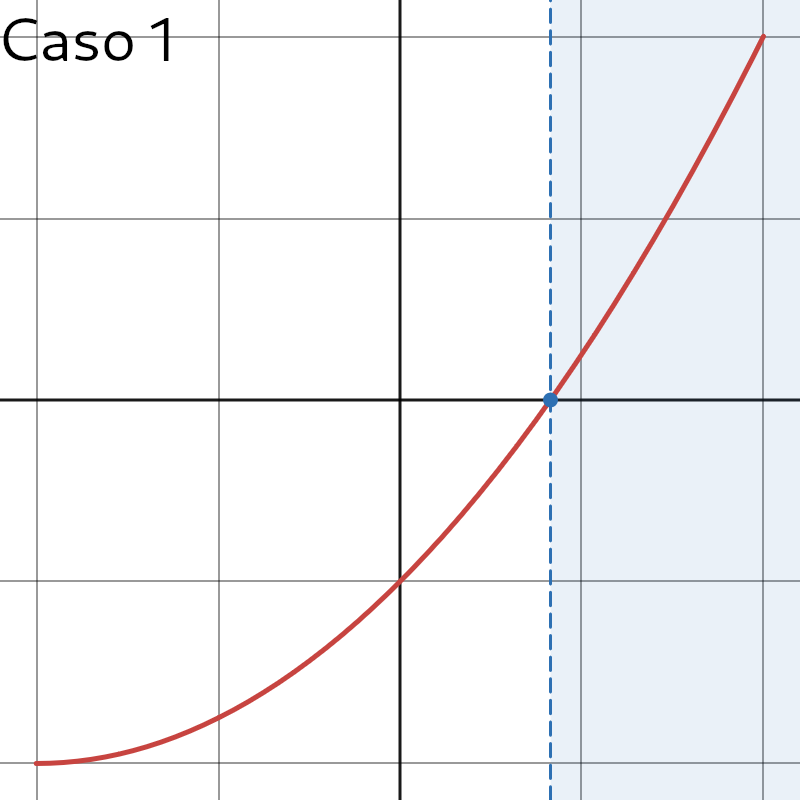
\includegraphics[scale=0.2]{../figures/newton_conv/case_1.png}} 
		& 
		\raisebox{-\totalheight}{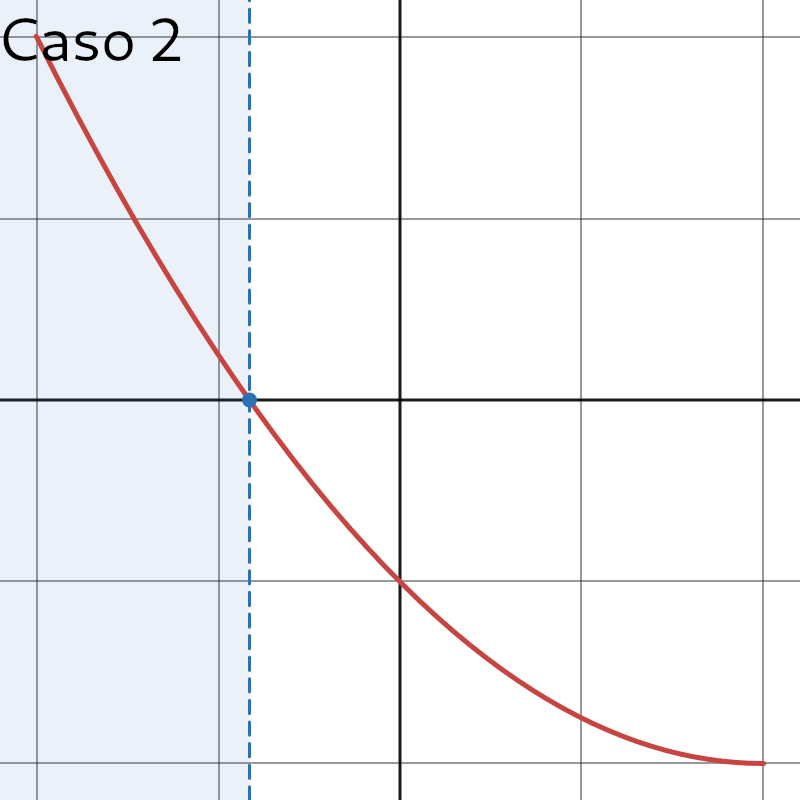
\includegraphics[scale=0.2]{../figures/newton_conv/case_2.png}} 
		\\
		$f''(x) < 0$
		&
		\raisebox{-\totalheight}{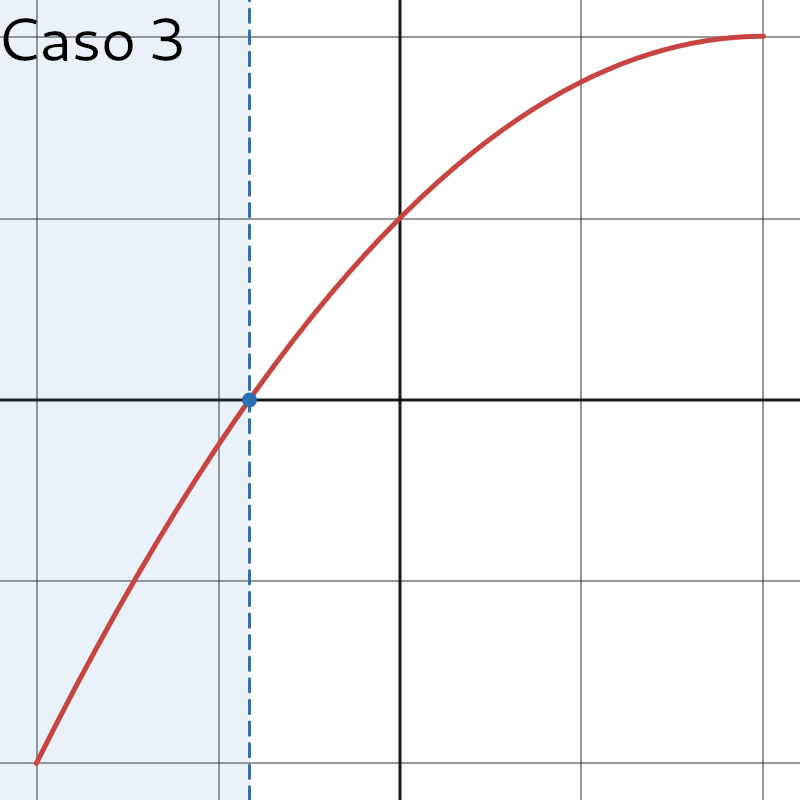
\includegraphics[scale=0.2]{../figures/newton_conv/case_3.png}} 
		& 
		\raisebox{-\totalheight}{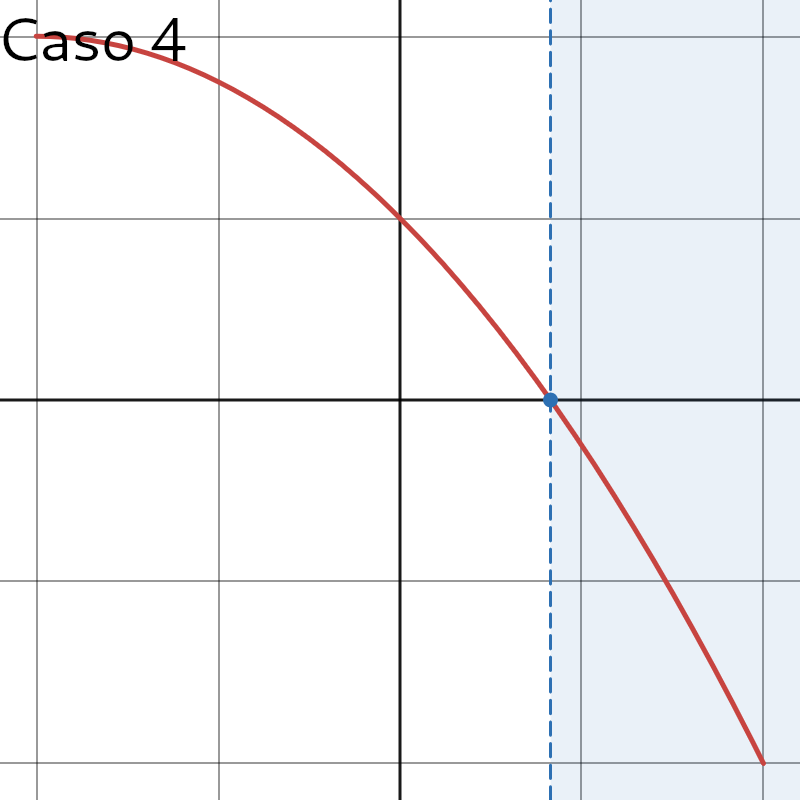
\includegraphics[scale=0.2]{../figures/newton_conv/case_4.png}} 
		\\
	\end{tabular}
\end{table}

\subsubsection{Esempio: ricerca di un intervallo di convergenza}
Prendiamo la funzione:
$$
f(x) = x + \log(x)
$$
e cerchiamo un intervallo dove questa ha una radice, in particolare fornendo un punto di partenza $x_0$ per cui Newton risulta convergente.

Chiaramente quello che cerchiamo sono le intersezioni dei grafici:
$$
\log(x) = -x
$$
che saranno una sola, compresa fra 0 e 1, perciò:
$$
\alpha \in (0, 1)
$$

Vediamo quindi se si applicano le condizioni di convergenza per Newton.
Calcoliamo innanzitutto le derivate:
$$
f'(x) = 1 + \frac{1}{x}, \quad > 0 \text{ su } (0, 1)
$$
$$
f''(x) = -\frac{1}{x^2}, \quad < 0 \text{ su } (0, 1)
$$

Per $1$ la condizione non è soddisfatta, in quanto si troverà a \textit{destra} di $\alpha$ (e trovandoci nel caso 3, vorremo prendere punti a \textit{sinistra}).

Dovremo quindi cercare un $x_0 \in (0, \alpha)$, ovvero $x_0 : f(x_0) < 0$.
Proviamo $\frac{1}{e}$:
$$
f\left(\frac{1}{e}\right) = \frac{1}{e} - 1 < 0
$$
per cui possiamo scegliere $x_0 = \frac{1}{e}$ ed essere sicuri, per il teorema 21.2, di convergere ad $\alpha$.

\subsubsection{Esempio: miglioramento della convergenza con Newton}
Avevamo visto nell'esempio 20.1.1 come Newton poteva dare convergenza non ottimale per alcuni valori.

In particolare, avevamo preso la funzione:
$$
f\left(x\right)=\left(x-3\right)^{4}-2
$$
e stavamo cercando la radice fra $3$ e $5$.
Notiamo che in questo intervallo $f''(x) > 0$, e qundi vogliamo partire da un punto $x_0$ tale per cui $f(x_0) > 0$. 
Prendiamo ad esempio $5$, con $f(5) = 14$:
\begin{lstlisting}[language=MATLAB, style=codestyle]	
>> newton_method(f, 5)

Iteration 1
	x: 5.0000

Iteration 2
	x: 4.5625

Iteration 3
	x: 4.3029

Iteration 4
	x: 4.2033

Iteration 5
	x: 4.1895

ans =

    4.1892
\end{lstlisting}
dove notiamo che troviamo una soluzione in sole 5 iterazioni, contro le 25 di cui avevamo avuto bisogno partendo da $x_0 = 3.1$ nell'esempio precedente.

\subsection{Equazioni non lineari in $\mathbb{R}^m$}
Vediamo quindi di considerare sempre equazioni non lineari, ma in più variabili (in particolare $m$).

Cercheremo quindi $f(x) = 0$ per $f: \mathbb{R}^m \rightarrow \mathbb{R}^m$, cioè:
$$
f =
\begin{pmatrix}
	f_1 (x_1, ..., x_m) \\
	\vdots \\
	f_m (x_1, ..., x_m) \\
\end{pmatrix}
$$
e vorremo trovare $\alpha \in \mathbb{R}^m$, cioè:
$$
\alpha = 
\begin{pmatrix}
	\alpha_1 \\
	\vdots \\
	\alpha_m
\end{pmatrix}
$$
tale che:
$$
f(\alpha) = 
\begin{pmatrix}
	f_1 (\alpha_1, ..., \alpha_m) \\
	\vdots \\
	f_m (\alpha_1, ..., \alpha_m) \\
\end{pmatrix}
= 0
$$

Questo problema corrisponde effettivamente a cercare soluzioni a sistemi di $m$ equazioni in $m$ incognite, non lineari.

\par\smallskip

In particolare, ci può essere utile per trovare i punti stazionari di funzioni in più variabili, ovvero le soluzioni di $\nabla F(x) = 0$, con $F(x) : \mathbb{R}^m \rightarrow \mathbb{R}$ cioè:
$$
\nabla F(x) = 
\begin{pmatrix}
	\frac{\partial }{\partial x_1} F(x_1, ..., x_m) \\
	\vdots \\ 
	\frac{\partial }{\partial x_m} F(x_1, ..., x_m) \\
\end{pmatrix}
$$

\par\smallskip

Nel caso dei sistemi lineari, avevamo la condizione semplice:
$$
f(x) = b - Ax, \quad x = A^{-1} b
$$
mentre in questo caso non avremo a disposizione tali semplificazioni.

Ci potremo quindi chiedere come risolvere $f(x)$ nel caso non lineare.
La soluzione sarà quella di generalizzare i metodi di punto fisso a $\mathbb{R}^m$, definendoli come:
$$
x = \phi(x), \quad \phi : \mathbb{R}^m \rightarrow \mathbb{R}^m
$$
e quindi usare la solita formula di aggiornamento:
$$
x^{(n + 1)} = \phi(x^{(n)})
$$

Una possibile formula di aggiornamento può essere:
$$
\phi(x) = x - G(x) \cdot f(x)
$$
dove $G(x)$ è:
$$
G(x) : \mathbb{R}^m \rightarrow \mathbb{R}^{m \times m}
$$
cioè:
$$
G(x) =
\begin{pmatrix}
	G_{11}(x) & ... & G(1m)(x) \\
	\vdots & \vdots & \vdots \\
	G_{m1}(x) & ... & G(mm)(x) \\
\end{pmatrix}
$$
e si cerca $G(x)$ tale che $G(\alpha)$ è non singolare, ovvero 
$$
\det(G(\alpha)) \neq 0
$$
Quindi si considera l'iterazione:
\[
	\begin{cases}
		x^{(0)} \in \mathbb{R}^m, \quad \text{dato} \\
		x^{(n + 1)} = x^{(n)} - G(x^{(n)}) f(x^{(n)}) = \phi (x^{(n)})
	\end{cases}
\]

Ridiamo la definizione di convergenza in $\mathbb{R}^n$:
\begin{definition}{Convergenza multivariabile}
	La successione $\{x^{(n)}\}_{n \in \mathbb{N}}$ converge ad $\alpha \in \mathbb{R}^m$ se:
	$$
	\lim_{n \rightarrow + \infty} | x^{(n)} - \alpha|_2 = 0
	$$
\end{definition}

In particolare, la convergenza ha \textbf{ordine} $p > 0$ se vale:
$$
\lim_{n \rightarrow +\infty} \frac{|x^{(n + 1)} - \alpha|_2}{|x^{(n)} - \alpha|_2^p} = c 
$$
con $c \neq 0$, $c < +\infty$, e in particolare nel caso $p = 1$ è $C \in (0, 1)$, cioè si ha la stessa situazione della definizione 19.3.

\par\smallskip

Nel caso esistano e siano continue le derivate delle componenti di $\phi(x)$ si introduce il \textbf{Jacobiano} di $\phi$, come la funzione $J_\phi : \mathbb{R}^m \rightarrow \mathbb{R}^{m \times m}$ definita da:
$$
J_\phi(x) = 
\begin{pmatrix}
	\frac{\partial \phi_1}{\partial x_1}(x) & ... & \frac{\partial \phi_1}{\partial x_m}(x) \\
	\vdots & \vdots & \vdots \\
	\frac{\partial \phi_m}{\partial x_1}(x) & ... & \frac{\partial \phi_m}{\partial x_m}(x) \\
\end{pmatrix}
$$
oppure per componenti:
$$
[J_\phi(x)]_{ij} = \frac{\partial \phi_i}{\partial x_j} (x), \quad i, j = 1, ..., m
$$

Potremo quindi enunciare il seguente teorema:
\begin{theorem}{Convergenza locale multivariabile}
	Sia $\phi(x) \in C^1(\Omega)$, $\Omega \subseteq \mathbb{R}^m$ con $\alpha \in \Omega$ tale che $\phi(\alpha) = \alpha$.
	Se:
	$$
	\rho\left(J_\phi (\alpha) \right) < 1
	$$
	cioè il raggio spettrale del Jacobiano di $\phi$ in $\alpha$ è $< 1$, allora $\exists \delta > 0$ tale che:
	$$
	\forall x^{(0)} : |x^{(0)} - \alpha|_2 < \delta
	$$
	in cui la successione:
	$$
	x^{(n + 1)} = \phi(x^{(n)})
	$$
	converge ad $\alpha$, ed $\alpha$ è l'unico punto fisso di $\phi$ in:
	$$
	\{ z \in \mathbb{R}^m : |z - \alpha|_2 < \delta \}
	$$
\end{theorem}

Osserviamo quindi che se per una qualsiasi norma si trova che:
$$
| J_\phi(\alpha) | < 1
$$
allora vale la tesi del teorema, ovvero la convergenza locale.
Viceversa, se si trova che:
$$
| J_\phi(\alpha) | \geq 1
$$
non si può concludere nulla.

\subsubsection{Esempio: convergenza multivariabile}
Prendiamo la funzione, con $m = 2$:
$$
f(x_1, x_2) = 
\begin{pmatrix}
	x_1 - \frac{1}{4} (x_1^2 + x_2^2) \\
	x_2 + x_1 - 2
\end{pmatrix}
$$
e cerchiamone i punti $f(\alpha) = 0$, cioè che soddisfano:
\[
	\begin{cases}
		x_1 - \frac{1}{4} (x_1^2 + x_2^2) = 0 \\
		x_2 + x_1 - 2 = 0
	\end{cases}
\]

Dalla $f$, posto $f(x) = 0$ si derivano le identità:
\[
	\begin{cases}
		x_1 = \frac{1}{4} (x_1^2 + x_2^2)	\\
		x_2 = 2 - x_1
	\end{cases}
\]
per cui si può considerare $\phi(x)$:
$$
\phi(x) =
\begin{pmatrix}
	\frac{1}{4} (x_1^2 + x_2^2) \\
	2 - x_1
\end{pmatrix}
$$
e 
prendere l'aggiornamento dal metodo stazionario ad un punto:
$$
x^{(n + 1)} = \phi(x^{(n)})
$$

\par\smallskip

Prima di valutare la convergenza, cerchiamo di trovare i punti $\alpha$ in maniera analitica.

Per la prima equazione, avremo che:
$$
x - \frac{1}{4} (x^2 + y^2) = 0 \, \Rightarrow \, - \frac{(x - 2)^2}{4} - \frac{y^2}{4} + 1 = 0
$$
cioè si trova la circonferenza di centro $(2, 0)$ e raggio $2$.

Per la seconda, si ha invece semplicemente la retta:
$$
y = 2 - x
$$

Sul grafico, questo ha l'aspetto:
\begin{center}
	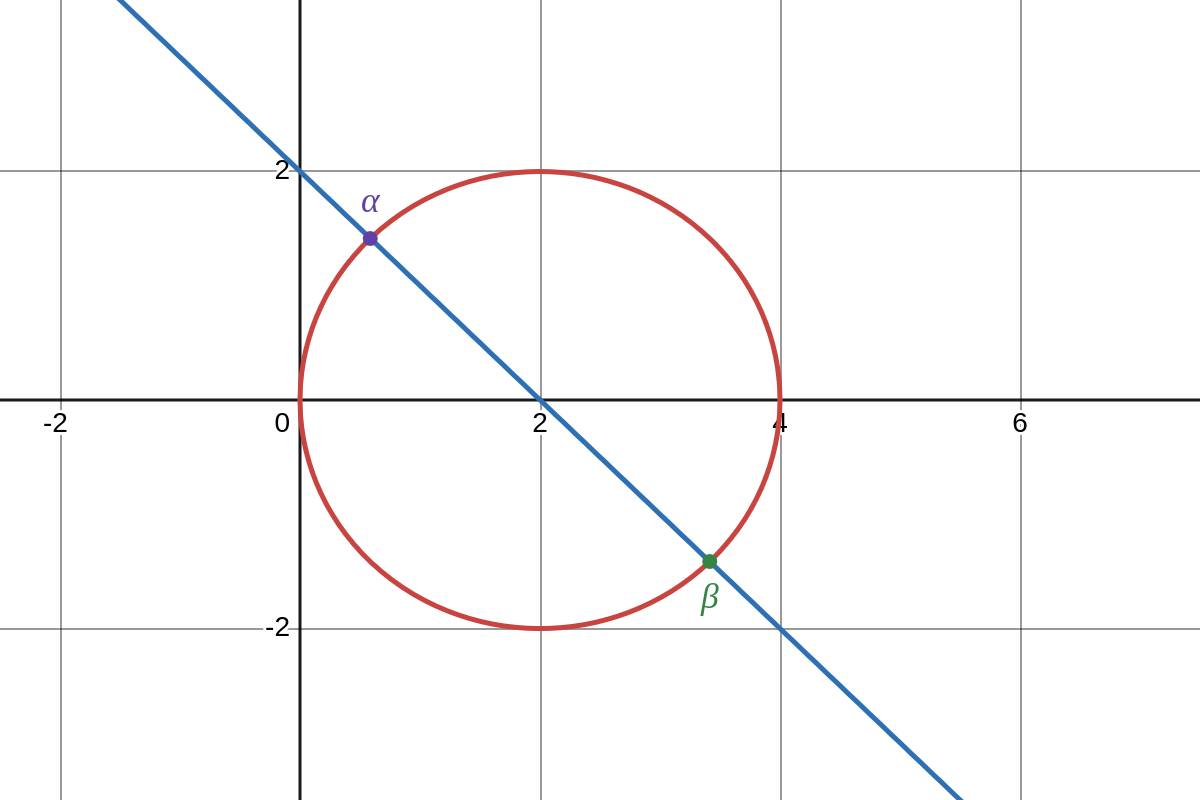
\includegraphics[scale=0.3]{../figures/nonlin.png}
\end{center}

Le soluzioni di $f(x) = 0$ saranno quindi i punti di intersezione fra la circonferenza e la retta, che vediamo essere 2, uno sopra l'asse $x$ e l'altro sotto.
Consideriamone solo il primo, che chiamiamo $(\alpha_1, \alpha_2)$.

\par\smallskip

Calcoliamo quindi il Jacobiano:
$$
J_\phi(x) =
\begin{pmatrix}
	\frac{x_1}{2} & \frac{x_2}{2} \\
	-1 & 0
\end{pmatrix}
$$

Vediamo che questa ha norma $\geq 1$, per cui bisogna calcolare gli autovalori.

Guardiamo quindi al polinomio caratteristico:
$$
\left(\frac{x_1}{2} - \lambda\right) \left(-\lambda\right) + \frac{x_2}{2} = \lambda^2 - \frac{x_1}{2} \lambda + \frac{x_2}{2} \rightarrow \lambda_{1, 2} = \frac{\frac{x_1}{2} \pm \sqrt{\frac{x_1^2}{4} - 2 x_2}}{2}
$$
cioè:
$$
\lambda_{1, 2} = \frac{\frac{\alpha_1}{2} \pm \sqrt{\frac{\alpha_1^2}{4} - 2 \alpha_2}}{2}
$$

Valutando la posizione generica di $\alpha$, si ha che:
$$
\alpha_1 < 1, \quad \alpha_2 \in (1, 2)
$$
che formalmente si ottiene notando che $\alpha_1 \geq 1$ porta ad un assurdo, e $\alpha_2 = 2 - \alpha_1$.

Da questo deriverà che il discriminante:
$$
\Delta = \frac{\alpha_1^2}{4} - 2 \alpha_2 < 0
$$
e cioè $\lambda_{1, 2}^\alpha$ sono necessariamente numeri complessi in forma:
$$
\lambda_{1, 2}^\alpha = \frac{\alpha_1}{4} \pm i \sqrt{ \frac{\alpha_2}{2} - \frac{\alpha_1^2}{16} }
$$

Il modulo di uno di questi (prendiamo il primo) sarà:
$$
|\lambda_1^\alpha|^2 = \frac{\alpha_1^2}{16} + \frac{\alpha_1}{2} - \frac{\alpha_1^2}{16} = \frac{\alpha_1}{2}
$$
per cui il raggio spettrale sarà $\frac{\alpha_1}{2} < 1$ (dal fatto che $\alpha_1 < 1$), e quindi il metodo convergente.

\subsubsection{Esempio: convergenza multivariabile con MATLAB}
Facciamo una trattazione meno analitica e più numerica della convergenza nello scorso esempio.

Avevamo individuato due radici, chiamiamole $\alpha$ (già ampiamente discussa) e $\beta$.
Queste si calcono esplicitamente prendendo dalla seconda equazione:
$$
x_2 + x_1 - 2 = 0 \implies x_2 = 2 - x_1
$$
e sostituendo nella prima:
$$
x_1 - \frac{1}{4} (x_1^2 + (2 - x_1)^2) = -\frac{x_1^2}{2} + 2 x_1 - 1
$$
da cui:
$$
\alpha = (2 - \sqrt{2}, \sqrt{2}), \quad \beta = (2 + \sqrt{2}, - \sqrt{2})
$$

Potremo chiaramente rifare le stesse considerazioni di prima con i valori effettivi di $\alpha$, trovando gli stessi risultati.
Ci basti sapere che il punto $\alpha$ fa (come avevamo visto) da attrattore, mentre il metodo non converge in $\beta$, scelto l'aggiornamento:
$$
\phi(x) =
\begin{pmatrix}
	\frac{1}{4} (x_1^2 + x_2^2) \\
	2 - x_1
\end{pmatrix}
$$

Vediamo di implementare in MATLAB un risolutore che applichi nella pratica tale funzione.
Questo si tradurrà nel dire:
\lstset{style=codestyle, language=MATLAB}
\lstinputlisting{../code/matlab/nonlin_r2_ex.m}

Dove notiamo che si stampano alcune informazioni intermedie sui punti attraversati, e si traccia il percorso seguito su un grafico.

\begin{itemize}
	\item Se si sceglie come punto di inizio $(1, 1)$, con l'intenzione di convergere ad $\alpha$, si ha il seguente andamento:
		\begin{center}
			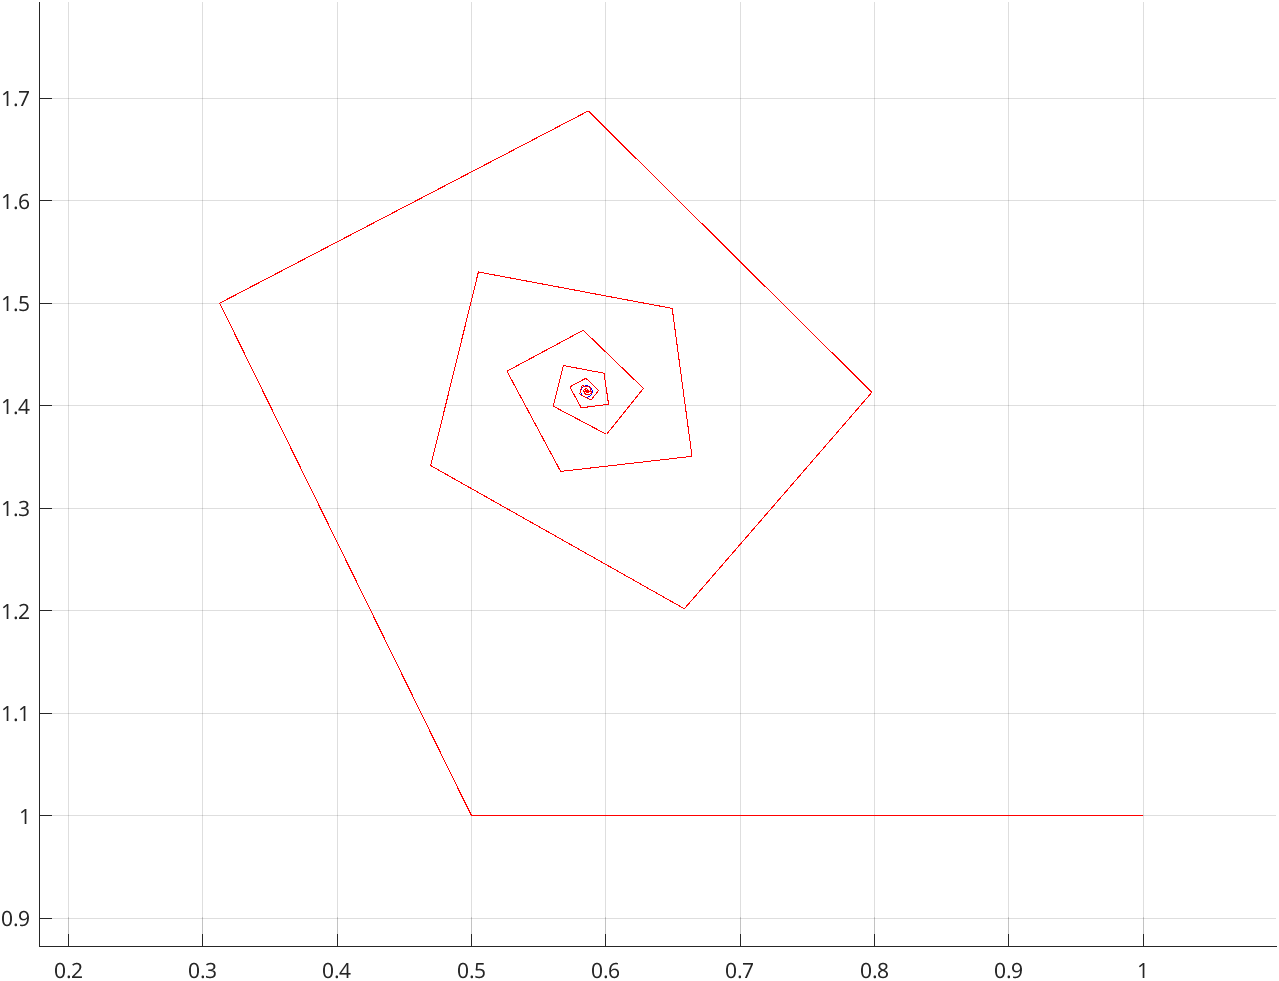
\includegraphics[scale=1]{../figures/nonlin_ex.png}
		\end{center}
		da dove si nota chiaramente che in un numero limitato di passaggi ci si avvicina abbastanza velocmente ad $\alpha$;
		\newpage
	\item Cercare di fare la stessa cosa ad esempio dal punto $(4, -1)$ non dà risultati simili, in quanto notiamo dal grafico:
		\begin{center}
			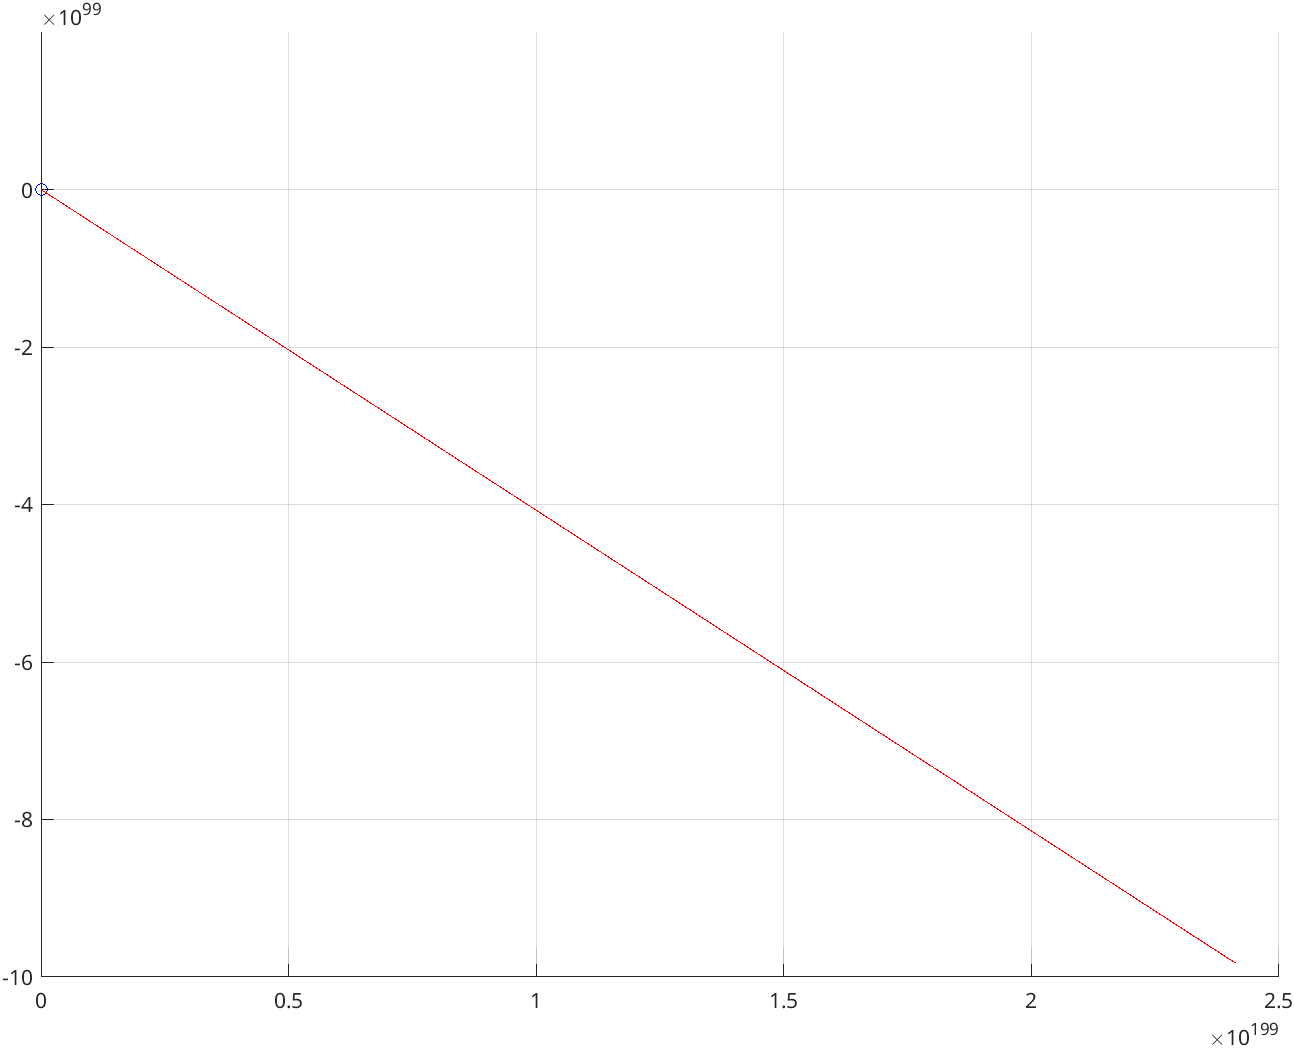
\includegraphics[scale=1]{../figures/nonlin_ex2.png}
		\end{center}
		che il risultato esplode velocemente all'infinito, e quindi chiaramente il metodo non converge.
\end{itemize}

\subsection{Metodo di Newton-Raphson}
Vediamo quindi la versione multivariabile del metodo di Newton-Raphson.

Quindi, se abbiamo $f : \mathbb{R}^m \rightarrow \mathbb{R}^m$ il metodo di Newton si generalizza nel seguente modo:
$$
x^{(n + 1)} = x^{(n)} - J_f (x^{(n)})^{-1} f(x^{(n)})
$$

Osserviamo che ad ogni passo si valuta $J_f(x^{(n)})$ e $f(x^{(n)})$, si risolve il sistema lineare:
$$
J_f(x^{(n)}) y = f(x^{(n)})
$$
ed infine si chiama $x^{(n + 1)} = x^{(n)} - y$.

L'aggiornamento complessivo sarà quindi:
\[
	\begin{cases}
		x^{(0)}, \quad \text{dato} \\
		x^{(n + 1)} = x^{(n)} - J_f(x^{(n)})^{-1} f(x^{(n)})
	\end{cases}
\]

Per quanto riguarda la convergenza si ha il seguente risultato:
\begin{theorem}{Convergenza del metodo di Newton-Rapson}
	Sia $f \in C^2(\Omega)$, $\Omega \subseteq \mathbb{R}^m$, $\alpha \in \Omega$ tale che $f(\alpha) = 0$.
	Se $J_f(\alpha)$ è non singolare, allora $\exists s \subseteq \Omega$ intorno di $\alpha$ tale che $\forall x^{(0)} \in S$ la successione generata dal metodo di Newton-Raphson a partire da $x^{(0)}$ converge e vale:
	$$
	|x^{(n + 1)} - \alpha|_2 \leq \beta |x^{(n)} - \alpha |_2^2
	$$
	ovvero la convergenza è almeno quadratica (quindi superlineare).
\end{theorem}

\subsubsection{Esempio: convergenza del metodo di Newton-Raphson}
Vediamo quindi come valutare la convergenza del metodo di Newton-Raphson per il sistema:
$$
f(x_1, x_2) =
\begin{pmatrix}
	\frac{1}{3} (x_1 - x_2) + x_1^2 \\
	\frac{1}{3} (-x_1 + x_2) + x_1 x_2
\end{pmatrix}
$$

\par\smallskip

Vogliamo quindi determinare le radici di $f$, che si otterrano come:
\[
	\begin{cases}
		\frac{x_1 - x_2}{3} + x_1^2 = 0 \\
		\frac{x_2 - x_1}{3} + x_1 x_2 = 0
	\end{cases}
	\, \Rightarrow \,
	\begin{cases}
		x_2 = 3 x_1^2 + x_1 \\
		\left( \frac{- x_1 + x_1 + 3 x_1^2}{3} \right) + x_1 (3 x_1^2 + x_1) = 0
	\end{cases}
	\, \Rightarrow \,
	\begin{cases}
		x_2 = 3 x_1^2 + x_1 \\
		2x_1^2 + 3x_1^3 = 0
	\end{cases}
\]
da cui si ottengono i due punti:
$$
\alpha = \begin{pmatrix}
0 \\ 0
\end{pmatrix}, \quad
\beta = \begin{pmatrix}
	-\frac{2}{3} \\ \frac{2}{3}
\end{pmatrix}
$$

\par\smallskip

Vorremo quindi valutare il Jacobiano:
$$
J_f(x_1, x_2) =
\begin{pmatrix}
	\frac{1}{3} + 2 x_1 & -\frac{1}{3} \\
	-\frac{1}{3} + x_2 & \frac{1}{3} + x_1
\end{pmatrix}
$$

Che nei due punti $\alpha$ e $\beta$ risulta:
\begin{itemize}
	\item[$\alpha$]:
		$$
		J_f(\alpha) =
		\begin{pmatrix}
			\frac{1}{3} & -\frac{1}{3} \\ 
			-\frac{1}{3} & \frac{1}{3}
		\end{pmatrix}
		$$
		da cui $\det = 0$, e la convergenza non è superlineare;
	\item[$\beta$]:
		$$
		J_f(\beta) =
		\begin{pmatrix}
			-1 & -\frac{1}{3} \\ 
			\frac{1}{3} & -\frac{1}{3}
		\end{pmatrix}
		$$
		da cui $\det \neq 0$, e la convergenza è superlineare;
\end{itemize}

\subsubsection{Esempio: convergenza del metodo di Newton-Raphson con MATLAB}
Vediamo di confermare quanto abbiamo detto sopra sfruttando uno strumento di calcolo.
Potrebbe venirci in mente di "colorare" su un grafico le regioni che convergono nei punti $\alpha$ e $\beta$, e di valutarne la velocità di convergenza.

\newpage

Iniziamo con un implementazione del metodo di Newton-Raphson che sfrutta il risolutore di MATLAB per essere il più veloce possibile:
\begin{lstlisting}[language=MATLAB, style=codestyle]	
function [x0, i] = q_nraph(x0)
		for i = 1:100
				f0 = f_handle(x0);
				j0 = j_handle(x0);

				% solve j0 y = f0
				y0 = j0 \ f0;
				x1 = x0 - y0;

				if norm(x1 - x0) < 0.01
						break;
				end

				x0 = x1;
		end
end
\end{lstlisting}
e usiamo quindi le funzioni per la colorazione di grafici che MATLAB offre:
\lstinputlisting{../code/matlab/raphson_ex.m}

\newpage

L'esecuzione di questo script ci fornisce in pochi secondi il seguente grafico:
\begin{center}
	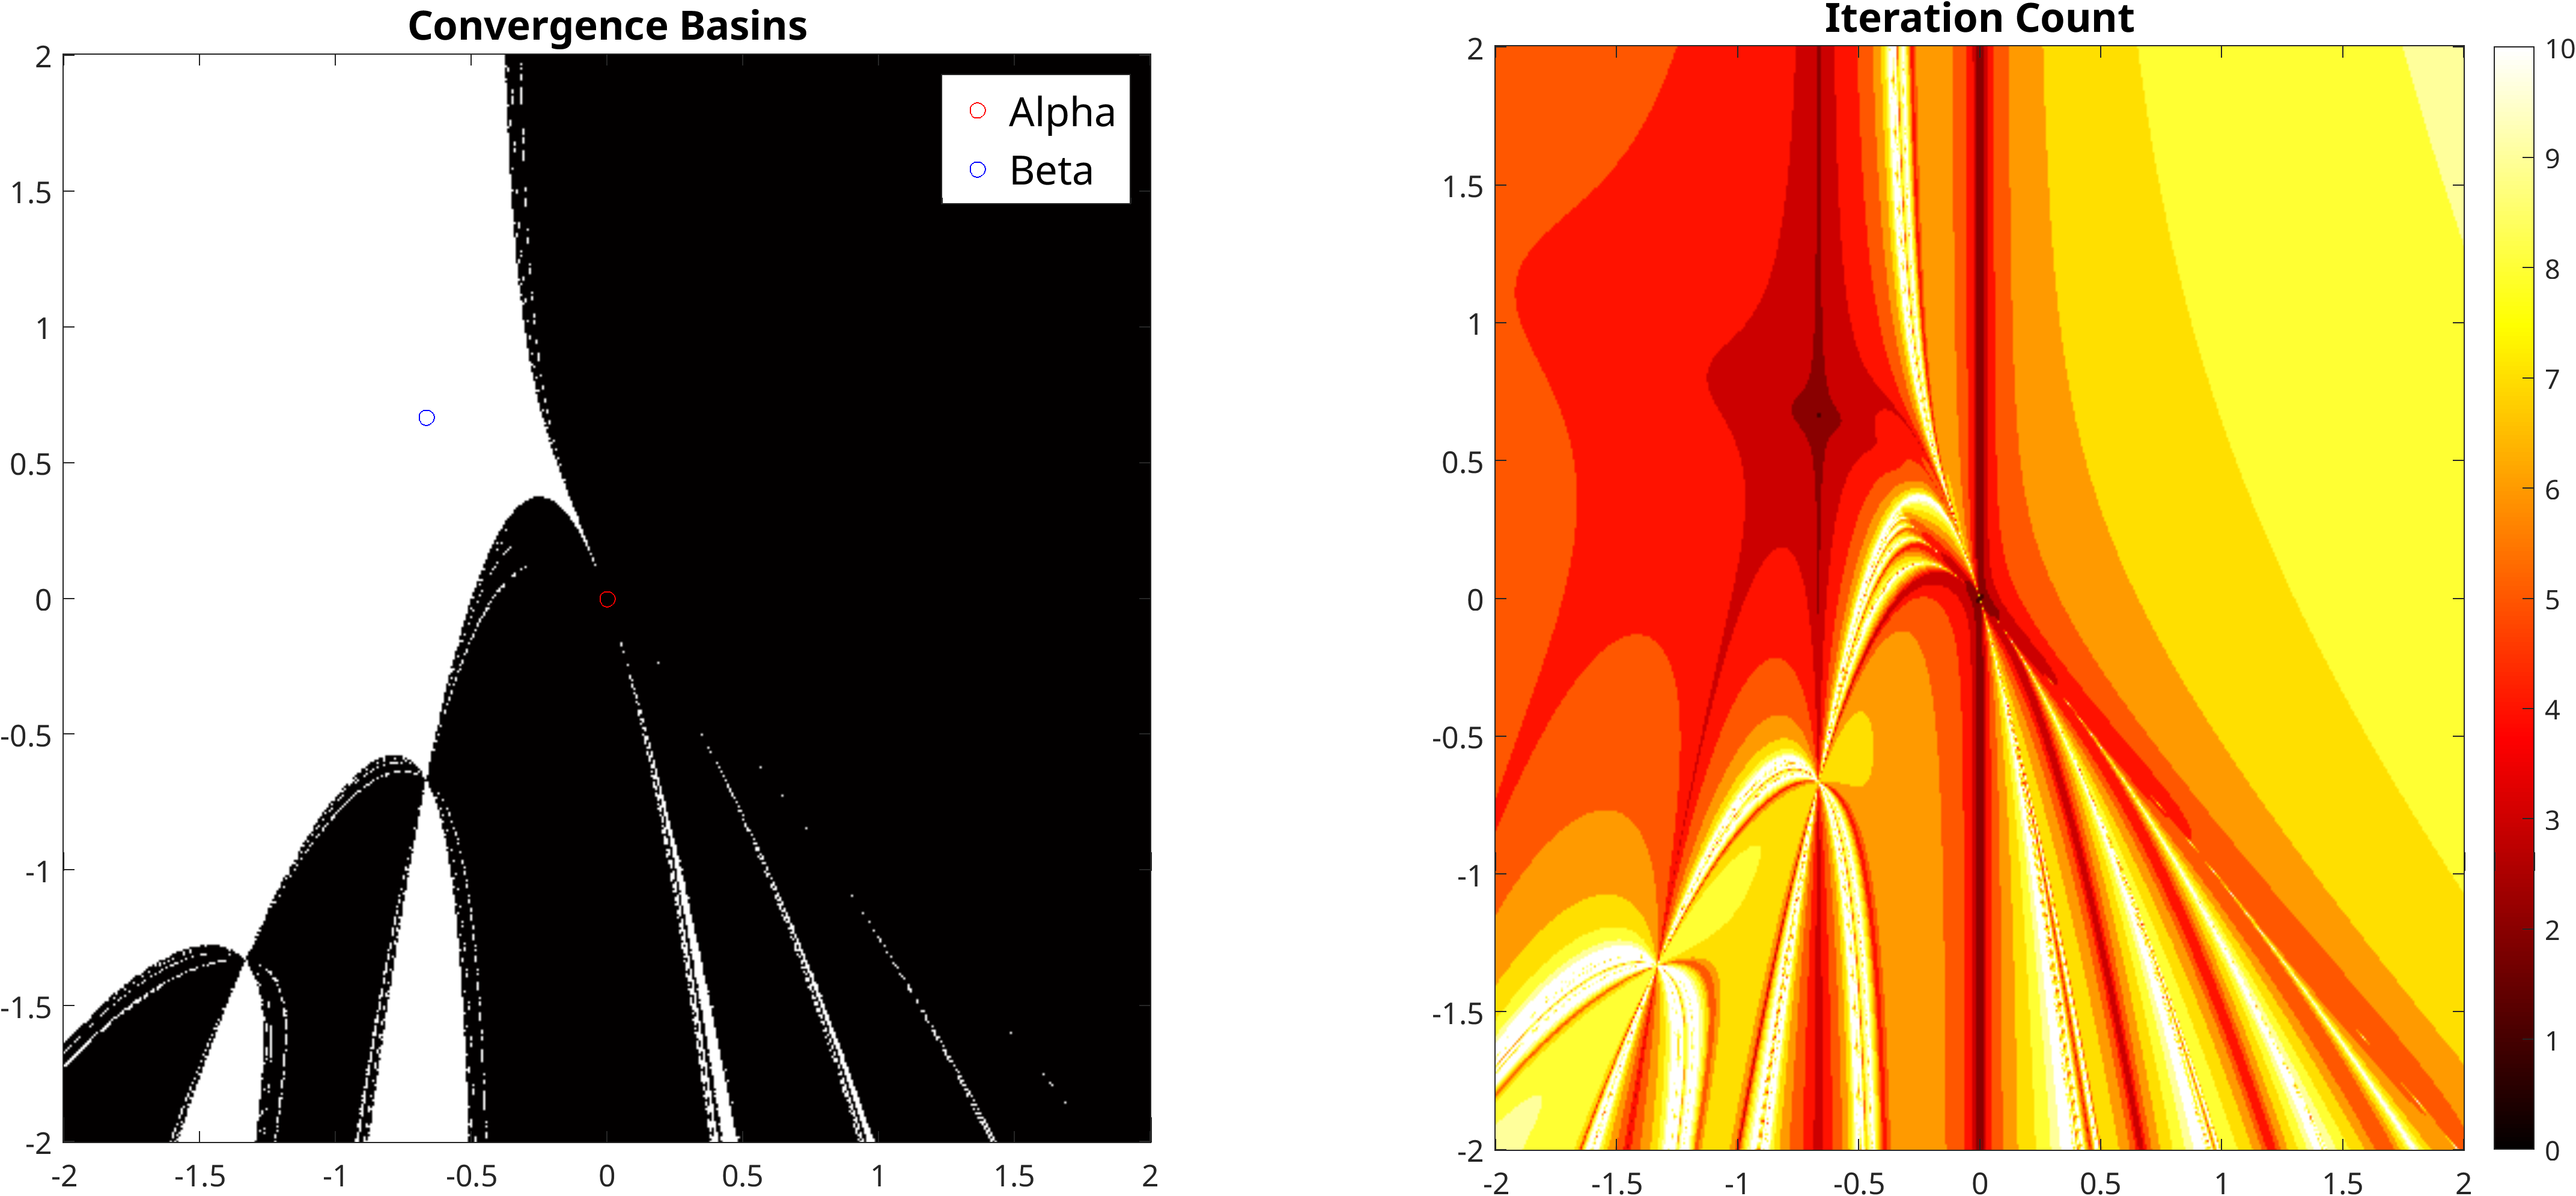
\includegraphics[scale=0.4]{../figures/raphson_conv.png}
\end{center}

Da dove si nota che la regione di convergenza in $\beta$ ha numeri di iterazione in media molto più piccoli rispetto alla regione di convergenza di $\alpha$.

Questo corrisponde con quanto avevamo trovato in maniera analitica, cioè che:
\begin{itemize}
	\item[$\alpha$]: $\det = 0$, e la convergenza non è superlineare;
	\item[$\beta$]: $\det \neq 0$, e la convergenza è superlineare;
\end{itemize}

\subsubsection{Varianti del metodo di Newton-Raphson}
Abbiamo che ad ogni passo del metodo di Newton-Raphson dobbiamo:
\begin{enumerate}
	\item Valutare $J_f(x^{(n)})$; ovvero $m^2$ funzioni non lineari;
	\item Risolvere $J_f(x^{(n)}) y = f(x^{(n)})$, sistema lineare $m \times m$ (complessità $O(m^3))$.
\end{enumerate}

Quando $m$ è particolarmente grande siamo disposti a fare qualcosa di più economico al prezzo di perdere l'ordine di convergenza molto favorevole di Newton-Rhapson.

\begin{enumerate}
	\item La prima strategia è quella di non aggiornare mai il Jacobiano (\textbf{Newton semplificato}).
		Il Jacobiano viene quindi calcolato solo in $x^{(0)}$ punto iniziale, e poi si usa sempre lo stesso nelle iterazioni successive, cioè l'aggiornamento diventa:
		$$
		x^{(n + 1)} = x^{(n)} - J_f(x^{(0)})^{-1} f(x^{(n)})
		$$
		
		Per la risoluzione del sistema, si può quindi sfruttare la fattorizzazione $LU$ del Jacobiano appena nominato, e quindi svolgere complessivamente due operazioni $O(m^2)$.

	\item La seconda strategia viene detta \textbf{metodo di Jacobi nonlineare}.
		Ad ogni passo si sostituisce $J_f(x^{(n)})$ con la matrice diagonale:
		$$
		\mathrm{diag} \left( \frac{\partial f}{\partial x_1} (x^{(n)}), ..., \frac{\partial f}{\partial x_m} (x^{(n)}) \right)
		$$
		così che:
		\begin{enumerate}
			\item Bisogna fare $m$ valutazioni di funzioni non lineari;
			\item Risolvere il sistema lineare costa $O(m)$.
		\end{enumerate}

		L'aggiornamento diventa quindi qualcosa del tipo:
		$$
		x_i^{(n + 1)} = x_i^{(n)} - \frac{f_i(x^{(n)})}{\frac{\partial f}{\partial x_i} (x_1^{(n)}, ..., x_m^{(n)})}
		$$

	\item La terza strategia viene detta \textbf{metodo di Gauss-Seidel nonlineare}.

		In questo caso l'aggiornamento è sostanzialmente analogo al metodo di Jacobi, con la differenza:
		$$
		x_i^{(n + 1)} = x_i^{(n)} - \frac{f_i(x_1^{(n + 1)}, ..., x_{i - 1}^{(n + 1)}, x_i^{(n)}, ... x_m^{(n)})}{\frac{\partial f}{\partial x_i} (x_1^{(n + 1)}, ..., x_{i - 1}^{(n + 1)}, x_i^{(n)}, ... x_m^{(n)})}
		$$
		dove le entrate $x^{(n + 1)}$ vengono calcolate una per volta attraverso le stesse considerazioni fatte per il metodo di Gauss-Seidel lineare.
\end{enumerate}

Altre varianti sono date dai cosiddetti metodi \textbf{quasi-Newton}, dove si sostituisce $J_f(x)$ con qualcosa con cui è più semplice (meno costoso) risolvere sistemi lineari e che richiedono meno valutazioni di funzioni non lineari.

\end{document}


\documentclass[a4paper,11pt]{article}
\usepackage[a4paper, margin=8em]{geometry}

% usa i pacchetti per la scrittura in italiano
\usepackage[french,italian]{babel}
\usepackage[T1]{fontenc}
\usepackage[utf8]{inputenc}
\frenchspacing 

% usa i pacchetti per la formattazione matematica
\usepackage{amsmath, amssymb, amsthm, amsfonts}

% usa altri pacchetti
\usepackage{gensymb}
\usepackage{hyperref}
\usepackage{standalone}

% imposta il titolo
\title{Appunti Calcolo Numerico}
\author{Luca Seggiani}
\date{2025}

% disegni
\usepackage{pgfplots}
\pgfplotsset{width=10cm,compat=1.9}

% imposta lo stile
% usa helvetica
\usepackage[scaled]{helvet}
% usa palatino
\usepackage{palatino}
% usa un font monospazio guardabile
\usepackage{lmodern}

% tikz in sans
\tikzset{every picture/.style={/utils/exec={\sffamily}}}

\renewcommand{\rmdefault}{ppl}
\renewcommand{\sfdefault}{phv}
\renewcommand{\ttdefault}{lmtt}

% circuiti
\usepackage{circuitikz}
\usetikzlibrary{babel}

% disponi il titolo
\makeatletter
\renewcommand{\maketitle} {
	\begin{center} 
		\begin{minipage}[t]{.8\textwidth}
			\textsf{\huge\bfseries \@title} 
		\end{minipage}%
		\begin{minipage}[t]{.2\textwidth}
			\raggedleft \vspace{-1.65em}
			\textsf{\small \@author} \vfill
			\textsf{\small \@date}
		\end{minipage}
		\par
	\end{center}

	\thispagestyle{empty}
	\pagestyle{fancy}
}
\makeatother

% disponi teoremi
\usepackage{tcolorbox}
\newtcolorbox[auto counter, number within=section]{theorem}[2][]{%
	colback=blue!10, 
	colframe=blue!40!black, 
	sharp corners=northwest,
	fonttitle=\sffamily\bfseries, 
	title=Teorema~\thetcbcounter: #2, 
	#1
}

% disponi definizioni
\newtcolorbox[auto counter, number within=section]{definition}[2][]{%
	colback=red!10,
	colframe=red!40!black,
	sharp corners=northwest,
	fonttitle=\sffamily\bfseries,
	title=Definizione~\thetcbcounter: #2,
	#1
}

% disponi problemi
\newtcolorbox[auto counter, number within=section]{problem}[2][]{%
	colback=green!10,
	colframe=green!40!black,
	sharp corners=northwest,
	fonttitle=\sffamily\bfseries,
	title=Problema~\thetcbcounter: #2,
	#1
}

% disponi codice
\usepackage{listings}
\usepackage[table]{xcolor}

\definecolor{codegreen}{rgb}{0,0.6,0}
\definecolor{codegray}{rgb}{0.5,0.5,0.5}
\definecolor{codepurple}{rgb}{0.58,0,0.82}
\definecolor{backcolour}{rgb}{0.95,0.95,0.92}

\lstdefinestyle{codestyle}{
		backgroundcolor=\color{black!5}, 
		commentstyle=\color{codegreen},
		keywordstyle=\bfseries\color{magenta},
		numberstyle=\sffamily\tiny\color{black!60},
		stringstyle=\color{green!50!black},
		basicstyle=\ttfamily\footnotesize,
		breakatwhitespace=false,         
		breaklines=true,                 
		captionpos=b,                    
		keepspaces=true,                 
		numbers=left,                    
		numbersep=5pt,                  
		showspaces=false,                
		showstringspaces=false,
		showtabs=false,                  
		tabsize=2
}

\lstdefinestyle{shellstyle}{
		backgroundcolor=\color{black!5}, 
		basicstyle=\ttfamily\footnotesize\color{black}, 
		commentstyle=\color{black}, 
		keywordstyle=\color{black},
		numberstyle=\color{black!5},
		stringstyle=\color{black}, 
		showspaces=false,
		showstringspaces=false, 
		showtabs=false, 
		tabsize=2, 
		numbers=none, 
		breaklines=true
}

\lstdefinelanguage{javascript}{
	keywords={typeof, new, true, false, catch, function, return, null, catch, switch, var, if, in, while, do, else, case, break},
	keywordstyle=\color{blue}\bfseries,
	ndkeywords={class, export, boolean, throw, implements, import, this},
	ndkeywordstyle=\color{darkgray}\bfseries,
	identifierstyle=\color{black},
	sensitive=false,
	comment=[l]{//},
	morecomment=[s]{/*}{*/},
	commentstyle=\color{purple}\ttfamily,
	stringstyle=\color{red}\ttfamily,
	morestring=[b]',
	morestring=[b]"
}

% disponi sezioni
\usepackage{titlesec}

\titleformat{\section}
	{\sffamily\Large\bfseries} 
	{\thesection}{1em}{} 
\titleformat{\subsection}
	{\sffamily\large\bfseries}   
	{\thesubsection}{1em}{} 
\titleformat{\subsubsection}
	{\sffamily\normalsize\bfseries} 
	{\thesubsubsection}{1em}{}

% disponi alberi
\usepackage{forest}

\forestset{
	rectstyle/.style={
		for tree={rectangle,draw,font=\large\sffamily}
	},
	roundstyle/.style={
		for tree={circle,draw,font=\large}
	}
}

% disponi algoritmi
\usepackage{algorithm}
\usepackage{algorithmic}
\makeatletter
\renewcommand{\ALG@name}{Algoritmo}
\makeatother

% disponi numeri di pagina
\usepackage{fancyhdr}
\fancyhf{} 
\fancyfoot[L]{\sffamily{\thepage}}

\makeatletter
\fancyhead[L]{\raisebox{1ex}[0pt][0pt]{\sffamily{\@title \ \@date}}} 
\fancyhead[R]{\raisebox{1ex}[0pt][0pt]{\sffamily{\@author}}}
\makeatother

\begin{document}

% sezione (data)
\section{Lezione del 19-05-25}

% stili pagina
\thispagestyle{empty}
\pagestyle{fancy}

% testo
\subsection{Calcolo di autovalori e autovettori}
Vediamo quindi il problema di, data una matrice $A \in \mathbb{C}^{n \times n}$, trovare auutocoppie $(\lambda, v)$, con $\lambda \in \mathbb{C}$, $v \in \mathbb{C}^n \setminus \{0\}$ che verificano:
$$
A v = \lambda v
$$

Vedremo 2 metodi iterativi che approcciano 2 versioni di questo problema:
\begin{enumerate}
	\item Calcolo di una singola autocoppia $(\lambda, v)$, ad esempio una coppia in cui $\lambda$ è l'autovalore di modulo massimo;
	\item Calcolo di tutte le autocoppie $(\lambda, v)$, ovvero una autocoppia per ogni autovalore distinto. Non approfondiremo questo metodo per questioni di complessità.
\end{enumerate}

Osserviamo che gli autovalori sono necessariamente $n$ contate le le loro molteplicità $\mu$, in quanto rappresentano le soluzioni di un polinomio di grado $n$, e altro non possono fare per via del teorema fondamentale dell'algebra.

Osserviamo poi che gli autovettori sono definiti a meno di moltiplicazione per scalare, cioè sono sempre infiniti gli autovettori associati ad un singolo autovalore $\lambda$ (tutti quelli nell'autopazio).

\subsubsection{Metodo delle potenze}
Vediamo il metodo 1) per ottenere una singola autocoppia, e in particolare quella di modulo (autovalore) massimo.
Questo può essere utile per:
\begin{itemize}
	\item Trovare il raggio spettrale di una matrice;
	\item Trovare la norma 2 di una matrice come:
		$$
			|A|_2 = \sqrt{\rho(A^H A)}
		$$
\end{itemize}

Supponiamo che $A$ sia diagonalizzabile.
Questa è l'ipotesi che ci assicura che ogni autovalore ha un autovettore associato linearmente indipendente.
Prendiamo quindi gli autovalori $\lambda_1, ..., \lambda_n$ posti che soddisfano:
$$
|\lambda_1| > |\lambda_2| \geq |\lambda_3| \geq ... \geq |\lambda_n|
$$
dove il primo è in maggiorazione stretta (altrimenti non si distinguerebbe un unico autovalore di modulo massimo).

Dato che $A$ è diagonalizzabile, abbiamo dai fondamenti di algebra lineare che esiste una base di $\mathbb{C}^n$ fatta da autovettori di $A$, ovvero $\exists v^{(1)}, ..., v^{(n)} \in \mathbb{C}^n$ tali che:
$$
A v^{(j)} = \lambda_j v^{(j)}, \quad j = 1, ..., n
$$
e per ogni $z \in \mathbb{C}^n$ vale che $\exists ! c_1, .., c_n \in \mathbb{C}$ tali che:
$$
z = \sum_{j = 1}^n c_j v^{(j)} = c_1 v^{(1)} + ... c_n v^{(n)}
$$

\par\smallskip

L'idea fondamentale del metodo è che, preso $z \in \mathbb{C}^n$ a caso, abbiamo:
$$
A z = A (c_1 v^{(1)} + ... + c_n v^{(n)}) = c_1 A v^{(1)} + ... + c_n A v^{(n)} = c_1 \lambda_1 v^{(1)} + ... + c_n \lambda_n v^{(n)}
$$
Continuando ad iterare si ha:
$$
A^2 z = A (Az) = A (c_1 \lambda_1 v^{(1)} + ... + c_n \lambda_n v^{(n)})
$$
$$
= c_1 \lambda_1 A v^{(1)} + ... + c_n \lambda_b A v^{(n)} = c_1 \lambda_1^2 v^{(1)} + ... + c_n \lambda_n^2 v^{(n)}
$$
e quindi continuando ad iterare si ha che:
$$
A^k z = c_1 \lambda_1^k v^{(1)} + ... + c_n \lambda_n^k v^{(n)}
$$

Il vantaggio è che l'autovalore di modulo massimo compare chiaramente con contribuzioni sempre più grandi, in quanto:
$$
= \lambda_1^k \left( c_1 v^{(1)} + c_2 \left( \frac{\lambda_2}{\lambda_1} \right)^k v^{(2)} + ... + c_n \left( \frac{\lambda_n}{\lambda_1} \right)^k v^{(n)} \right) \sim \lambda_1^k, \quad k \rightarrow + \infty
$$

Più formalmente, abbiamo che vale il teorema:
\begin{theorem}{Convergenza del metodo delle potenze}
	Sia considerata la successione:
	\[
		\begin{cases}
			z^{(0)} = z \\
			z^{(k + 1)} = Az^{(k)} = A^{k + 1} z^{(0)} = A^{k + 1} z
		\end{cases}
	\]
	con $A \in \mathbb{C}^{n \times n}$ hermitiana ($A = A^H$), con autovalori:
	$$
	|\lambda_1| > |\lambda_2| \geq |\lambda_3| \geq ... \geq |\lambda_n| > 0
	$$
	e sia $h \in \{1, ..., n\}$ tale per cui $v_h^{(1)} \neq 0$.
	Se $z^{(0)} \in \mathbb{C}^n$ è tale che:
	$$
	\left[V^{(1)}\right]^H z^{(0)} \neq 0
	$$
	allora la successione è tale che:
	$$
	\lim_{k \rightarrow +\infty} \frac{z^{(k)}}{z_h^{(k)}} = \tilde{v}^{(1)}
	$$
	multiplo scalare di $v^{(1)}$ (in particolare $\tilde{v}^{(1)} = \frac{v^{(1)}}{v_h^{(1)}}$).
	Inoltre, per l'autovalore vale:
	$$
	\lim_{k \rightarrow +\infty} \frac{\left[ z^{(k)} \right]^H A z^{(k)}}{\left[ z^{(k)} \right]^H z^{(k)}} = \lambda_1
	$$
\end{theorem}

Osserviamo che, dato $x \in \mathbb{C}^n$ e considerato il \textit{quoziente di Rayleigh}:
$$
R(x) = \frac{x^H A x}{x^H x}
$$
Se $x$ verifica $Ax = \lambda x$ (cioè è autovettore) allora:
$$
R(x) = \frac{x^H A x}{x^H x} = \frac{x^H \lambda x}{x^H x} = \lambda \frac{x^H x}{x^H x} = \lambda
$$

Notiamo la motivazione dell'assunto di matrice hermitiana.
Di base, per il teorema spettrale si ha che:
$$
A = A^H \implies A \text{ diagonalizzabile}
$$
e in particolare si può scegliere una base ortonormale di autovettori, cioè trovare $v^{(1)}, ..., v^{(n)} \in \mathbb{C}^n$ tali che:
$$
A v^{(j)} = \lambda_j v^{(j)}, \quad \left[ v^{(i)} \right]^H v^{(j)} = \, < v^{(i)}, v^{(j)} > \, =
	\begin{cases}
		0, \quad i \neq j \\
		1, \quad i = j
	\end{cases}
$$
cioè equivalentemente:
$$
A = V D V^H
$$
con $D$ diagonalizzabile e $V$ normale data dagli autovettori in colonna.

\par\smallskip

Dimostriamo quindi il teorema.
Dato che $A = A^H$ hermitiana si ha che:
$$
z^{(0)} = \sum_{j = 1}^n c_j v^{(j)} 
$$
ed inoltre abbiamo:
$$
0 \neq \left[ v^{(1)} \right]^H z^{(0)} = \sum_{j = 1}^n c_j \left[ v^{(1)} \right]^H v^{(j)} = c_1 \left[ v^{(1)} \right]^H v^{(1)} = c_1
$$
e quindi $c_1 \neq 0$.

Dimostriamo allora le due tesi, su autovettore (1) a autovalore massimo (2):
\begin{enumerate}
	\item 
Come fatto in precedenza prendiamo: 
$$
z^{(k)} = A^k z^{(0)} = \lambda_1^k \left( c_1 v^{(1)} + c_2 \left( \frac{\lambda_2}{\lambda_1} \right)^k v^{(2)} + ... + c_n \left( \frac{\lambda_n}{\lambda_1} \right)^k v^{(n)} \right)
$$
$$
= \lambda_1^k \left( c_1 v^{(1)} + \sum_{j = 2}^n \left(\frac{\lambda_j}{\lambda_i}\right)^k v^{(j)} c_j \right)
$$
dove vorremo dimostrare che il termine a destra scompare per $k \rightarrow +\infty$.

Prendiamo quindi il limite:
$$
\lim_{k \rightarrow +\infty} \frac{ \lambda_1^k \left( c_1 v^{(1)} + \sum_{j = 2}^n \left(\frac{\lambda_j}{\lambda_i}\right)^k v^{(j)} c_j \right) }{ \lambda_1^k \left( c_1 v^{(1)}_h + \sum_{j = 2}^n \left(\frac{\lambda_j}{\lambda_i}\right)^k v^{(j)}_h c_j \right) }
$$
$$
\lim_{k \rightarrow +\infty} \frac{ c_1 v^{(1)} + \sum_{j = 2}^n \left(\frac{\lambda_j}{\lambda_i}\right)^k v^{(j)} c_j ) }{ c_1 v^{(1)}_h + \sum_{j = 2}^n \left(\frac{\lambda_j}{\lambda_i}\right)^k v^{(j)}_h c_j }
= \lim_{n \rightarrow + \infty} \frac{c_1 v^{(1)}}{c_1 v_h^{(1)}} = \frac{v^{(1)}}{v_h^{1}}
$$
che è la prima tesi.

	\item
Prendiamo quindi:
$$
\lim_{k \rightarrow + \infty} \frac{\left[ z^{(k)} \right]^H A z^{(k)}}{\left[ z^{(k)} \right]^H z^{(k)}} 
= \lim_{k \rightarrow + \infty} \frac{ \left[ \frac{z^{(k)}}{z_h^{(k)}} \right]^H A \frac{z^{(k)}}{z_h^{(k)}} }{ \left[ \frac{z^{(k)}}{z^{(k)}_h} \right]^H A \frac{z^{(k)}}{z^{(k)}_h} }
= \frac{ \left[ \frac{v^{(1)}}{v_h^{(1)}} \right]^H A \frac{v^{(1)}}{v_h^{(1)}} }{ \left[ \frac{v^{(1)}}{v^{(1)}_h} \right]^H A \frac{v^{(1)}}{v^{(1)}_h} } 
$$
che moltiplicando sopra e sotto per $\left( v_h^{(1)} \right)^2$ dà:
$$
= \frac{ [v^{(1)} ]^H A v^{(1)} }{ [v^{(1)}]^H v^{(1)} } = \lambda_1
$$
da cui la seconda tesi. \qed
\end{enumerate}

Osserviamo che $h$ è stato usato perché dividiamo per $z_h^{(k)}$ che per $k$ abbastnza grandi è $\neq 0$, in quanto vicino a $v_h^{(1)}$.

Osserviamo poi che nell'implementazione pratica il metodo delle potenze $z^{(k)}$ viene diviso per la sua norma, così da ottenere solo vettori di norma $1$ ed evitare problemi di overflow o underflow.

Potremmo infatti avere, ad esempio, dello pseudocodice di esempio:
\begin{lstlisting}[language=MATLAB, style=codestyle]	
input z[0]

for k = 1, 2, 3, ...
	y[k] = A * z[k - 1]
	z[k] = y[k] / ( |y[k]|_2 )
end
\end{lstlisting}

Il costo è quello di una nomrma ($O(n)$) e di un prodotto matrice vettore ($O(n^2)$ )ad ogni iterazione, cioè $O(k \cdot n^2)$.

\subsubsection{Criterio di stop}
Vediamo la condizione di stop del metodo delle potenze.
In genere si usa:
$$
|R(z^{(k)} - R(z^{(k - 1)}))| < \epsilon
$$
con ad esempio $\epsilon = 10^{-8}$.

Testiamo gli autovalori con $R()$ e non gli autovettori con:
$$
|z^{(k)} - z^{(k + 1)}|_2 < \epsilon
$$
in quanto non sappiamo verso quale multiplo scalare degli autovettori ci stiamo dirigendo, per cui la differenza ad ogni passaggio potrebbe essere molto grande.

\subsubsection{Commenti sull'ipotesi di convergenza}
Possiamo fare un commento sulle ipotesi del teorema 22.1.
\begin{itemize}
	\item Non è strettamente necessario che $A = A^H$ hermitiana, in quanto si può dimostrare che il metodo funziona anche con $A$ solo diagonalizzabile;
	\item L'assunzione $\left[ v^{(1)} \right]^H z^{(0)} \neq 0$ è virtualmente vera (o meglio vera con probabilità $1$) per qualsiasi $z^{(0)} \in \mathbb{C}^n$ scelto a caso.
		Inoltre, nel caso di calcolo a macchina si ha che gli errori di arrotondamento stessi aiutano ad uscire dall'ortogonalità, anche se si parte da tale condizione.
		\item L'assunzione $|\lambda_1| > |\lambda_2|$ non è invece rinunciabile, in quanto si possono costruire esempi di successioni non convergenti nel caso di più autovalori dominanti.

			Prendiamo l'esempio:
			$$
				A =
				\begin{pmatrix}
					0 & 1 \\ 
					1 & 0
				\end{pmatrix}
			$$
			con 2 autovalori di modulo 1.
			Prendiamo:
			$$
			z^{(0)} = 
			\begin{pmatrix}
				2 \\ 3
			\end{pmatrix}
			$$
			Si trova che l'aggiornamento scambia semplicemente le componenti:
			$$
			A z^{(0)} =
			\begin{pmatrix}
				3 \\ 2
			\end{pmatrix}
			$$
			e cosi via all'infinito.

			Gli autovettori, calcolati a mano, sono semplicemente:
			$$
				v^{(1)} =
				\begin{pmatrix}
					1 \\ 1
				\end{pmatrix}, \quad
				v^{(2)} =
				\begin{pmatrix}
					1 \\ -1
				\end{pmatrix}
			$$
\end{itemize}

Osserviamo quindi che per eseguire il metodo delle potenze, serve soltanto essere in grado di valutare il prodotto matrice vettore $A z$.
Questo può essere utile nel caso sopra citato, quando si ha una matrice definita come risultato di operazioni aritmetiche, magari costose.

Ad esempio, se si vuole stimare:
$$
|A|_2 = \sqrt{\rho(A^H A)}
$$
si può pensare di applicare il metodo delle potenze su $A^H A$, senza nemmeno dover calcolare $A^H A$ ma applicando direttamente i prodotti matrici vettore $A^H A z$.

\subsection{Metodi per più autovalori}
\subsubsection{Autovalori minimi}
Supponiamo di essere interessati all'autocoppia $(\lambda_n, v^{(n)})$, associata all'autovalore $\lambda_n$ di modulo minimo, e supponiamo:
$$
|\lambda_1| \geq ... \geq |\lambda_{n - 2}| \geq |\lambda_{n - 1}| > |\lambda_n|
$$

L'idea è di applicare il metodo delle potenze ad $A^{-1}$, infatti $A^{-1}$ ha autovalori:
$$
\left| \frac{1}{\lambda_n} \right| > \left| \frac{1}{\lambda_{n - 1}} \right| \geq \left| \frac{1}{\lambda_{n - 2}} \right| \geq ... \geq \left| \frac{1}{\lambda_1} \right|
$$
ed inoltre ha come autovettori $v^{(1)}, ..., v^{(n)}$.
Quidi le successioni generate dal metodo delle potenze su $A^{-1}$ convergono all'autocoppia:
$$
\left( \frac{1}{\lambda_n}, v^{(n)} \right)
$$

Chiamiamo questo metodo anche \textbf{metodo delle potenze inverse}, che implementiamo in pseudocodice come:
\begin{lstlisting}[language=MATLAB, style=codestyle]	
input z[0]

for k = 1, 2, 3, ...
	y[k] = inv(A) * z[k - 1]
	z[k] = y[k] / ( |y[k]|_2 )
end

% qui manca il quoziente di Rayleigh perche' z e' gia normalizzato 
l_n = 1 / ( (z[K])^H A z[K] )
\end{lstlisting}

Dove chiaramente non vale la pena di calcolare l'inversa ma piuttosto conviene risolvere il sistema:
$$
A y^{(k)} = z^{(k - 1)}
$$
ad esempio sfruttando l'eliminazione di Gauss con pivoting.
Per rendere tutto più efficiente, conviene anzi precalcolare una fattorizzazione $LU$ di $A$ prima di iniziare il metodo.

In questo caso avremo:
$$
A = \Pi LU
$$
cioè si fa una fattorizzazione $LU$ con pivoting dato dalla matrice di permutazione $\Pi$, così che ad ogni passaggio il prodotto $A^{-1} z$ diventa equivalente a risolvere un sistema lineare triangolare.
In questo caso il costo diventa $O(n^3)$ per la fattorizzazione più $O(k \cdot n^2)$ per la risoluzione dei sistemi triangolari.

\subsubsection{Autovalori intermedi}
Vediamo quindi come modificare il metodo delle potenze per trovare un autovalore intermedio, cioè preso $\sigma \in \mathbb{C}$ scalare arbitrario calcolare l'autocoppia $(\lambda, v)$ con $\lambda$ più vicino a $\sigma$.

In questo caso si applica il metodo delle potenze alla matrice:
$$
A \sim (A - \sigma \cdot I)^{-1}
$$
che ha gli stessi autovettori di $A$ e come autovalori ha quantità della forma:
$$
\lambda_j' = \frac{1}{\lambda_j - \sigma}
$$
In questo caso l'autovalore di modulo più grande diventa quello più vicino a $\sigma$, per cui basta applicare il metodo delle potenze.


\end{document}


\documentclass[a4paper,11pt]{article}
\usepackage[a4paper, margin=8em]{geometry}

% usa i pacchetti per la scrittura in italiano
\usepackage[french,italian]{babel}
\usepackage[T1]{fontenc}
\usepackage[utf8]{inputenc}
\frenchspacing 

% usa i pacchetti per la formattazione matematica
\usepackage{amsmath, amssymb, amsthm, amsfonts}

% usa altri pacchetti
\usepackage{gensymb}
\usepackage{hyperref}
\usepackage{standalone}

% imposta il titolo
\title{Appunti Calcolo Numerico}
\author{Luca Seggiani}
\date{2025}

% disegni
\usepackage{pgfplots}
\pgfplotsset{width=10cm,compat=1.9}

% imposta lo stile
% usa helvetica
\usepackage[scaled]{helvet}
% usa palatino
\usepackage{palatino}
% usa un font monospazio guardabile
\usepackage{lmodern}

% tikz in sans
\tikzset{every picture/.style={/utils/exec={\sffamily}}}

\renewcommand{\rmdefault}{ppl}
\renewcommand{\sfdefault}{phv}
\renewcommand{\ttdefault}{lmtt}

% circuiti
\usepackage{circuitikz}
\usetikzlibrary{babel}

% disponi il titolo
\makeatletter
\renewcommand{\maketitle} {
	\begin{center} 
		\begin{minipage}[t]{.8\textwidth}
			\textsf{\huge\bfseries \@title} 
		\end{minipage}%
		\begin{minipage}[t]{.2\textwidth}
			\raggedleft \vspace{-1.65em}
			\textsf{\small \@author} \vfill
			\textsf{\small \@date}
		\end{minipage}
		\par
	\end{center}

	\thispagestyle{empty}
	\pagestyle{fancy}
}
\makeatother

% disponi teoremi
\usepackage{tcolorbox}
\newtcolorbox[auto counter, number within=section]{theorem}[2][]{%
	colback=blue!10, 
	colframe=blue!40!black, 
	sharp corners=northwest,
	fonttitle=\sffamily\bfseries, 
	title=Teorema~\thetcbcounter: #2, 
	#1
}

% disponi definizioni
\newtcolorbox[auto counter, number within=section]{definition}[2][]{%
	colback=red!10,
	colframe=red!40!black,
	sharp corners=northwest,
	fonttitle=\sffamily\bfseries,
	title=Definizione~\thetcbcounter: #2,
	#1
}

% disponi problemi
\newtcolorbox[auto counter, number within=section]{problem}[2][]{%
	colback=green!10,
	colframe=green!40!black,
	sharp corners=northwest,
	fonttitle=\sffamily\bfseries,
	title=Problema~\thetcbcounter: #2,
	#1
}

% disponi codice
\usepackage{listings}
\usepackage[table]{xcolor}

\definecolor{codegreen}{rgb}{0,0.6,0}
\definecolor{codegray}{rgb}{0.5,0.5,0.5}
\definecolor{codepurple}{rgb}{0.58,0,0.82}
\definecolor{backcolour}{rgb}{0.95,0.95,0.92}

\lstdefinestyle{codestyle}{
		backgroundcolor=\color{black!5}, 
		commentstyle=\color{codegreen},
		keywordstyle=\bfseries\color{magenta},
		numberstyle=\sffamily\tiny\color{black!60},
		stringstyle=\color{green!50!black},
		basicstyle=\ttfamily\footnotesize,
		breakatwhitespace=false,         
		breaklines=true,                 
		captionpos=b,                    
		keepspaces=true,                 
		numbers=left,                    
		numbersep=5pt,                  
		showspaces=false,                
		showstringspaces=false,
		showtabs=false,                  
		tabsize=2
}

\lstdefinestyle{shellstyle}{
		backgroundcolor=\color{black!5}, 
		basicstyle=\ttfamily\footnotesize\color{black}, 
		commentstyle=\color{black}, 
		keywordstyle=\color{black},
		numberstyle=\color{black!5},
		stringstyle=\color{black}, 
		showspaces=false,
		showstringspaces=false, 
		showtabs=false, 
		tabsize=2, 
		numbers=none, 
		breaklines=true
}

\lstdefinelanguage{javascript}{
	keywords={typeof, new, true, false, catch, function, return, null, catch, switch, var, if, in, while, do, else, case, break},
	keywordstyle=\color{blue}\bfseries,
	ndkeywords={class, export, boolean, throw, implements, import, this},
	ndkeywordstyle=\color{darkgray}\bfseries,
	identifierstyle=\color{black},
	sensitive=false,
	comment=[l]{//},
	morecomment=[s]{/*}{*/},
	commentstyle=\color{purple}\ttfamily,
	stringstyle=\color{red}\ttfamily,
	morestring=[b]',
	morestring=[b]"
}

% disponi sezioni
\usepackage{titlesec}

\titleformat{\section}
	{\sffamily\Large\bfseries} 
	{\thesection}{1em}{} 
\titleformat{\subsection}
	{\sffamily\large\bfseries}   
	{\thesubsection}{1em}{} 
\titleformat{\subsubsection}
	{\sffamily\normalsize\bfseries} 
	{\thesubsubsection}{1em}{}

% disponi alberi
\usepackage{forest}

\forestset{
	rectstyle/.style={
		for tree={rectangle,draw,font=\large\sffamily}
	},
	roundstyle/.style={
		for tree={circle,draw,font=\large}
	}
}

% disponi algoritmi
\usepackage{algorithm}
\usepackage{algorithmic}
\makeatletter
\renewcommand{\ALG@name}{Algoritmo}
\makeatother

% disponi numeri di pagina
\usepackage{fancyhdr}
\fancyhf{} 
\fancyfoot[L]{\sffamily{\thepage}}

\makeatletter
\fancyhead[L]{\raisebox{1ex}[0pt][0pt]{\sffamily{\@title \ \@date}}} 
\fancyhead[R]{\raisebox{1ex}[0pt][0pt]{\sffamily{\@author}}}
\makeatother

\begin{document}

% sezione (data)
\section{Lezione del 23-05-25}
% stili pagina
\thispagestyle{empty}
\pagestyle{fancy}

% testo
Continuiamo a vedere i metodi per più autovalori.

\subsubsection{Metodo QR per gli autovalori}
Introduciamo quindi il \textbf{metodo QR per gli autovalori}, che non va confuso col metodo QR \textit{per i minimi quadrati} (visto in 12.2), anche se chiaramente si basa sulla fattorizzazione QR.

Questo è quindi un metodo per trovare tutti gli autovalori di $A \in \mathbb{C}^{n \times n}$ e un insieme di autovettori associati a ciascun autovalore.
Abbiamo quindi come input $A$, de come uscita $V$ e $D$, con $D$ diagonale di autovalori:
$$
D =
\begin{pmatrix}
	\lambda_1 & ... & 0 \\
						& \ddots & \\
	0 & ... & \lambda_n
\end{pmatrix}
$$
e $V$ tale che:
$$
A = V D V^{-1}
$$

L'algoritmo che risolve questo problema viene ideato negli anni '70, ed è considerato fra i più importanti degli ultimi anni.
Vedremo una versione \textit{"vanilla"}, quindi semplificata, dell'algoritmo, in quanto le implementazioni moderne (MATLAB o librerie come \textit{LAPACK})non sarebbero effettivamente utili se non per le ottimizzazioni che sono state fatte nel tempo.

L'idea di fondo è creare una successione di matrici:
$$ \{A_k\}_{k \in \mathbb{N}}, \quad A_0 = A$$
tutte simili ad $A$, cioè tali che:
$$
\forall k, \ \exists Q \ : \ Q^{-1} A_k Q = A
$$
con $Q$ invertibile ed unitaria, cioè:
$$
Q^{-1} = Q^H
$$
In questo modo ogni $A_k$ ha gli stessi autovalori di $A$, mentre gli autovettori di $A_K = Q^H A Q$ saranno $Q^h v$, dove $v$ è autovettore di $A$.
Inoltre, chiamando:
$$
A_{\infty} = \lim_{k \rightarrow +\infty} A_k
$$
si ha che $A_{\infty}$ è unna matrice di cui si possono calcolare gli autovettori e autovalori in modo efficiente.
Nello specifico, $A_{\infty}$ è una matrice triangolare.

\subsubsection{Calcolo di autovalori e autovettori per matrici triangolari}
Motiviamo quindi quest'ultima affermazione studiando il caso particolare delle matrici triangolari. 
Poniamo $T$ triangolare superiore:
$$
T = 
\begin{pmatrix}
	t_{11} & ... & t_{1n} \\ 
				 & \ddots & \vdots \\
	0 & & t_{nn}
\end{pmatrix}
$$
gli autovalori sono facili, in quanto risulteranno:
$$
\{ t_{11}, t_{22}, ..., t_{nn} \}
$$
gli autovettori sono più difficili, ma vediamo che il primo è banale:
$$
T v_1 = \begin{pmatrix}
	t_{11} \\ 0 \\ \vdots \\ 0
\end{pmatrix}
=
t_{11}
\begin{pmatrix}
	1 \\ 0 \\ \vdots \\ 0
\end{pmatrix}
\implies
v_1 = 
\begin{pmatrix}
	1 \\ 0 \\ \vdots \\ 0
\end{pmatrix}
$$

Cerchiamo quini il generico autovettore $v_j$ assumedo $t_{ii} \neq t_{jj}$, $\forall i \neq j$ (cioè l'ipotesi degli autovalori distinti) e cerchiamo una soluzione diversa da 0 del sistema:
$$
(T - t_{jj} I) v_j = 0
$$
che avrà l'aspetto:
$$
\begin{pmatrix}
	t_{11} - t_{jj} & t_{12} & ... & & & &  t_{1n} \\ 
									& \ddots & ... & & & &  \vdots \\
									& & t_{j-1,j-1} - t_{jj} & ... & & &  \vdots \\
									& & & 0 & ... &  &  \vdots \\
									& & & & t_{j+1,j+1} - t_{jj} & ... &  \vdots \\
									& & & & & \ddots &  \vdots \\
									& & & & & & t_{nn} - t_{jj}
\end{pmatrix}
v_j = 
\begin{pmatrix}
	0 \\ \vdots \\ \vdots \\ \vdots \\ \vdots \\ \vdots \\ 0
\end{pmatrix}
$$

Riscrivendo a blocchi abbiamo:
$$
\begin{pmatrix}
	(T_1) & z & (*) \\ 
				& 0 & (*)  \\ 
				& & (T_2)
\end{pmatrix}
\underbrace{
\begin{pmatrix}
	(v_j^{(1)}) \\ \gamma \\ v_{j}^{(2)} 
\end{pmatrix}
}_{v_j}
=
\begin{pmatrix}
	0 \\ \vdots \\ 0
\end{pmatrix}
\, \Leftrightarrow \,
\begin{cases}
	T_1 v_j^{(1)} + \gamma z + (*) v_j^{(2)} = 0 \\ 
	... \\ 
	T_2 v_j^{(2)} = 0
\end{cases}
$$

Notiamo che:
$$
T_2 v_j^{(2)} = 0
$$
è un sistema $(n - j - 1) \times (n - j - 1)$ ha matrice invertibile, per cui:
$$
v_j^{(2)} = 0
$$
e la parte indicata con asterischi del sistema non ci interessa, per cui possiamo dire:
$$
T_1 v_j^{(1)} + \gamma z = 0
$$
che è un sistema $(j - 1) \times j$, cioè sottodeterminato.
Scegliamo ad esempio $\gamma = 1$ per fissare una soluzione, e otteniamo:
$$
T_1 v_j^{(1)} = -z \implies v_j^{(1)} = - T_1^{-1} z
$$
Per cui abbiamo ricostruito l'intero vettore $v_j$ come:
$$
v_j =
\begin{pmatrix}
	-T_1^{-1} z \\ 
	1 \\ 
	0 \\
	\vdots \\ 
	0
\end{pmatrix}
$$
Iteriamo quindi per gli $j = 1, ..., n$ indici e troviamo tutti gli autovettori.

Dal punto di vista del costo, per trovare $v_j $ si deve risolvere il sistema $T_1 x = -z$ di dimensione $(j - 1) \times (j - 1)$ e triangolare, che costa $O(j^2)$.
Col fatto che iteriamo per $j$ volte abbiamo complessivamente:
$$
O\left( \sum_{j = 1}^n j^2 \right) = O(n^3)
$$

\subsubsection{Metodo QR per la successione}
Vediamo quindi come formare la successione vera e propria.
L'idea è che prendiamo $A_0 = A$, e per $k = 1, 2, ...$ prendiamo:
$$
A_{k - 1} = Q_{k - 1} R_{k - 1}
$$
$$
A_k = R_{k - 1} Q_{k - 1}
$$

In effetti le matrici $A_k$ sono simili:
$$
A_{k + 1} = R_k Q_k = Q_k^H Q_k R_k Q_k = Q_k^H A_k Q_k
$$
espandendo $R_k$, e quindi $A_{k + 1}$ è simile ad $A_k$.
Iterando il ragionamento si ottiene che $A_{k + 1}$ è simile ad $A_0$ e quindi ad $A$.

In particolare:
$$
A_{k + 1} = Q_k^H A_k Q_k = Q_k^H Q_{k - 1}^H A_{k - 1} Q_{k - 1} Q_k
= ... = \underbrace{ Q_k^H Q_{k - 1}^H ... Q_1^H }_{\tilde{Q}_k^H} A \underbrace{ Q_1 ... Q_{k - 1} Q_k }_{\tilde{Q}_k}
$$
e quindi:
$$
A_{k + 1} = \tilde{Q}_k^H A \tilde{Q}_k
$$
da cui immediatamente la similarità con $\tilde{Q}_k$ matrice di traduzinoe.

A giustificare questo abbiamo il teorema:
\begin{theorem}{Validità del metodo QR agli autovalori}
	Presa $A \in \mathbb{R}^{n \times n}$ e supposto:
	$$
	|\lambda_1| > |\lambda_2| > ... > |\lambda_n|
	$$
	allora:
	$$
	\lim_{n \rightarrow +\infty} A_k = T = 
\begin{pmatrix}
	t_{11} & ... & t_{1n} \\ 
				 & \ddots & \vdots \\
	0 & & t_{nn}
\end{pmatrix}
	$$
	dove i blocchi $T_{jj}$ sono $1 \times 1$ per autovalori reali e $2 \times 2$ per autovalori complessi coniugati.
\end{theorem}

\subsubsection{Implementazione MATLAB del metodo QR per gli autovalori}
Vediamo quindi l'implementazione MATLAB della versione semplificata del metodo che abbiamo visto.
Innanzitutto ci dotiamo di una funzione per il calcolo delle autocoppie di matrici triangolari superiori $T$ come abbiamo visto in 23.0.2:
\begin{lstlisting}[language=MATLAB, style=codestyle]	
function [V, D] = eigu(T)
		n = height(T);

		D = diag(diag(T));

		V = zeros(n);
		
		for j = 1:n
				Tu = T(1:j - 1, 1:j - 1) - T(j, j) * eye(j - 1);
				z = T(1:j - 1, j);
				Viu = - (Tu \ z);
				
				V(1:j - 1, j) = Viu;
				V(j, j) = 1;
		end
end
\end{lstlisting}
che includeremo come sottofunzione.
A questo punto basterà implementare il passo iterativo:
\lstset{style=codestyle, language=MATLAB}
\lstinputlisting{../code/matlab/qr_eigen.m}

\subsubsection{Precisazioni sul metodo QR per gli autovalori}
Vediamo che i termini sotto a cui abbiamo definito l'algoritmo sono estremamente restrittivi (autovalori distinti, ecc...).
Chiaramente nelle implementazioni reali ci sono, oltre che alle ottimizzazioni, vari accorgimenti che rendono l'algoritmo robusto alle varie casistiche (autovalori ripetuti, ecc...), mantenendo il costo cubico $O(n^3)$.

Alcuni accorgimenti sono:
\begin{enumerate}
	\item Si deve tenere il numero di iterazioni $N$ sotto controllo, e in particolare viene garantito che:
		$$
		N = O(n)
		$$
	\item Calcolare la fattorizzazione QR costa $O(n^3)$, se la calcoliamo ad ogni passo ottieniamo un costo $O(n^4)$ che non è ottimale.
		Nella versione finale si fa un preprocessing sulla matrice $A$ che la riduce alla cosiddetta \textit{forma di Hessenberg} che rende il costo del calcolo della fattorizzazione quadratico $O(n^2)$ anziché cubico, così che l'algoritmo complessivo costi $O(n^3)$;
	\item Nella soluzione che abbiamo visto si fanno assunzioni sugli autovalori (autovettori distinti, moduli distinti, ecc...). Queste possono essere aggirate, e il metodo QR completo non ha restrizioni sulla matrice $A$.
\end{enumerate}

\end{document}

\end{document}